\documentclass[twoside]{book}

% Packages required by doxygen
\usepackage{calc}
\usepackage{doxygen}
\usepackage{graphicx}
\usepackage[utf8]{inputenc}
\usepackage{makeidx}
\usepackage{multicol}
\usepackage{multirow}
\usepackage{textcomp}
\usepackage[table]{xcolor}

% Font selection
\usepackage[T1]{fontenc}
\usepackage{mathptmx}
\usepackage[scaled=.90]{helvet}
\usepackage{courier}
\usepackage{amssymb}
\usepackage{sectsty}
\renewcommand{\familydefault}{\sfdefault}
\allsectionsfont{%
  \fontseries{bc}\selectfont%
  \color{darkgray}%
}
\renewcommand{\DoxyLabelFont}{%
  \fontseries{bc}\selectfont%
  \color{darkgray}%
}

% Page & text layout
\usepackage{geometry}
\geometry{%
  a4paper,%
  top=2.5cm,%
  bottom=2.5cm,%
  left=2.5cm,%
  right=2.5cm%
}
\tolerance=750
\hfuzz=15pt
\hbadness=750
\setlength{\emergencystretch}{15pt}
\setlength{\parindent}{0cm}
\setlength{\parskip}{0.2cm}
\makeatletter
\renewcommand{\paragraph}{%
  \@startsection{paragraph}{4}{0ex}{-1.0ex}{1.0ex}{%
    \normalfont\normalsize\bfseries\SS@parafont%
  }%
}
\renewcommand{\subparagraph}{%
  \@startsection{subparagraph}{5}{0ex}{-1.0ex}{1.0ex}{%
    \normalfont\normalsize\bfseries\SS@subparafont%
  }%
}
\makeatother

% Headers & footers
\usepackage{fancyhdr}
\pagestyle{fancyplain}
\fancyhead[LE]{\fancyplain{}{\bfseries\thepage}}
\fancyhead[CE]{\fancyplain{}{}}
\fancyhead[RE]{\fancyplain{}{\bfseries\leftmark}}
\fancyhead[LO]{\fancyplain{}{\bfseries\rightmark}}
\fancyhead[CO]{\fancyplain{}{}}
\fancyhead[RO]{\fancyplain{}{\bfseries\thepage}}
\fancyfoot[LE]{\fancyplain{}{}}
\fancyfoot[CE]{\fancyplain{}{}}
\fancyfoot[RE]{\fancyplain{}{\bfseries\scriptsize Generated on Mon Dec 2 2013 10\-:18\-:03 for A\-S399\-X Firmware by Doxygen }}
\fancyfoot[LO]{\fancyplain{}{\bfseries\scriptsize Generated on Mon Dec 2 2013 10\-:18\-:03 for A\-S399\-X Firmware by Doxygen }}
\fancyfoot[CO]{\fancyplain{}{}}
\fancyfoot[RO]{\fancyplain{}{}}
\renewcommand{\footrulewidth}{0.4pt}
\renewcommand{\chaptermark}[1]{%
  \markboth{#1}{}%
}
\renewcommand{\sectionmark}[1]{%
  \markright{\thesection\ #1}%
}

% Indices & bibliography
\usepackage{natbib}
\usepackage[titles]{tocloft}
\setcounter{tocdepth}{3}
\setcounter{secnumdepth}{5}
\makeindex

% Custom commands
\newcommand{\clearemptydoublepage}{%
  \newpage{\pagestyle{empty}\cleardoublepage}%
}


%===== C O N T E N T S =====

\begin{document}

% Titlepage & ToC
\pagenumbering{roman}
\begin{titlepage}
\vspace*{7cm}
\begin{center}%
{\Large A\-S399\-X Firmware }\\
\vspace*{1cm}
{\large Generated by Doxygen 1.8.5}\\
\vspace*{0.5cm}
{\small Mon Dec 2 2013 10:18:03}\\
\end{center}
\end{titlepage}
\clearemptydoublepage
\tableofcontents
\clearemptydoublepage
\pagenumbering{arabic}

%--- Begin generated contents ---
\chapter{Main Page}
\label{index}\section{Layering}\label{index_Layering}
This software is layered as follows\-:

\begin{TabularC}{4}
\hline
\multicolumn{3}{|p{(\linewidth-\tabcolsep*4-\arrayrulewidth*2)*3/4}|}{\PBS\centering application code }&Upper layer in which the application run. In this example it is the \doxyref{usb\-\_\-commands.\-c}{p.}{usb__commands_8c}  \\\cline{1-4}
\PBS\centering \doxyref{gen2}{p.}{gen2_8h} &\PBS\centering \doxyref{iso6b}{p.}{iso6b_8h} &\PBS\centering \doxyref{as399x\-\_\-public}{p.}{as399x__public_8h} &Protocol layer in which the execution is being done  \\\cline{1-4}
\multicolumn{3}{|p{(\linewidth-\tabcolsep*4-\arrayrulewidth*2)*3/4}|}{\PBS\centering \doxyref{as399x}{p.}{as399x_8h} }&Device specific procedures of U\-H\-F Reader  \\\cline{1-4}
\multicolumn{3}{|p{(\linewidth-\tabcolsep*4-\arrayrulewidth*2)*3/4}|}{\PBS\centering \doxyref{interface}{p.}{as399x__com_8h} }&Interface layer for the communication with the U\-H\-F Reader chip  \\\cline{1-4}
\end{TabularC}


The files \doxyref{gen2.\-h}{p.}{gen2_8h} and \doxyref{iso6b.\-h}{p.}{iso6b_8h} contain the interface provided to the user for the two supported protocols. They rely on the interface provide by \doxyref{as399x.\-h}{p.}{as399x_8h}. This in turn relies on the actual hardware communication interface provided by \doxyref{as399x\-\_\-com.\-h}{p.}{as399x__com_8h}.\section{Configuration}\label{index_Configuration}
Configuration of this software is done in \doxyref{as399x\-\_\-config.\-h}{p.}{as399x__config_8h}.\section{Using}\label{index_Using}
Before using any other functions the A\-S399\-X needs to be initialized using \doxyref{as399x\-Initialize()}{p.}{as399x_8c_a3bfe6fab3c61cffe7329b050c4523fc5}. Then functions from \doxyref{gen2.\-h}{p.}{gen2_8h} and \doxyref{iso6b.\-h}{p.}{iso6b_8h} can be called.\section{Porting}\label{index_Porting}
The developer which needs to port this firmware to another hardware will need to change \doxyref{parallelinterface.\-c}{p.}{parallelinterface_8c} resp. \doxyref{serialinterface.\-c}{p.}{serialinterface_8c} and \doxyref{platform.\-h}{p.}{platform_8h}. Additionally he should also provide a proper interrupt service routine (currently \doxyref{ext\-Int()}{p.}{as399x_8c_ae5247c559d73460f77a87c52901ea90e} in \doxyref{as399x.\-c}{p.}{as399x_8c}). Some settings need to be changed also in \doxyref{as399x\-\_\-config.\-h}{p.}{as399x__config_8h}. 
\chapter{Data Structure Index}
\section{Data Structures}
Here are the data structures with brief descriptions\-:\begin{DoxyCompactList}
\item\contentsline{section}{{\bf Frequencies\-\_\-} }{\pageref{struct_frequencies__}}{}
\item\contentsline{section}{{\bf t\-\_\-bb\-Data} }{\pageref{structt__bb_data}}{}
\item\contentsline{section}{{\bf Tag\-Info\-\_\-} }{\pageref{struct_tag_info__}}{}
\item\contentsline{section}{{\bf tuner\-Params} }{\pageref{structtuner_params}}{}
\end{DoxyCompactList}

\chapter{File Index}
\section{File List}
Here is a list of all documented files with brief descriptions\-:\begin{DoxyCompactList}
\item\contentsline{section}{{\bf as399x.\-c} \\*Functions provided by the A\-S399x series chips }{\pageref{as399x_8c}}{}
\item\contentsline{section}{{\bf as399x.\-h} \\*Declaration of low level functions provided by the A\-S399x series chips }{\pageref{as399x_8h}}{}
\item\contentsline{section}{{\bf as399x\-\_\-com.\-c} \\*Container for interface implementation (serial/parallel) }{\pageref{as399x__com_8c}}{}
\item\contentsline{section}{{\bf as399x\-\_\-com.\-h} \\*This file provides macros and declarations for the interface to the A\-S399x chip }{\pageref{as399x__com_8h}}{}
\item\contentsline{section}{{\bf as399x\-\_\-config.\-h} \\*Configuration file for all A\-S99x firmware }{\pageref{as399x__config_8h}}{}
\item\contentsline{section}{{\bf as399x\-\_\-public.\-h} \\*Declaration of public functions provided by the A\-S399x series chips }{\pageref{as399x__public_8h}}{}
\item\contentsline{section}{{\bf bitbang.\-c} \\*Bitbang engine }{\pageref{bitbang_8c}}{}
\item\contentsline{section}{{\bf bitbang.\-h} \\*Bitbang module header file }{\pageref{bitbang_8h}}{}
\item\contentsline{section}{{\bfseries c8051\-F340.\-h} }{\pageref{c8051_f340_8h}}{}
\item\contentsline{section}{{\bfseries c8051f3xx.\-h} }{\pageref{c8051f3xx_8h}}{}
\item\contentsline{section}{{\bf crc16.\-c} \\*C\-R\-C calculation module implementation }{\pageref{crc16_8c}}{}
\item\contentsline{section}{{\bf crc16.\-h} \\*C\-R\-C calculation module header file }{\pageref{crc16_8h}}{}
\item\contentsline{section}{{\bfseries F340\-\_\-\-Flash\-Primitives.\-c} }{\pageref{_f340___flash_primitives_8c}}{}
\item\contentsline{section}{{\bfseries F340\-\_\-\-Flash\-Primitives.\-h} }{\pageref{_f340___flash_primitives_8h}}{}
\item\contentsline{section}{{\bfseries F3xx\-\_\-\-Blink\-\_\-\-Control.\-h} }{\pageref{_f3xx___blink___control_8h}}{}
\item\contentsline{section}{{\bfseries F3xx\-\_\-\-Blink\-\_\-\-Control\-\_\-\-F340.\-c} }{\pageref{_f3xx___blink___control___f340_8c}}{}
\item\contentsline{section}{{\bfseries F3xx\-\_\-\-U\-S\-B0\-\_\-\-Descriptor.\-c} }{\pageref{_f3xx___u_s_b0___descriptor_8c}}{}
\item\contentsline{section}{{\bfseries F3xx\-\_\-\-U\-S\-B0\-\_\-\-Descriptor.\-h} }{\pageref{_f3xx___u_s_b0___descriptor_8h}}{}
\item\contentsline{section}{{\bfseries F3xx\-\_\-\-U\-S\-B0\-\_\-\-Interrupt\-Service\-Routine.\-c} }{\pageref{_f3xx___u_s_b0___interrupt_service_routine_8c}}{}
\item\contentsline{section}{{\bfseries F3xx\-\_\-\-U\-S\-B0\-\_\-\-Interrupt\-Service\-Routine.\-h} }{\pageref{_f3xx___u_s_b0___interrupt_service_routine_8h}}{}
\item\contentsline{section}{{\bfseries F3xx\-\_\-\-U\-S\-B0\-\_\-\-Main.\-c} }{\pageref{_f3xx___u_s_b0___main_8c}}{}
\item\contentsline{section}{{\bfseries F3xx\-\_\-\-U\-S\-B0\-\_\-\-Register.\-h} }{\pageref{_f3xx___u_s_b0___register_8h}}{}
\item\contentsline{section}{{\bfseries F3xx\-\_\-\-U\-S\-B0\-\_\-\-Report\-Handler.\-c} }{\pageref{_f3xx___u_s_b0___report_handler_8c}}{}
\item\contentsline{section}{{\bfseries F3xx\-\_\-\-U\-S\-B0\-\_\-\-Report\-Handler.\-h} }{\pageref{_f3xx___u_s_b0___report_handler_8h}}{}
\item\contentsline{section}{{\bfseries F3xx\-\_\-\-U\-S\-B0\-\_\-\-Standard\-\_\-\-Requests.\-c} }{\pageref{_f3xx___u_s_b0___standard___requests_8c}}{}
\item\contentsline{section}{{\bf gen2.\-c} \\*This file includes functions providing an implementation of the I\-S\-O6c aka G\-E\-N2 R\-F\-I\-D E\-P\-C protocol }{\pageref{gen2_8c}}{}
\item\contentsline{section}{{\bf gen2.\-h} \\*This file provides declarations for functions for the G\-E\-N2 aka I\-S\-O6c protocol }{\pageref{gen2_8h}}{}
\item\contentsline{section}{{\bf global.\-c} \\*This file includes some useful functions }{\pageref{global_8c}}{}
\item\contentsline{section}{{\bf global.\-h} \\*This file provides declarations for global helper functions }{\pageref{global_8h}}{}
\item\contentsline{section}{{\bf iso6b.\-c} \\*Implementation of I\-S\-O18000-\/6b protocol }{\pageref{iso6b_8c}}{}
\item\contentsline{section}{{\bf iso6b.\-h} \\*I\-S\-O6\-B protocol header file }{\pageref{iso6b_8h}}{}
\item\contentsline{section}{{\bf main.\-c} \\*System initialization and main loop }{\pageref{main_8c}}{}
\item\contentsline{section}{{\bf parallelinterface.\-c} \\*Implementation of parallel interface communication with A\-S399x }{\pageref{parallelinterface_8c}}{}
\item\contentsline{section}{{\bf platform.\-h} \\*This file provides platform (board) specific macros and declarations }{\pageref{platform_8h}}{}
\item\contentsline{section}{{\bf serialinterface.\-c} \\*Implementation of serial interface communication with A\-S399x }{\pageref{serialinterface_8c}}{}
\item\contentsline{section}{{\bf timer.\-c} \\*This file includes all functionality to use some hardware timers }{\pageref{timer_8c}}{}
\item\contentsline{section}{{\bf timer.\-h} \\*This file is the include file for the \doxyref{timer.\-c}{p.}{timer_8c} file }{\pageref{timer_8h}}{}
\item\contentsline{section}{{\bf tuner.\-c} \\*Implementation of tuner functionality }{\pageref{tuner_8c}}{}
\item\contentsline{section}{{\bf tuner.\-h} \\*This file provides declarations for tuner related functions }{\pageref{tuner_8h}}{}
\item\contentsline{section}{{\bf uart.\-c} \\*Implementation of U\-A\-R\-T functionality }{\pageref{uart_8c}}{}
\item\contentsline{section}{{\bf uart.\-h} \\*This file is the include file for the \doxyref{uart.\-c}{p.}{uart_8c} file }{\pageref{uart_8h}}{}
\item\contentsline{section}{{\bf usb\-\_\-commands.\-c} \\*Functions which handle commands received via U\-S\-B(\-H\-I\-D) or U\-A\-R\-T }{\pageref{usb__commands_8c}}{}
\item\contentsline{section}{{\bf usb\-\_\-commands.\-h} \\*This file is the include file for the \doxyref{usb\-\_\-commands.\-c}{p.}{usb__commands_8c} file }{\pageref{usb__commands_8h}}{}
\item\contentsline{section}{{\bf usb\-\_\-commands\-\_\-table.\-c} \\*Table to branch into the functions associated with a specific command }{\pageref{usb__commands__table_8c}}{}
\end{DoxyCompactList}

\chapter{Data Structure Documentation}
\section{Frequencies\-\_\- Struct Reference}
\label{struct_frequencies__}\index{Frequencies\-\_\-@{Frequencies\-\_\-}}


{\ttfamily \#include $<$as399x\-\_\-public.\-h$>$}

\subsection*{Data Fields}
\begin{DoxyCompactItemize}
\item 
{\bf u8} {\bf activefreq}
\item 
unsigned long {\bf freq} [{\bf M\-A\-X\-F\-R\-E\-Q}]
\item 
s8 {\bf rssi\-Threshold} [{\bf M\-A\-X\-F\-R\-E\-Q}]
\end{DoxyCompactItemize}


\subsection{Detailed Description}
This struct stores the list of frequencies which are used for hopping. For tuning enabled boards the struct also stores the tuning settings for each frequency. 

Definition at line 80 of file as399x\-\_\-public.\-h.



\subsection{Field Documentation}
\index{Frequencies\-\_\-@{Frequencies\-\_\-}!activefreq@{activefreq}}
\index{activefreq@{activefreq}!Frequencies_@{Frequencies\-\_\-}}
\subsubsection[{activefreq}]{\setlength{\rightskip}{0pt plus 5cm}{\bf u8} Frequencies\-\_\-\-::activefreq}\label{struct_frequencies___abd6960d8e7b16bae002c632f4108572d}
Index of the active frequency in freq. 

Definition at line 83 of file as399x\-\_\-public.\-h.

\index{Frequencies\-\_\-@{Frequencies\-\_\-}!freq@{freq}}
\index{freq@{freq}!Frequencies_@{Frequencies\-\_\-}}
\subsubsection[{freq}]{\setlength{\rightskip}{0pt plus 5cm}unsigned long Frequencies\-\_\-\-::freq[{\bf M\-A\-X\-F\-R\-E\-Q}]}\label{struct_frequencies___a1ce7a109d5338bc3be1ba6e515cf37f9}
List of frequencies which are used for hopping. 

Definition at line 86 of file as399x\-\_\-public.\-h.

\index{Frequencies\-\_\-@{Frequencies\-\_\-}!rssi\-Threshold@{rssi\-Threshold}}
\index{rssi\-Threshold@{rssi\-Threshold}!Frequencies_@{Frequencies\-\_\-}}
\subsubsection[{rssi\-Threshold}]{\setlength{\rightskip}{0pt plus 5cm}s8 Frequencies\-\_\-\-::rssi\-Threshold[{\bf M\-A\-X\-F\-R\-E\-Q}]}\label{struct_frequencies___a9dca84f04528438926760e300403a526}
If rssi measurement is above this threshold the channel is regarded as used and the system will hop to the next frequency. Otherwise this frequency is used 

Definition at line 89 of file as399x\-\_\-public.\-h.



The documentation for this struct was generated from the following file\-:\begin{DoxyCompactItemize}
\item 
{\bf as399x\-\_\-public.\-h}\end{DoxyCompactItemize}

\section{t\-\_\-bb\-Data Struct Reference}
\label{structt__bb_data}\index{t\-\_\-bb\-Data@{t\-\_\-bb\-Data}}


{\ttfamily \#include $<$bitbang.\-h$>$}

\subsection*{Data Fields}
\begin{DoxyCompactItemize}
\item 
{\bf u8} {\bf bbdata}
\item 
s8 {\bf length}
\end{DoxyCompactItemize}


\subsection{Detailed Description}
Bitbang data structure 

Definition at line 51 of file bitbang.\-h.



\subsection{Field Documentation}
\index{t\-\_\-bb\-Data@{t\-\_\-bb\-Data}!bbdata@{bbdata}}
\index{bbdata@{bbdata}!t_bbData@{t\-\_\-bb\-Data}}
\subsubsection[{bbdata}]{\setlength{\rightskip}{0pt plus 5cm}{\bf u8} t\-\_\-bb\-Data\-::bbdata}\label{structt__bb_data_a72de420ef25bf8ea5e332df791a10c7b}
The data to be bitbang'ed 

Definition at line 52 of file bitbang.\-h.

\index{t\-\_\-bb\-Data@{t\-\_\-bb\-Data}!length@{length}}
\index{length@{length}!t_bbData@{t\-\_\-bb\-Data}}
\subsubsection[{length}]{\setlength{\rightskip}{0pt plus 5cm}s8 t\-\_\-bb\-Data\-::length}\label{structt__bb_data_a40daec4b08a0296e7f550df0d7041648}
Length of the data, min. 1, max. 8 

Definition at line 53 of file bitbang.\-h.



The documentation for this struct was generated from the following file\-:\begin{DoxyCompactItemize}
\item 
{\bf bitbang.\-h}\end{DoxyCompactItemize}

\section{Tag\-Info\-\_\- Struct Reference}
\label{struct_tag_info__}\index{Tag\-Info\-\_\-@{Tag\-Info\-\_\-}}


{\ttfamily \#include $<$as399x\-\_\-public.\-h$>$}

\subsection*{Data Fields}
\begin{DoxyCompactItemize}
\item 
{\bf u8} {\bf rn16} [2]
\item 
{\bf u8} {\bf pc} [2]
\item 
{\bf u8} {\bf epc} [{\bf E\-P\-C\-L\-E\-N\-G\-T\-H}]
\item 
{\bf u8} {\bf epclen}
\item 
{\bf u8} {\bf handle} [2]
\item 
{\bf u8} {\bf rssi}
\end{DoxyCompactItemize}


\subsection{Detailed Description}
This struct stores the whole information of one tag. 

Definition at line 54 of file as399x\-\_\-public.\-h.



\subsection{Field Documentation}
\index{Tag\-Info\-\_\-@{Tag\-Info\-\_\-}!epc@{epc}}
\index{epc@{epc}!TagInfo_@{Tag\-Info\-\_\-}}
\subsubsection[{epc}]{\setlength{\rightskip}{0pt plus 5cm}{\bf u8} Tag\-Info\-\_\-\-::epc[{\bf E\-P\-C\-L\-E\-N\-G\-T\-H}]}\label{struct_tag_info___a9c211331f6a8184cbdd4d4b0c075bfec}
E\-P\-C array. 

Definition at line 62 of file as399x\-\_\-public.\-h.

\index{Tag\-Info\-\_\-@{Tag\-Info\-\_\-}!epclen@{epclen}}
\index{epclen@{epclen}!TagInfo_@{Tag\-Info\-\_\-}}
\subsubsection[{epclen}]{\setlength{\rightskip}{0pt plus 5cm}{\bf u8} Tag\-Info\-\_\-\-::epclen}\label{struct_tag_info___a0560644c81b806ba37fb672720c41fc2}
E\-P\-C length. 

Definition at line 64 of file as399x\-\_\-public.\-h.

\index{Tag\-Info\-\_\-@{Tag\-Info\-\_\-}!handle@{handle}}
\index{handle@{handle}!TagInfo_@{Tag\-Info\-\_\-}}
\subsubsection[{handle}]{\setlength{\rightskip}{0pt plus 5cm}{\bf u8} Tag\-Info\-\_\-\-::handle[2]}\label{struct_tag_info___a2742a1f069416348b6b237a71835eaec}
Handle for write and read communication with the Tag. 

Definition at line 66 of file as399x\-\_\-public.\-h.

\index{Tag\-Info\-\_\-@{Tag\-Info\-\_\-}!pc@{pc}}
\index{pc@{pc}!TagInfo_@{Tag\-Info\-\_\-}}
\subsubsection[{pc}]{\setlength{\rightskip}{0pt plus 5cm}{\bf u8} Tag\-Info\-\_\-\-::pc[2]}\label{struct_tag_info___a24d88fdb6496ffe6c07a0a9e35fdea56}
P\-C value. 

Definition at line 60 of file as399x\-\_\-public.\-h.

\index{Tag\-Info\-\_\-@{Tag\-Info\-\_\-}!rn16@{rn16}}
\index{rn16@{rn16}!TagInfo_@{Tag\-Info\-\_\-}}
\subsubsection[{rn16}]{\setlength{\rightskip}{0pt plus 5cm}{\bf u8} Tag\-Info\-\_\-\-::rn16[2]}\label{struct_tag_info___ae6acf49a05714565182eb5619e81f77b}
R\-N16 number. 

Definition at line 57 of file as399x\-\_\-public.\-h.

\index{Tag\-Info\-\_\-@{Tag\-Info\-\_\-}!rssi@{rssi}}
\index{rssi@{rssi}!TagInfo_@{Tag\-Info\-\_\-}}
\subsubsection[{rssi}]{\setlength{\rightskip}{0pt plus 5cm}{\bf u8} Tag\-Info\-\_\-\-::rssi}\label{struct_tag_info___a6978aed3305655c1839789b23800355a}
rssi which has been measured when reading this Tag. 

Definition at line 68 of file as399x\-\_\-public.\-h.



The documentation for this struct was generated from the following file\-:\begin{DoxyCompactItemize}
\item 
{\bf as399x\-\_\-public.\-h}\end{DoxyCompactItemize}

\section{tuner\-Params Struct Reference}
\label{structtuner_params}\index{tuner\-Params@{tuner\-Params}}


{\ttfamily \#include $<$tuner.\-h$>$}



\subsection{Detailed Description}
This struct stores a set of tuner settings and the associated measured reflected power. 

Definition at line 46 of file tuner.\-h.



The documentation for this struct was generated from the following file\-:\begin{DoxyCompactItemize}
\item 
{\bf tuner.\-h}\end{DoxyCompactItemize}

\chapter{File Documentation}
\section{as399x.\-c File Reference}
\label{as399x_8c}\index{as399x.\-c@{as399x.\-c}}
{\ttfamily \#include \char`\"{}c8051\-F340.\-h\char`\"{}}\\*
{\ttfamily \#include \char`\"{}as399x\-\_\-config.\-h\char`\"{}}\\*
{\ttfamily \#include \char`\"{}platform.\-h\char`\"{}}\\*
{\ttfamily \#include \char`\"{}as399x.\-h\char`\"{}}\\*
{\ttfamily \#include \char`\"{}as399x\-\_\-public.\-h\char`\"{}}\\*
{\ttfamily \#include \char`\"{}global.\-h\char`\"{}}\\*
{\ttfamily \#include \char`\"{}as399x\-\_\-com.\-h\char`\"{}}\\*
{\ttfamily \#include \char`\"{}uart.\-h\char`\"{}}\\*
{\ttfamily \#include \char`\"{}timer.\-h\char`\"{}}\\*
{\ttfamily \#include \char`\"{}gen2.\-h\char`\"{}}\\*
{\ttfamily \#include \char`\"{}stdlib.\-h\char`\"{}}\\*
{\ttfamily \#include \char`\"{}string.\-h\char`\"{}}\\*
\subsection*{Macros}
\begin{DoxyCompactItemize}
\item 
\#define {\bf R\-E\-A\-D}~0x40
\item 
\#define {\bf C\-O\-N\-T\-I\-N\-U\-O\-U\-S}~0x20
\end{DoxyCompactItemize}
\subsection*{Functions}
\begin{DoxyCompactItemize}
\item 
u16 {\bf as399x\-Initialize} (u32 base\-Freq)
\item 
void {\bf ext\-Int} (void)
\item 
{\bf u8} {\bf as399x\-Read\-Chip\-Version} (void)
\item 
void {\bf as399x\-Single\-Command} ({\bf u8} command)
\item 
void {\bf as399x\-Continuous\-Command} ({\bf u8} $\ast$commands, s8 len)
\item 
void {\bf as399x\-Continuous\-Read} ({\bf u8} address, s8 len, {\bf u8} $\ast$readbuf)
\item 
void {\bf as399x\-Fifo\-Read} (s8 len, {\bf u8} $\ast$readbuf)
\item 
{\bf u8} {\bf as399x\-Single\-Read} ({\bf u8} address)
\item 
{\bf u8} {\bf as399x\-Single\-Read\-Irq} ({\bf u8} address)
\item 
void {\bf as399x\-Continuous\-Write} ({\bf u8} address, {\bf u8} $\ast$buf, s8 len)
\item 
void {\bf as399x\-Single\-Write} ({\bf u8} address, {\bf u8} value)
\item 
void {\bf as399x\-Command\-Continuous\-Address} ({\bf u8} $\ast$command, {\bf u8} com\-\_\-len, {\bf u8} address, {\bf u8} $\ast$buf, {\bf u8} buf\-\_\-len)
\item 
void {\bf as399x\-Switch\-To\-Idle\-Mode} (void)
\item 
void {\bf as399x\-Wait\-For\-Response\-Timed} (u16 wait\-Mask, u16 counter)
\item 
void {\bf as399x\-Wait\-For\-Response} (u16 wait\-Mask\-Orig)
\item 
void {\bf as399x\-Enter\-Direct\-Mode} ()
\item 
void {\bf as399x\-Exit\-Direct\-Mode} ()
\item 
void {\bf as399x\-Select\-Link\-Frequency} ({\bf u8} a)
\item 
void {\bf as399x\-Set\-Base\-Frequency} ({\bf u8} regs, u32 frequency)
\item 
void {\bf as399x\-Memory\-Dump} (void)
\item 
void {\bf as399x\-Reset} (void)
\item 
void {\bf as399x\-Antenna\-Power} ({\bf u8} on)
\item 
void {\bf as399x\-Save\-Sensitivity} ()
\item 
void {\bf as399x\-Restore\-Sensitivity} ()
\item 
s8 {\bf as399x\-Get\-Sensitivity} ()
\item 
s8 {\bf as399x\-Set\-Sensitivity} (s8 minimum\-Signal)
\item 
void {\bf as399x\-Get\-R\-S\-S\-I} (u16 num\-\_\-of\-\_\-ms\-\_\-to\-\_\-scan, {\bf u8} $\ast$raw\-I\-Q, s8 $\ast$d\-Bm)
\item 
void {\bf as399x\-Write\-D\-A\-C} ({\bf u8} nat\-Val)
\item 
{\bf u8} {\bf as399x\-Read\-D\-A\-C} (void)
\item 
u16 {\bf as399x\-Get\-Reflected\-Power} (void)
\item 
u16 {\bf as399x\-Get\-Reflected\-Power\-Noise\-Level} (void)
\item 
void {\bf as399x\-Enter\-Standby\-Mode} ()\label{as399x_8c_aac42375eaacd77993195163b093aef41}

\item 
void {\bf as399x\-Exit\-Standby\-Mode} ()
\item 
void {\bf as399x\-Enter\-Power\-Down\-Mode} ()\label{as399x_8c_abbd6a2c62c8a946f628b2ad83d231975}

\item 
void {\bf as399x\-Exit\-Power\-Down\-Mode} ()\label{as399x_8c_a126728cbeb591b0aa075ba1317780acd}

\end{DoxyCompactItemize}
\subsection*{Variables}
\begin{DoxyCompactItemize}
\item 
{\bf u8} {\bf D\-A\-T\-A} {\bf as399x\-Irq\-Status} = 0
\item 
{\bf u8} {\bf D\-A\-T\-A} {\bf as399x\-Fifo\-Status} = 0
\item 
volatile u16 {\bf D\-A\-T\-A} {\bf as399x\-Response} = 0
\end{DoxyCompactItemize}


\subsection{Detailed Description}
Functions provided by the A\-S399x series chips. \begin{DoxyAuthor}{Author}
U. Herrmann (based on work by E.\-Grubmueller) 

T. Luecker (Substitute) 

B. Breinbauer
\end{DoxyAuthor}
Functions provided by the A\-S399x series chips. All higher level and protocol work is contained in \doxyref{gen2.\-c}{p.}{gen2_8c} and \doxyref{iso6b.\-c}{p.}{iso6b_8c} 

Definition in file {\bf as399x.\-c}.



\subsection{Macro Definition Documentation}
\index{as399x.\-c@{as399x.\-c}!C\-O\-N\-T\-I\-N\-U\-O\-U\-S@{C\-O\-N\-T\-I\-N\-U\-O\-U\-S}}
\index{C\-O\-N\-T\-I\-N\-U\-O\-U\-S@{C\-O\-N\-T\-I\-N\-U\-O\-U\-S}!as399x.c@{as399x.\-c}}
\subsubsection[{C\-O\-N\-T\-I\-N\-U\-O\-U\-S}]{\setlength{\rightskip}{0pt plus 5cm}\#define C\-O\-N\-T\-I\-N\-U\-O\-U\-S~0x20}\label{as399x_8c_acf80826c205230fbc6a84ab9c46ff9af}
Definition protocol continous bit 

Definition at line 52 of file as399x.\-c.

\index{as399x.\-c@{as399x.\-c}!R\-E\-A\-D@{R\-E\-A\-D}}
\index{R\-E\-A\-D@{R\-E\-A\-D}!as399x.c@{as399x.\-c}}
\subsubsection[{R\-E\-A\-D}]{\setlength{\rightskip}{0pt plus 5cm}\#define R\-E\-A\-D~0x40}\label{as399x_8c_ada74e7db007a68e763f20c17f2985356}
Definition protocol read bit. 

Definition at line 50 of file as399x.\-c.



\subsection{Function Documentation}
\index{as399x.\-c@{as399x.\-c}!as399x\-Antenna\-Power@{as399x\-Antenna\-Power}}
\index{as399x\-Antenna\-Power@{as399x\-Antenna\-Power}!as399x.c@{as399x.\-c}}
\subsubsection[{as399x\-Antenna\-Power}]{\setlength{\rightskip}{0pt plus 5cm}void as399x\-Antenna\-Power (
\begin{DoxyParamCaption}
\item[{{\bf u8}}]{on}
\end{DoxyParamCaption}
)}\label{as399x_8c_a06bfd015bdbc7e31834542d90d15af39}
This function turns the antenna power on or off. 
\begin{DoxyParams}{Parameters}
{\em on} & boolean to value to turn it on (1) or off (0). \\
\hline
\end{DoxyParams}


Definition at line 1042 of file as399x.\-c.

\index{as399x.\-c@{as399x.\-c}!as399x\-Command\-Continuous\-Address@{as399x\-Command\-Continuous\-Address}}
\index{as399x\-Command\-Continuous\-Address@{as399x\-Command\-Continuous\-Address}!as399x.c@{as399x.\-c}}
\subsubsection[{as399x\-Command\-Continuous\-Address}]{\setlength{\rightskip}{0pt plus 5cm}void as399x\-Command\-Continuous\-Address (
\begin{DoxyParamCaption}
\item[{{\bf u8} $\ast$}]{command, }
\item[{{\bf u8}}]{com\-\_\-len, }
\item[{{\bf u8}}]{address, }
\item[{{\bf u8} $\ast$}]{buf, }
\item[{{\bf u8}}]{buf\-\_\-len}
\end{DoxyParamCaption}
)}\label{as399x_8c_ad0383b7cd9a62f20da6bdad240dd4b03}
Sends first some commands to the A\-S3990. The number of commands is specified with the parameter com\-\_\-len. Then it sets the address where the first byte has to be written and after that every byte from the buffer is written to the A\-S3990. \par

\begin{DoxyParams}{Parameters}
{\em $\ast$command} & Pointer to the first byte of the command buffer \\
\hline
{\em com\-\_\-len} & Length of the command buffer. \\
\hline
{\em address} & addressbyte \\
\hline
{\em $\ast$buf} & Pointer to the first byte of the data array. \\
\hline
{\em buf\-\_\-len} & Length of the buffer. \\
\hline
\end{DoxyParams}


Definition at line 740 of file as399x.\-c.

\index{as399x.\-c@{as399x.\-c}!as399x\-Continuous\-Command@{as399x\-Continuous\-Command}}
\index{as399x\-Continuous\-Command@{as399x\-Continuous\-Command}!as399x.c@{as399x.\-c}}
\subsubsection[{as399x\-Continuous\-Command}]{\setlength{\rightskip}{0pt plus 5cm}void as399x\-Continuous\-Command (
\begin{DoxyParamCaption}
\item[{{\bf u8} $\ast$}]{commands, }
\item[{s8}]{len}
\end{DoxyParamCaption}
)}\label{as399x_8c_af9fa5e31e45c056e01898dfcf7ecae1b}
Sends a number of commands to the A\-S399x 
\begin{DoxyParams}{Parameters}
{\em commands} & commands which should be sent to A\-S399x \\
\hline
{\em len} & number of commands to send \\
\hline
\end{DoxyParams}


Definition at line 639 of file as399x.\-c.

\index{as399x.\-c@{as399x.\-c}!as399x\-Continuous\-Read@{as399x\-Continuous\-Read}}
\index{as399x\-Continuous\-Read@{as399x\-Continuous\-Read}!as399x.c@{as399x.\-c}}
\subsubsection[{as399x\-Continuous\-Read}]{\setlength{\rightskip}{0pt plus 5cm}void as399x\-Continuous\-Read (
\begin{DoxyParamCaption}
\item[{{\bf u8}}]{address, }
\item[{s8}]{len, }
\item[{{\bf u8} $\ast$}]{readbuf}
\end{DoxyParamCaption}
)}\label{as399x_8c_a6736a398e8775e09e94c3fcb2beeac22}
Reads data from a address and some following addresses from the A\-S3990. The len parameter defines the number of address read. \par

\begin{DoxyParams}{Parameters}
{\em address} & addressbyte \\
\hline
{\em len} & Length of the buffer. \\
\hline
{\em $\ast$readbuf} & Pointer to the first byte of the array where the data has to be stored in. \\
\hline
\end{DoxyParams}


Definition at line 657 of file as399x.\-c.

\index{as399x.\-c@{as399x.\-c}!as399x\-Continuous\-Write@{as399x\-Continuous\-Write}}
\index{as399x\-Continuous\-Write@{as399x\-Continuous\-Write}!as399x.c@{as399x.\-c}}
\subsubsection[{as399x\-Continuous\-Write}]{\setlength{\rightskip}{0pt plus 5cm}void as399x\-Continuous\-Write (
\begin{DoxyParamCaption}
\item[{{\bf u8}}]{address, }
\item[{{\bf u8} $\ast$}]{buf, }
\item[{s8}]{len}
\end{DoxyParamCaption}
)}\label{as399x_8c_a0de508f07f799ee9dc2aa1efe8553122}
Continuous Write -\/$>$ writes several bytes to subsequent addresses of the A\-S399\-X. \par

\begin{DoxyParams}{Parameters}
{\em address} & addressbyte \\
\hline
{\em $\ast$buf} & Pointer to the first byte of the array. \\
\hline
{\em len} & Length of the buffer. \\
\hline
\end{DoxyParams}


Definition at line 720 of file as399x.\-c.

\index{as399x.\-c@{as399x.\-c}!as399x\-Enter\-Direct\-Mode@{as399x\-Enter\-Direct\-Mode}}
\index{as399x\-Enter\-Direct\-Mode@{as399x\-Enter\-Direct\-Mode}!as399x.c@{as399x.\-c}}
\subsubsection[{as399x\-Enter\-Direct\-Mode}]{\setlength{\rightskip}{0pt plus 5cm}void as399x\-Enter\-Direct\-Mode (
\begin{DoxyParamCaption}
{}
\end{DoxyParamCaption}
)}\label{as399x_8c_aaa6098dbbd9b8c053ce9155e56475bf7}


Enter the direct mode. 

The direct mode is needed since the A\-S3991 doesn't support I\-S\-O18000-\/6\-B directly. Direct mode means that the M\-C\-U directly issues the commands. The A\-S3991 modulates the serial stream from the M\-C\-U and sends it out. 

Definition at line 799 of file as399x.\-c.

\index{as399x.\-c@{as399x.\-c}!as399x\-Exit\-Direct\-Mode@{as399x\-Exit\-Direct\-Mode}}
\index{as399x\-Exit\-Direct\-Mode@{as399x\-Exit\-Direct\-Mode}!as399x.c@{as399x.\-c}}
\subsubsection[{as399x\-Exit\-Direct\-Mode}]{\setlength{\rightskip}{0pt plus 5cm}void as399x\-Exit\-Direct\-Mode (
\begin{DoxyParamCaption}
{}
\end{DoxyParamCaption}
)}\label{as399x_8c_a6377e4bc9d2e2f3bde7fddebbf9ce017}


Leave the direct mode. 

After calling this function the A\-S3991 is in normal mode again. 

Definition at line 833 of file as399x.\-c.

\index{as399x.\-c@{as399x.\-c}!as399x\-Exit\-Standby\-Mode@{as399x\-Exit\-Standby\-Mode}}
\index{as399x\-Exit\-Standby\-Mode@{as399x\-Exit\-Standby\-Mode}!as399x.c@{as399x.\-c}}
\subsubsection[{as399x\-Exit\-Standby\-Mode}]{\setlength{\rightskip}{0pt plus 5cm}void as399x\-Exit\-Standby\-Mode (
\begin{DoxyParamCaption}
{}
\end{DoxyParamCaption}
)}\label{as399x_8c_ab611b632781bfee9856510dacdf8f9cf}


Leave the standby mode. 

After calling this function the A\-S3991 is in normal mode again. 

Definition at line 1778 of file as399x.\-c.

\index{as399x.\-c@{as399x.\-c}!as399x\-Fifo\-Read@{as399x\-Fifo\-Read}}
\index{as399x\-Fifo\-Read@{as399x\-Fifo\-Read}!as399x.c@{as399x.\-c}}
\subsubsection[{as399x\-Fifo\-Read}]{\setlength{\rightskip}{0pt plus 5cm}void as399x\-Fifo\-Read (
\begin{DoxyParamCaption}
\item[{s8}]{len, }
\item[{{\bf u8} $\ast$}]{readbuf}
\end{DoxyParamCaption}
)}\label{as399x_8c_abb94e0a64d518dceef67d292a8fdc391}
Reads data from the fifo and some following addresses from the A\-S3990. The len parameter defines the number of address read. Does this in a secure way so that it works also on A\-S3991 devices in serial mode 
\begin{DoxyParams}{Parameters}
{\em len} & Length of the buffer. \\
\hline
{\em $\ast$readbuf} & Pointer to the first byte of the array where the data has to be stored in. \\
\hline
\end{DoxyParams}


Definition at line 666 of file as399x.\-c.

\index{as399x.\-c@{as399x.\-c}!as399x\-Get\-Reflected\-Power@{as399x\-Get\-Reflected\-Power}}
\index{as399x\-Get\-Reflected\-Power@{as399x\-Get\-Reflected\-Power}!as399x.c@{as399x.\-c}}
\subsubsection[{as399x\-Get\-Reflected\-Power}]{\setlength{\rightskip}{0pt plus 5cm}u16 as399x\-Get\-Reflected\-Power (
\begin{DoxyParamCaption}
\item[{void}]{}
\end{DoxyParamCaption}
)}\label{as399x_8c_a068783ac66684d83d08fbcbace1b4276}
This function gets the values for the reflected power. For measuring the antenna will be switched on, a measurement performed and the antenna if necessary turned back off. The two measured 8-\/bit values are returned as one 16-\/bit value, the lower byte containing receiver-\/\-A (I) value, the higher byte containing receiver-\/\-B (Q) value. The two values are signed values and will be converted from sign magnitude representation to natural. Note\-: To get a more accurate result the I and Q values of \doxyref{as399x\-Get\-Reflected\-Power\-Noise\-Level()}{p.}{as399x_8c_af6dd4bda420c70ccbb64b355bf6bb9fb} should be subtracted from the result of \doxyref{as399x\-Get\-Reflected\-Power()}{p.}{as399x_8c_a068783ac66684d83d08fbcbace1b4276} 

Definition at line 1440 of file as399x.\-c.

\index{as399x.\-c@{as399x.\-c}!as399x\-Get\-Reflected\-Power\-Noise\-Level@{as399x\-Get\-Reflected\-Power\-Noise\-Level}}
\index{as399x\-Get\-Reflected\-Power\-Noise\-Level@{as399x\-Get\-Reflected\-Power\-Noise\-Level}!as399x.c@{as399x.\-c}}
\subsubsection[{as399x\-Get\-Reflected\-Power\-Noise\-Level}]{\setlength{\rightskip}{0pt plus 5cm}u16 as399x\-Get\-Reflected\-Power\-Noise\-Level (
\begin{DoxyParamCaption}
\item[{void}]{}
\end{DoxyParamCaption}
)}\label{as399x_8c_af6dd4bda420c70ccbb64b355bf6bb9fb}
This function measures and returns the noise level of the reflected power measurement of the active antenna. The returned value is of type u16 and contains the 8 bit I and Q values of the reflected power. The I value is located in the lower 8 bits, the Q value in the upper 8 bits. \par
See \doxyref{as399x\-Get\-Reflected\-Power()}{p.}{as399x_8c_a068783ac66684d83d08fbcbace1b4276} fore more info. 

Definition at line 1481 of file as399x.\-c.

\index{as399x.\-c@{as399x.\-c}!as399x\-Get\-R\-S\-S\-I@{as399x\-Get\-R\-S\-S\-I}}
\index{as399x\-Get\-R\-S\-S\-I@{as399x\-Get\-R\-S\-S\-I}!as399x.c@{as399x.\-c}}
\subsubsection[{as399x\-Get\-R\-S\-S\-I}]{\setlength{\rightskip}{0pt plus 5cm}void as399x\-Get\-R\-S\-S\-I (
\begin{DoxyParamCaption}
\item[{u16}]{num\-\_\-of\-\_\-ms\-\_\-to\-\_\-scan, }
\item[{{\bf u8} $\ast$}]{raw\-I\-Q, }
\item[{s8 $\ast$}]{d\-Bm}
\end{DoxyParamCaption}
)}\label{as399x_8c_a6ef060053cb26729e3ad88877a9157f0}
This function gets the R\-S\-S\-I (Received\-Signal\-Strength\-Indicator) of the environment in d\-Bm. For measuring the antenna will be switched off, int the time num\-\_\-of\-\_\-ms\-\_\-to\-\_\-scan measurements performed and the antenna if necessary turned back on.

The returned value is the highest R\-S\-S\-I value expressed in d\-Bm. -\/128 stands for no signal.

Use this function to implement L\-B\-T (Listen Before Talk) at least for European based readers. Use like this 
\begin{DoxyCode}
*  as399xSetBaseFrequency( f + 100);
*  as399xSaveSensitivity();
*  as399xSetSensitivity(-50);
*  as399xGetRSSI(10,&iq,&dBm)
*  as399xRestoreSensitivity();
*  \textcolor{keywordflow}{if} (dBm < -40) \{ 
*     \textcolor{comment}{//use frequency f for operation}
*  \}\textcolor{keywordflow}{else}\{
*     \textcolor{comment}{// try to find another freqency}
*  \}
*  
\end{DoxyCode}
 

Definition at line 1312 of file as399x.\-c.

\index{as399x.\-c@{as399x.\-c}!as399x\-Get\-Sensitivity@{as399x\-Get\-Sensitivity}}
\index{as399x\-Get\-Sensitivity@{as399x\-Get\-Sensitivity}!as399x.c@{as399x.\-c}}
\subsubsection[{as399x\-Get\-Sensitivity}]{\setlength{\rightskip}{0pt plus 5cm}s8 as399x\-Get\-Sensitivity (
\begin{DoxyParamCaption}
\item[{void}]{}
\end{DoxyParamCaption}
)}\label{as399x_8c_a80ebe27f49bceee1672a3ed0b2e5b5d5}
This function gets the current rx sensitivity level. 

Definition at line 1153 of file as399x.\-c.

\index{as399x.\-c@{as399x.\-c}!as399x\-Initialize@{as399x\-Initialize}}
\index{as399x\-Initialize@{as399x\-Initialize}!as399x.c@{as399x.\-c}}
\subsubsection[{as399x\-Initialize}]{\setlength{\rightskip}{0pt plus 5cm}u16 as399x\-Initialize (
\begin{DoxyParamCaption}
\item[{u32}]{base\-Freq}
\end{DoxyParamCaption}
)}\label{as399x_8c_a3bfe6fab3c61cffe7329b050c4523fc5}
This function initialises the A\-S399x. This function does not take or return a parameter


\begin{DoxyParams}{Parameters}
{\em base\-Freq} & the base frequency to set at initialization time, may be changed later on. If A\-S399\-X\-\_\-\-D\-O\-\_\-\-S\-E\-L\-F\-T\-E\-S\-T is set extensive selftests are performed. \\
\hline
\end{DoxyParams}
\begin{DoxyReturn}{Returns}
0 if everything went o.\-k. 

1 if a problem with the pins connecting the A\-S399\-X was detected (only when A\-S399\-X\-\_\-\-D\-O\-\_\-\-S\-E\-L\-F\-T\-E\-S\-T==1) 

2 if crystal is not stable (only when A\-S399\-X\-\_\-\-D\-O\-\_\-\-S\-E\-L\-F\-T\-E\-S\-T==1) 

3 if P\-L\-L did not lock (only when A\-S399\-X\-\_\-\-D\-O\-\_\-\-S\-E\-L\-F\-T\-E\-S\-T==1) 

0xd if the reflected power was too low (only when A\-S399\-X\-\_\-\-D\-O\-\_\-\-S\-E\-L\-F\-T\-E\-S\-T==1) 

0xe if the reflected power was too high (only when A\-S399\-X\-\_\-\-D\-O\-\_\-\-S\-E\-L\-F\-T\-E\-S\-T==1) 

0xf if the wrong chip (A\-S3990/1 vs A\-S3992) was detected. 
\end{DoxyReturn}


Definition at line 188 of file as399x.\-c.

\index{as399x.\-c@{as399x.\-c}!as399x\-Memory\-Dump@{as399x\-Memory\-Dump}}
\index{as399x\-Memory\-Dump@{as399x\-Memory\-Dump}!as399x.c@{as399x.\-c}}
\subsubsection[{as399x\-Memory\-Dump}]{\setlength{\rightskip}{0pt plus 5cm}void as399x\-Memory\-Dump (
\begin{DoxyParamCaption}
\item[{void}]{}
\end{DoxyParamCaption}
)}\label{as399x_8c_ad6a6740b43d27cf92c30f0f9c71a371e}
This function dumps the A\-S399\-X registers 

Definition at line 1010 of file as399x.\-c.

\index{as399x.\-c@{as399x.\-c}!as399x\-Read\-Chip\-Version@{as399x\-Read\-Chip\-Version}}
\index{as399x\-Read\-Chip\-Version@{as399x\-Read\-Chip\-Version}!as399x.c@{as399x.\-c}}
\subsubsection[{as399x\-Read\-Chip\-Version}]{\setlength{\rightskip}{0pt plus 5cm}{\bf u8} as399x\-Read\-Chip\-Version (
\begin{DoxyParamCaption}
\item[{void}]{}
\end{DoxyParamCaption}
)}\label{as399x_8c_ab8bcc8e7386bc38294b3eeb083809d67}
This function reads the version register of the A\-S399x and returns the value. \par
\begin{DoxyReturn}{Returns}
Returns the value of the A\-S399x version register. 
\end{DoxyReturn}


Definition at line 624 of file as399x.\-c.

\index{as399x.\-c@{as399x.\-c}!as399x\-Read\-D\-A\-C@{as399x\-Read\-D\-A\-C}}
\index{as399x\-Read\-D\-A\-C@{as399x\-Read\-D\-A\-C}!as399x.c@{as399x.\-c}}
\subsubsection[{as399x\-Read\-D\-A\-C}]{\setlength{\rightskip}{0pt plus 5cm}{\bf u8} as399x\-Read\-D\-A\-C (
\begin{DoxyParamCaption}
\item[{void}]{}
\end{DoxyParamCaption}
)}\label{as399x_8c_af9e3466abca7914ac141f6205d34b631}
Reads D\-A\-C value and returns it in natural representation. See \doxyref{as399x\-Write\-D\-A\-C()}{p.}{as399x_8c_ab4f8d2cc9b2b39192e74b0d6669e622d} for details. 

Definition at line 1419 of file as399x.\-c.

\index{as399x.\-c@{as399x.\-c}!as399x\-Reset@{as399x\-Reset}}
\index{as399x\-Reset@{as399x\-Reset}!as399x.c@{as399x.\-c}}
\subsubsection[{as399x\-Reset}]{\setlength{\rightskip}{0pt plus 5cm}void as399x\-Reset (
\begin{DoxyParamCaption}
\item[{void}]{}
\end{DoxyParamCaption}
)}\label{as399x_8c_ae011228afe4a87d52d005b8aa0eaaa45}
This function reads in the current register settings (configuration only), performs a reset by driving the enable bit first low, then high and then writes back the register values. 

Definition at line 1034 of file as399x.\-c.

\index{as399x.\-c@{as399x.\-c}!as399x\-Restore\-Sensitivity@{as399x\-Restore\-Sensitivity}}
\index{as399x\-Restore\-Sensitivity@{as399x\-Restore\-Sensitivity}!as399x.c@{as399x.\-c}}
\subsubsection[{as399x\-Restore\-Sensitivity}]{\setlength{\rightskip}{0pt plus 5cm}void as399x\-Restore\-Sensitivity (
\begin{DoxyParamCaption}
{}
\end{DoxyParamCaption}
)}\label{as399x_8c_a1c6aa0a3eef7e6d2b43bc104071b55da}
This function restores the sensitivity previousley saved using \doxyref{as399x\-Save\-Sensitivity()}{p.}{as399x_8c_aa370b8bb8a9100c2c984f39772f2e805}. 

Definition at line 1147 of file as399x.\-c.

\index{as399x.\-c@{as399x.\-c}!as399x\-Save\-Sensitivity@{as399x\-Save\-Sensitivity}}
\index{as399x\-Save\-Sensitivity@{as399x\-Save\-Sensitivity}!as399x.c@{as399x.\-c}}
\subsubsection[{as399x\-Save\-Sensitivity}]{\setlength{\rightskip}{0pt plus 5cm}void as399x\-Save\-Sensitivity (
\begin{DoxyParamCaption}
{}
\end{DoxyParamCaption}
)}\label{as399x_8c_aa370b8bb8a9100c2c984f39772f2e805}
This function stores the current sensitivity registers. After that as399x\-Set\-Sensitivity can be called to change sensitivty for subsequent \doxyref{as399x\-Get\-R\-S\-S\-I()}{p.}{as399x_8c_a6ef060053cb26729e3ad88877a9157f0} calls. \doxyref{as399x\-Restore\-Sensitivity()}{p.}{as399x_8c_a1c6aa0a3eef7e6d2b43bc104071b55da} restores it again. 

Definition at line 1141 of file as399x.\-c.

\index{as399x.\-c@{as399x.\-c}!as399x\-Select\-Link\-Frequency@{as399x\-Select\-Link\-Frequency}}
\index{as399x\-Select\-Link\-Frequency@{as399x\-Select\-Link\-Frequency}!as399x.c@{as399x.\-c}}
\subsubsection[{as399x\-Select\-Link\-Frequency}]{\setlength{\rightskip}{0pt plus 5cm}void as399x\-Select\-Link\-Frequency (
\begin{DoxyParamCaption}
\item[{{\bf u8}}]{a}
\end{DoxyParamCaption}
)}\label{as399x_8c_ad128a3b59678415a598f50639f249697}


Set the link frequency. 

After calling this function the A\-S3991 is in normal mode again. 
\begin{DoxyParams}{Parameters}
{\em a} & 0x0\-F\-: 640k\-Hz 0x0\-C\-: 320k\-Hz 0x09\-: 256k\-Hz 0x08\-: 213.\-3k\-Hz (not available on A\-S3992) 0x06\-: 160k\-Hz 0x03\-: 80k\-Hz (not available on A\-S3992) 0x00\-: 40k\-Hz \\
\hline
\end{DoxyParams}


Definition at line 856 of file as399x.\-c.

\index{as399x.\-c@{as399x.\-c}!as399x\-Set\-Base\-Frequency@{as399x\-Set\-Base\-Frequency}}
\index{as399x\-Set\-Base\-Frequency@{as399x\-Set\-Base\-Frequency}!as399x.c@{as399x.\-c}}
\subsubsection[{as399x\-Set\-Base\-Frequency}]{\setlength{\rightskip}{0pt plus 5cm}void as399x\-Set\-Base\-Frequency (
\begin{DoxyParamCaption}
\item[{{\bf u8}}]{regs, }
\item[{u32}]{frequency}
\end{DoxyParamCaption}
)}\label{as399x_8c_a071434f44354a6754e90b24044065074}
This function sets the frequency in the approbiate register 
\begin{DoxyParams}{Parameters}
{\em regs} & Which register is being used either A\-S399\-X\-\_\-\-R\-E\-G\-\_\-\-P\-L\-L\-M\-A\-I\-N or A\-S399\-X\-\_\-\-R\-E\-G\-\_\-\-P\-L\-L\-A\-U\-X \\
\hline
{\em frequency} & frequency in k\-Hz \\
\hline
\end{DoxyParams}


Definition at line 927 of file as399x.\-c.

\index{as399x.\-c@{as399x.\-c}!as399x\-Set\-Sensitivity@{as399x\-Set\-Sensitivity}}
\index{as399x\-Set\-Sensitivity@{as399x\-Set\-Sensitivity}!as399x.c@{as399x.\-c}}
\subsubsection[{as399x\-Set\-Sensitivity}]{\setlength{\rightskip}{0pt plus 5cm}s8 as399x\-Set\-Sensitivity (
\begin{DoxyParamCaption}
\item[{s8}]{minimum\-Signal}
\end{DoxyParamCaption}
)}\label{as399x_8c_a4551e672f1f6c15004b905998f6395ac}
This function tries to set the sensitivity to a level to allow detection of signals using \doxyref{as399x\-Get\-R\-S\-S\-I()}{p.}{as399x_8c_a6ef060053cb26729e3ad88877a9157f0} with a level higher than minium\-Signal(d\-Bm). \begin{DoxyReturn}{Returns}
the level offset. Sensitivity was set to minimum\-Signal -\/ (returned\-\_\-val). negative values mean the sensitivity could not be reached. 
\end{DoxyReturn}


Definition at line 1221 of file as399x.\-c.

\index{as399x.\-c@{as399x.\-c}!as399x\-Single\-Command@{as399x\-Single\-Command}}
\index{as399x\-Single\-Command@{as399x\-Single\-Command}!as399x.c@{as399x.\-c}}
\subsubsection[{as399x\-Single\-Command}]{\setlength{\rightskip}{0pt plus 5cm}void as399x\-Single\-Command (
\begin{DoxyParamCaption}
\item[{{\bf u8}}]{command}
\end{DoxyParamCaption}
)}\label{as399x_8c_a929d232d3e465ec925841966be951f2b}
Sends only one command to the A\-S399x. \par

\begin{DoxyParams}{Parameters}
{\em command} & The command which is send to the A\-S399x. \\
\hline
\end{DoxyParams}


Definition at line 630 of file as399x.\-c.

\index{as399x.\-c@{as399x.\-c}!as399x\-Single\-Read@{as399x\-Single\-Read}}
\index{as399x\-Single\-Read@{as399x\-Single\-Read}!as399x.c@{as399x.\-c}}
\subsubsection[{as399x\-Single\-Read}]{\setlength{\rightskip}{0pt plus 5cm}{\bf u8} as399x\-Single\-Read (
\begin{DoxyParamCaption}
\item[{{\bf u8}}]{address}
\end{DoxyParamCaption}
)}\label{as399x_8c_a091ee0b3c153f82bdaccea3867168cfa}
Single Read -\/$>$ reads one byte from one address of the A\-S3990. \par
This function is only called from application level (not interrupt level). From interrupt level (\doxyref{ext\-Int()}{p.}{as399x_8c_ae5247c559d73460f77a87c52901ea90e}) as399x\-Single\-Read\-Irq is used. 
\begin{DoxyParams}{Parameters}
{\em address} & The addressbyte \\
\hline
\end{DoxyParams}
\begin{DoxyReturn}{Returns}
The databyte read from the A\-S399x 
\end{DoxyReturn}


Definition at line 681 of file as399x.\-c.

\index{as399x.\-c@{as399x.\-c}!as399x\-Single\-Read\-Irq@{as399x\-Single\-Read\-Irq}}
\index{as399x\-Single\-Read\-Irq@{as399x\-Single\-Read\-Irq}!as399x.c@{as399x.\-c}}
\subsubsection[{as399x\-Single\-Read\-Irq}]{\setlength{\rightskip}{0pt plus 5cm}{\bf u8} as399x\-Single\-Read\-Irq (
\begin{DoxyParamCaption}
\item[{{\bf u8}}]{address}
\end{DoxyParamCaption}
)}\label{as399x_8c_a8045806e4161d7d083dcbdf4d4b87174}
This function is called only from A\-S399x I\-S\-R (ext\-Int). From application level as399x\-Single\-Read is used.\par
The separation of application level and interrupt level removes the requirement of as399x\-Single\-Read being reentrant. This is necessary because the reentrant function definition introduces quite some runtime overhead. Especially on the interrupt level this runtime overhead is a problem because we have to meet the T2 timing constrain, defined by the Gen2 protocol when sending back A\-C\-K or Reg\-R\-N commands. 
\begin{DoxyParams}{Parameters}
{\em address} & address to read from. \\
\hline
\end{DoxyParams}
\begin{DoxyReturn}{Returns}
register value read from address. 
\end{DoxyReturn}


Definition at line 694 of file as399x.\-c.

\index{as399x.\-c@{as399x.\-c}!as399x\-Single\-Write@{as399x\-Single\-Write}}
\index{as399x\-Single\-Write@{as399x\-Single\-Write}!as399x.c@{as399x.\-c}}
\subsubsection[{as399x\-Single\-Write}]{\setlength{\rightskip}{0pt plus 5cm}void as399x\-Single\-Write (
\begin{DoxyParamCaption}
\item[{{\bf u8}}]{address, }
\item[{{\bf u8}}]{value}
\end{DoxyParamCaption}
)}\label{as399x_8c_aba8ac4c5bb81836447071f99ffa486dc}
Single Write -\/$>$ writes one byte to one address of the A\-S3990. \par

\begin{DoxyParams}{Parameters}
{\em address} & The addressbyte \\
\hline
{\em value} & The databyte \\
\hline
\end{DoxyParams}


Definition at line 729 of file as399x.\-c.

\index{as399x.\-c@{as399x.\-c}!as399x\-Switch\-To\-Idle\-Mode@{as399x\-Switch\-To\-Idle\-Mode}}
\index{as399x\-Switch\-To\-Idle\-Mode@{as399x\-Switch\-To\-Idle\-Mode}!as399x.c@{as399x.\-c}}
\subsubsection[{as399x\-Switch\-To\-Idle\-Mode}]{\setlength{\rightskip}{0pt plus 5cm}void as399x\-Switch\-To\-Idle\-Mode (
\begin{DoxyParamCaption}
\item[{void}]{}
\end{DoxyParamCaption}
)}\label{as399x_8c_a4e040ab8de948ed22fd11333e93ac793}
This function brings the A\-S399x to Idlemode. \par
It does not take or return a parameter. 

Definition at line 752 of file as399x.\-c.

\index{as399x.\-c@{as399x.\-c}!as399x\-Wait\-For\-Response@{as399x\-Wait\-For\-Response}}
\index{as399x\-Wait\-For\-Response@{as399x\-Wait\-For\-Response}!as399x.c@{as399x.\-c}}
\subsubsection[{as399x\-Wait\-For\-Response}]{\setlength{\rightskip}{0pt plus 5cm}void as399x\-Wait\-For\-Response (
\begin{DoxyParamCaption}
\item[{u16}]{wait\-Mask}
\end{DoxyParamCaption}
)}\label{as399x_8c_a043123a43dad704a086d1b5272d2a022}
This function waits for the specified response(\-I\-R\-Q). 

Definition at line 778 of file as399x.\-c.

\index{as399x.\-c@{as399x.\-c}!as399x\-Wait\-For\-Response\-Timed@{as399x\-Wait\-For\-Response\-Timed}}
\index{as399x\-Wait\-For\-Response\-Timed@{as399x\-Wait\-For\-Response\-Timed}!as399x.c@{as399x.\-c}}
\subsubsection[{as399x\-Wait\-For\-Response\-Timed}]{\setlength{\rightskip}{0pt plus 5cm}void as399x\-Wait\-For\-Response\-Timed (
\begin{DoxyParamCaption}
\item[{u16}]{wait\-Mask, }
\item[{u16}]{ms}
\end{DoxyParamCaption}
)}\label{as399x_8c_acc80940ab77e2d8a3037d8f69b8bb009}
This function waits for the specified response(\-I\-R\-Q). 

Definition at line 757 of file as399x.\-c.

\index{as399x.\-c@{as399x.\-c}!as399x\-Write\-D\-A\-C@{as399x\-Write\-D\-A\-C}}
\index{as399x\-Write\-D\-A\-C@{as399x\-Write\-D\-A\-C}!as399x.c@{as399x.\-c}}
\subsubsection[{as399x\-Write\-D\-A\-C}]{\setlength{\rightskip}{0pt plus 5cm}void as399x\-Write\-D\-A\-C (
\begin{DoxyParamCaption}
\item[{{\bf u8}}]{nat\-Val}
\end{DoxyParamCaption}
)}\label{as399x_8c_ab4f8d2cc9b2b39192e74b0d6669e622d}
Sets D\-A\-C output voltage according to parameter nat\-Val. The D\-A\-C values of A\-S399x are in magnitude representation. The F\-W uses D\-A\-C values in natural representation internally, as it makes computation easier. The F\-W handles the D\-A\-C values in the code as it is a 8 bit D\-A\-C from 0\-V to 3.\-2\-V, L\-S\-B = 12.\-5m\-V. \par
The conversion from natural to magnitude representation is handled by \doxyref{as399x\-Write\-D\-A\-C()}{p.}{as399x_8c_ab4f8d2cc9b2b39192e74b0d6669e622d} and \doxyref{as399x\-Read\-D\-A\-C()}{p.}{as399x_8c_af9e3466abca7914ac141f6205d34b631}. 
\begin{DoxyParams}{Parameters}
{\em nat\-Val} & Sets the D\-A\-C output voltage according to the value. \\
\hline
\end{DoxyParams}


Definition at line 1414 of file as399x.\-c.

\index{as399x.\-c@{as399x.\-c}!ext\-Int@{ext\-Int}}
\index{ext\-Int@{ext\-Int}!as399x.c@{as399x.\-c}}
\subsubsection[{ext\-Int}]{\setlength{\rightskip}{0pt plus 5cm}void ext\-Int (
\begin{DoxyParamCaption}
\item[{void}]{}
\end{DoxyParamCaption}
)}\label{as399x_8c_ae5247c559d73460f77a87c52901ea90e}
External Interrupt Function The A\-S3990 uses the external interrupt to signal the u\-C that something happened. The interrupt function reads the A\-S3990 I\-R\-Q status. If the signals fifo bit is set it reads the A\-S3990 A\-S399\-X\-\_\-\-R\-E\-G\-\_\-\-F\-I\-F\-O status. The interrupt function sets the flags if an event occours. 

Definition at line 530 of file as399x.\-c.



\subsection{Variable Documentation}
\index{as399x.\-c@{as399x.\-c}!as399x\-Fifo\-Status@{as399x\-Fifo\-Status}}
\index{as399x\-Fifo\-Status@{as399x\-Fifo\-Status}!as399x.c@{as399x.\-c}}
\subsubsection[{as399x\-Fifo\-Status}]{\setlength{\rightskip}{0pt plus 5cm}{\bf u8} {\bf D\-A\-T\-A} as399x\-Fifo\-Status = 0}\label{as399x_8c_ae3691f9a46687585394a20ac22089967}
Variable is used to store the A\-S399\-X\-\_\-\-R\-E\-G\-\_\-\-F\-I\-F\-O status read from the A\-S399x 

Definition at line 75 of file as399x.\-c.

\index{as399x.\-c@{as399x.\-c}!as399x\-Irq\-Status@{as399x\-Irq\-Status}}
\index{as399x\-Irq\-Status@{as399x\-Irq\-Status}!as399x.c@{as399x.\-c}}
\subsubsection[{as399x\-Irq\-Status}]{\setlength{\rightskip}{0pt plus 5cm}{\bf u8} {\bf D\-A\-T\-A} as399x\-Irq\-Status = 0}\label{as399x_8c_a4bfb055853ddb7cd8d7eb1f58eda54ad}
Variable is used to store the I\-R\-Q status read from the A\-S399x 

Definition at line 72 of file as399x.\-c.

\index{as399x.\-c@{as399x.\-c}!as399x\-Response@{as399x\-Response}}
\index{as399x\-Response@{as399x\-Response}!as399x.c@{as399x.\-c}}
\subsubsection[{as399x\-Response}]{\setlength{\rightskip}{0pt plus 5cm}volatile u16 {\bf D\-A\-T\-A} as399x\-Response = 0}\label{as399x_8c_a6aaf1a00acea6d0af6a989dc1501553f}
This variable is used as flag to signal an data reception. It is a bit mask of the R\-E\-S\-P\-\_\-\-T\-X\-I\-R\-Q, R\-E\-S\-P\-\_\-\-R\-X\-I\-R\-Q, R\-E\-S\-P\-\_\-$\ast$ values 

Definition at line 80 of file as399x.\-c.


\section{as399x.\-h File Reference}
\label{as399x_8h}\index{as399x.\-h@{as399x.\-h}}
{\ttfamily \#include \char`\"{}global.\-h\char`\"{}}\\*
\subsection*{Macros}
\begin{DoxyCompactItemize}
\item 
\#define {\bf A\-S399\-X\-\_\-\-E\-N\-A\-B\-L\-E\-\_\-\-S\-E\-N\-D\-E\-R}()~do\{{\bf I\-O2}({\bf L\-O\-W});{\bf I\-O3}({\bf H\-I\-G\-H});\}while(0)
\item 
\#define {\bf A\-S399\-X\-\_\-\-E\-N\-A\-B\-L\-E\-\_\-\-R\-E\-C\-E\-I\-V\-E\-R}()~do\{{\bf I\-O2}({\bf H\-I\-G\-H});{\bf I\-O3}({\bf H\-I\-G\-H});\}while(0)
\item 
\#define {\bf A\-S399\-X\-\_\-\-C\-M\-D\-\_\-\-I\-D\-L\-E}~0x80
\item 
\#define {\bf A\-S399\-X\-\_\-\-C\-M\-D\-\_\-\-S\-O\-F\-T\-I\-N\-I\-T}~0x83
\item 
\#define {\bf A\-S399\-X\-\_\-\-C\-M\-D\-\_\-\-H\-O\-P\-M\-A\-I\-N\-F\-R\-E\-Q}~0x84
\item 
\#define {\bf A\-S399\-X\-\_\-\-C\-M\-D\-\_\-\-H\-O\-P\-A\-U\-X\-F\-R\-E\-Q}~0x85
\item 
\#define {\bf A\-S399\-X\-\_\-\-C\-M\-D\-\_\-\-T\-R\-I\-G\-G\-E\-R\-A\-D\-C\-C\-O\-N}~0x87
\item 
\#define {\bf A\-S399\-X\-\_\-\-C\-M\-D\-\_\-\-T\-R\-I\-G\-G\-E\-R\-\_\-\-C\-A\-L\-I\-B\-R\-A\-T\-I\-O\-N}~0x88
\item 
\#define {\bf A\-S399\-X\-\_\-\-C\-M\-D\-\_\-\-R\-E\-S\-E\-T\-F\-I\-F\-O}~0x8\-F
\item 
\#define {\bf A\-S399\-X\-\_\-\-C\-M\-D\-\_\-\-T\-R\-A\-N\-S\-M\-C\-R\-C}~0x90
\item 
\#define {\bf A\-S399\-X\-\_\-\-C\-M\-D\-\_\-\-T\-R\-A\-N\-S\-M\-C\-R\-C\-E\-H\-E\-A\-D}~0x91
\item 
\#define {\bf A\-S399\-X\-\_\-\-C\-M\-D\-\_\-\-T\-R\-A\-N\-S\-M}~0x92
\item 
\#define {\bf A\-S399\-X\-\_\-\-C\-M\-D\-\_\-\-D\-E\-L\-A\-Y\-E\-D\-T\-R\-A\-N\-S\-M}~0x93
\item 
\#define {\bf A\-S399\-X\-\_\-\-C\-M\-D\-\_\-\-D\-E\-L\-A\-Y\-E\-D\-T\-R\-A\-N\-S\-M\-C\-R\-C}~0x94
\item 
\#define {\bf A\-S399\-X\-\_\-\-C\-M\-D\-\_\-\-B\-L\-O\-C\-K\-R\-X}~0x96
\item 
\#define {\bf A\-S399\-X\-\_\-\-C\-M\-D\-\_\-\-E\-N\-A\-B\-L\-E\-R\-X}~0x97
\item 
\#define {\bf A\-S399\-X\-\_\-\-C\-M\-D\-\_\-\-Q\-U\-E\-R\-Y}~0x98
\item 
\#define {\bf A\-S399\-X\-\_\-\-C\-M\-D\-\_\-\-Q\-U\-E\-R\-Y\-R\-E\-P}~0x99
\item 
\#define {\bf A\-S399\-X\-\_\-\-C\-M\-D\-\_\-\-Q\-U\-E\-R\-Y\-A\-D\-J\-U\-S\-T\-U\-P}~0x9\-A
\item 
\#define {\bf A\-S399\-X\-\_\-\-C\-M\-D\-\_\-\-Q\-U\-E\-R\-Y\-A\-D\-J\-U\-S\-T\-N\-I\-C}~0x9\-B
\item 
\#define {\bf A\-S399\-X\-\_\-\-C\-M\-D\-\_\-\-Q\-U\-E\-R\-Y\-A\-D\-J\-U\-S\-T\-D\-O\-W\-N}~0x9\-C
\item 
\#define {\bf A\-S399\-X\-\_\-\-C\-M\-D\-\_\-\-A\-C\-K\-N}~0x9\-D
\item 
\#define {\bf A\-S399\-X\-\_\-\-C\-M\-D\-\_\-\-N\-A\-K}~0x9\-E
\item 
\#define {\bf A\-S399\-X\-\_\-\-C\-M\-D\-\_\-\-R\-E\-Q\-R\-N}~0x9\-F
\item 
\#define {\bf A\-S399\-X\-\_\-\-R\-E\-G\-\_\-\-S\-T\-A\-T\-U\-S\-C\-T\-R\-L}~0x00
\item 
\#define {\bf A\-S399\-X\-\_\-\-R\-E\-G\-\_\-\-P\-R\-O\-T\-O\-C\-O\-L\-C\-T\-R\-L}~0x01
\item 
\#define {\bf A\-S399\-X\-\_\-\-R\-E\-G\-\_\-\-T\-X\-O\-P\-T\-G\-E\-N2}~0x02
\item 
\#define {\bf A\-S399\-X\-\_\-\-R\-E\-G\-\_\-\-R\-X\-O\-P\-T\-G\-E\-N2}~0x03
\item 
\#define {\bf A\-S399\-X\-\_\-\-R\-E\-G\-\_\-\-T\-R\-C\-A\-L\-R\-E\-G\-G\-E\-N2}~0x04
\item 
\#define {\bf A\-S399\-X\-\_\-\-R\-E\-G\-\_\-\-T\-R\-C\-A\-L\-G\-E\-N2\-M\-I\-S\-C}~0x05
\item 
\#define {\bf A\-S399\-X\-\_\-\-R\-E\-G\-\_\-\-T\-X\-R\-E\-P\-L\-Y\-D\-E\-L\-A\-Y}~0x06
\item 
\#define {\bf A\-S399\-X\-\_\-\-R\-E\-G\-\_\-\-R\-X\-N\-O\-R\-E\-S\-P\-W\-A\-I\-T}~0x07
\item 
\#define {\bf A\-S399\-X\-\_\-\-R\-E\-G\-\_\-\-R\-X\-W\-A\-I\-T\-T\-I\-M\-E}~0x08
\item 
\#define {\bf A\-S399\-X\-\_\-\-R\-E\-G\-\_\-\-R\-X\-S\-P\-E\-C\-I\-A\-L}~0x09
\item 
\#define {\bf A\-S399\-X\-\_\-\-R\-E\-G\-\_\-\-R\-X\-S\-P\-E\-C\-I\-A\-L2}~0x0\-A
\item 
\#define {\bf A\-S399\-X\-\_\-\-R\-E\-G\-\_\-\-I\-O\-C\-O\-N\-T\-R\-O\-L}~0x0\-B
\item 
\#define {\bf A\-S399\-X\-\_\-\-R\-E\-G\-\_\-\-T\-E\-S\-T\-S\-E\-T\-T\-I\-N\-G}~0x12
\item 
\#define {\bf A\-S399\-X\-\_\-\-R\-E\-G\-\_\-\-C\-L\-S\-Y\-S\-A\-O\-C\-P\-C\-T\-R\-L}~0x14
\item 
\#define {\bf A\-S399\-X\-\_\-\-R\-E\-G\-\_\-\-M\-O\-D\-U\-L\-A\-T\-O\-R\-C\-T\-R\-L}~0x15
\item 
\#define {\bf A\-S399\-X\-\_\-\-R\-E\-G\-\_\-\-P\-L\-L\-M\-A\-I\-N}~0x16
\item 
\#define {\bf A\-S399\-X\-\_\-\-R\-E\-G\-\_\-\-P\-L\-L\-A\-U\-X}~0x17
\item 
\#define {\bf A\-S399\-X\-\_\-\-R\-E\-G\-\_\-\-D\-A\-C}~0x18
\item 
\#define {\bf A\-S399\-X\-\_\-\-R\-E\-G\-\_\-\-A\-D\-C}~0x19
\item 
\#define {\bf A\-S399\-X\-\_\-\-R\-E\-G\-\_\-\-I\-R\-Q\-S\-T\-A\-T\-U\-S}~0x0\-C
\item 
\#define {\bf A\-S399\-X\-\_\-\-R\-E\-G\-\_\-\-I\-R\-Q\-M\-A\-S\-K\-R\-E\-G}~0x0\-D
\item 
\#define {\bf A\-S399\-X\-\_\-\-R\-E\-G\-\_\-\-A\-G\-C\-I\-N\-T\-E\-R\-N\-A\-L\-S\-T\-A\-T\-U\-S}~0x0\-E
\item 
\#define {\bf A\-S399\-X\-\_\-\-R\-E\-G\-\_\-\-R\-S\-S\-I\-L\-E\-V\-E\-L\-S}~0x0\-F
\item 
\#define {\bf A\-S399\-X\-\_\-\-R\-E\-G\-\_\-\-A\-G\-L\-S\-T\-A\-T\-U\-S}~0x10
\item 
\#define {\bf A\-S399\-X\-\_\-\-R\-E\-G\-\_\-\-M\-E\-A\-S\-U\-R\-E\-\_\-\-S\-E\-L\-E\-C\-T\-O\-R}~0x11
\item 
\#define {\bf A\-S399\-X\-\_\-\-R\-E\-G\-\_\-\-R\-X\-L\-E\-N\-G\-T\-H\-U\-P}~0x1\-A
\item 
\#define {\bf A\-S399\-X\-\_\-\-R\-E\-G\-\_\-\-R\-X\-L\-E\-N\-G\-T\-H\-L\-O\-W}~0x1\-B
\item 
\#define {\bf A\-S399\-X\-\_\-\-R\-E\-G\-\_\-\-F\-I\-F\-O\-S\-T\-A\-T\-U\-S}~0x1\-C
\item 
\#define {\bf A\-S399\-X\-\_\-\-R\-E\-G\-\_\-\-T\-X\-L\-E\-N\-G\-T\-H\-U\-P}~0x1\-D
\item 
\#define {\bf A\-S399\-X\-\_\-\-R\-E\-G\-\_\-\-T\-X\-L\-E\-N\-G\-T\-H\-L\-O\-W}~0x1\-E
\item 
\#define {\bf A\-S399\-X\-\_\-\-R\-E\-G\-\_\-\-F\-I\-F\-O}~0x1\-F
\item 
\#define {\bf A\-S399\-X\-\_\-\-I\-R\-Q\-\_\-\-N\-O\-R\-E\-S\-P}~0x01
\item 
\#define {\bf A\-S399\-X\-\_\-\-I\-R\-Q\-\_\-\-P\-R\-E\-A\-M\-B\-L\-E}~0x02
\item 
\#define {\bf A\-S399\-X\-\_\-\-I\-R\-Q\-\_\-\-R\-X\-C\-O\-U\-N\-T}~0x04
\item 
\#define {\bf A\-S399\-X\-\_\-\-I\-R\-Q\-\_\-\-H\-E\-A\-D\-E\-R}~0x08
\item 
\#define {\bf A\-S399\-X\-\_\-\-I\-R\-Q\-\_\-\-C\-R\-C\-E\-R\-R\-O\-R}~0x10
\item 
\#define {\bf A\-S399\-X\-\_\-\-I\-R\-Q\-\_\-\-F\-I\-F\-O}~0x20
\item 
\#define {\bf A\-S399\-X\-\_\-\-I\-R\-Q\-\_\-\-R\-X}~0x40
\item 
\#define {\bf A\-S399\-X\-\_\-\-I\-R\-Q\-\_\-\-T\-X}~0x80
\item 
\#define {\bf A\-S399\-X\-\_\-\-F\-I\-F\-O\-S\-T\-A\-T\-\_\-\-H\-I\-G\-H\-L\-E\-V\-E\-L}~0x80
\item 
\#define {\bf A\-S399\-X\-\_\-\-F\-I\-F\-O\-S\-T\-A\-T\-\_\-\-L\-O\-W\-L\-E\-V\-E\-L}~0x40
\item 
\#define {\bf A\-S399\-X\-\_\-\-F\-I\-F\-O\-S\-T\-A\-T\-\_\-\-O\-V\-E\-R\-F\-L\-O\-W}~0x20
\item 
\#define {\bf A\-S399\-X\-\_\-\-F\-I\-F\-O\-\_\-\-D\-E\-P\-T\-H}~24
\item 
\#define {\bf R\-E\-S\-P\-\_\-\-T\-X\-I\-R\-Q}~{\bf A\-S399\-X\-\_\-\-I\-R\-Q\-\_\-\-T\-X}
\item 
\#define {\bf R\-E\-S\-P\-\_\-\-R\-X\-I\-R\-Q}~{\bf A\-S399\-X\-\_\-\-I\-R\-Q\-\_\-\-R\-X}
\end{DoxyCompactItemize}
\subsection*{Functions}
\begin{DoxyCompactItemize}
\item 
void {\bf as399x\-Single\-Command} ({\bf u8} command)
\item 
void {\bf as399x\-Continuous\-Command} ({\bf u8} $\ast$commands, s8 len)
\item 
void {\bf as399x\-Continuous\-Read} ({\bf u8} address, s8 len, {\bf u8} $\ast$readbuf)
\item 
void {\bf as399x\-Fifo\-Read} (s8 len, {\bf u8} $\ast$readbuf)
\item 
{\bf u8} {\bf as399x\-Single\-Read} ({\bf u8} address)
\item 
{\bf u8} {\bf as399x\-Single\-Read\-Irq} ({\bf u8} address)
\item 
void {\bf as399x\-Write\-Predistortion} (const {\bf u8} $\ast$buf)
\item 
void {\bf as399x\-Continuous\-Write} ({\bf u8} address, {\bf u8} $\ast$buf, s8 len)
\item 
void {\bf as399x\-Single\-Write} ({\bf u8} address, {\bf u8} value)
\item 
void {\bf as399x\-Command\-Continuous\-Address} ({\bf u8} $\ast$command, {\bf u8} com\-\_\-len, {\bf u8} address, {\bf u8} $\ast$buf, {\bf u8} buf\-\_\-len)
\item 
void {\bf as399x\-Wait\-For\-Response} (u16 wait\-Mask)
\item 
void {\bf as399x\-Wait\-For\-Response\-Timed} (u16 wait\-Mask, u16 ms)
\item 
void {\bf as399x\-Enter\-Direct\-Mode} ()
\item 
void {\bf as399x\-Exit\-Direct\-Mode} ()
\item 
void {\bf as399x\-Enter\-Standby\-Mode} ()\label{as399x_8h_aac42375eaacd77993195163b093aef41}

\item 
void {\bf as399x\-Exit\-Standby\-Mode} ()
\item 
void {\bf as399x\-Enter\-Power\-Down\-Mode} ()\label{as399x_8h_abbd6a2c62c8a946f628b2ad83d231975}

\item 
void {\bf as399x\-Exit\-Power\-Down\-Mode} ()\label{as399x_8h_a126728cbeb591b0aa075ba1317780acd}

\item 
void {\bf as399x\-Write\-D\-A\-C} ({\bf u8} nat\-Val)
\item 
{\bf u8} {\bf as399x\-Read\-D\-A\-C} (void)
\end{DoxyCompactItemize}
\subsection*{Variables}
\begin{DoxyCompactItemize}
\item 
volatile u16 data {\bf as399x\-Response}
\end{DoxyCompactItemize}


\subsection{Detailed Description}
Declaration of low level functions provided by the A\-S399x series chips. \begin{DoxyAuthor}{Author}
U.\-Herrmann ( based on work by E.\-Grubmueller 

T. Luecker (Substitute)
\end{DoxyAuthor}
Declares low level functions provided by the A\-S399x series chips. All higher level functions are provided by \doxyref{as399x\-\_\-public.\-h}{p.}{as399x__public_8h} and protocol work is contained in \doxyref{gen2.\-h}{p.}{gen2_8h} and \doxyref{iso6b.\-h}{p.}{iso6b_8h} 

Definition in file {\bf as399x.\-h}.



\subsection{Macro Definition Documentation}
\index{as399x.\-h@{as399x.\-h}!A\-S399\-X\-\_\-\-C\-M\-D\-\_\-\-A\-C\-K\-N@{A\-S399\-X\-\_\-\-C\-M\-D\-\_\-\-A\-C\-K\-N}}
\index{A\-S399\-X\-\_\-\-C\-M\-D\-\_\-\-A\-C\-K\-N@{A\-S399\-X\-\_\-\-C\-M\-D\-\_\-\-A\-C\-K\-N}!as399x.h@{as399x.\-h}}
\subsubsection[{A\-S399\-X\-\_\-\-C\-M\-D\-\_\-\-A\-C\-K\-N}]{\setlength{\rightskip}{0pt plus 5cm}\#define A\-S399\-X\-\_\-\-C\-M\-D\-\_\-\-A\-C\-K\-N~0x9\-D}\label{as399x_8h_a74a864d2f714bbfca11dc00bd12bd98c}
A\-S3990 direct command\-: sending acknowledge command to tag 

Definition at line 91 of file as399x.\-h.

\index{as399x.\-h@{as399x.\-h}!A\-S399\-X\-\_\-\-C\-M\-D\-\_\-\-B\-L\-O\-C\-K\-R\-X@{A\-S399\-X\-\_\-\-C\-M\-D\-\_\-\-B\-L\-O\-C\-K\-R\-X}}
\index{A\-S399\-X\-\_\-\-C\-M\-D\-\_\-\-B\-L\-O\-C\-K\-R\-X@{A\-S399\-X\-\_\-\-C\-M\-D\-\_\-\-B\-L\-O\-C\-K\-R\-X}!as399x.h@{as399x.\-h}}
\subsubsection[{A\-S399\-X\-\_\-\-C\-M\-D\-\_\-\-B\-L\-O\-C\-K\-R\-X}]{\setlength{\rightskip}{0pt plus 5cm}\#define A\-S399\-X\-\_\-\-C\-M\-D\-\_\-\-B\-L\-O\-C\-K\-R\-X~0x96}\label{as399x_8h_adbac39e677f259f6f1e17a3383aed3a6}
A\-S3990 direct command\-: block receive operation 

Definition at line 77 of file as399x.\-h.

\index{as399x.\-h@{as399x.\-h}!A\-S399\-X\-\_\-\-C\-M\-D\-\_\-\-D\-E\-L\-A\-Y\-E\-D\-T\-R\-A\-N\-S\-M@{A\-S399\-X\-\_\-\-C\-M\-D\-\_\-\-D\-E\-L\-A\-Y\-E\-D\-T\-R\-A\-N\-S\-M}}
\index{A\-S399\-X\-\_\-\-C\-M\-D\-\_\-\-D\-E\-L\-A\-Y\-E\-D\-T\-R\-A\-N\-S\-M@{A\-S399\-X\-\_\-\-C\-M\-D\-\_\-\-D\-E\-L\-A\-Y\-E\-D\-T\-R\-A\-N\-S\-M}!as399x.h@{as399x.\-h}}
\subsubsection[{A\-S399\-X\-\_\-\-C\-M\-D\-\_\-\-D\-E\-L\-A\-Y\-E\-D\-T\-R\-A\-N\-S\-M}]{\setlength{\rightskip}{0pt plus 5cm}\#define A\-S399\-X\-\_\-\-C\-M\-D\-\_\-\-D\-E\-L\-A\-Y\-E\-D\-T\-R\-A\-N\-S\-M~0x93}\label{as399x_8h_af34bc781c93c69305afda5ac6d56fa41}
A\-S3990 direct command\-: delayed transmition without C\-R\-C 

Definition at line 73 of file as399x.\-h.

\index{as399x.\-h@{as399x.\-h}!A\-S399\-X\-\_\-\-C\-M\-D\-\_\-\-D\-E\-L\-A\-Y\-E\-D\-T\-R\-A\-N\-S\-M\-C\-R\-C@{A\-S399\-X\-\_\-\-C\-M\-D\-\_\-\-D\-E\-L\-A\-Y\-E\-D\-T\-R\-A\-N\-S\-M\-C\-R\-C}}
\index{A\-S399\-X\-\_\-\-C\-M\-D\-\_\-\-D\-E\-L\-A\-Y\-E\-D\-T\-R\-A\-N\-S\-M\-C\-R\-C@{A\-S399\-X\-\_\-\-C\-M\-D\-\_\-\-D\-E\-L\-A\-Y\-E\-D\-T\-R\-A\-N\-S\-M\-C\-R\-C}!as399x.h@{as399x.\-h}}
\subsubsection[{A\-S399\-X\-\_\-\-C\-M\-D\-\_\-\-D\-E\-L\-A\-Y\-E\-D\-T\-R\-A\-N\-S\-M\-C\-R\-C}]{\setlength{\rightskip}{0pt plus 5cm}\#define A\-S399\-X\-\_\-\-C\-M\-D\-\_\-\-D\-E\-L\-A\-Y\-E\-D\-T\-R\-A\-N\-S\-M\-C\-R\-C~0x94}\label{as399x_8h_afa1f1a990938e8e85ca8fe67a49b109d}
A\-S3990 direct command\-: delayed transmition with C\-R\-C 

Definition at line 75 of file as399x.\-h.

\index{as399x.\-h@{as399x.\-h}!A\-S399\-X\-\_\-\-C\-M\-D\-\_\-\-E\-N\-A\-B\-L\-E\-R\-X@{A\-S399\-X\-\_\-\-C\-M\-D\-\_\-\-E\-N\-A\-B\-L\-E\-R\-X}}
\index{A\-S399\-X\-\_\-\-C\-M\-D\-\_\-\-E\-N\-A\-B\-L\-E\-R\-X@{A\-S399\-X\-\_\-\-C\-M\-D\-\_\-\-E\-N\-A\-B\-L\-E\-R\-X}!as399x.h@{as399x.\-h}}
\subsubsection[{A\-S399\-X\-\_\-\-C\-M\-D\-\_\-\-E\-N\-A\-B\-L\-E\-R\-X}]{\setlength{\rightskip}{0pt plus 5cm}\#define A\-S399\-X\-\_\-\-C\-M\-D\-\_\-\-E\-N\-A\-B\-L\-E\-R\-X~0x97}\label{as399x_8h_a1ed79b527193d832985f8e9414b2b2cc}
A\-S3990 direct command\-: enable receive operation 

Definition at line 79 of file as399x.\-h.

\index{as399x.\-h@{as399x.\-h}!A\-S399\-X\-\_\-\-C\-M\-D\-\_\-\-H\-O\-P\-A\-U\-X\-F\-R\-E\-Q@{A\-S399\-X\-\_\-\-C\-M\-D\-\_\-\-H\-O\-P\-A\-U\-X\-F\-R\-E\-Q}}
\index{A\-S399\-X\-\_\-\-C\-M\-D\-\_\-\-H\-O\-P\-A\-U\-X\-F\-R\-E\-Q@{A\-S399\-X\-\_\-\-C\-M\-D\-\_\-\-H\-O\-P\-A\-U\-X\-F\-R\-E\-Q}!as399x.h@{as399x.\-h}}
\subsubsection[{A\-S399\-X\-\_\-\-C\-M\-D\-\_\-\-H\-O\-P\-A\-U\-X\-F\-R\-E\-Q}]{\setlength{\rightskip}{0pt plus 5cm}\#define A\-S399\-X\-\_\-\-C\-M\-D\-\_\-\-H\-O\-P\-A\-U\-X\-F\-R\-E\-Q~0x85}\label{as399x_8h_af0822d3ba83d003dea1203d899b051f4}
A\-S3990 direct command\-: hop to aux frequency 

Definition at line 57 of file as399x.\-h.

\index{as399x.\-h@{as399x.\-h}!A\-S399\-X\-\_\-\-C\-M\-D\-\_\-\-H\-O\-P\-M\-A\-I\-N\-F\-R\-E\-Q@{A\-S399\-X\-\_\-\-C\-M\-D\-\_\-\-H\-O\-P\-M\-A\-I\-N\-F\-R\-E\-Q}}
\index{A\-S399\-X\-\_\-\-C\-M\-D\-\_\-\-H\-O\-P\-M\-A\-I\-N\-F\-R\-E\-Q@{A\-S399\-X\-\_\-\-C\-M\-D\-\_\-\-H\-O\-P\-M\-A\-I\-N\-F\-R\-E\-Q}!as399x.h@{as399x.\-h}}
\subsubsection[{A\-S399\-X\-\_\-\-C\-M\-D\-\_\-\-H\-O\-P\-M\-A\-I\-N\-F\-R\-E\-Q}]{\setlength{\rightskip}{0pt plus 5cm}\#define A\-S399\-X\-\_\-\-C\-M\-D\-\_\-\-H\-O\-P\-M\-A\-I\-N\-F\-R\-E\-Q~0x84}\label{as399x_8h_a5f1c915e8f3a01a4bc5ad268b9f2eff7}
A\-S3990 direct command\-: hop to main frequency 

Definition at line 55 of file as399x.\-h.

\index{as399x.\-h@{as399x.\-h}!A\-S399\-X\-\_\-\-C\-M\-D\-\_\-\-I\-D\-L\-E@{A\-S399\-X\-\_\-\-C\-M\-D\-\_\-\-I\-D\-L\-E}}
\index{A\-S399\-X\-\_\-\-C\-M\-D\-\_\-\-I\-D\-L\-E@{A\-S399\-X\-\_\-\-C\-M\-D\-\_\-\-I\-D\-L\-E}!as399x.h@{as399x.\-h}}
\subsubsection[{A\-S399\-X\-\_\-\-C\-M\-D\-\_\-\-I\-D\-L\-E}]{\setlength{\rightskip}{0pt plus 5cm}\#define A\-S399\-X\-\_\-\-C\-M\-D\-\_\-\-I\-D\-L\-E~0x80}\label{as399x_8h_af6a432af5783798a1b732d2e5ac8af5f}
A\-S3990 direct command\-: idle 

Definition at line 51 of file as399x.\-h.

\index{as399x.\-h@{as399x.\-h}!A\-S399\-X\-\_\-\-C\-M\-D\-\_\-\-N\-A\-K@{A\-S399\-X\-\_\-\-C\-M\-D\-\_\-\-N\-A\-K}}
\index{A\-S399\-X\-\_\-\-C\-M\-D\-\_\-\-N\-A\-K@{A\-S399\-X\-\_\-\-C\-M\-D\-\_\-\-N\-A\-K}!as399x.h@{as399x.\-h}}
\subsubsection[{A\-S399\-X\-\_\-\-C\-M\-D\-\_\-\-N\-A\-K}]{\setlength{\rightskip}{0pt plus 5cm}\#define A\-S399\-X\-\_\-\-C\-M\-D\-\_\-\-N\-A\-K~0x9\-E}\label{as399x_8h_a54bd5b84d28a9cc91936ea5723701670}
A\-S3990 direct command\-: sending not acknowledge command to tag 

Definition at line 93 of file as399x.\-h.

\index{as399x.\-h@{as399x.\-h}!A\-S399\-X\-\_\-\-C\-M\-D\-\_\-\-Q\-U\-E\-R\-Y@{A\-S399\-X\-\_\-\-C\-M\-D\-\_\-\-Q\-U\-E\-R\-Y}}
\index{A\-S399\-X\-\_\-\-C\-M\-D\-\_\-\-Q\-U\-E\-R\-Y@{A\-S399\-X\-\_\-\-C\-M\-D\-\_\-\-Q\-U\-E\-R\-Y}!as399x.h@{as399x.\-h}}
\subsubsection[{A\-S399\-X\-\_\-\-C\-M\-D\-\_\-\-Q\-U\-E\-R\-Y}]{\setlength{\rightskip}{0pt plus 5cm}\#define A\-S399\-X\-\_\-\-C\-M\-D\-\_\-\-Q\-U\-E\-R\-Y~0x98}\label{as399x_8h_a924381a00c27514883e413e5d0308a4e}
A\-S3990 direct command\-: sending query command to tag 

Definition at line 81 of file as399x.\-h.

\index{as399x.\-h@{as399x.\-h}!A\-S399\-X\-\_\-\-C\-M\-D\-\_\-\-Q\-U\-E\-R\-Y\-A\-D\-J\-U\-S\-T\-D\-O\-W\-N@{A\-S399\-X\-\_\-\-C\-M\-D\-\_\-\-Q\-U\-E\-R\-Y\-A\-D\-J\-U\-S\-T\-D\-O\-W\-N}}
\index{A\-S399\-X\-\_\-\-C\-M\-D\-\_\-\-Q\-U\-E\-R\-Y\-A\-D\-J\-U\-S\-T\-D\-O\-W\-N@{A\-S399\-X\-\_\-\-C\-M\-D\-\_\-\-Q\-U\-E\-R\-Y\-A\-D\-J\-U\-S\-T\-D\-O\-W\-N}!as399x.h@{as399x.\-h}}
\subsubsection[{A\-S399\-X\-\_\-\-C\-M\-D\-\_\-\-Q\-U\-E\-R\-Y\-A\-D\-J\-U\-S\-T\-D\-O\-W\-N}]{\setlength{\rightskip}{0pt plus 5cm}\#define A\-S399\-X\-\_\-\-C\-M\-D\-\_\-\-Q\-U\-E\-R\-Y\-A\-D\-J\-U\-S\-T\-D\-O\-W\-N~0x9\-C}\label{as399x_8h_a6f8255cb807db095a05b73144729f6b9}
A\-S3990 direct command\-: sending query adjust down command to tag 

Definition at line 89 of file as399x.\-h.

\index{as399x.\-h@{as399x.\-h}!A\-S399\-X\-\_\-\-C\-M\-D\-\_\-\-Q\-U\-E\-R\-Y\-A\-D\-J\-U\-S\-T\-N\-I\-C@{A\-S399\-X\-\_\-\-C\-M\-D\-\_\-\-Q\-U\-E\-R\-Y\-A\-D\-J\-U\-S\-T\-N\-I\-C}}
\index{A\-S399\-X\-\_\-\-C\-M\-D\-\_\-\-Q\-U\-E\-R\-Y\-A\-D\-J\-U\-S\-T\-N\-I\-C@{A\-S399\-X\-\_\-\-C\-M\-D\-\_\-\-Q\-U\-E\-R\-Y\-A\-D\-J\-U\-S\-T\-N\-I\-C}!as399x.h@{as399x.\-h}}
\subsubsection[{A\-S399\-X\-\_\-\-C\-M\-D\-\_\-\-Q\-U\-E\-R\-Y\-A\-D\-J\-U\-S\-T\-N\-I\-C}]{\setlength{\rightskip}{0pt plus 5cm}\#define A\-S399\-X\-\_\-\-C\-M\-D\-\_\-\-Q\-U\-E\-R\-Y\-A\-D\-J\-U\-S\-T\-N\-I\-C~0x9\-B}\label{as399x_8h_a34311dd0331c9c627a5564e94736637d}
A\-S3990 direct command\-: sending query adjust nic command to tag 

Definition at line 87 of file as399x.\-h.

\index{as399x.\-h@{as399x.\-h}!A\-S399\-X\-\_\-\-C\-M\-D\-\_\-\-Q\-U\-E\-R\-Y\-A\-D\-J\-U\-S\-T\-U\-P@{A\-S399\-X\-\_\-\-C\-M\-D\-\_\-\-Q\-U\-E\-R\-Y\-A\-D\-J\-U\-S\-T\-U\-P}}
\index{A\-S399\-X\-\_\-\-C\-M\-D\-\_\-\-Q\-U\-E\-R\-Y\-A\-D\-J\-U\-S\-T\-U\-P@{A\-S399\-X\-\_\-\-C\-M\-D\-\_\-\-Q\-U\-E\-R\-Y\-A\-D\-J\-U\-S\-T\-U\-P}!as399x.h@{as399x.\-h}}
\subsubsection[{A\-S399\-X\-\_\-\-C\-M\-D\-\_\-\-Q\-U\-E\-R\-Y\-A\-D\-J\-U\-S\-T\-U\-P}]{\setlength{\rightskip}{0pt plus 5cm}\#define A\-S399\-X\-\_\-\-C\-M\-D\-\_\-\-Q\-U\-E\-R\-Y\-A\-D\-J\-U\-S\-T\-U\-P~0x9\-A}\label{as399x_8h_a9c13a494ec3f8ba2aeeef5043a51cd56}
A\-S3990 direct command\-: sending query adjust up command to tag 

Definition at line 85 of file as399x.\-h.

\index{as399x.\-h@{as399x.\-h}!A\-S399\-X\-\_\-\-C\-M\-D\-\_\-\-Q\-U\-E\-R\-Y\-R\-E\-P@{A\-S399\-X\-\_\-\-C\-M\-D\-\_\-\-Q\-U\-E\-R\-Y\-R\-E\-P}}
\index{A\-S399\-X\-\_\-\-C\-M\-D\-\_\-\-Q\-U\-E\-R\-Y\-R\-E\-P@{A\-S399\-X\-\_\-\-C\-M\-D\-\_\-\-Q\-U\-E\-R\-Y\-R\-E\-P}!as399x.h@{as399x.\-h}}
\subsubsection[{A\-S399\-X\-\_\-\-C\-M\-D\-\_\-\-Q\-U\-E\-R\-Y\-R\-E\-P}]{\setlength{\rightskip}{0pt plus 5cm}\#define A\-S399\-X\-\_\-\-C\-M\-D\-\_\-\-Q\-U\-E\-R\-Y\-R\-E\-P~0x99}\label{as399x_8h_ac1963ef0dd40385da81a3c58a89450ae}
A\-S3990 direct command\-: sending queryrep command to tag 

Definition at line 83 of file as399x.\-h.

\index{as399x.\-h@{as399x.\-h}!A\-S399\-X\-\_\-\-C\-M\-D\-\_\-\-R\-E\-Q\-R\-N@{A\-S399\-X\-\_\-\-C\-M\-D\-\_\-\-R\-E\-Q\-R\-N}}
\index{A\-S399\-X\-\_\-\-C\-M\-D\-\_\-\-R\-E\-Q\-R\-N@{A\-S399\-X\-\_\-\-C\-M\-D\-\_\-\-R\-E\-Q\-R\-N}!as399x.h@{as399x.\-h}}
\subsubsection[{A\-S399\-X\-\_\-\-C\-M\-D\-\_\-\-R\-E\-Q\-R\-N}]{\setlength{\rightskip}{0pt plus 5cm}\#define A\-S399\-X\-\_\-\-C\-M\-D\-\_\-\-R\-E\-Q\-R\-N~0x9\-F}\label{as399x_8h_a21785fb0b3e9db93da519d950f5f2f0b}
A\-S3990 direct command\-: sending request new R\-N16 or Handle command to tag 

Definition at line 95 of file as399x.\-h.

\index{as399x.\-h@{as399x.\-h}!A\-S399\-X\-\_\-\-C\-M\-D\-\_\-\-R\-E\-S\-E\-T\-F\-I\-F\-O@{A\-S399\-X\-\_\-\-C\-M\-D\-\_\-\-R\-E\-S\-E\-T\-F\-I\-F\-O}}
\index{A\-S399\-X\-\_\-\-C\-M\-D\-\_\-\-R\-E\-S\-E\-T\-F\-I\-F\-O@{A\-S399\-X\-\_\-\-C\-M\-D\-\_\-\-R\-E\-S\-E\-T\-F\-I\-F\-O}!as399x.h@{as399x.\-h}}
\subsubsection[{A\-S399\-X\-\_\-\-C\-M\-D\-\_\-\-R\-E\-S\-E\-T\-F\-I\-F\-O}]{\setlength{\rightskip}{0pt plus 5cm}\#define A\-S399\-X\-\_\-\-C\-M\-D\-\_\-\-R\-E\-S\-E\-T\-F\-I\-F\-O~0x8\-F}\label{as399x_8h_a170a9d4694d3c5e3bc5513857730b897}
A\-S3990 direct command\-: reset A\-S399\-X\-\_\-\-R\-E\-G\-\_\-\-F\-I\-F\-O 

Definition at line 65 of file as399x.\-h.

\index{as399x.\-h@{as399x.\-h}!A\-S399\-X\-\_\-\-C\-M\-D\-\_\-\-S\-O\-F\-T\-I\-N\-I\-T@{A\-S399\-X\-\_\-\-C\-M\-D\-\_\-\-S\-O\-F\-T\-I\-N\-I\-T}}
\index{A\-S399\-X\-\_\-\-C\-M\-D\-\_\-\-S\-O\-F\-T\-I\-N\-I\-T@{A\-S399\-X\-\_\-\-C\-M\-D\-\_\-\-S\-O\-F\-T\-I\-N\-I\-T}!as399x.h@{as399x.\-h}}
\subsubsection[{A\-S399\-X\-\_\-\-C\-M\-D\-\_\-\-S\-O\-F\-T\-I\-N\-I\-T}]{\setlength{\rightskip}{0pt plus 5cm}\#define A\-S399\-X\-\_\-\-C\-M\-D\-\_\-\-S\-O\-F\-T\-I\-N\-I\-T~0x83}\label{as399x_8h_acb2df44e3fc17cdad221499eeac79cf2}
A\-S3990 direct command\-: soft init 

Definition at line 53 of file as399x.\-h.

\index{as399x.\-h@{as399x.\-h}!A\-S399\-X\-\_\-\-C\-M\-D\-\_\-\-T\-R\-A\-N\-S\-M@{A\-S399\-X\-\_\-\-C\-M\-D\-\_\-\-T\-R\-A\-N\-S\-M}}
\index{A\-S399\-X\-\_\-\-C\-M\-D\-\_\-\-T\-R\-A\-N\-S\-M@{A\-S399\-X\-\_\-\-C\-M\-D\-\_\-\-T\-R\-A\-N\-S\-M}!as399x.h@{as399x.\-h}}
\subsubsection[{A\-S399\-X\-\_\-\-C\-M\-D\-\_\-\-T\-R\-A\-N\-S\-M}]{\setlength{\rightskip}{0pt plus 5cm}\#define A\-S399\-X\-\_\-\-C\-M\-D\-\_\-\-T\-R\-A\-N\-S\-M~0x92}\label{as399x_8h_abe51cf94ff7bcb9a298ae96e38da39a3}
A\-S3990 direct command\-: transmition to tag without C\-R\-C 

Definition at line 71 of file as399x.\-h.

\index{as399x.\-h@{as399x.\-h}!A\-S399\-X\-\_\-\-C\-M\-D\-\_\-\-T\-R\-A\-N\-S\-M\-C\-R\-C@{A\-S399\-X\-\_\-\-C\-M\-D\-\_\-\-T\-R\-A\-N\-S\-M\-C\-R\-C}}
\index{A\-S399\-X\-\_\-\-C\-M\-D\-\_\-\-T\-R\-A\-N\-S\-M\-C\-R\-C@{A\-S399\-X\-\_\-\-C\-M\-D\-\_\-\-T\-R\-A\-N\-S\-M\-C\-R\-C}!as399x.h@{as399x.\-h}}
\subsubsection[{A\-S399\-X\-\_\-\-C\-M\-D\-\_\-\-T\-R\-A\-N\-S\-M\-C\-R\-C}]{\setlength{\rightskip}{0pt plus 5cm}\#define A\-S399\-X\-\_\-\-C\-M\-D\-\_\-\-T\-R\-A\-N\-S\-M\-C\-R\-C~0x90}\label{as399x_8h_a6496119777511f4480df2ee179d74939}
A\-S3990 direct command\-: transmition to tag with C\-R\-C 

Definition at line 67 of file as399x.\-h.

\index{as399x.\-h@{as399x.\-h}!A\-S399\-X\-\_\-\-C\-M\-D\-\_\-\-T\-R\-A\-N\-S\-M\-C\-R\-C\-E\-H\-E\-A\-D@{A\-S399\-X\-\_\-\-C\-M\-D\-\_\-\-T\-R\-A\-N\-S\-M\-C\-R\-C\-E\-H\-E\-A\-D}}
\index{A\-S399\-X\-\_\-\-C\-M\-D\-\_\-\-T\-R\-A\-N\-S\-M\-C\-R\-C\-E\-H\-E\-A\-D@{A\-S399\-X\-\_\-\-C\-M\-D\-\_\-\-T\-R\-A\-N\-S\-M\-C\-R\-C\-E\-H\-E\-A\-D}!as399x.h@{as399x.\-h}}
\subsubsection[{A\-S399\-X\-\_\-\-C\-M\-D\-\_\-\-T\-R\-A\-N\-S\-M\-C\-R\-C\-E\-H\-E\-A\-D}]{\setlength{\rightskip}{0pt plus 5cm}\#define A\-S399\-X\-\_\-\-C\-M\-D\-\_\-\-T\-R\-A\-N\-S\-M\-C\-R\-C\-E\-H\-E\-A\-D~0x91}\label{as399x_8h_a1f96f4a5e7a5dac94167ede279f4f345}
A\-S3990 direct command\-: transmition to tag with C\-R\-C expecting headerbit 

Definition at line 69 of file as399x.\-h.

\index{as399x.\-h@{as399x.\-h}!A\-S399\-X\-\_\-\-C\-M\-D\-\_\-\-T\-R\-I\-G\-G\-E\-R\-\_\-\-C\-A\-L\-I\-B\-R\-A\-T\-I\-O\-N@{A\-S399\-X\-\_\-\-C\-M\-D\-\_\-\-T\-R\-I\-G\-G\-E\-R\-\_\-\-C\-A\-L\-I\-B\-R\-A\-T\-I\-O\-N}}
\index{A\-S399\-X\-\_\-\-C\-M\-D\-\_\-\-T\-R\-I\-G\-G\-E\-R\-\_\-\-C\-A\-L\-I\-B\-R\-A\-T\-I\-O\-N@{A\-S399\-X\-\_\-\-C\-M\-D\-\_\-\-T\-R\-I\-G\-G\-E\-R\-\_\-\-C\-A\-L\-I\-B\-R\-A\-T\-I\-O\-N}!as399x.h@{as399x.\-h}}
\subsubsection[{A\-S399\-X\-\_\-\-C\-M\-D\-\_\-\-T\-R\-I\-G\-G\-E\-R\-\_\-\-C\-A\-L\-I\-B\-R\-A\-T\-I\-O\-N}]{\setlength{\rightskip}{0pt plus 5cm}\#define A\-S399\-X\-\_\-\-C\-M\-D\-\_\-\-T\-R\-I\-G\-G\-E\-R\-\_\-\-C\-A\-L\-I\-B\-R\-A\-T\-I\-O\-N~0x88}\label{as399x_8h_a589f7e08ae82a9d66f9d9b963cbc1ecb}
A\-S3992 direct command\-: trigger rx filter calibration 

Definition at line 62 of file as399x.\-h.

\index{as399x.\-h@{as399x.\-h}!A\-S399\-X\-\_\-\-C\-M\-D\-\_\-\-T\-R\-I\-G\-G\-E\-R\-A\-D\-C\-C\-O\-N@{A\-S399\-X\-\_\-\-C\-M\-D\-\_\-\-T\-R\-I\-G\-G\-E\-R\-A\-D\-C\-C\-O\-N}}
\index{A\-S399\-X\-\_\-\-C\-M\-D\-\_\-\-T\-R\-I\-G\-G\-E\-R\-A\-D\-C\-C\-O\-N@{A\-S399\-X\-\_\-\-C\-M\-D\-\_\-\-T\-R\-I\-G\-G\-E\-R\-A\-D\-C\-C\-O\-N}!as399x.h@{as399x.\-h}}
\subsubsection[{A\-S399\-X\-\_\-\-C\-M\-D\-\_\-\-T\-R\-I\-G\-G\-E\-R\-A\-D\-C\-C\-O\-N}]{\setlength{\rightskip}{0pt plus 5cm}\#define A\-S399\-X\-\_\-\-C\-M\-D\-\_\-\-T\-R\-I\-G\-G\-E\-R\-A\-D\-C\-C\-O\-N~0x87}\label{as399x_8h_ae070a6479b8139125c9acb211c4e977c}
A\-S3990 direct command\-: trigger A\-S399\-X\-\_\-\-R\-E\-G\-\_\-\-A\-D\-C conversion 

Definition at line 59 of file as399x.\-h.

\index{as399x.\-h@{as399x.\-h}!A\-S399\-X\-\_\-\-E\-N\-A\-B\-L\-E\-\_\-\-R\-E\-C\-E\-I\-V\-E\-R@{A\-S399\-X\-\_\-\-E\-N\-A\-B\-L\-E\-\_\-\-R\-E\-C\-E\-I\-V\-E\-R}}
\index{A\-S399\-X\-\_\-\-E\-N\-A\-B\-L\-E\-\_\-\-R\-E\-C\-E\-I\-V\-E\-R@{A\-S399\-X\-\_\-\-E\-N\-A\-B\-L\-E\-\_\-\-R\-E\-C\-E\-I\-V\-E\-R}!as399x.h@{as399x.\-h}}
\subsubsection[{A\-S399\-X\-\_\-\-E\-N\-A\-B\-L\-E\-\_\-\-R\-E\-C\-E\-I\-V\-E\-R}]{\setlength{\rightskip}{0pt plus 5cm}\#define A\-S399\-X\-\_\-\-E\-N\-A\-B\-L\-E\-\_\-\-R\-E\-C\-E\-I\-V\-E\-R(
\begin{DoxyParamCaption}
{}
\end{DoxyParamCaption}
)~do\{{\bf I\-O2}({\bf H\-I\-G\-H});{\bf I\-O3}({\bf H\-I\-G\-H});\}while(0)}\label{as399x_8h_a687345d483cbfb7b658fc340534f8ce3}
macro for setting the input ports used for direct mode 

Definition at line 47 of file as399x.\-h.

\index{as399x.\-h@{as399x.\-h}!A\-S399\-X\-\_\-\-E\-N\-A\-B\-L\-E\-\_\-\-S\-E\-N\-D\-E\-R@{A\-S399\-X\-\_\-\-E\-N\-A\-B\-L\-E\-\_\-\-S\-E\-N\-D\-E\-R}}
\index{A\-S399\-X\-\_\-\-E\-N\-A\-B\-L\-E\-\_\-\-S\-E\-N\-D\-E\-R@{A\-S399\-X\-\_\-\-E\-N\-A\-B\-L\-E\-\_\-\-S\-E\-N\-D\-E\-R}!as399x.h@{as399x.\-h}}
\subsubsection[{A\-S399\-X\-\_\-\-E\-N\-A\-B\-L\-E\-\_\-\-S\-E\-N\-D\-E\-R}]{\setlength{\rightskip}{0pt plus 5cm}\#define A\-S399\-X\-\_\-\-E\-N\-A\-B\-L\-E\-\_\-\-S\-E\-N\-D\-E\-R(
\begin{DoxyParamCaption}
{}
\end{DoxyParamCaption}
)~do\{{\bf I\-O2}({\bf L\-O\-W});{\bf I\-O3}({\bf H\-I\-G\-H});\}while(0)}\label{as399x_8h_a6539d1d6bfa4beb87a6af0aeb4e0a193}
macro for setting the output ports used for direct mode 

Definition at line 42 of file as399x.\-h.

\index{as399x.\-h@{as399x.\-h}!A\-S399\-X\-\_\-\-F\-I\-F\-O\-\_\-\-D\-E\-P\-T\-H@{A\-S399\-X\-\_\-\-F\-I\-F\-O\-\_\-\-D\-E\-P\-T\-H}}
\index{A\-S399\-X\-\_\-\-F\-I\-F\-O\-\_\-\-D\-E\-P\-T\-H@{A\-S399\-X\-\_\-\-F\-I\-F\-O\-\_\-\-D\-E\-P\-T\-H}!as399x.h@{as399x.\-h}}
\subsubsection[{A\-S399\-X\-\_\-\-F\-I\-F\-O\-\_\-\-D\-E\-P\-T\-H}]{\setlength{\rightskip}{0pt plus 5cm}\#define A\-S399\-X\-\_\-\-F\-I\-F\-O\-\_\-\-D\-E\-P\-T\-H~24}\label{as399x_8h_a0bae089f421257cf9875cfb3e6882c34}
A\-S399x F\-I\-F\-O D\-E\-P\-T\-H is 24 bytes 

Definition at line 205 of file as399x.\-h.

\index{as399x.\-h@{as399x.\-h}!A\-S399\-X\-\_\-\-F\-I\-F\-O\-S\-T\-A\-T\-\_\-\-H\-I\-G\-H\-L\-E\-V\-E\-L@{A\-S399\-X\-\_\-\-F\-I\-F\-O\-S\-T\-A\-T\-\_\-\-H\-I\-G\-H\-L\-E\-V\-E\-L}}
\index{A\-S399\-X\-\_\-\-F\-I\-F\-O\-S\-T\-A\-T\-\_\-\-H\-I\-G\-H\-L\-E\-V\-E\-L@{A\-S399\-X\-\_\-\-F\-I\-F\-O\-S\-T\-A\-T\-\_\-\-H\-I\-G\-H\-L\-E\-V\-E\-L}!as399x.h@{as399x.\-h}}
\subsubsection[{A\-S399\-X\-\_\-\-F\-I\-F\-O\-S\-T\-A\-T\-\_\-\-H\-I\-G\-H\-L\-E\-V\-E\-L}]{\setlength{\rightskip}{0pt plus 5cm}\#define A\-S399\-X\-\_\-\-F\-I\-F\-O\-S\-T\-A\-T\-\_\-\-H\-I\-G\-H\-L\-E\-V\-E\-L~0x80}\label{as399x_8h_a57921714d6daf0d9941d91a40fd7f4c1}
A\-S3990 A\-S399\-X\-\_\-\-R\-E\-G\-\_\-\-F\-I\-F\-O status register\-: F\-I\-F\-O 2/3 full 

Definition at line 197 of file as399x.\-h.

\index{as399x.\-h@{as399x.\-h}!A\-S399\-X\-\_\-\-F\-I\-F\-O\-S\-T\-A\-T\-\_\-\-L\-O\-W\-L\-E\-V\-E\-L@{A\-S399\-X\-\_\-\-F\-I\-F\-O\-S\-T\-A\-T\-\_\-\-L\-O\-W\-L\-E\-V\-E\-L}}
\index{A\-S399\-X\-\_\-\-F\-I\-F\-O\-S\-T\-A\-T\-\_\-\-L\-O\-W\-L\-E\-V\-E\-L@{A\-S399\-X\-\_\-\-F\-I\-F\-O\-S\-T\-A\-T\-\_\-\-L\-O\-W\-L\-E\-V\-E\-L}!as399x.h@{as399x.\-h}}
\subsubsection[{A\-S399\-X\-\_\-\-F\-I\-F\-O\-S\-T\-A\-T\-\_\-\-L\-O\-W\-L\-E\-V\-E\-L}]{\setlength{\rightskip}{0pt plus 5cm}\#define A\-S399\-X\-\_\-\-F\-I\-F\-O\-S\-T\-A\-T\-\_\-\-L\-O\-W\-L\-E\-V\-E\-L~0x40}\label{as399x_8h_a6efb0fa1c80edce4f430f2a1f600b8d3}
A\-S3990 A\-S399\-X\-\_\-\-R\-E\-G\-\_\-\-F\-I\-F\-O status register\-: F\-I\-F\-O 1/3 full 

Definition at line 199 of file as399x.\-h.

\index{as399x.\-h@{as399x.\-h}!A\-S399\-X\-\_\-\-F\-I\-F\-O\-S\-T\-A\-T\-\_\-\-O\-V\-E\-R\-F\-L\-O\-W@{A\-S399\-X\-\_\-\-F\-I\-F\-O\-S\-T\-A\-T\-\_\-\-O\-V\-E\-R\-F\-L\-O\-W}}
\index{A\-S399\-X\-\_\-\-F\-I\-F\-O\-S\-T\-A\-T\-\_\-\-O\-V\-E\-R\-F\-L\-O\-W@{A\-S399\-X\-\_\-\-F\-I\-F\-O\-S\-T\-A\-T\-\_\-\-O\-V\-E\-R\-F\-L\-O\-W}!as399x.h@{as399x.\-h}}
\subsubsection[{A\-S399\-X\-\_\-\-F\-I\-F\-O\-S\-T\-A\-T\-\_\-\-O\-V\-E\-R\-F\-L\-O\-W}]{\setlength{\rightskip}{0pt plus 5cm}\#define A\-S399\-X\-\_\-\-F\-I\-F\-O\-S\-T\-A\-T\-\_\-\-O\-V\-E\-R\-F\-L\-O\-W~0x20}\label{as399x_8h_a7419c2f628ba499e63788e129619e857}
A\-S3990 A\-S399\-X\-\_\-\-R\-E\-G\-\_\-\-F\-I\-F\-O status register\-: F\-I\-F\-O overflow 

Definition at line 201 of file as399x.\-h.

\index{as399x.\-h@{as399x.\-h}!A\-S399\-X\-\_\-\-I\-R\-Q\-\_\-\-C\-R\-C\-E\-R\-R\-O\-R@{A\-S399\-X\-\_\-\-I\-R\-Q\-\_\-\-C\-R\-C\-E\-R\-R\-O\-R}}
\index{A\-S399\-X\-\_\-\-I\-R\-Q\-\_\-\-C\-R\-C\-E\-R\-R\-O\-R@{A\-S399\-X\-\_\-\-I\-R\-Q\-\_\-\-C\-R\-C\-E\-R\-R\-O\-R}!as399x.h@{as399x.\-h}}
\subsubsection[{A\-S399\-X\-\_\-\-I\-R\-Q\-\_\-\-C\-R\-C\-E\-R\-R\-O\-R}]{\setlength{\rightskip}{0pt plus 5cm}\#define A\-S399\-X\-\_\-\-I\-R\-Q\-\_\-\-C\-R\-C\-E\-R\-R\-O\-R~0x10}\label{as399x_8h_a82618eb7d3180b4797b69b22c73f0ec3}
A\-S3990 interrupt\-: error1 bit 

Definition at line 183 of file as399x.\-h.

\index{as399x.\-h@{as399x.\-h}!A\-S399\-X\-\_\-\-I\-R\-Q\-\_\-\-F\-I\-F\-O@{A\-S399\-X\-\_\-\-I\-R\-Q\-\_\-\-F\-I\-F\-O}}
\index{A\-S399\-X\-\_\-\-I\-R\-Q\-\_\-\-F\-I\-F\-O@{A\-S399\-X\-\_\-\-I\-R\-Q\-\_\-\-F\-I\-F\-O}!as399x.h@{as399x.\-h}}
\subsubsection[{A\-S399\-X\-\_\-\-I\-R\-Q\-\_\-\-F\-I\-F\-O}]{\setlength{\rightskip}{0pt plus 5cm}\#define A\-S399\-X\-\_\-\-I\-R\-Q\-\_\-\-F\-I\-F\-O~0x20}\label{as399x_8h_ad95b1a741825ec3184cca22f12af0e91}
A\-S3990 interrupt\-: fifo bit 

Definition at line 185 of file as399x.\-h.

\index{as399x.\-h@{as399x.\-h}!A\-S399\-X\-\_\-\-I\-R\-Q\-\_\-\-H\-E\-A\-D\-E\-R@{A\-S399\-X\-\_\-\-I\-R\-Q\-\_\-\-H\-E\-A\-D\-E\-R}}
\index{A\-S399\-X\-\_\-\-I\-R\-Q\-\_\-\-H\-E\-A\-D\-E\-R@{A\-S399\-X\-\_\-\-I\-R\-Q\-\_\-\-H\-E\-A\-D\-E\-R}!as399x.h@{as399x.\-h}}
\subsubsection[{A\-S399\-X\-\_\-\-I\-R\-Q\-\_\-\-H\-E\-A\-D\-E\-R}]{\setlength{\rightskip}{0pt plus 5cm}\#define A\-S399\-X\-\_\-\-I\-R\-Q\-\_\-\-H\-E\-A\-D\-E\-R~0x08}\label{as399x_8h_acfa60851e420d58f3090b870b25db8a8}
A\-S3990 interrupt\-: header bit 

Definition at line 181 of file as399x.\-h.

\index{as399x.\-h@{as399x.\-h}!A\-S399\-X\-\_\-\-I\-R\-Q\-\_\-\-N\-O\-R\-E\-S\-P@{A\-S399\-X\-\_\-\-I\-R\-Q\-\_\-\-N\-O\-R\-E\-S\-P}}
\index{A\-S399\-X\-\_\-\-I\-R\-Q\-\_\-\-N\-O\-R\-E\-S\-P@{A\-S399\-X\-\_\-\-I\-R\-Q\-\_\-\-N\-O\-R\-E\-S\-P}!as399x.h@{as399x.\-h}}
\subsubsection[{A\-S399\-X\-\_\-\-I\-R\-Q\-\_\-\-N\-O\-R\-E\-S\-P}]{\setlength{\rightskip}{0pt plus 5cm}\#define A\-S399\-X\-\_\-\-I\-R\-Q\-\_\-\-N\-O\-R\-E\-S\-P~0x01}\label{as399x_8h_a1bb571cbf1e80d99468b24373ae1fe17}
A\-S3990 interrupt\-: no response bit 

Definition at line 175 of file as399x.\-h.

\index{as399x.\-h@{as399x.\-h}!A\-S399\-X\-\_\-\-I\-R\-Q\-\_\-\-P\-R\-E\-A\-M\-B\-L\-E@{A\-S399\-X\-\_\-\-I\-R\-Q\-\_\-\-P\-R\-E\-A\-M\-B\-L\-E}}
\index{A\-S399\-X\-\_\-\-I\-R\-Q\-\_\-\-P\-R\-E\-A\-M\-B\-L\-E@{A\-S399\-X\-\_\-\-I\-R\-Q\-\_\-\-P\-R\-E\-A\-M\-B\-L\-E}!as399x.h@{as399x.\-h}}
\subsubsection[{A\-S399\-X\-\_\-\-I\-R\-Q\-\_\-\-P\-R\-E\-A\-M\-B\-L\-E}]{\setlength{\rightskip}{0pt plus 5cm}\#define A\-S399\-X\-\_\-\-I\-R\-Q\-\_\-\-P\-R\-E\-A\-M\-B\-L\-E~0x02}\label{as399x_8h_a49130c5987780218d9a58604c6c59d19}
A\-S3990 interrupt\-: error 3 bit 

Definition at line 177 of file as399x.\-h.

\index{as399x.\-h@{as399x.\-h}!A\-S399\-X\-\_\-\-I\-R\-Q\-\_\-\-R\-X@{A\-S399\-X\-\_\-\-I\-R\-Q\-\_\-\-R\-X}}
\index{A\-S399\-X\-\_\-\-I\-R\-Q\-\_\-\-R\-X@{A\-S399\-X\-\_\-\-I\-R\-Q\-\_\-\-R\-X}!as399x.h@{as399x.\-h}}
\subsubsection[{A\-S399\-X\-\_\-\-I\-R\-Q\-\_\-\-R\-X}]{\setlength{\rightskip}{0pt plus 5cm}\#define A\-S399\-X\-\_\-\-I\-R\-Q\-\_\-\-R\-X~0x40}\label{as399x_8h_a918e4143ae60f62719e7528b4093ba3f}
A\-S3990 I\-R\-Q status register\-: receive complete 

Definition at line 187 of file as399x.\-h.

\index{as399x.\-h@{as399x.\-h}!A\-S399\-X\-\_\-\-I\-R\-Q\-\_\-\-R\-X\-C\-O\-U\-N\-T@{A\-S399\-X\-\_\-\-I\-R\-Q\-\_\-\-R\-X\-C\-O\-U\-N\-T}}
\index{A\-S399\-X\-\_\-\-I\-R\-Q\-\_\-\-R\-X\-C\-O\-U\-N\-T@{A\-S399\-X\-\_\-\-I\-R\-Q\-\_\-\-R\-X\-C\-O\-U\-N\-T}!as399x.h@{as399x.\-h}}
\subsubsection[{A\-S399\-X\-\_\-\-I\-R\-Q\-\_\-\-R\-X\-C\-O\-U\-N\-T}]{\setlength{\rightskip}{0pt plus 5cm}\#define A\-S399\-X\-\_\-\-I\-R\-Q\-\_\-\-R\-X\-C\-O\-U\-N\-T~0x04}\label{as399x_8h_a5de34527c974375e87e5e9da6318ef9e}
A\-S3990 interrupt\-: error 2 bit 

Definition at line 179 of file as399x.\-h.

\index{as399x.\-h@{as399x.\-h}!A\-S399\-X\-\_\-\-I\-R\-Q\-\_\-\-T\-X@{A\-S399\-X\-\_\-\-I\-R\-Q\-\_\-\-T\-X}}
\index{A\-S399\-X\-\_\-\-I\-R\-Q\-\_\-\-T\-X@{A\-S399\-X\-\_\-\-I\-R\-Q\-\_\-\-T\-X}!as399x.h@{as399x.\-h}}
\subsubsection[{A\-S399\-X\-\_\-\-I\-R\-Q\-\_\-\-T\-X}]{\setlength{\rightskip}{0pt plus 5cm}\#define A\-S399\-X\-\_\-\-I\-R\-Q\-\_\-\-T\-X~0x80}\label{as399x_8h_ad3128d5c7233f0d80afba042324f1725}
A\-S3990 I\-R\-Q status register\-: transmit complete 

Definition at line 189 of file as399x.\-h.

\index{as399x.\-h@{as399x.\-h}!A\-S399\-X\-\_\-\-R\-E\-G\-\_\-\-A\-D\-C@{A\-S399\-X\-\_\-\-R\-E\-G\-\_\-\-A\-D\-C}}
\index{A\-S399\-X\-\_\-\-R\-E\-G\-\_\-\-A\-D\-C@{A\-S399\-X\-\_\-\-R\-E\-G\-\_\-\-A\-D\-C}!as399x.h@{as399x.\-h}}
\subsubsection[{A\-S399\-X\-\_\-\-R\-E\-G\-\_\-\-A\-D\-C}]{\setlength{\rightskip}{0pt plus 5cm}\#define A\-S399\-X\-\_\-\-R\-E\-G\-\_\-\-A\-D\-C~0x19}\label{as399x_8h_a3ed2faac4f45c3b93ddaef85d0682fe5}
A\-S3990 register\-: A\-S399\-X\-\_\-\-R\-E\-G\-\_\-\-A\-D\-C control 

Definition at line 140 of file as399x.\-h.

\index{as399x.\-h@{as399x.\-h}!A\-S399\-X\-\_\-\-R\-E\-G\-\_\-\-A\-G\-C\-I\-N\-T\-E\-R\-N\-A\-L\-S\-T\-A\-T\-U\-S@{A\-S399\-X\-\_\-\-R\-E\-G\-\_\-\-A\-G\-C\-I\-N\-T\-E\-R\-N\-A\-L\-S\-T\-A\-T\-U\-S}}
\index{A\-S399\-X\-\_\-\-R\-E\-G\-\_\-\-A\-G\-C\-I\-N\-T\-E\-R\-N\-A\-L\-S\-T\-A\-T\-U\-S@{A\-S399\-X\-\_\-\-R\-E\-G\-\_\-\-A\-G\-C\-I\-N\-T\-E\-R\-N\-A\-L\-S\-T\-A\-T\-U\-S}!as399x.h@{as399x.\-h}}
\subsubsection[{A\-S399\-X\-\_\-\-R\-E\-G\-\_\-\-A\-G\-C\-I\-N\-T\-E\-R\-N\-A\-L\-S\-T\-A\-T\-U\-S}]{\setlength{\rightskip}{0pt plus 5cm}\#define A\-S399\-X\-\_\-\-R\-E\-G\-\_\-\-A\-G\-C\-I\-N\-T\-E\-R\-N\-A\-L\-S\-T\-A\-T\-U\-S~0x0\-E}\label{as399x_8h_acb0075943ca56bc1b764bea8321603df}
A\-S3990 register\-: A\-G\-C and Internal status 

Definition at line 148 of file as399x.\-h.

\index{as399x.\-h@{as399x.\-h}!A\-S399\-X\-\_\-\-R\-E\-G\-\_\-\-A\-G\-L\-S\-T\-A\-T\-U\-S@{A\-S399\-X\-\_\-\-R\-E\-G\-\_\-\-A\-G\-L\-S\-T\-A\-T\-U\-S}}
\index{A\-S399\-X\-\_\-\-R\-E\-G\-\_\-\-A\-G\-L\-S\-T\-A\-T\-U\-S@{A\-S399\-X\-\_\-\-R\-E\-G\-\_\-\-A\-G\-L\-S\-T\-A\-T\-U\-S}!as399x.h@{as399x.\-h}}
\subsubsection[{A\-S399\-X\-\_\-\-R\-E\-G\-\_\-\-A\-G\-L\-S\-T\-A\-T\-U\-S}]{\setlength{\rightskip}{0pt plus 5cm}\#define A\-S399\-X\-\_\-\-R\-E\-G\-\_\-\-A\-G\-L\-S\-T\-A\-T\-U\-S~0x10}\label{as399x_8h_af95f9d2733a62f1f91bf3c6ccee684c3}
A\-S3990 register\-: A\-G\-L status 

Definition at line 152 of file as399x.\-h.

\index{as399x.\-h@{as399x.\-h}!A\-S399\-X\-\_\-\-R\-E\-G\-\_\-\-C\-L\-S\-Y\-S\-A\-O\-C\-P\-C\-T\-R\-L@{A\-S399\-X\-\_\-\-R\-E\-G\-\_\-\-C\-L\-S\-Y\-S\-A\-O\-C\-P\-C\-T\-R\-L}}
\index{A\-S399\-X\-\_\-\-R\-E\-G\-\_\-\-C\-L\-S\-Y\-S\-A\-O\-C\-P\-C\-T\-R\-L@{A\-S399\-X\-\_\-\-R\-E\-G\-\_\-\-C\-L\-S\-Y\-S\-A\-O\-C\-P\-C\-T\-R\-L}!as399x.h@{as399x.\-h}}
\subsubsection[{A\-S399\-X\-\_\-\-R\-E\-G\-\_\-\-C\-L\-S\-Y\-S\-A\-O\-C\-P\-C\-T\-R\-L}]{\setlength{\rightskip}{0pt plus 5cm}\#define A\-S399\-X\-\_\-\-R\-E\-G\-\_\-\-C\-L\-S\-Y\-S\-A\-O\-C\-P\-C\-T\-R\-L~0x14}\label{as399x_8h_a734fc12a96ee017d4c97c1c3b273d542}
A\-S3990 register\-: C\-L\-\_\-sys,analouge out and C\-P control 

Definition at line 130 of file as399x.\-h.

\index{as399x.\-h@{as399x.\-h}!A\-S399\-X\-\_\-\-R\-E\-G\-\_\-\-D\-A\-C@{A\-S399\-X\-\_\-\-R\-E\-G\-\_\-\-D\-A\-C}}
\index{A\-S399\-X\-\_\-\-R\-E\-G\-\_\-\-D\-A\-C@{A\-S399\-X\-\_\-\-R\-E\-G\-\_\-\-D\-A\-C}!as399x.h@{as399x.\-h}}
\subsubsection[{A\-S399\-X\-\_\-\-R\-E\-G\-\_\-\-D\-A\-C}]{\setlength{\rightskip}{0pt plus 5cm}\#define A\-S399\-X\-\_\-\-R\-E\-G\-\_\-\-D\-A\-C~0x18}\label{as399x_8h_aae3cf469d9868eac8910027538c56327}
A\-S3990 register\-: A\-S399\-X\-\_\-\-R\-E\-G\-\_\-\-D\-A\-C control 

Definition at line 138 of file as399x.\-h.

\index{as399x.\-h@{as399x.\-h}!A\-S399\-X\-\_\-\-R\-E\-G\-\_\-\-F\-I\-F\-O@{A\-S399\-X\-\_\-\-R\-E\-G\-\_\-\-F\-I\-F\-O}}
\index{A\-S399\-X\-\_\-\-R\-E\-G\-\_\-\-F\-I\-F\-O@{A\-S399\-X\-\_\-\-R\-E\-G\-\_\-\-F\-I\-F\-O}!as399x.h@{as399x.\-h}}
\subsubsection[{A\-S399\-X\-\_\-\-R\-E\-G\-\_\-\-F\-I\-F\-O}]{\setlength{\rightskip}{0pt plus 5cm}\#define A\-S399\-X\-\_\-\-R\-E\-G\-\_\-\-F\-I\-F\-O~0x1\-F}\label{as399x_8h_ae4ec3106b0edd5dc948d7771af6a8e0a}
A\-S3990 register\-: data A\-S399\-X\-\_\-\-R\-E\-G\-\_\-\-F\-I\-F\-O 

Definition at line 171 of file as399x.\-h.

\index{as399x.\-h@{as399x.\-h}!A\-S399\-X\-\_\-\-R\-E\-G\-\_\-\-F\-I\-F\-O\-S\-T\-A\-T\-U\-S@{A\-S399\-X\-\_\-\-R\-E\-G\-\_\-\-F\-I\-F\-O\-S\-T\-A\-T\-U\-S}}
\index{A\-S399\-X\-\_\-\-R\-E\-G\-\_\-\-F\-I\-F\-O\-S\-T\-A\-T\-U\-S@{A\-S399\-X\-\_\-\-R\-E\-G\-\_\-\-F\-I\-F\-O\-S\-T\-A\-T\-U\-S}!as399x.h@{as399x.\-h}}
\subsubsection[{A\-S399\-X\-\_\-\-R\-E\-G\-\_\-\-F\-I\-F\-O\-S\-T\-A\-T\-U\-S}]{\setlength{\rightskip}{0pt plus 5cm}\#define A\-S399\-X\-\_\-\-R\-E\-G\-\_\-\-F\-I\-F\-O\-S\-T\-A\-T\-U\-S~0x1\-C}\label{as399x_8h_ae6dfb6896b9497ede5d266fce86d9a4b}
A\-S3990 register\-: A\-S399\-X\-\_\-\-R\-E\-G\-\_\-\-F\-I\-F\-O status 

Definition at line 165 of file as399x.\-h.

\index{as399x.\-h@{as399x.\-h}!A\-S399\-X\-\_\-\-R\-E\-G\-\_\-\-I\-O\-C\-O\-N\-T\-R\-O\-L@{A\-S399\-X\-\_\-\-R\-E\-G\-\_\-\-I\-O\-C\-O\-N\-T\-R\-O\-L}}
\index{A\-S399\-X\-\_\-\-R\-E\-G\-\_\-\-I\-O\-C\-O\-N\-T\-R\-O\-L@{A\-S399\-X\-\_\-\-R\-E\-G\-\_\-\-I\-O\-C\-O\-N\-T\-R\-O\-L}!as399x.h@{as399x.\-h}}
\subsubsection[{A\-S399\-X\-\_\-\-R\-E\-G\-\_\-\-I\-O\-C\-O\-N\-T\-R\-O\-L}]{\setlength{\rightskip}{0pt plus 5cm}\#define A\-S399\-X\-\_\-\-R\-E\-G\-\_\-\-I\-O\-C\-O\-N\-T\-R\-O\-L~0x0\-B}\label{as399x_8h_ac92878f5561e20ffc6d7e32ad025e388}
A\-S3990 register\-: regulator and I\-O control 

Definition at line 124 of file as399x.\-h.

\index{as399x.\-h@{as399x.\-h}!A\-S399\-X\-\_\-\-R\-E\-G\-\_\-\-I\-R\-Q\-M\-A\-S\-K\-R\-E\-G@{A\-S399\-X\-\_\-\-R\-E\-G\-\_\-\-I\-R\-Q\-M\-A\-S\-K\-R\-E\-G}}
\index{A\-S399\-X\-\_\-\-R\-E\-G\-\_\-\-I\-R\-Q\-M\-A\-S\-K\-R\-E\-G@{A\-S399\-X\-\_\-\-R\-E\-G\-\_\-\-I\-R\-Q\-M\-A\-S\-K\-R\-E\-G}!as399x.h@{as399x.\-h}}
\subsubsection[{A\-S399\-X\-\_\-\-R\-E\-G\-\_\-\-I\-R\-Q\-M\-A\-S\-K\-R\-E\-G}]{\setlength{\rightskip}{0pt plus 5cm}\#define A\-S399\-X\-\_\-\-R\-E\-G\-\_\-\-I\-R\-Q\-M\-A\-S\-K\-R\-E\-G~0x0\-D}\label{as399x_8h_a35e15597d2bdb091f7df9061394646c9}
A\-S3990 register\-: I\-R\-Q mask 

Definition at line 146 of file as399x.\-h.

\index{as399x.\-h@{as399x.\-h}!A\-S399\-X\-\_\-\-R\-E\-G\-\_\-\-I\-R\-Q\-S\-T\-A\-T\-U\-S@{A\-S399\-X\-\_\-\-R\-E\-G\-\_\-\-I\-R\-Q\-S\-T\-A\-T\-U\-S}}
\index{A\-S399\-X\-\_\-\-R\-E\-G\-\_\-\-I\-R\-Q\-S\-T\-A\-T\-U\-S@{A\-S399\-X\-\_\-\-R\-E\-G\-\_\-\-I\-R\-Q\-S\-T\-A\-T\-U\-S}!as399x.h@{as399x.\-h}}
\subsubsection[{A\-S399\-X\-\_\-\-R\-E\-G\-\_\-\-I\-R\-Q\-S\-T\-A\-T\-U\-S}]{\setlength{\rightskip}{0pt plus 5cm}\#define A\-S399\-X\-\_\-\-R\-E\-G\-\_\-\-I\-R\-Q\-S\-T\-A\-T\-U\-S~0x0\-C}\label{as399x_8h_a588a82f30a83c26fd2e85d16cb00d9d4}
A\-S3990 register\-: I\-R\-Q status 

Definition at line 144 of file as399x.\-h.

\index{as399x.\-h@{as399x.\-h}!A\-S399\-X\-\_\-\-R\-E\-G\-\_\-\-M\-E\-A\-S\-U\-R\-E\-\_\-\-S\-E\-L\-E\-C\-T\-O\-R@{A\-S399\-X\-\_\-\-R\-E\-G\-\_\-\-M\-E\-A\-S\-U\-R\-E\-\_\-\-S\-E\-L\-E\-C\-T\-O\-R}}
\index{A\-S399\-X\-\_\-\-R\-E\-G\-\_\-\-M\-E\-A\-S\-U\-R\-E\-\_\-\-S\-E\-L\-E\-C\-T\-O\-R@{A\-S399\-X\-\_\-\-R\-E\-G\-\_\-\-M\-E\-A\-S\-U\-R\-E\-\_\-\-S\-E\-L\-E\-C\-T\-O\-R}!as399x.h@{as399x.\-h}}
\subsubsection[{A\-S399\-X\-\_\-\-R\-E\-G\-\_\-\-M\-E\-A\-S\-U\-R\-E\-\_\-\-S\-E\-L\-E\-C\-T\-O\-R}]{\setlength{\rightskip}{0pt plus 5cm}\#define A\-S399\-X\-\_\-\-R\-E\-G\-\_\-\-M\-E\-A\-S\-U\-R\-E\-\_\-\-S\-E\-L\-E\-C\-T\-O\-R~0x11}\label{as399x_8h_a8116d2f3bb196e1243b48bbb12644c88}
A\-S3990 register\-: Test setting 1 and measurement selection 

Definition at line 156 of file as399x.\-h.

\index{as399x.\-h@{as399x.\-h}!A\-S399\-X\-\_\-\-R\-E\-G\-\_\-\-M\-O\-D\-U\-L\-A\-T\-O\-R\-C\-T\-R\-L@{A\-S399\-X\-\_\-\-R\-E\-G\-\_\-\-M\-O\-D\-U\-L\-A\-T\-O\-R\-C\-T\-R\-L}}
\index{A\-S399\-X\-\_\-\-R\-E\-G\-\_\-\-M\-O\-D\-U\-L\-A\-T\-O\-R\-C\-T\-R\-L@{A\-S399\-X\-\_\-\-R\-E\-G\-\_\-\-M\-O\-D\-U\-L\-A\-T\-O\-R\-C\-T\-R\-L}!as399x.h@{as399x.\-h}}
\subsubsection[{A\-S399\-X\-\_\-\-R\-E\-G\-\_\-\-M\-O\-D\-U\-L\-A\-T\-O\-R\-C\-T\-R\-L}]{\setlength{\rightskip}{0pt plus 5cm}\#define A\-S399\-X\-\_\-\-R\-E\-G\-\_\-\-M\-O\-D\-U\-L\-A\-T\-O\-R\-C\-T\-R\-L~0x15}\label{as399x_8h_aeaf7f1f6428c7b0344b8836876292a34}
A\-S3990 register\-: modulator control 

Definition at line 132 of file as399x.\-h.

\index{as399x.\-h@{as399x.\-h}!A\-S399\-X\-\_\-\-R\-E\-G\-\_\-\-P\-L\-L\-A\-U\-X@{A\-S399\-X\-\_\-\-R\-E\-G\-\_\-\-P\-L\-L\-A\-U\-X}}
\index{A\-S399\-X\-\_\-\-R\-E\-G\-\_\-\-P\-L\-L\-A\-U\-X@{A\-S399\-X\-\_\-\-R\-E\-G\-\_\-\-P\-L\-L\-A\-U\-X}!as399x.h@{as399x.\-h}}
\subsubsection[{A\-S399\-X\-\_\-\-R\-E\-G\-\_\-\-P\-L\-L\-A\-U\-X}]{\setlength{\rightskip}{0pt plus 5cm}\#define A\-S399\-X\-\_\-\-R\-E\-G\-\_\-\-P\-L\-L\-A\-U\-X~0x17}\label{as399x_8h_ae2bff940cf8e09d85bf10864f69ba49c}
A\-S3990 register\-: P\-L\-L A/\-B divider auxiliary register (three bytes deep) 

Definition at line 136 of file as399x.\-h.

\index{as399x.\-h@{as399x.\-h}!A\-S399\-X\-\_\-\-R\-E\-G\-\_\-\-P\-L\-L\-M\-A\-I\-N@{A\-S399\-X\-\_\-\-R\-E\-G\-\_\-\-P\-L\-L\-M\-A\-I\-N}}
\index{A\-S399\-X\-\_\-\-R\-E\-G\-\_\-\-P\-L\-L\-M\-A\-I\-N@{A\-S399\-X\-\_\-\-R\-E\-G\-\_\-\-P\-L\-L\-M\-A\-I\-N}!as399x.h@{as399x.\-h}}
\subsubsection[{A\-S399\-X\-\_\-\-R\-E\-G\-\_\-\-P\-L\-L\-M\-A\-I\-N}]{\setlength{\rightskip}{0pt plus 5cm}\#define A\-S399\-X\-\_\-\-R\-E\-G\-\_\-\-P\-L\-L\-M\-A\-I\-N~0x16}\label{as399x_8h_ab3c0f0630267d64bf6e2b938e5da70ce}
A\-S3990 register\-: P\-L\-L R, A/\-B divider main register (three bytes deep) 

Definition at line 134 of file as399x.\-h.

\index{as399x.\-h@{as399x.\-h}!A\-S399\-X\-\_\-\-R\-E\-G\-\_\-\-P\-R\-O\-T\-O\-C\-O\-L\-C\-T\-R\-L@{A\-S399\-X\-\_\-\-R\-E\-G\-\_\-\-P\-R\-O\-T\-O\-C\-O\-L\-C\-T\-R\-L}}
\index{A\-S399\-X\-\_\-\-R\-E\-G\-\_\-\-P\-R\-O\-T\-O\-C\-O\-L\-C\-T\-R\-L@{A\-S399\-X\-\_\-\-R\-E\-G\-\_\-\-P\-R\-O\-T\-O\-C\-O\-L\-C\-T\-R\-L}!as399x.h@{as399x.\-h}}
\subsubsection[{A\-S399\-X\-\_\-\-R\-E\-G\-\_\-\-P\-R\-O\-T\-O\-C\-O\-L\-C\-T\-R\-L}]{\setlength{\rightskip}{0pt plus 5cm}\#define A\-S399\-X\-\_\-\-R\-E\-G\-\_\-\-P\-R\-O\-T\-O\-C\-O\-L\-C\-T\-R\-L~0x01}\label{as399x_8h_a64cdec5c5ccf2894c32126907a746c70}
A\-S3990 register\-: protocol control 

Definition at line 102 of file as399x.\-h.

\index{as399x.\-h@{as399x.\-h}!A\-S399\-X\-\_\-\-R\-E\-G\-\_\-\-R\-S\-S\-I\-L\-E\-V\-E\-L\-S@{A\-S399\-X\-\_\-\-R\-E\-G\-\_\-\-R\-S\-S\-I\-L\-E\-V\-E\-L\-S}}
\index{A\-S399\-X\-\_\-\-R\-E\-G\-\_\-\-R\-S\-S\-I\-L\-E\-V\-E\-L\-S@{A\-S399\-X\-\_\-\-R\-E\-G\-\_\-\-R\-S\-S\-I\-L\-E\-V\-E\-L\-S}!as399x.h@{as399x.\-h}}
\subsubsection[{A\-S399\-X\-\_\-\-R\-E\-G\-\_\-\-R\-S\-S\-I\-L\-E\-V\-E\-L\-S}]{\setlength{\rightskip}{0pt plus 5cm}\#define A\-S399\-X\-\_\-\-R\-E\-G\-\_\-\-R\-S\-S\-I\-L\-E\-V\-E\-L\-S~0x0\-F}\label{as399x_8h_aa628071ea13a50b860a2815c721cd927}
A\-S3990 register\-: R\-S\-S\-I levels 

Definition at line 150 of file as399x.\-h.

\index{as399x.\-h@{as399x.\-h}!A\-S399\-X\-\_\-\-R\-E\-G\-\_\-\-R\-X\-L\-E\-N\-G\-T\-H\-L\-O\-W@{A\-S399\-X\-\_\-\-R\-E\-G\-\_\-\-R\-X\-L\-E\-N\-G\-T\-H\-L\-O\-W}}
\index{A\-S399\-X\-\_\-\-R\-E\-G\-\_\-\-R\-X\-L\-E\-N\-G\-T\-H\-L\-O\-W@{A\-S399\-X\-\_\-\-R\-E\-G\-\_\-\-R\-X\-L\-E\-N\-G\-T\-H\-L\-O\-W}!as399x.h@{as399x.\-h}}
\subsubsection[{A\-S399\-X\-\_\-\-R\-E\-G\-\_\-\-R\-X\-L\-E\-N\-G\-T\-H\-L\-O\-W}]{\setlength{\rightskip}{0pt plus 5cm}\#define A\-S399\-X\-\_\-\-R\-E\-G\-\_\-\-R\-X\-L\-E\-N\-G\-T\-H\-L\-O\-W~0x1\-B}\label{as399x_8h_a60913e58a5f4ed8ca6269435bcf831e4}
A\-S3990 register\-: number of bytes to receive (lower byte) 

Definition at line 163 of file as399x.\-h.

\index{as399x.\-h@{as399x.\-h}!A\-S399\-X\-\_\-\-R\-E\-G\-\_\-\-R\-X\-L\-E\-N\-G\-T\-H\-U\-P@{A\-S399\-X\-\_\-\-R\-E\-G\-\_\-\-R\-X\-L\-E\-N\-G\-T\-H\-U\-P}}
\index{A\-S399\-X\-\_\-\-R\-E\-G\-\_\-\-R\-X\-L\-E\-N\-G\-T\-H\-U\-P@{A\-S399\-X\-\_\-\-R\-E\-G\-\_\-\-R\-X\-L\-E\-N\-G\-T\-H\-U\-P}!as399x.h@{as399x.\-h}}
\subsubsection[{A\-S399\-X\-\_\-\-R\-E\-G\-\_\-\-R\-X\-L\-E\-N\-G\-T\-H\-U\-P}]{\setlength{\rightskip}{0pt plus 5cm}\#define A\-S399\-X\-\_\-\-R\-E\-G\-\_\-\-R\-X\-L\-E\-N\-G\-T\-H\-U\-P~0x1\-A}\label{as399x_8h_ad4fda1d3ac15be67c672b23e6a6cd24a}
A\-S3990 register\-: Test setting 2 A\-S3990 register\-: number of bytes to receive (upper byte) 

Definition at line 161 of file as399x.\-h.

\index{as399x.\-h@{as399x.\-h}!A\-S399\-X\-\_\-\-R\-E\-G\-\_\-\-R\-X\-N\-O\-R\-E\-S\-P\-W\-A\-I\-T@{A\-S399\-X\-\_\-\-R\-E\-G\-\_\-\-R\-X\-N\-O\-R\-E\-S\-P\-W\-A\-I\-T}}
\index{A\-S399\-X\-\_\-\-R\-E\-G\-\_\-\-R\-X\-N\-O\-R\-E\-S\-P\-W\-A\-I\-T@{A\-S399\-X\-\_\-\-R\-E\-G\-\_\-\-R\-X\-N\-O\-R\-E\-S\-P\-W\-A\-I\-T}!as399x.h@{as399x.\-h}}
\subsubsection[{A\-S399\-X\-\_\-\-R\-E\-G\-\_\-\-R\-X\-N\-O\-R\-E\-S\-P\-W\-A\-I\-T}]{\setlength{\rightskip}{0pt plus 5cm}\#define A\-S399\-X\-\_\-\-R\-E\-G\-\_\-\-R\-X\-N\-O\-R\-E\-S\-P\-W\-A\-I\-T~0x07}\label{as399x_8h_a7a60ad07a49d5de2094b0444e15ebca0}
A\-S3990 register\-: wait time until no response interrupt is generated 

Definition at line 116 of file as399x.\-h.

\index{as399x.\-h@{as399x.\-h}!A\-S399\-X\-\_\-\-R\-E\-G\-\_\-\-R\-X\-O\-P\-T\-G\-E\-N2@{A\-S399\-X\-\_\-\-R\-E\-G\-\_\-\-R\-X\-O\-P\-T\-G\-E\-N2}}
\index{A\-S399\-X\-\_\-\-R\-E\-G\-\_\-\-R\-X\-O\-P\-T\-G\-E\-N2@{A\-S399\-X\-\_\-\-R\-E\-G\-\_\-\-R\-X\-O\-P\-T\-G\-E\-N2}!as399x.h@{as399x.\-h}}
\subsubsection[{A\-S399\-X\-\_\-\-R\-E\-G\-\_\-\-R\-X\-O\-P\-T\-G\-E\-N2}]{\setlength{\rightskip}{0pt plus 5cm}\#define A\-S399\-X\-\_\-\-R\-E\-G\-\_\-\-R\-X\-O\-P\-T\-G\-E\-N2~0x03}\label{as399x_8h_a35d0cbe5a55c0c3334b095b33d3e430b}
A\-S3990 register\-: receive options G\-E\-N2 

Definition at line 108 of file as399x.\-h.

\index{as399x.\-h@{as399x.\-h}!A\-S399\-X\-\_\-\-R\-E\-G\-\_\-\-R\-X\-S\-P\-E\-C\-I\-A\-L@{A\-S399\-X\-\_\-\-R\-E\-G\-\_\-\-R\-X\-S\-P\-E\-C\-I\-A\-L}}
\index{A\-S399\-X\-\_\-\-R\-E\-G\-\_\-\-R\-X\-S\-P\-E\-C\-I\-A\-L@{A\-S399\-X\-\_\-\-R\-E\-G\-\_\-\-R\-X\-S\-P\-E\-C\-I\-A\-L}!as399x.h@{as399x.\-h}}
\subsubsection[{A\-S399\-X\-\_\-\-R\-E\-G\-\_\-\-R\-X\-S\-P\-E\-C\-I\-A\-L}]{\setlength{\rightskip}{0pt plus 5cm}\#define A\-S399\-X\-\_\-\-R\-E\-G\-\_\-\-R\-X\-S\-P\-E\-C\-I\-A\-L~0x09}\label{as399x_8h_aab57e0f2292674387a30b431a1473bd4}
A\-S3990 register\-: receive special settings 

Definition at line 120 of file as399x.\-h.

\index{as399x.\-h@{as399x.\-h}!A\-S399\-X\-\_\-\-R\-E\-G\-\_\-\-R\-X\-S\-P\-E\-C\-I\-A\-L2@{A\-S399\-X\-\_\-\-R\-E\-G\-\_\-\-R\-X\-S\-P\-E\-C\-I\-A\-L2}}
\index{A\-S399\-X\-\_\-\-R\-E\-G\-\_\-\-R\-X\-S\-P\-E\-C\-I\-A\-L2@{A\-S399\-X\-\_\-\-R\-E\-G\-\_\-\-R\-X\-S\-P\-E\-C\-I\-A\-L2}!as399x.h@{as399x.\-h}}
\subsubsection[{A\-S399\-X\-\_\-\-R\-E\-G\-\_\-\-R\-X\-S\-P\-E\-C\-I\-A\-L2}]{\setlength{\rightskip}{0pt plus 5cm}\#define A\-S399\-X\-\_\-\-R\-E\-G\-\_\-\-R\-X\-S\-P\-E\-C\-I\-A\-L2~0x0\-A}\label{as399x_8h_a931dc19dcde1c4a5d901c9405318f0db}
A\-S3990 register\-: receive special settings 2 

Definition at line 122 of file as399x.\-h.

\index{as399x.\-h@{as399x.\-h}!A\-S399\-X\-\_\-\-R\-E\-G\-\_\-\-R\-X\-W\-A\-I\-T\-T\-I\-M\-E@{A\-S399\-X\-\_\-\-R\-E\-G\-\_\-\-R\-X\-W\-A\-I\-T\-T\-I\-M\-E}}
\index{A\-S399\-X\-\_\-\-R\-E\-G\-\_\-\-R\-X\-W\-A\-I\-T\-T\-I\-M\-E@{A\-S399\-X\-\_\-\-R\-E\-G\-\_\-\-R\-X\-W\-A\-I\-T\-T\-I\-M\-E}!as399x.h@{as399x.\-h}}
\subsubsection[{A\-S399\-X\-\_\-\-R\-E\-G\-\_\-\-R\-X\-W\-A\-I\-T\-T\-I\-M\-E}]{\setlength{\rightskip}{0pt plus 5cm}\#define A\-S399\-X\-\_\-\-R\-E\-G\-\_\-\-R\-X\-W\-A\-I\-T\-T\-I\-M\-E~0x08}\label{as399x_8h_a7cd37ae735133677e616268916d29dcf}
A\-S3990 register\-: wait time after transmition until the receiver is enabled 

Definition at line 118 of file as399x.\-h.

\index{as399x.\-h@{as399x.\-h}!A\-S399\-X\-\_\-\-R\-E\-G\-\_\-\-S\-T\-A\-T\-U\-S\-C\-T\-R\-L@{A\-S399\-X\-\_\-\-R\-E\-G\-\_\-\-S\-T\-A\-T\-U\-S\-C\-T\-R\-L}}
\index{A\-S399\-X\-\_\-\-R\-E\-G\-\_\-\-S\-T\-A\-T\-U\-S\-C\-T\-R\-L@{A\-S399\-X\-\_\-\-R\-E\-G\-\_\-\-S\-T\-A\-T\-U\-S\-C\-T\-R\-L}!as399x.h@{as399x.\-h}}
\subsubsection[{A\-S399\-X\-\_\-\-R\-E\-G\-\_\-\-S\-T\-A\-T\-U\-S\-C\-T\-R\-L}]{\setlength{\rightskip}{0pt plus 5cm}\#define A\-S399\-X\-\_\-\-R\-E\-G\-\_\-\-S\-T\-A\-T\-U\-S\-C\-T\-R\-L~0x00}\label{as399x_8h_a8f5be9c6af1f96177c12eec37a0c6287}
A\-S3990 register\-: status control 

Definition at line 100 of file as399x.\-h.

\index{as399x.\-h@{as399x.\-h}!A\-S399\-X\-\_\-\-R\-E\-G\-\_\-\-T\-E\-S\-T\-S\-E\-T\-T\-I\-N\-G@{A\-S399\-X\-\_\-\-R\-E\-G\-\_\-\-T\-E\-S\-T\-S\-E\-T\-T\-I\-N\-G}}
\index{A\-S399\-X\-\_\-\-R\-E\-G\-\_\-\-T\-E\-S\-T\-S\-E\-T\-T\-I\-N\-G@{A\-S399\-X\-\_\-\-R\-E\-G\-\_\-\-T\-E\-S\-T\-S\-E\-T\-T\-I\-N\-G}!as399x.h@{as399x.\-h}}
\subsubsection[{A\-S399\-X\-\_\-\-R\-E\-G\-\_\-\-T\-E\-S\-T\-S\-E\-T\-T\-I\-N\-G}]{\setlength{\rightskip}{0pt plus 5cm}\#define A\-S399\-X\-\_\-\-R\-E\-G\-\_\-\-T\-E\-S\-T\-S\-E\-T\-T\-I\-N\-G~0x12}\label{as399x_8h_a003b5f9144a47fb13474bc4e4ca1873e}
A\-S3990 register\-: chip version 

Definition at line 126 of file as399x.\-h.

\index{as399x.\-h@{as399x.\-h}!A\-S399\-X\-\_\-\-R\-E\-G\-\_\-\-T\-R\-C\-A\-L\-G\-E\-N2\-M\-I\-S\-C@{A\-S399\-X\-\_\-\-R\-E\-G\-\_\-\-T\-R\-C\-A\-L\-G\-E\-N2\-M\-I\-S\-C}}
\index{A\-S399\-X\-\_\-\-R\-E\-G\-\_\-\-T\-R\-C\-A\-L\-G\-E\-N2\-M\-I\-S\-C@{A\-S399\-X\-\_\-\-R\-E\-G\-\_\-\-T\-R\-C\-A\-L\-G\-E\-N2\-M\-I\-S\-C}!as399x.h@{as399x.\-h}}
\subsubsection[{A\-S399\-X\-\_\-\-R\-E\-G\-\_\-\-T\-R\-C\-A\-L\-G\-E\-N2\-M\-I\-S\-C}]{\setlength{\rightskip}{0pt plus 5cm}\#define A\-S399\-X\-\_\-\-R\-E\-G\-\_\-\-T\-R\-C\-A\-L\-G\-E\-N2\-M\-I\-S\-C~0x05}\label{as399x_8h_a2a55770dc93dc20d809fbe45c228589f}
A\-S3990 register\-: T\-Rcal and misc 

Definition at line 112 of file as399x.\-h.

\index{as399x.\-h@{as399x.\-h}!A\-S399\-X\-\_\-\-R\-E\-G\-\_\-\-T\-R\-C\-A\-L\-R\-E\-G\-G\-E\-N2@{A\-S399\-X\-\_\-\-R\-E\-G\-\_\-\-T\-R\-C\-A\-L\-R\-E\-G\-G\-E\-N2}}
\index{A\-S399\-X\-\_\-\-R\-E\-G\-\_\-\-T\-R\-C\-A\-L\-R\-E\-G\-G\-E\-N2@{A\-S399\-X\-\_\-\-R\-E\-G\-\_\-\-T\-R\-C\-A\-L\-R\-E\-G\-G\-E\-N2}!as399x.h@{as399x.\-h}}
\subsubsection[{A\-S399\-X\-\_\-\-R\-E\-G\-\_\-\-T\-R\-C\-A\-L\-R\-E\-G\-G\-E\-N2}]{\setlength{\rightskip}{0pt plus 5cm}\#define A\-S399\-X\-\_\-\-R\-E\-G\-\_\-\-T\-R\-C\-A\-L\-R\-E\-G\-G\-E\-N2~0x04}\label{as399x_8h_a9e28414fda5b60cdcf628e572591faf2}
A\-S3990 register\-: T\-Rcal low 

Definition at line 110 of file as399x.\-h.

\index{as399x.\-h@{as399x.\-h}!A\-S399\-X\-\_\-\-R\-E\-G\-\_\-\-T\-X\-L\-E\-N\-G\-T\-H\-L\-O\-W@{A\-S399\-X\-\_\-\-R\-E\-G\-\_\-\-T\-X\-L\-E\-N\-G\-T\-H\-L\-O\-W}}
\index{A\-S399\-X\-\_\-\-R\-E\-G\-\_\-\-T\-X\-L\-E\-N\-G\-T\-H\-L\-O\-W@{A\-S399\-X\-\_\-\-R\-E\-G\-\_\-\-T\-X\-L\-E\-N\-G\-T\-H\-L\-O\-W}!as399x.h@{as399x.\-h}}
\subsubsection[{A\-S399\-X\-\_\-\-R\-E\-G\-\_\-\-T\-X\-L\-E\-N\-G\-T\-H\-L\-O\-W}]{\setlength{\rightskip}{0pt plus 5cm}\#define A\-S399\-X\-\_\-\-R\-E\-G\-\_\-\-T\-X\-L\-E\-N\-G\-T\-H\-L\-O\-W~0x1\-E}\label{as399x_8h_a5c265605260b9cfe7b0ad8593536d470}
A\-S3990 register\-: number of bytes to transmit (lower byte) 

Definition at line 169 of file as399x.\-h.

\index{as399x.\-h@{as399x.\-h}!A\-S399\-X\-\_\-\-R\-E\-G\-\_\-\-T\-X\-L\-E\-N\-G\-T\-H\-U\-P@{A\-S399\-X\-\_\-\-R\-E\-G\-\_\-\-T\-X\-L\-E\-N\-G\-T\-H\-U\-P}}
\index{A\-S399\-X\-\_\-\-R\-E\-G\-\_\-\-T\-X\-L\-E\-N\-G\-T\-H\-U\-P@{A\-S399\-X\-\_\-\-R\-E\-G\-\_\-\-T\-X\-L\-E\-N\-G\-T\-H\-U\-P}!as399x.h@{as399x.\-h}}
\subsubsection[{A\-S399\-X\-\_\-\-R\-E\-G\-\_\-\-T\-X\-L\-E\-N\-G\-T\-H\-U\-P}]{\setlength{\rightskip}{0pt plus 5cm}\#define A\-S399\-X\-\_\-\-R\-E\-G\-\_\-\-T\-X\-L\-E\-N\-G\-T\-H\-U\-P~0x1\-D}\label{as399x_8h_ad57549f79eaec4300c9a07edd75b1207}
A\-S3990 register\-: number of bytes to transmit (upper byte) 

Definition at line 167 of file as399x.\-h.

\index{as399x.\-h@{as399x.\-h}!A\-S399\-X\-\_\-\-R\-E\-G\-\_\-\-T\-X\-O\-P\-T\-G\-E\-N2@{A\-S399\-X\-\_\-\-R\-E\-G\-\_\-\-T\-X\-O\-P\-T\-G\-E\-N2}}
\index{A\-S399\-X\-\_\-\-R\-E\-G\-\_\-\-T\-X\-O\-P\-T\-G\-E\-N2@{A\-S399\-X\-\_\-\-R\-E\-G\-\_\-\-T\-X\-O\-P\-T\-G\-E\-N2}!as399x.h@{as399x.\-h}}
\subsubsection[{A\-S399\-X\-\_\-\-R\-E\-G\-\_\-\-T\-X\-O\-P\-T\-G\-E\-N2}]{\setlength{\rightskip}{0pt plus 5cm}\#define A\-S399\-X\-\_\-\-R\-E\-G\-\_\-\-T\-X\-O\-P\-T\-G\-E\-N2~0x02}\label{as399x_8h_a97859f498dcc038a7c64d1ee583f3dc1}
A\-S3990 register\-: transmit options G\-E\-N2 

Definition at line 106 of file as399x.\-h.

\index{as399x.\-h@{as399x.\-h}!A\-S399\-X\-\_\-\-R\-E\-G\-\_\-\-T\-X\-R\-E\-P\-L\-Y\-D\-E\-L\-A\-Y@{A\-S399\-X\-\_\-\-R\-E\-G\-\_\-\-T\-X\-R\-E\-P\-L\-Y\-D\-E\-L\-A\-Y}}
\index{A\-S399\-X\-\_\-\-R\-E\-G\-\_\-\-T\-X\-R\-E\-P\-L\-Y\-D\-E\-L\-A\-Y@{A\-S399\-X\-\_\-\-R\-E\-G\-\_\-\-T\-X\-R\-E\-P\-L\-Y\-D\-E\-L\-A\-Y}!as399x.h@{as399x.\-h}}
\subsubsection[{A\-S399\-X\-\_\-\-R\-E\-G\-\_\-\-T\-X\-R\-E\-P\-L\-Y\-D\-E\-L\-A\-Y}]{\setlength{\rightskip}{0pt plus 5cm}\#define A\-S399\-X\-\_\-\-R\-E\-G\-\_\-\-T\-X\-R\-E\-P\-L\-Y\-D\-E\-L\-A\-Y~0x06}\label{as399x_8h_a501303da857ff4f58c8763ad33b91309}
A\-S3990 register\-: delayed reply transmission wait time 

Definition at line 114 of file as399x.\-h.

\index{as399x.\-h@{as399x.\-h}!R\-E\-S\-P\-\_\-\-R\-X\-I\-R\-Q@{R\-E\-S\-P\-\_\-\-R\-X\-I\-R\-Q}}
\index{R\-E\-S\-P\-\_\-\-R\-X\-I\-R\-Q@{R\-E\-S\-P\-\_\-\-R\-X\-I\-R\-Q}!as399x.h@{as399x.\-h}}
\subsubsection[{R\-E\-S\-P\-\_\-\-R\-X\-I\-R\-Q}]{\setlength{\rightskip}{0pt plus 5cm}\#define R\-E\-S\-P\-\_\-\-R\-X\-I\-R\-Q~{\bf A\-S399\-X\-\_\-\-I\-R\-Q\-\_\-\-R\-X}}\label{as399x_8h_af33971b8a77f75d2f58c3031daeaa813}
Indication that rx is done, corresponds to A\-S399\-X\-\_\-\-I\-R\-Q\-\_\-\-R\-X falling edge 

Definition at line 212 of file as399x.\-h.

\index{as399x.\-h@{as399x.\-h}!R\-E\-S\-P\-\_\-\-T\-X\-I\-R\-Q@{R\-E\-S\-P\-\_\-\-T\-X\-I\-R\-Q}}
\index{R\-E\-S\-P\-\_\-\-T\-X\-I\-R\-Q@{R\-E\-S\-P\-\_\-\-T\-X\-I\-R\-Q}!as399x.h@{as399x.\-h}}
\subsubsection[{R\-E\-S\-P\-\_\-\-T\-X\-I\-R\-Q}]{\setlength{\rightskip}{0pt plus 5cm}\#define R\-E\-S\-P\-\_\-\-T\-X\-I\-R\-Q~{\bf A\-S399\-X\-\_\-\-I\-R\-Q\-\_\-\-T\-X}}\label{as399x_8h_a3e77e698c9431fced87946e8c1234d09}
Indication that tx is done, corresponds to A\-S399\-X\-\_\-\-I\-R\-Q\-\_\-\-T\-X falling edge 

Definition at line 210 of file as399x.\-h.



\subsection{Function Documentation}
\index{as399x.\-h@{as399x.\-h}!as399x\-Command\-Continuous\-Address@{as399x\-Command\-Continuous\-Address}}
\index{as399x\-Command\-Continuous\-Address@{as399x\-Command\-Continuous\-Address}!as399x.h@{as399x.\-h}}
\subsubsection[{as399x\-Command\-Continuous\-Address}]{\setlength{\rightskip}{0pt plus 5cm}void as399x\-Command\-Continuous\-Address (
\begin{DoxyParamCaption}
\item[{{\bf u8} $\ast$}]{command, }
\item[{{\bf u8}}]{com\-\_\-len, }
\item[{{\bf u8}}]{address, }
\item[{{\bf u8} $\ast$}]{buf, }
\item[{{\bf u8}}]{buf\-\_\-len}
\end{DoxyParamCaption}
)}\label{as399x_8h_ad0383b7cd9a62f20da6bdad240dd4b03}
Sends first some commands to the A\-S3990. The number of commands is specified with the parameter com\-\_\-len. Then it sets the address where the first byte has to be written and after that every byte from the buffer is written to the A\-S3990. \par

\begin{DoxyParams}{Parameters}
{\em $\ast$command} & Pointer to the first byte of the command buffer \\
\hline
{\em com\-\_\-len} & Length of the command buffer. \\
\hline
{\em address} & addressbyte \\
\hline
{\em $\ast$buf} & Pointer to the first byte of the data array. \\
\hline
{\em buf\-\_\-len} & Length of the buffer. \\
\hline
\end{DoxyParams}


Definition at line 740 of file as399x.\-c.

\index{as399x.\-h@{as399x.\-h}!as399x\-Continuous\-Command@{as399x\-Continuous\-Command}}
\index{as399x\-Continuous\-Command@{as399x\-Continuous\-Command}!as399x.h@{as399x.\-h}}
\subsubsection[{as399x\-Continuous\-Command}]{\setlength{\rightskip}{0pt plus 5cm}void as399x\-Continuous\-Command (
\begin{DoxyParamCaption}
\item[{{\bf u8} $\ast$}]{commands, }
\item[{s8}]{len}
\end{DoxyParamCaption}
)}\label{as399x_8h_af9fa5e31e45c056e01898dfcf7ecae1b}
Sends a number of commands to the A\-S399x 
\begin{DoxyParams}{Parameters}
{\em commands} & commands which should be sent to A\-S399x \\
\hline
{\em len} & number of commands to send \\
\hline
\end{DoxyParams}


Definition at line 639 of file as399x.\-c.

\index{as399x.\-h@{as399x.\-h}!as399x\-Continuous\-Read@{as399x\-Continuous\-Read}}
\index{as399x\-Continuous\-Read@{as399x\-Continuous\-Read}!as399x.h@{as399x.\-h}}
\subsubsection[{as399x\-Continuous\-Read}]{\setlength{\rightskip}{0pt plus 5cm}void as399x\-Continuous\-Read (
\begin{DoxyParamCaption}
\item[{{\bf u8}}]{address, }
\item[{s8}]{len, }
\item[{{\bf u8} $\ast$}]{readbuf}
\end{DoxyParamCaption}
)}\label{as399x_8h_a6736a398e8775e09e94c3fcb2beeac22}
Reads data from a address and some following addresses from the A\-S3990. The len parameter defines the number of address read. \par

\begin{DoxyParams}{Parameters}
{\em address} & addressbyte \\
\hline
{\em len} & Length of the buffer. \\
\hline
{\em $\ast$readbuf} & Pointer to the first byte of the array where the data has to be stored in. \\
\hline
\end{DoxyParams}


Definition at line 657 of file as399x.\-c.

\index{as399x.\-h@{as399x.\-h}!as399x\-Continuous\-Write@{as399x\-Continuous\-Write}}
\index{as399x\-Continuous\-Write@{as399x\-Continuous\-Write}!as399x.h@{as399x.\-h}}
\subsubsection[{as399x\-Continuous\-Write}]{\setlength{\rightskip}{0pt plus 5cm}void as399x\-Continuous\-Write (
\begin{DoxyParamCaption}
\item[{{\bf u8}}]{address, }
\item[{{\bf u8} $\ast$}]{buf, }
\item[{s8}]{len}
\end{DoxyParamCaption}
)}\label{as399x_8h_a0de508f07f799ee9dc2aa1efe8553122}
Continuous Write -\/$>$ writes several bytes to subsequent addresses of the A\-S399\-X. \par

\begin{DoxyParams}{Parameters}
{\em address} & addressbyte \\
\hline
{\em $\ast$buf} & Pointer to the first byte of the array. \\
\hline
{\em len} & Length of the buffer. \\
\hline
\end{DoxyParams}


Definition at line 720 of file as399x.\-c.

\index{as399x.\-h@{as399x.\-h}!as399x\-Enter\-Direct\-Mode@{as399x\-Enter\-Direct\-Mode}}
\index{as399x\-Enter\-Direct\-Mode@{as399x\-Enter\-Direct\-Mode}!as399x.h@{as399x.\-h}}
\subsubsection[{as399x\-Enter\-Direct\-Mode}]{\setlength{\rightskip}{0pt plus 5cm}void as399x\-Enter\-Direct\-Mode (
\begin{DoxyParamCaption}
{}
\end{DoxyParamCaption}
)}\label{as399x_8h_aaa6098dbbd9b8c053ce9155e56475bf7}


Enter the direct mode. 

The direct mode is needed since the A\-S3991 doesn't support I\-S\-O18000-\/6\-B directly. Direct mode means that the M\-C\-U directly issues the commands. The A\-S3991 modulates the serial stream from the M\-C\-U and sends it out. 

Definition at line 799 of file as399x.\-c.

\index{as399x.\-h@{as399x.\-h}!as399x\-Exit\-Direct\-Mode@{as399x\-Exit\-Direct\-Mode}}
\index{as399x\-Exit\-Direct\-Mode@{as399x\-Exit\-Direct\-Mode}!as399x.h@{as399x.\-h}}
\subsubsection[{as399x\-Exit\-Direct\-Mode}]{\setlength{\rightskip}{0pt plus 5cm}void as399x\-Exit\-Direct\-Mode (
\begin{DoxyParamCaption}
{}
\end{DoxyParamCaption}
)}\label{as399x_8h_a6377e4bc9d2e2f3bde7fddebbf9ce017}


Leave the direct mode. 

After calling this function the A\-S3991 is in normal mode again. 

Definition at line 833 of file as399x.\-c.

\index{as399x.\-h@{as399x.\-h}!as399x\-Exit\-Standby\-Mode@{as399x\-Exit\-Standby\-Mode}}
\index{as399x\-Exit\-Standby\-Mode@{as399x\-Exit\-Standby\-Mode}!as399x.h@{as399x.\-h}}
\subsubsection[{as399x\-Exit\-Standby\-Mode}]{\setlength{\rightskip}{0pt plus 5cm}void as399x\-Exit\-Standby\-Mode (
\begin{DoxyParamCaption}
{}
\end{DoxyParamCaption}
)}\label{as399x_8h_ab611b632781bfee9856510dacdf8f9cf}


Leave the standby mode. 

After calling this function the A\-S3991 is in normal mode again. 

Definition at line 1778 of file as399x.\-c.

\index{as399x.\-h@{as399x.\-h}!as399x\-Fifo\-Read@{as399x\-Fifo\-Read}}
\index{as399x\-Fifo\-Read@{as399x\-Fifo\-Read}!as399x.h@{as399x.\-h}}
\subsubsection[{as399x\-Fifo\-Read}]{\setlength{\rightskip}{0pt plus 5cm}void as399x\-Fifo\-Read (
\begin{DoxyParamCaption}
\item[{s8}]{len, }
\item[{{\bf u8} $\ast$}]{readbuf}
\end{DoxyParamCaption}
)}\label{as399x_8h_abb94e0a64d518dceef67d292a8fdc391}
Reads data from the fifo and some following addresses from the A\-S3990. The len parameter defines the number of address read. Does this in a secure way so that it works also on A\-S3991 devices in serial mode 
\begin{DoxyParams}{Parameters}
{\em len} & Length of the buffer. \\
\hline
{\em $\ast$readbuf} & Pointer to the first byte of the array where the data has to be stored in. \\
\hline
\end{DoxyParams}


Definition at line 666 of file as399x.\-c.

\index{as399x.\-h@{as399x.\-h}!as399x\-Read\-D\-A\-C@{as399x\-Read\-D\-A\-C}}
\index{as399x\-Read\-D\-A\-C@{as399x\-Read\-D\-A\-C}!as399x.h@{as399x.\-h}}
\subsubsection[{as399x\-Read\-D\-A\-C}]{\setlength{\rightskip}{0pt plus 5cm}{\bf u8} as399x\-Read\-D\-A\-C (
\begin{DoxyParamCaption}
\item[{void}]{}
\end{DoxyParamCaption}
)}\label{as399x_8h_af9e3466abca7914ac141f6205d34b631}
Reads D\-A\-C value and returns it in natural representation. See \doxyref{as399x\-Write\-D\-A\-C()}{p.}{as399x_8c_ab4f8d2cc9b2b39192e74b0d6669e622d} for details. 

Definition at line 1419 of file as399x.\-c.

\index{as399x.\-h@{as399x.\-h}!as399x\-Single\-Command@{as399x\-Single\-Command}}
\index{as399x\-Single\-Command@{as399x\-Single\-Command}!as399x.h@{as399x.\-h}}
\subsubsection[{as399x\-Single\-Command}]{\setlength{\rightskip}{0pt plus 5cm}void as399x\-Single\-Command (
\begin{DoxyParamCaption}
\item[{{\bf u8}}]{command}
\end{DoxyParamCaption}
)}\label{as399x_8h_a929d232d3e465ec925841966be951f2b}
Sends only one command to the A\-S399x. \par

\begin{DoxyParams}{Parameters}
{\em command} & The command which is send to the A\-S399x. \\
\hline
\end{DoxyParams}


Definition at line 630 of file as399x.\-c.

\index{as399x.\-h@{as399x.\-h}!as399x\-Single\-Read@{as399x\-Single\-Read}}
\index{as399x\-Single\-Read@{as399x\-Single\-Read}!as399x.h@{as399x.\-h}}
\subsubsection[{as399x\-Single\-Read}]{\setlength{\rightskip}{0pt plus 5cm}{\bf u8} as399x\-Single\-Read (
\begin{DoxyParamCaption}
\item[{{\bf u8}}]{address}
\end{DoxyParamCaption}
)}\label{as399x_8h_a091ee0b3c153f82bdaccea3867168cfa}
Single Read -\/$>$ reads one byte from one address of the A\-S3990. \par
This function is only called from application level (not interrupt level). From interrupt level (\doxyref{ext\-Int()}{p.}{as399x_8c_ae5247c559d73460f77a87c52901ea90e}) as399x\-Single\-Read\-Irq is used. 
\begin{DoxyParams}{Parameters}
{\em address} & The addressbyte \\
\hline
\end{DoxyParams}
\begin{DoxyReturn}{Returns}
The databyte read from the A\-S399x 
\end{DoxyReturn}


Definition at line 681 of file as399x.\-c.

\index{as399x.\-h@{as399x.\-h}!as399x\-Single\-Read\-Irq@{as399x\-Single\-Read\-Irq}}
\index{as399x\-Single\-Read\-Irq@{as399x\-Single\-Read\-Irq}!as399x.h@{as399x.\-h}}
\subsubsection[{as399x\-Single\-Read\-Irq}]{\setlength{\rightskip}{0pt plus 5cm}{\bf u8} as399x\-Single\-Read\-Irq (
\begin{DoxyParamCaption}
\item[{{\bf u8}}]{address}
\end{DoxyParamCaption}
)}\label{as399x_8h_a8045806e4161d7d083dcbdf4d4b87174}
This function is called only from A\-S399x I\-S\-R (ext\-Int). From application level as399x\-Single\-Read is used.\par
The separation of application level and interrupt level removes the requirement of as399x\-Single\-Read being reentrant. This is necessary because the reentrant function definition introduces quite some runtime overhead. Especially on the interrupt level this runtime overhead is a problem because we have to meet the T2 timing constrain, defined by the Gen2 protocol when sending back A\-C\-K or Reg\-R\-N commands. 
\begin{DoxyParams}{Parameters}
{\em address} & address to read from. \\
\hline
\end{DoxyParams}
\begin{DoxyReturn}{Returns}
register value read from address. 
\end{DoxyReturn}


Definition at line 694 of file as399x.\-c.

\index{as399x.\-h@{as399x.\-h}!as399x\-Single\-Write@{as399x\-Single\-Write}}
\index{as399x\-Single\-Write@{as399x\-Single\-Write}!as399x.h@{as399x.\-h}}
\subsubsection[{as399x\-Single\-Write}]{\setlength{\rightskip}{0pt plus 5cm}void as399x\-Single\-Write (
\begin{DoxyParamCaption}
\item[{{\bf u8}}]{address, }
\item[{{\bf u8}}]{value}
\end{DoxyParamCaption}
)}\label{as399x_8h_aba8ac4c5bb81836447071f99ffa486dc}
Single Write -\/$>$ writes one byte to one address of the A\-S3990. \par

\begin{DoxyParams}{Parameters}
{\em address} & The addressbyte \\
\hline
{\em value} & The databyte \\
\hline
\end{DoxyParams}


Definition at line 729 of file as399x.\-c.

\index{as399x.\-h@{as399x.\-h}!as399x\-Wait\-For\-Response@{as399x\-Wait\-For\-Response}}
\index{as399x\-Wait\-For\-Response@{as399x\-Wait\-For\-Response}!as399x.h@{as399x.\-h}}
\subsubsection[{as399x\-Wait\-For\-Response}]{\setlength{\rightskip}{0pt plus 5cm}void as399x\-Wait\-For\-Response (
\begin{DoxyParamCaption}
\item[{u16}]{wait\-Mask}
\end{DoxyParamCaption}
)}\label{as399x_8h_ac015696aef5df90d8e1d76385a8525c1}
This function waits for the specified response(\-I\-R\-Q). 

Definition at line 778 of file as399x.\-c.

\index{as399x.\-h@{as399x.\-h}!as399x\-Wait\-For\-Response\-Timed@{as399x\-Wait\-For\-Response\-Timed}}
\index{as399x\-Wait\-For\-Response\-Timed@{as399x\-Wait\-For\-Response\-Timed}!as399x.h@{as399x.\-h}}
\subsubsection[{as399x\-Wait\-For\-Response\-Timed}]{\setlength{\rightskip}{0pt plus 5cm}void as399x\-Wait\-For\-Response\-Timed (
\begin{DoxyParamCaption}
\item[{u16}]{wait\-Mask, }
\item[{u16}]{ms}
\end{DoxyParamCaption}
)}\label{as399x_8h_ae9e59be23bcad9316747aec29255f613}
This function waits for the specified response(\-I\-R\-Q). 

Definition at line 757 of file as399x.\-c.

\index{as399x.\-h@{as399x.\-h}!as399x\-Write\-D\-A\-C@{as399x\-Write\-D\-A\-C}}
\index{as399x\-Write\-D\-A\-C@{as399x\-Write\-D\-A\-C}!as399x.h@{as399x.\-h}}
\subsubsection[{as399x\-Write\-D\-A\-C}]{\setlength{\rightskip}{0pt plus 5cm}void as399x\-Write\-D\-A\-C (
\begin{DoxyParamCaption}
\item[{{\bf u8}}]{nat\-Val}
\end{DoxyParamCaption}
)}\label{as399x_8h_ab4f8d2cc9b2b39192e74b0d6669e622d}
Sets D\-A\-C output voltage according to parameter nat\-Val. The D\-A\-C values of A\-S399x are in magnitude representation. The F\-W uses D\-A\-C values in natural representation internally, as it makes computation easier. The F\-W handles the D\-A\-C values in the code as it is a 8 bit D\-A\-C from 0\-V to 3.\-2\-V, L\-S\-B = 12.\-5m\-V. \par
The conversion from natural to magnitude representation is handled by \doxyref{as399x\-Write\-D\-A\-C()}{p.}{as399x_8c_ab4f8d2cc9b2b39192e74b0d6669e622d} and \doxyref{as399x\-Read\-D\-A\-C()}{p.}{as399x_8c_af9e3466abca7914ac141f6205d34b631}. 
\begin{DoxyParams}{Parameters}
{\em nat\-Val} & Sets the D\-A\-C output voltage according to the value. \\
\hline
\end{DoxyParams}


Definition at line 1414 of file as399x.\-c.

\index{as399x.\-h@{as399x.\-h}!as399x\-Write\-Predistortion@{as399x\-Write\-Predistortion}}
\index{as399x\-Write\-Predistortion@{as399x\-Write\-Predistortion}!as399x.h@{as399x.\-h}}
\subsubsection[{as399x\-Write\-Predistortion}]{\setlength{\rightskip}{0pt plus 5cm}void as399x\-Write\-Predistortion (
\begin{DoxyParamCaption}
\item[{const {\bf u8} $\ast$}]{buf}
\end{DoxyParamCaption}
)}\label{as399x_8h_aeda4c80914c98a52caa8d9fc58c6db85}
Write 252 byte predistortion data, preserving version register 
\begin{DoxyParams}{Parameters}
{\em $\ast$buf} & Pointer to the first byte of the array. \\
\hline
{\em buf} & pointer to the buffer. \\
\hline
\end{DoxyParams}


\subsection{Variable Documentation}
\index{as399x.\-h@{as399x.\-h}!as399x\-Response@{as399x\-Response}}
\index{as399x\-Response@{as399x\-Response}!as399x.h@{as399x.\-h}}
\subsubsection[{as399x\-Response}]{\setlength{\rightskip}{0pt plus 5cm}volatile u16 data as399x\-Response}\label{as399x_8h_aa600edfe1204caf057dbffd9e00cccdd}
This variable is used as flag to signal an data reception. It is a bit mask of the R\-E\-S\-P\-\_\-\-T\-X\-I\-R\-Q, R\-E\-S\-P\-\_\-\-R\-X\-I\-R\-Q, R\-E\-S\-P\-\_\-$\ast$ values 

Definition at line 80 of file as399x.\-c.


\section{as399x\-\_\-com.\-c File Reference}
\label{as399x__com_8c}\index{as399x\-\_\-com.\-c@{as399x\-\_\-com.\-c}}
{\ttfamily \#include \char`\"{}platform.\-h\char`\"{}}\\*
{\ttfamily \#include \char`\"{}parallelinterface.\-c\char`\"{}}\\*


\subsection{Detailed Description}
Container for interface implementation (serial/parallel). This file is a container for the actual interface implementation to have it pre-\/processor selectable. The actual implementation is in \doxyref{parallelinterface.\-c}{p.}{parallelinterface_8c} and \doxyref{serialinterface.\-c}{p.}{serialinterface_8c}

\begin{DoxyAuthor}{Author}
Ulrich Herrmann 
\end{DoxyAuthor}


Definition in file {\bf as399x\-\_\-com.\-c}.


\section{as399x\-\_\-com.\-h File Reference}
\label{as399x__com_8h}\index{as399x\-\_\-com.\-h@{as399x\-\_\-com.\-h}}
{\ttfamily \#include \char`\"{}c8051\-F340.\-h\char`\"{}}\\*
{\ttfamily \#include $<$intrins.\-h$>$}\\*
{\ttfamily \#include \char`\"{}global.\-h\char`\"{}}\\*
\subsection*{Macros}
\begin{DoxyCompactItemize}
\item 
\#define {\bf S\-T\-O\-P\-\_\-\-N\-O\-N\-E}~0
\item 
\#define {\bf S\-T\-O\-P\-\_\-\-S\-G\-L}~1
\item 
\#define {\bf S\-T\-O\-P\-\_\-\-C\-O\-N\-T}~2
\end{DoxyCompactItemize}
\subsection*{Functions}
\begin{DoxyCompactItemize}
\item 
void {\bf init\-Interface} (void)
\item 
void {\bf write\-Read\-A\-S399x} (const {\bf u8} $\ast$wbuf, {\bf u8} wlen, {\bf u8} $\ast$rbuf, {\bf u8} rlen, {\bf u8} stop\-Mode, {\bf u8} do\-Start)
\item 
void {\bf write\-Read\-A\-S399x\-Isr} (const {\bf u8} wbuf, {\bf u8} $\ast$rbuf)
\item 
void {\bf set\-Port\-Direct} ()
\item 
void {\bf set\-Port\-Normal} ()
\end{DoxyCompactItemize}


\subsection{Detailed Description}
This file provides macros and declarations for the interface to the A\-S399x chip. The implementation of the functions is in \doxyref{parallelinterface.\-c}{p.}{parallelinterface_8c} or \doxyref{serialinterface.\-c}{p.}{serialinterface_8c} respectively. Depending on the configuration define in \doxyref{as399x\-\_\-config.\-h}{p.}{as399x__config_8h}

\begin{DoxyAuthor}{Author}
Ulrich Herrmann 

Bernhard Breinbauer 
\end{DoxyAuthor}


Definition in file {\bf as399x\-\_\-com.\-h}.



\subsection{Macro Definition Documentation}
\index{as399x\-\_\-com.\-h@{as399x\-\_\-com.\-h}!S\-T\-O\-P\-\_\-\-C\-O\-N\-T@{S\-T\-O\-P\-\_\-\-C\-O\-N\-T}}
\index{S\-T\-O\-P\-\_\-\-C\-O\-N\-T@{S\-T\-O\-P\-\_\-\-C\-O\-N\-T}!as399x_com.h@{as399x\-\_\-com.\-h}}
\subsubsection[{S\-T\-O\-P\-\_\-\-C\-O\-N\-T}]{\setlength{\rightskip}{0pt plus 5cm}\#define S\-T\-O\-P\-\_\-\-C\-O\-N\-T~2}\label{as399x__com_8h_a40f935d9872a31dc7badc65f3a2c8a36}
define for stop\-Mode parameter of \doxyref{write\-Read\-A\-S399x()}{p.}{as399x__com_8h_a66eee56b32bf33a739f1b0c3e7a57262} 

Definition at line 45 of file as399x\-\_\-com.\-h.

\index{as399x\-\_\-com.\-h@{as399x\-\_\-com.\-h}!S\-T\-O\-P\-\_\-\-N\-O\-N\-E@{S\-T\-O\-P\-\_\-\-N\-O\-N\-E}}
\index{S\-T\-O\-P\-\_\-\-N\-O\-N\-E@{S\-T\-O\-P\-\_\-\-N\-O\-N\-E}!as399x_com.h@{as399x\-\_\-com.\-h}}
\subsubsection[{S\-T\-O\-P\-\_\-\-N\-O\-N\-E}]{\setlength{\rightskip}{0pt plus 5cm}\#define S\-T\-O\-P\-\_\-\-N\-O\-N\-E~0}\label{as399x__com_8h_a260cfaaa2aa9dfe908380aa40caac816}
define for stop\-Mode parameter of \doxyref{write\-Read\-A\-S399x()}{p.}{as399x__com_8h_a66eee56b32bf33a739f1b0c3e7a57262} 

Definition at line 41 of file as399x\-\_\-com.\-h.

\index{as399x\-\_\-com.\-h@{as399x\-\_\-com.\-h}!S\-T\-O\-P\-\_\-\-S\-G\-L@{S\-T\-O\-P\-\_\-\-S\-G\-L}}
\index{S\-T\-O\-P\-\_\-\-S\-G\-L@{S\-T\-O\-P\-\_\-\-S\-G\-L}!as399x_com.h@{as399x\-\_\-com.\-h}}
\subsubsection[{S\-T\-O\-P\-\_\-\-S\-G\-L}]{\setlength{\rightskip}{0pt plus 5cm}\#define S\-T\-O\-P\-\_\-\-S\-G\-L~1}\label{as399x__com_8h_a5ffa479d2a12ea464a4e0920d97b2bf0}
define for stop\-Mode parameter of \doxyref{write\-Read\-A\-S399x()}{p.}{as399x__com_8h_a66eee56b32bf33a739f1b0c3e7a57262} 

Definition at line 43 of file as399x\-\_\-com.\-h.



\subsection{Function Documentation}
\index{as399x\-\_\-com.\-h@{as399x\-\_\-com.\-h}!init\-Interface@{init\-Interface}}
\index{init\-Interface@{init\-Interface}!as399x_com.h@{as399x\-\_\-com.\-h}}
\subsubsection[{init\-Interface}]{\setlength{\rightskip}{0pt plus 5cm}void init\-Interface (
\begin{DoxyParamCaption}
\item[{void}]{}
\end{DoxyParamCaption}
)}\label{as399x__com_8h_a6305d3b6e2bbab54bca14afc97db3c5c}
This function initializes u\-Controller/board for comunication with the A\-S399x.

This function does not take or return a parameter.

This function initializes the in/out ports of the controller for communication with A\-S399x via S\-P\-I. \par
This function has to be adapted for new boards/controllers/... 

Definition at line 113 of file parallelinterface.\-c.

\index{as399x\-\_\-com.\-h@{as399x\-\_\-com.\-h}!set\-Port\-Direct@{set\-Port\-Direct}}
\index{set\-Port\-Direct@{set\-Port\-Direct}!as399x_com.h@{as399x\-\_\-com.\-h}}
\subsubsection[{set\-Port\-Direct}]{\setlength{\rightskip}{0pt plus 5cm}void set\-Port\-Direct (
\begin{DoxyParamCaption}
{}
\end{DoxyParamCaption}
)}\label{as399x__com_8h_aeeadd66a92ac517951a886b62eb1fb75}
This function sets the interface to the A\-S399\-X for accessing it via direct mode. \doxyref{I\-O3()}{p.}{platform_8h_adc9689bf9fd884c1d840a3aa947a0a39} macro needs to be used to generate T\-X signals 

Definition at line 203 of file parallelinterface.\-c.

\index{as399x\-\_\-com.\-h@{as399x\-\_\-com.\-h}!set\-Port\-Normal@{set\-Port\-Normal}}
\index{set\-Port\-Normal@{set\-Port\-Normal}!as399x_com.h@{as399x\-\_\-com.\-h}}
\subsubsection[{set\-Port\-Normal}]{\setlength{\rightskip}{0pt plus 5cm}void set\-Port\-Normal (
\begin{DoxyParamCaption}
{}
\end{DoxyParamCaption}
)}\label{as399x__com_8h_a48f08cfa3d7253dcd2520cad24e18e41}
This function sets the interface to the A\-S399\-X for accessing it via normal (parallel) mode using \doxyref{write\-Read\-A\-S399x()}{p.}{as399x__com_8h_a66eee56b32bf33a739f1b0c3e7a57262} 

Definition at line 210 of file parallelinterface.\-c.

\index{as399x\-\_\-com.\-h@{as399x\-\_\-com.\-h}!write\-Read\-A\-S399x@{write\-Read\-A\-S399x}}
\index{write\-Read\-A\-S399x@{write\-Read\-A\-S399x}!as399x_com.h@{as399x\-\_\-com.\-h}}
\subsubsection[{write\-Read\-A\-S399x}]{\setlength{\rightskip}{0pt plus 5cm}void write\-Read\-A\-S399x (
\begin{DoxyParamCaption}
\item[{const {\bf u8} $\ast$}]{wbuf, }
\item[{{\bf u8}}]{wlen, }
\item[{{\bf u8} $\ast$}]{rbuf, }
\item[{{\bf u8}}]{rlen, }
\item[{{\bf u8}}]{stop\-Mode, }
\item[{{\bf u8}}]{do\-Start}
\end{DoxyParamCaption}
)}\label{as399x__com_8h_a66eee56b32bf33a739f1b0c3e7a57262}
This function talks with the A\-S399x chip. 

Definition at line 129 of file parallelinterface.\-c.

\index{as399x\-\_\-com.\-h@{as399x\-\_\-com.\-h}!write\-Read\-A\-S399x\-Isr@{write\-Read\-A\-S399x\-Isr}}
\index{write\-Read\-A\-S399x\-Isr@{write\-Read\-A\-S399x\-Isr}!as399x_com.h@{as399x\-\_\-com.\-h}}
\subsubsection[{write\-Read\-A\-S399x\-Isr}]{\setlength{\rightskip}{0pt plus 5cm}void write\-Read\-A\-S399x\-Isr (
\begin{DoxyParamCaption}
\item[{const {\bf u8}}]{wbuf, }
\item[{{\bf u8} $\ast$}]{rbuf}
\end{DoxyParamCaption}
)}\label{as399x__com_8h_a35abe30a55f52f77670b663d2aef3d61}
This function talks with the A\-S399x chip from I\-S\-R. 

Definition at line 166 of file parallelinterface.\-c.


\section{as399x\-\_\-config.\-h File Reference}
\label{as399x__config_8h}\index{as399x\-\_\-config.\-h@{as399x\-\_\-config.\-h}}
{\ttfamily \#include $<$intrins.\-h$>$}\\*
\subsection*{Macros}
\begin{DoxyCompactItemize}
\item 
\#define {\bf X\-D\-A\-T\-A}~xdata
\item 
\#define {\bf I\-D\-A\-T\-A}~idata
\item 
\#define {\bf C\-O\-D\-E}~code
\item 
\#define {\bf D\-A\-T\-A}~data
\item 
\#define {\bf L\-E\-O}~1
\item 
\#define {\bf P\-I\-C\-O}~0
\item 
\#define {\bf R\-O\-G\-E\-R}~0
\item 
\#define {\bf R\-O\-L\-A\-N\-D}~0
\item 
\#define {\bf M\-I\-C\-R\-O\-R\-E\-A\-D\-E\-R}~0
\item 
\#define {\bf A\-R\-N\-I\-E}~0
\item 
\#define {\bf C\-R\-C16\-\_\-\-E\-N\-A\-B\-L\-E}~1
\item 
\#define {\bf R\-U\-N\-\_\-\-O\-N\-\_\-\-A\-S3992}~1
\item 
\#define {\bf U\-A\-R\-T\-S\-U\-P\-P\-O\-R\-T}~0
\item 
\#define {\bf A\-S399\-X\-\_\-\-D\-O\-\_\-\-S\-E\-L\-F\-T\-E\-S\-T}~1
\item 
\#define {\bf C\-O\-M\-M\-U\-N\-I\-C\-A\-T\-I\-O\-N\-\_\-\-S\-E\-R\-I\-A\-L}~0
\item 
\#define {\bf I\-S\-O6\-B}~1
\end{DoxyCompactItemize}
\subsection*{Typedefs}
\begin{DoxyCompactItemize}
\item 
typedef unsigned char {\bf u8}
\item 
typedef unsigned char {\bf umword}
\item 
typedef signed char {\bf smword}
\item 
typedef {\bf umword} {\bf bool}
\item 
typedef unsigned int {\bf uint}
\item 
typedef signed int {\bf sint}
\end{DoxyCompactItemize}


\subsection{Detailed Description}
Configuration file for all A\-S99x firmware. \begin{DoxyAuthor}{Author}
U.\-Herrmann ( based on work by E.\-Grubmueller 

T. Luecker (Substitute)
\end{DoxyAuthor}
Do configuration of the driver in here. 

Definition in file {\bf as399x\-\_\-config.\-h}.



\subsection{Macro Definition Documentation}
\index{as399x\-\_\-config.\-h@{as399x\-\_\-config.\-h}!A\-R\-N\-I\-E@{A\-R\-N\-I\-E}}
\index{A\-R\-N\-I\-E@{A\-R\-N\-I\-E}!as399x_config.h@{as399x\-\_\-config.\-h}}
\subsubsection[{A\-R\-N\-I\-E}]{\setlength{\rightskip}{0pt plus 5cm}\#define A\-R\-N\-I\-E~0}\label{as399x__config_8h_a3ac6d6cd74f9d0c77c6a778fb53a6d43}
Define this to 1 if you have a Arnie board 

Definition at line 56 of file as399x\-\_\-config.\-h.

\index{as399x\-\_\-config.\-h@{as399x\-\_\-config.\-h}!A\-S399\-X\-\_\-\-D\-O\-\_\-\-S\-E\-L\-F\-T\-E\-S\-T@{A\-S399\-X\-\_\-\-D\-O\-\_\-\-S\-E\-L\-F\-T\-E\-S\-T}}
\index{A\-S399\-X\-\_\-\-D\-O\-\_\-\-S\-E\-L\-F\-T\-E\-S\-T@{A\-S399\-X\-\_\-\-D\-O\-\_\-\-S\-E\-L\-F\-T\-E\-S\-T}!as399x_config.h@{as399x\-\_\-config.\-h}}
\subsubsection[{A\-S399\-X\-\_\-\-D\-O\-\_\-\-S\-E\-L\-F\-T\-E\-S\-T}]{\setlength{\rightskip}{0pt plus 5cm}\#define A\-S399\-X\-\_\-\-D\-O\-\_\-\-S\-E\-L\-F\-T\-E\-S\-T~1}\label{as399x__config_8h_af7931a411d7b7cf1290515f61871aeea}
Define this to 1 if \doxyref{as399x\-Initialize()}{p.}{as399x_8c_a3bfe6fab3c61cffe7329b050c4523fc5} should perform a proper selftest, testing connection A\-S399x, crystal, pll, antenna 

Definition at line 69 of file as399x\-\_\-config.\-h.

\index{as399x\-\_\-config.\-h@{as399x\-\_\-config.\-h}!C\-O\-D\-E@{C\-O\-D\-E}}
\index{C\-O\-D\-E@{C\-O\-D\-E}!as399x_config.h@{as399x\-\_\-config.\-h}}
\subsubsection[{C\-O\-D\-E}]{\setlength{\rightskip}{0pt plus 5cm}\#define C\-O\-D\-E~code}\label{as399x__config_8h_ae6527c8381eb3f23b7fd6d6efec6ffc7}
code is not available on all platforms, thus have a define for it 

Definition at line 42 of file as399x\-\_\-config.\-h.

\index{as399x\-\_\-config.\-h@{as399x\-\_\-config.\-h}!C\-O\-M\-M\-U\-N\-I\-C\-A\-T\-I\-O\-N\-\_\-\-S\-E\-R\-I\-A\-L@{C\-O\-M\-M\-U\-N\-I\-C\-A\-T\-I\-O\-N\-\_\-\-S\-E\-R\-I\-A\-L}}
\index{C\-O\-M\-M\-U\-N\-I\-C\-A\-T\-I\-O\-N\-\_\-\-S\-E\-R\-I\-A\-L@{C\-O\-M\-M\-U\-N\-I\-C\-A\-T\-I\-O\-N\-\_\-\-S\-E\-R\-I\-A\-L}!as399x_config.h@{as399x\-\_\-config.\-h}}
\subsubsection[{C\-O\-M\-M\-U\-N\-I\-C\-A\-T\-I\-O\-N\-\_\-\-S\-E\-R\-I\-A\-L}]{\setlength{\rightskip}{0pt plus 5cm}\#define C\-O\-M\-M\-U\-N\-I\-C\-A\-T\-I\-O\-N\-\_\-\-S\-E\-R\-I\-A\-L~0}\label{as399x__config_8h_a572a82232a74341a8c88929f69f53e06}
Serial (S\-P\-I) communication with A\-S399x (if set to 0 parallel interface is used) 

Definition at line 74 of file as399x\-\_\-config.\-h.

\index{as399x\-\_\-config.\-h@{as399x\-\_\-config.\-h}!C\-R\-C16\-\_\-\-E\-N\-A\-B\-L\-E@{C\-R\-C16\-\_\-\-E\-N\-A\-B\-L\-E}}
\index{C\-R\-C16\-\_\-\-E\-N\-A\-B\-L\-E@{C\-R\-C16\-\_\-\-E\-N\-A\-B\-L\-E}!as399x_config.h@{as399x\-\_\-config.\-h}}
\subsubsection[{C\-R\-C16\-\_\-\-E\-N\-A\-B\-L\-E}]{\setlength{\rightskip}{0pt plus 5cm}\#define C\-R\-C16\-\_\-\-E\-N\-A\-B\-L\-E~1}\label{as399x__config_8h_a562d64f2059ab9751ea9e709f2a1a96f}
Define to 1 if C\-R\-C16 should be used for iso6b 

Definition at line 59 of file as399x\-\_\-config.\-h.

\index{as399x\-\_\-config.\-h@{as399x\-\_\-config.\-h}!D\-A\-T\-A@{D\-A\-T\-A}}
\index{D\-A\-T\-A@{D\-A\-T\-A}!as399x_config.h@{as399x\-\_\-config.\-h}}
\subsubsection[{D\-A\-T\-A}]{\setlength{\rightskip}{0pt plus 5cm}\#define D\-A\-T\-A~data}\label{as399x__config_8h_aad9ae913bdfab20dd94ad04ee2d5b045}
data is not available on all platforms, thus have a define for it 

Definition at line 43 of file as399x\-\_\-config.\-h.

\index{as399x\-\_\-config.\-h@{as399x\-\_\-config.\-h}!I\-D\-A\-T\-A@{I\-D\-A\-T\-A}}
\index{I\-D\-A\-T\-A@{I\-D\-A\-T\-A}!as399x_config.h@{as399x\-\_\-config.\-h}}
\subsubsection[{I\-D\-A\-T\-A}]{\setlength{\rightskip}{0pt plus 5cm}\#define I\-D\-A\-T\-A~idata}\label{as399x__config_8h_a4393da9f5dc297f483e969152b3fdc84}
idata is not available on all platforms, thus have a define for it 

Definition at line 41 of file as399x\-\_\-config.\-h.

\index{as399x\-\_\-config.\-h@{as399x\-\_\-config.\-h}!I\-S\-O6\-B@{I\-S\-O6\-B}}
\index{I\-S\-O6\-B@{I\-S\-O6\-B}!as399x_config.h@{as399x\-\_\-config.\-h}}
\subsubsection[{I\-S\-O6\-B}]{\setlength{\rightskip}{0pt plus 5cm}\#define I\-S\-O6\-B~1}\label{as399x__config_8h_a36e31f56ec1904cdf24818c81011407e}
Set this to 1 to enable iso6b support 

Definition at line 77 of file as399x\-\_\-config.\-h.

\index{as399x\-\_\-config.\-h@{as399x\-\_\-config.\-h}!L\-E\-O@{L\-E\-O}}
\index{L\-E\-O@{L\-E\-O}!as399x_config.h@{as399x\-\_\-config.\-h}}
\subsubsection[{L\-E\-O}]{\setlength{\rightskip}{0pt plus 5cm}\#define L\-E\-O~1}\label{as399x__config_8h_a55057554c701c46b1f3b61b54e809566}
Define this to 1 if you have a L\-E\-O board 

Definition at line 46 of file as399x\-\_\-config.\-h.

\index{as399x\-\_\-config.\-h@{as399x\-\_\-config.\-h}!M\-I\-C\-R\-O\-R\-E\-A\-D\-E\-R@{M\-I\-C\-R\-O\-R\-E\-A\-D\-E\-R}}
\index{M\-I\-C\-R\-O\-R\-E\-A\-D\-E\-R@{M\-I\-C\-R\-O\-R\-E\-A\-D\-E\-R}!as399x_config.h@{as399x\-\_\-config.\-h}}
\subsubsection[{M\-I\-C\-R\-O\-R\-E\-A\-D\-E\-R}]{\setlength{\rightskip}{0pt plus 5cm}\#define M\-I\-C\-R\-O\-R\-E\-A\-D\-E\-R~0}\label{as399x__config_8h_a0a5b0a1c2e1723b3bb075ef244692cc9}
Define this to 1 if you have a \char`\"{}\-Micro Reader/ U\-H\-F R\-F\-I\-D Controller\char`\"{} board 

Definition at line 54 of file as399x\-\_\-config.\-h.

\index{as399x\-\_\-config.\-h@{as399x\-\_\-config.\-h}!P\-I\-C\-O@{P\-I\-C\-O}}
\index{P\-I\-C\-O@{P\-I\-C\-O}!as399x_config.h@{as399x\-\_\-config.\-h}}
\subsubsection[{P\-I\-C\-O}]{\setlength{\rightskip}{0pt plus 5cm}\#define P\-I\-C\-O~0}\label{as399x__config_8h_ac4b29b23bcaf0f50c51b4bddce05a6c0}
Define this to 1 if you have a P\-I\-C\-O board 

Definition at line 48 of file as399x\-\_\-config.\-h.

\index{as399x\-\_\-config.\-h@{as399x\-\_\-config.\-h}!R\-O\-G\-E\-R@{R\-O\-G\-E\-R}}
\index{R\-O\-G\-E\-R@{R\-O\-G\-E\-R}!as399x_config.h@{as399x\-\_\-config.\-h}}
\subsubsection[{R\-O\-G\-E\-R}]{\setlength{\rightskip}{0pt plus 5cm}\#define R\-O\-G\-E\-R~0}\label{as399x__config_8h_a4df96a95a12a04b27cea6b33c6d173bb}
Define this to 1 if you have a R\-O\-G\-E\-R board 

Definition at line 50 of file as399x\-\_\-config.\-h.

\index{as399x\-\_\-config.\-h@{as399x\-\_\-config.\-h}!R\-O\-L\-A\-N\-D@{R\-O\-L\-A\-N\-D}}
\index{R\-O\-L\-A\-N\-D@{R\-O\-L\-A\-N\-D}!as399x_config.h@{as399x\-\_\-config.\-h}}
\subsubsection[{R\-O\-L\-A\-N\-D}]{\setlength{\rightskip}{0pt plus 5cm}\#define R\-O\-L\-A\-N\-D~0}\label{as399x__config_8h_a9689950cbd995eccc9679eddbd2cfbd8}
Define this to 1 if you have a R\-O\-L\-A\-N\-D board 

Definition at line 52 of file as399x\-\_\-config.\-h.

\index{as399x\-\_\-config.\-h@{as399x\-\_\-config.\-h}!R\-U\-N\-\_\-\-O\-N\-\_\-\-A\-S3992@{R\-U\-N\-\_\-\-O\-N\-\_\-\-A\-S3992}}
\index{R\-U\-N\-\_\-\-O\-N\-\_\-\-A\-S3992@{R\-U\-N\-\_\-\-O\-N\-\_\-\-A\-S3992}!as399x_config.h@{as399x\-\_\-config.\-h}}
\subsubsection[{R\-U\-N\-\_\-\-O\-N\-\_\-\-A\-S3992}]{\setlength{\rightskip}{0pt plus 5cm}\#define R\-U\-N\-\_\-\-O\-N\-\_\-\-A\-S3992~1}\label{as399x__config_8h_a074c4457b2e11c1e2ce476536f404597}
Define this to 1 if A\-S3992 should be supported, software will cease to run on A\-S3990/1 

Definition at line 62 of file as399x\-\_\-config.\-h.

\index{as399x\-\_\-config.\-h@{as399x\-\_\-config.\-h}!U\-A\-R\-T\-S\-U\-P\-P\-O\-R\-T@{U\-A\-R\-T\-S\-U\-P\-P\-O\-R\-T}}
\index{U\-A\-R\-T\-S\-U\-P\-P\-O\-R\-T@{U\-A\-R\-T\-S\-U\-P\-P\-O\-R\-T}!as399x_config.h@{as399x\-\_\-config.\-h}}
\subsubsection[{U\-A\-R\-T\-S\-U\-P\-P\-O\-R\-T}]{\setlength{\rightskip}{0pt plus 5cm}\#define U\-A\-R\-T\-S\-U\-P\-P\-O\-R\-T~0}\label{as399x__config_8h_a60a810d2776a397c91769db290f921ae}
Define this to 1 if U\-A\-R\-T should be used for communicating with host 

Definition at line 65 of file as399x\-\_\-config.\-h.

\index{as399x\-\_\-config.\-h@{as399x\-\_\-config.\-h}!X\-D\-A\-T\-A@{X\-D\-A\-T\-A}}
\index{X\-D\-A\-T\-A@{X\-D\-A\-T\-A}!as399x_config.h@{as399x\-\_\-config.\-h}}
\subsubsection[{X\-D\-A\-T\-A}]{\setlength{\rightskip}{0pt plus 5cm}\#define X\-D\-A\-T\-A~xdata}\label{as399x__config_8h_a40236c8c1d02f94f1fb4669ca607769d}
xdata is not available on all platforms, thus have a define for it 

Definition at line 40 of file as399x\-\_\-config.\-h.



\subsection{Typedef Documentation}
\index{as399x\-\_\-config.\-h@{as399x\-\_\-config.\-h}!bool@{bool}}
\index{bool@{bool}!as399x_config.h@{as399x\-\_\-config.\-h}}
\subsubsection[{bool}]{\setlength{\rightskip}{0pt plus 5cm}typedef {\bf umword} {\bf bool}}\label{as399x__config_8h_a1367fcbd395005ade7b649b129464275}
type for boolean variables, should normally be natural machine size 

Definition at line 115 of file as399x\-\_\-config.\-h.

\index{as399x\-\_\-config.\-h@{as399x\-\_\-config.\-h}!sint@{sint}}
\index{sint@{sint}!as399x_config.h@{as399x\-\_\-config.\-h}}
\subsubsection[{sint}]{\setlength{\rightskip}{0pt plus 5cm}typedef signed int {\bf sint}}\label{as399x__config_8h_ada7e83fdfe943aba4f1d5bf80cb66f40}
type for integer types, useful as indices for arrays and loop variables 

Definition at line 119 of file as399x\-\_\-config.\-h.

\index{as399x\-\_\-config.\-h@{as399x\-\_\-config.\-h}!smword@{smword}}
\index{smword@{smword}!as399x_config.h@{as399x\-\_\-config.\-h}}
\subsubsection[{smword}]{\setlength{\rightskip}{0pt plus 5cm}typedef signed char {\bf smword}}\label{as399x__config_8h_a90a102d7bc66a402332ca67fd215150f}
U\-S\-E W\-I\-T\-H C\-A\-R\-E!!! signed machine word \-: 8 bit on 8bit machines, 16 bit on 16 bit machines... 

Definition at line 113 of file as399x\-\_\-config.\-h.

\index{as399x\-\_\-config.\-h@{as399x\-\_\-config.\-h}!u8@{u8}}
\index{u8@{u8}!as399x_config.h@{as399x\-\_\-config.\-h}}
\subsubsection[{u8}]{\setlength{\rightskip}{0pt plus 5cm}typedef unsigned char {\bf u8}}\label{as399x__config_8h_aed742c436da53c1080638ce6ef7d13de}
Set to one if an antenna tuner is available Set to one if a power detector is available on the board and the P\-A is biased with the D\-A\-C of A\-S399x. Set to one if a switch to switch between antenna ports is available 

Definition at line 104 of file as399x\-\_\-config.\-h.

\index{as399x\-\_\-config.\-h@{as399x\-\_\-config.\-h}!uint@{uint}}
\index{uint@{uint}!as399x_config.h@{as399x\-\_\-config.\-h}}
\subsubsection[{uint}]{\setlength{\rightskip}{0pt plus 5cm}typedef unsigned int {\bf uint}}\label{as399x__config_8h_a91ad9478d81a7aaf2593e8d9c3d06a14}
type for integer types, useful as indices for arrays and loop variables 

Definition at line 117 of file as399x\-\_\-config.\-h.

\index{as399x\-\_\-config.\-h@{as399x\-\_\-config.\-h}!umword@{umword}}
\index{umword@{umword}!as399x_config.h@{as399x\-\_\-config.\-h}}
\subsubsection[{umword}]{\setlength{\rightskip}{0pt plus 5cm}typedef unsigned char {\bf umword}}\label{as399x__config_8h_aeb57b47748d73508eb47131fe5a022ae}
U\-S\-E W\-I\-T\-H C\-A\-R\-E!!! unsigned machine word \-: 8 bit on 8bit machines, 16 bit on 16 bit machines... 

Definition at line 111 of file as399x\-\_\-config.\-h.


\section{as399x\-\_\-public.\-h File Reference}
\label{as399x__public_8h}\index{as399x\-\_\-public.\-h@{as399x\-\_\-public.\-h}}
{\ttfamily \#include \char`\"{}global.\-h\char`\"{}}\\*
\subsection*{Data Structures}
\begin{DoxyCompactItemize}
\item 
struct {\bf Tag\-Info\-\_\-}
\item 
struct {\bf Frequencies\-\_\-}
\end{DoxyCompactItemize}
\subsection*{Macros}
\begin{DoxyCompactItemize}
\item 
\#define {\bf O\-U\-T\-P\-U\-T\-P\-O\-W\-E\-R\-\_\-\-M\-A\-I\-N\-C\-Y\-C\-L\-E\-S}~48000
\item 
\#define {\bf O\-U\-T\-P\-U\-T\-P\-O\-W\-E\-R\-\_\-\-T\-U\-N\-E\-R\-C\-Y\-C\-L\-E\-S}~5
\item 
\#define {\bf O\-U\-T\-P\-U\-T\-P\-O\-W\-E\-R\-\_\-\-Q\-U\-E\-R\-Y\-C\-Y\-C\-L\-E\-S}~10
\end{DoxyCompactItemize}
\subsection*{Typedefs}
\begin{DoxyCompactItemize}
\item 
typedef struct {\bf Tag\-Info\-\_\-} {\bf Tag}
\end{DoxyCompactItemize}
\subsection*{Functions}
\begin{DoxyCompactItemize}
\item 
u16 {\bf as399x\-Initialize} (u32 base\-Freq)
\item 
unsigned char {\bf as399x\-Read\-Chip\-Version} (void)
\item 
void {\bf as399x\-Switch\-To\-Idle\-Mode} (void)
\item 
void {\bf as399x\-Select\-Link\-Frequency} ({\bf u8} a)
\item 
void {\bf as399x\-Set\-Base\-Frequency} ({\bf u8} regs, u32 frequency)
\item 
void {\bf as399x\-Memory\-Dump} (void)
\item 
void {\bf as399x\-Antenna\-Power} ({\bf u8} on)
\item 
void {\bf as399x\-Get\-R\-S\-S\-I} (u16 num\-\_\-of\-\_\-ms\-\_\-to\-\_\-scan, {\bf u8} $\ast$raw\-I\-Q, s8 $\ast$d\-Bm)
\item 
void {\bf as399x\-Save\-Sensitivity} ()
\item 
void {\bf as399x\-Restore\-Sensitivity} ()
\item 
s8 {\bf as399x\-Set\-Sensitivity} (s8 minimum\-Signal)
\item 
s8 {\bf as399x\-Get\-Sensitivity} (void)
\item 
u16 {\bf as399x\-Get\-Reflected\-Power} (void)
\item 
u16 {\bf as399x\-Get\-Reflected\-Power\-Noise\-Level} (void)
\item 
void {\bf as399x\-Reset} (void)
\end{DoxyCompactItemize}


\subsection{Detailed Description}
Declaration of public functions provided by the A\-S399x series chips. \begin{DoxyAuthor}{Author}
U.\-Herrmann ( based on work by E.\-Grubmueller 

T. Luecker (Substitute)
\end{DoxyAuthor}
Declares functions provided by the A\-S399x series chips. All higher level and protocol work is contained in \doxyref{gen2.\-h}{p.}{gen2_8h} and \doxyref{iso6b.\-h}{p.}{iso6b_8h}. Register access is performed using \doxyref{as399x.\-h}{p.}{as399x_8h}. 

Definition in file {\bf as399x\-\_\-public.\-h}.



\subsection{Macro Definition Documentation}
\index{as399x\-\_\-public.\-h@{as399x\-\_\-public.\-h}!O\-U\-T\-P\-U\-T\-P\-O\-W\-E\-R\-\_\-\-M\-A\-I\-N\-C\-Y\-C\-L\-E\-S@{O\-U\-T\-P\-U\-T\-P\-O\-W\-E\-R\-\_\-\-M\-A\-I\-N\-C\-Y\-C\-L\-E\-S}}
\index{O\-U\-T\-P\-U\-T\-P\-O\-W\-E\-R\-\_\-\-M\-A\-I\-N\-C\-Y\-C\-L\-E\-S@{O\-U\-T\-P\-U\-T\-P\-O\-W\-E\-R\-\_\-\-M\-A\-I\-N\-C\-Y\-C\-L\-E\-S}!as399x_public.h@{as399x\-\_\-public.\-h}}
\subsubsection[{O\-U\-T\-P\-U\-T\-P\-O\-W\-E\-R\-\_\-\-M\-A\-I\-N\-C\-Y\-C\-L\-E\-S}]{\setlength{\rightskip}{0pt plus 5cm}\#define O\-U\-T\-P\-U\-T\-P\-O\-W\-E\-R\-\_\-\-M\-A\-I\-N\-C\-Y\-C\-L\-E\-S~48000}\label{as399x__public_8h_a46aa37b7715734c69b90fdd18d6e3783}
Number of cycles the output power counter should count before re-\/adjusting output power. This value should be used if as399x\-Cyclic\-Power\-Regulation() is called from main loop. 

Definition at line 41 of file as399x\-\_\-public.\-h.

\index{as399x\-\_\-public.\-h@{as399x\-\_\-public.\-h}!O\-U\-T\-P\-U\-T\-P\-O\-W\-E\-R\-\_\-\-Q\-U\-E\-R\-Y\-C\-Y\-C\-L\-E\-S@{O\-U\-T\-P\-U\-T\-P\-O\-W\-E\-R\-\_\-\-Q\-U\-E\-R\-Y\-C\-Y\-C\-L\-E\-S}}
\index{O\-U\-T\-P\-U\-T\-P\-O\-W\-E\-R\-\_\-\-Q\-U\-E\-R\-Y\-C\-Y\-C\-L\-E\-S@{O\-U\-T\-P\-U\-T\-P\-O\-W\-E\-R\-\_\-\-Q\-U\-E\-R\-Y\-C\-Y\-C\-L\-E\-S}!as399x_public.h@{as399x\-\_\-public.\-h}}
\subsubsection[{O\-U\-T\-P\-U\-T\-P\-O\-W\-E\-R\-\_\-\-Q\-U\-E\-R\-Y\-C\-Y\-C\-L\-E\-S}]{\setlength{\rightskip}{0pt plus 5cm}\#define O\-U\-T\-P\-U\-T\-P\-O\-W\-E\-R\-\_\-\-Q\-U\-E\-R\-Y\-C\-Y\-C\-L\-E\-S~10}\label{as399x__public_8h_a9838d028f7925d0e5716a2cd42e2ef3c}
Number of cycles the output power counter should count before re-\/adjusting output power. This value should be used if as399x\-Cyclic\-Power\-Regulation() is called from inventory functions. The cycle counter will count every query command. 

Definition at line 48 of file as399x\-\_\-public.\-h.

\index{as399x\-\_\-public.\-h@{as399x\-\_\-public.\-h}!O\-U\-T\-P\-U\-T\-P\-O\-W\-E\-R\-\_\-\-T\-U\-N\-E\-R\-C\-Y\-C\-L\-E\-S@{O\-U\-T\-P\-U\-T\-P\-O\-W\-E\-R\-\_\-\-T\-U\-N\-E\-R\-C\-Y\-C\-L\-E\-S}}
\index{O\-U\-T\-P\-U\-T\-P\-O\-W\-E\-R\-\_\-\-T\-U\-N\-E\-R\-C\-Y\-C\-L\-E\-S@{O\-U\-T\-P\-U\-T\-P\-O\-W\-E\-R\-\_\-\-T\-U\-N\-E\-R\-C\-Y\-C\-L\-E\-S}!as399x_public.h@{as399x\-\_\-public.\-h}}
\subsubsection[{O\-U\-T\-P\-U\-T\-P\-O\-W\-E\-R\-\_\-\-T\-U\-N\-E\-R\-C\-Y\-C\-L\-E\-S}]{\setlength{\rightskip}{0pt plus 5cm}\#define O\-U\-T\-P\-U\-T\-P\-O\-W\-E\-R\-\_\-\-T\-U\-N\-E\-R\-C\-Y\-C\-L\-E\-S~5}\label{as399x__public_8h_a255cbc8976b8a4255b4428ba3e9acb42}
Number of cycles the output power counter should count before re-\/adjusting output power. This value should be used if as399x\-Cyclic\-Power\-Regulation() is called from tuning functions. 

Definition at line 44 of file as399x\-\_\-public.\-h.



\subsection{Typedef Documentation}
\index{as399x\-\_\-public.\-h@{as399x\-\_\-public.\-h}!Tag@{Tag}}
\index{Tag@{Tag}!as399x_public.h@{as399x\-\_\-public.\-h}}
\subsubsection[{Tag}]{\setlength{\rightskip}{0pt plus 5cm}typedef struct {\bf Tag\-Info\-\_\-} {\bf Tag}}\label{as399x__public_8h_a24e956eab72b3e331706283669924255}
Type definition struct\-: \doxyref{Tag\-Info\-\_\-}{p.}{struct_tag_info__} is named Tag 

Definition at line 72 of file as399x\-\_\-public.\-h.



\subsection{Function Documentation}
\index{as399x\-\_\-public.\-h@{as399x\-\_\-public.\-h}!as399x\-Antenna\-Power@{as399x\-Antenna\-Power}}
\index{as399x\-Antenna\-Power@{as399x\-Antenna\-Power}!as399x_public.h@{as399x\-\_\-public.\-h}}
\subsubsection[{as399x\-Antenna\-Power}]{\setlength{\rightskip}{0pt plus 5cm}void as399x\-Antenna\-Power (
\begin{DoxyParamCaption}
\item[{{\bf u8}}]{on}
\end{DoxyParamCaption}
)}\label{as399x__public_8h_a06bfd015bdbc7e31834542d90d15af39}
This function turns the antenna power on or off. 
\begin{DoxyParams}{Parameters}
{\em on} & boolean to value to turn it on (1) or off (0). \\
\hline
\end{DoxyParams}


Definition at line 1042 of file as399x.\-c.

\index{as399x\-\_\-public.\-h@{as399x\-\_\-public.\-h}!as399x\-Get\-Reflected\-Power@{as399x\-Get\-Reflected\-Power}}
\index{as399x\-Get\-Reflected\-Power@{as399x\-Get\-Reflected\-Power}!as399x_public.h@{as399x\-\_\-public.\-h}}
\subsubsection[{as399x\-Get\-Reflected\-Power}]{\setlength{\rightskip}{0pt plus 5cm}u16 as399x\-Get\-Reflected\-Power (
\begin{DoxyParamCaption}
\item[{void}]{}
\end{DoxyParamCaption}
)}\label{as399x__public_8h_a068783ac66684d83d08fbcbace1b4276}
This function gets the values for the reflected power. For measuring the antenna will be switched on, a measurement performed and the antenna if necessary turned back off. The two measured 8-\/bit values are returned as one 16-\/bit value, the lower byte containing receiver-\/\-A (I) value, the higher byte containing receiver-\/\-B (Q) value. The two values are signed values and will be converted from sign magnitude representation to natural. Note\-: To get a more accurate result the I and Q values of \doxyref{as399x\-Get\-Reflected\-Power\-Noise\-Level()}{p.}{as399x_8c_af6dd4bda420c70ccbb64b355bf6bb9fb} should be subtracted from the result of \doxyref{as399x\-Get\-Reflected\-Power()}{p.}{as399x_8c_a068783ac66684d83d08fbcbace1b4276} 

Definition at line 1440 of file as399x.\-c.

\index{as399x\-\_\-public.\-h@{as399x\-\_\-public.\-h}!as399x\-Get\-Reflected\-Power\-Noise\-Level@{as399x\-Get\-Reflected\-Power\-Noise\-Level}}
\index{as399x\-Get\-Reflected\-Power\-Noise\-Level@{as399x\-Get\-Reflected\-Power\-Noise\-Level}!as399x_public.h@{as399x\-\_\-public.\-h}}
\subsubsection[{as399x\-Get\-Reflected\-Power\-Noise\-Level}]{\setlength{\rightskip}{0pt plus 5cm}u16 as399x\-Get\-Reflected\-Power\-Noise\-Level (
\begin{DoxyParamCaption}
\item[{void}]{}
\end{DoxyParamCaption}
)}\label{as399x__public_8h_af6dd4bda420c70ccbb64b355bf6bb9fb}
This function measures and returns the noise level of the reflected power measurement of the active antenna. The returned value is of type u16 and contains the 8 bit I and Q values of the reflected power. The I value is located in the lower 8 bits, the Q value in the upper 8 bits. \par
See \doxyref{as399x\-Get\-Reflected\-Power()}{p.}{as399x_8c_a068783ac66684d83d08fbcbace1b4276} fore more info. 

Definition at line 1481 of file as399x.\-c.

\index{as399x\-\_\-public.\-h@{as399x\-\_\-public.\-h}!as399x\-Get\-R\-S\-S\-I@{as399x\-Get\-R\-S\-S\-I}}
\index{as399x\-Get\-R\-S\-S\-I@{as399x\-Get\-R\-S\-S\-I}!as399x_public.h@{as399x\-\_\-public.\-h}}
\subsubsection[{as399x\-Get\-R\-S\-S\-I}]{\setlength{\rightskip}{0pt plus 5cm}void as399x\-Get\-R\-S\-S\-I (
\begin{DoxyParamCaption}
\item[{u16}]{num\-\_\-of\-\_\-ms\-\_\-to\-\_\-scan, }
\item[{{\bf u8} $\ast$}]{raw\-I\-Q, }
\item[{s8 $\ast$}]{d\-Bm}
\end{DoxyParamCaption}
)}\label{as399x__public_8h_a6ef060053cb26729e3ad88877a9157f0}
This function gets the R\-S\-S\-I (Received\-Signal\-Strength\-Indicator) of the environment in d\-Bm. For measuring the antenna will be switched off, int the time num\-\_\-of\-\_\-ms\-\_\-to\-\_\-scan measurements performed and the antenna if necessary turned back on.

The returned value is the highest R\-S\-S\-I value expressed in d\-Bm. -\/128 stands for no signal.

Use this function to implement L\-B\-T (Listen Before Talk) at least for European based readers. Use like this 
\begin{DoxyCode}
*  as399xSetBaseFrequency( f + 100);
*  as399xSaveSensitivity();
*  as399xSetSensitivity(-50);
*  as399xGetRSSI(10,&iq,&dBm)
*  as399xRestoreSensitivity();
*  \textcolor{keywordflow}{if} (dBm < -40) \{ 
*     \textcolor{comment}{//use frequency f for operation}
*  \}\textcolor{keywordflow}{else}\{
*     \textcolor{comment}{// try to find another freqency}
*  \}
*  
\end{DoxyCode}
 

Definition at line 1312 of file as399x.\-c.

\index{as399x\-\_\-public.\-h@{as399x\-\_\-public.\-h}!as399x\-Get\-Sensitivity@{as399x\-Get\-Sensitivity}}
\index{as399x\-Get\-Sensitivity@{as399x\-Get\-Sensitivity}!as399x_public.h@{as399x\-\_\-public.\-h}}
\subsubsection[{as399x\-Get\-Sensitivity}]{\setlength{\rightskip}{0pt plus 5cm}s8 as399x\-Get\-Sensitivity (
\begin{DoxyParamCaption}
\item[{void}]{}
\end{DoxyParamCaption}
)}\label{as399x__public_8h_aeae6e60cb48b4b84355bd0f96ed98d30}
This function gets the current rx sensitivity level. 

Definition at line 1153 of file as399x.\-c.

\index{as399x\-\_\-public.\-h@{as399x\-\_\-public.\-h}!as399x\-Initialize@{as399x\-Initialize}}
\index{as399x\-Initialize@{as399x\-Initialize}!as399x_public.h@{as399x\-\_\-public.\-h}}
\subsubsection[{as399x\-Initialize}]{\setlength{\rightskip}{0pt plus 5cm}u16 as399x\-Initialize (
\begin{DoxyParamCaption}
\item[{u32}]{base\-Freq}
\end{DoxyParamCaption}
)}\label{as399x__public_8h_a3bfe6fab3c61cffe7329b050c4523fc5}
This function initialises the A\-S399x. This function does not take or return a parameter


\begin{DoxyParams}{Parameters}
{\em base\-Freq} & the base frequency to set at initialization time, may be changed later on. If A\-S399\-X\-\_\-\-D\-O\-\_\-\-S\-E\-L\-F\-T\-E\-S\-T is set extensive selftests are performed. \\
\hline
\end{DoxyParams}
\begin{DoxyReturn}{Returns}
0 if everything went o.\-k. 

1 if a problem with the pins connecting the A\-S399\-X was detected (only when A\-S399\-X\-\_\-\-D\-O\-\_\-\-S\-E\-L\-F\-T\-E\-S\-T==1) 

2 if crystal is not stable (only when A\-S399\-X\-\_\-\-D\-O\-\_\-\-S\-E\-L\-F\-T\-E\-S\-T==1) 

3 if P\-L\-L did not lock (only when A\-S399\-X\-\_\-\-D\-O\-\_\-\-S\-E\-L\-F\-T\-E\-S\-T==1) 

0xd if the reflected power was too low (only when A\-S399\-X\-\_\-\-D\-O\-\_\-\-S\-E\-L\-F\-T\-E\-S\-T==1) 

0xe if the reflected power was too high (only when A\-S399\-X\-\_\-\-D\-O\-\_\-\-S\-E\-L\-F\-T\-E\-S\-T==1) 

0xf if the wrong chip (A\-S3990/1 vs A\-S3992) was detected. 
\end{DoxyReturn}


Definition at line 188 of file as399x.\-c.

\index{as399x\-\_\-public.\-h@{as399x\-\_\-public.\-h}!as399x\-Memory\-Dump@{as399x\-Memory\-Dump}}
\index{as399x\-Memory\-Dump@{as399x\-Memory\-Dump}!as399x_public.h@{as399x\-\_\-public.\-h}}
\subsubsection[{as399x\-Memory\-Dump}]{\setlength{\rightskip}{0pt plus 5cm}void as399x\-Memory\-Dump (
\begin{DoxyParamCaption}
\item[{void}]{}
\end{DoxyParamCaption}
)}\label{as399x__public_8h_ad6a6740b43d27cf92c30f0f9c71a371e}
This function dumps the A\-S399\-X registers 

Definition at line 1010 of file as399x.\-c.

\index{as399x\-\_\-public.\-h@{as399x\-\_\-public.\-h}!as399x\-Read\-Chip\-Version@{as399x\-Read\-Chip\-Version}}
\index{as399x\-Read\-Chip\-Version@{as399x\-Read\-Chip\-Version}!as399x_public.h@{as399x\-\_\-public.\-h}}
\subsubsection[{as399x\-Read\-Chip\-Version}]{\setlength{\rightskip}{0pt plus 5cm}unsigned char as399x\-Read\-Chip\-Version (
\begin{DoxyParamCaption}
\item[{void}]{}
\end{DoxyParamCaption}
)}\label{as399x__public_8h_a26c17115cbd73fd183fa331572848afd}
This function reads the version register of the A\-S399x and returns the value. \par
\begin{DoxyReturn}{Returns}
Returns the value of the A\-S399x version register. 
\end{DoxyReturn}


Definition at line 624 of file as399x.\-c.

\index{as399x\-\_\-public.\-h@{as399x\-\_\-public.\-h}!as399x\-Reset@{as399x\-Reset}}
\index{as399x\-Reset@{as399x\-Reset}!as399x_public.h@{as399x\-\_\-public.\-h}}
\subsubsection[{as399x\-Reset}]{\setlength{\rightskip}{0pt plus 5cm}void as399x\-Reset (
\begin{DoxyParamCaption}
\item[{void}]{}
\end{DoxyParamCaption}
)}\label{as399x__public_8h_ae011228afe4a87d52d005b8aa0eaaa45}
This function reads in the current register settings (configuration only), performs a reset by driving the enable bit first low, then high and then writes back the register values. 

Definition at line 1034 of file as399x.\-c.

\index{as399x\-\_\-public.\-h@{as399x\-\_\-public.\-h}!as399x\-Restore\-Sensitivity@{as399x\-Restore\-Sensitivity}}
\index{as399x\-Restore\-Sensitivity@{as399x\-Restore\-Sensitivity}!as399x_public.h@{as399x\-\_\-public.\-h}}
\subsubsection[{as399x\-Restore\-Sensitivity}]{\setlength{\rightskip}{0pt plus 5cm}void as399x\-Restore\-Sensitivity (
\begin{DoxyParamCaption}
{}
\end{DoxyParamCaption}
)}\label{as399x__public_8h_a1c6aa0a3eef7e6d2b43bc104071b55da}
This function restores the sensitivity previousley saved using \doxyref{as399x\-Save\-Sensitivity()}{p.}{as399x_8c_aa370b8bb8a9100c2c984f39772f2e805}. 

Definition at line 1147 of file as399x.\-c.

\index{as399x\-\_\-public.\-h@{as399x\-\_\-public.\-h}!as399x\-Save\-Sensitivity@{as399x\-Save\-Sensitivity}}
\index{as399x\-Save\-Sensitivity@{as399x\-Save\-Sensitivity}!as399x_public.h@{as399x\-\_\-public.\-h}}
\subsubsection[{as399x\-Save\-Sensitivity}]{\setlength{\rightskip}{0pt plus 5cm}void as399x\-Save\-Sensitivity (
\begin{DoxyParamCaption}
{}
\end{DoxyParamCaption}
)}\label{as399x__public_8h_aa370b8bb8a9100c2c984f39772f2e805}
This function stores the current sensitivity registers. After that as399x\-Set\-Sensitivity can be called to change sensitivty for subsequent \doxyref{as399x\-Get\-R\-S\-S\-I()}{p.}{as399x_8c_a6ef060053cb26729e3ad88877a9157f0} calls. \doxyref{as399x\-Restore\-Sensitivity()}{p.}{as399x_8c_a1c6aa0a3eef7e6d2b43bc104071b55da} restores it again. 

Definition at line 1141 of file as399x.\-c.

\index{as399x\-\_\-public.\-h@{as399x\-\_\-public.\-h}!as399x\-Select\-Link\-Frequency@{as399x\-Select\-Link\-Frequency}}
\index{as399x\-Select\-Link\-Frequency@{as399x\-Select\-Link\-Frequency}!as399x_public.h@{as399x\-\_\-public.\-h}}
\subsubsection[{as399x\-Select\-Link\-Frequency}]{\setlength{\rightskip}{0pt plus 5cm}void as399x\-Select\-Link\-Frequency (
\begin{DoxyParamCaption}
\item[{{\bf u8}}]{a}
\end{DoxyParamCaption}
)}\label{as399x__public_8h_ad128a3b59678415a598f50639f249697}


Set the link frequency. 

After calling this function the A\-S3991 is in normal mode again. 
\begin{DoxyParams}{Parameters}
{\em a} & 0x0\-F\-: 640k\-Hz 0x0\-C\-: 320k\-Hz 0x09\-: 256k\-Hz 0x08\-: 213.\-3k\-Hz (not available on A\-S3992) 0x06\-: 160k\-Hz 0x03\-: 80k\-Hz (not available on A\-S3992) 0x00\-: 40k\-Hz \\
\hline
\end{DoxyParams}


Definition at line 856 of file as399x.\-c.

\index{as399x\-\_\-public.\-h@{as399x\-\_\-public.\-h}!as399x\-Set\-Base\-Frequency@{as399x\-Set\-Base\-Frequency}}
\index{as399x\-Set\-Base\-Frequency@{as399x\-Set\-Base\-Frequency}!as399x_public.h@{as399x\-\_\-public.\-h}}
\subsubsection[{as399x\-Set\-Base\-Frequency}]{\setlength{\rightskip}{0pt plus 5cm}void as399x\-Set\-Base\-Frequency (
\begin{DoxyParamCaption}
\item[{{\bf u8}}]{regs, }
\item[{u32}]{frequency}
\end{DoxyParamCaption}
)}\label{as399x__public_8h_a071434f44354a6754e90b24044065074}
This function sets the frequency in the approbiate register 
\begin{DoxyParams}{Parameters}
{\em regs} & Which register is being used either A\-S399\-X\-\_\-\-R\-E\-G\-\_\-\-P\-L\-L\-M\-A\-I\-N or A\-S399\-X\-\_\-\-R\-E\-G\-\_\-\-P\-L\-L\-A\-U\-X \\
\hline
{\em frequency} & frequency in k\-Hz \\
\hline
\end{DoxyParams}


Definition at line 927 of file as399x.\-c.

\index{as399x\-\_\-public.\-h@{as399x\-\_\-public.\-h}!as399x\-Set\-Sensitivity@{as399x\-Set\-Sensitivity}}
\index{as399x\-Set\-Sensitivity@{as399x\-Set\-Sensitivity}!as399x_public.h@{as399x\-\_\-public.\-h}}
\subsubsection[{as399x\-Set\-Sensitivity}]{\setlength{\rightskip}{0pt plus 5cm}s8 as399x\-Set\-Sensitivity (
\begin{DoxyParamCaption}
\item[{s8}]{minimum\-Signal}
\end{DoxyParamCaption}
)}\label{as399x__public_8h_a4551e672f1f6c15004b905998f6395ac}
This function tries to set the sensitivity to a level to allow detection of signals using \doxyref{as399x\-Get\-R\-S\-S\-I()}{p.}{as399x_8c_a6ef060053cb26729e3ad88877a9157f0} with a level higher than minium\-Signal(d\-Bm). \begin{DoxyReturn}{Returns}
the level offset. Sensitivity was set to minimum\-Signal -\/ (returned\-\_\-val). negative values mean the sensitivity could not be reached. 
\end{DoxyReturn}


Definition at line 1221 of file as399x.\-c.

\index{as399x\-\_\-public.\-h@{as399x\-\_\-public.\-h}!as399x\-Switch\-To\-Idle\-Mode@{as399x\-Switch\-To\-Idle\-Mode}}
\index{as399x\-Switch\-To\-Idle\-Mode@{as399x\-Switch\-To\-Idle\-Mode}!as399x_public.h@{as399x\-\_\-public.\-h}}
\subsubsection[{as399x\-Switch\-To\-Idle\-Mode}]{\setlength{\rightskip}{0pt plus 5cm}void as399x\-Switch\-To\-Idle\-Mode (
\begin{DoxyParamCaption}
\item[{void}]{}
\end{DoxyParamCaption}
)}\label{as399x__public_8h_a4e040ab8de948ed22fd11333e93ac793}
This function brings the A\-S399x to Idlemode. \par
It does not take or return a parameter. 

Definition at line 752 of file as399x.\-c.


\section{bitbang.\-c File Reference}
\label{bitbang_8c}\index{bitbang.\-c@{bitbang.\-c}}
{\ttfamily \#include \char`\"{}c8051\-F340.\-h\char`\"{}}\\*
{\ttfamily \#include \char`\"{}as399x\-\_\-config.\-h\char`\"{}}\\*
{\ttfamily \#include \char`\"{}timer.\-h\char`\"{}}\\*
{\ttfamily \#include \char`\"{}bitbang.\-h\char`\"{}}\\*
\subsection*{Functions}
\begin{DoxyCompactItemize}
\item 
void {\bf bb\-Setup} (s16 microsec)
\item 
void {\bf bb\-Run} ({\bf t\-\_\-bb\-Data} $\ast$bbdata, s16 length)
\end{DoxyCompactItemize}


\subsection{Detailed Description}
Bitbang engine. \begin{DoxyAuthor}{Author}
C. Eisendle 

T. Luecker (Substitute)
\end{DoxyAuthor}
The bitbang module is needed to support serial protocols via bitbang technique 

Definition in file {\bf bitbang.\-c}.



\subsection{Function Documentation}
\index{bitbang.\-c@{bitbang.\-c}!bb\-Run@{bb\-Run}}
\index{bb\-Run@{bb\-Run}!bitbang.c@{bitbang.\-c}}
\subsubsection[{bb\-Run}]{\setlength{\rightskip}{0pt plus 5cm}void bb\-Run (
\begin{DoxyParamCaption}
\item[{{\bf t\-\_\-bb\-Data} $\ast$}]{bbdata, }
\item[{s16}]{length}
\end{DoxyParamCaption}
)}\label{bitbang_8c_ab4b378e6cae91dc1adf115f61fce6b89}


Start the bitbang engine. 

When calling this function the bitbang engine is started. In fact, timer 2 will be enabled and at each overrun the next bit is shifted out. N\-O\-T\-E\-: All other interrupts are D\-I\-S\-A\-B\-L\-E\-D during this function in order to allow exact timings.


\begin{DoxyParams}{Parameters}
{\em bbdata} & \-: Array of bitbang data structs. The module can process more bitbang structures. So it's possible to setup a complete transfer without interruption. \\
\hline
{\em length} & \-: Length of the array \\
\hline
\end{DoxyParams}


Definition at line 70 of file bitbang.\-c.

\index{bitbang.\-c@{bitbang.\-c}!bb\-Setup@{bb\-Setup}}
\index{bb\-Setup@{bb\-Setup}!bitbang.c@{bitbang.\-c}}
\subsubsection[{bb\-Setup}]{\setlength{\rightskip}{0pt plus 5cm}void bb\-Setup (
\begin{DoxyParamCaption}
\item[{s16}]{microsec}
\end{DoxyParamCaption}
)}\label{bitbang_8c_ae777ff068d16c59f451d2279e661e9fc}


Setup the bitbang module. 

This function needs to be called prior to the use of the module. It configures the timer \#2 by setting the period time. Period time is (1/freq)/2, e.\-g. freq = 40khz --$>$ 12.\-5us


\begin{DoxyParams}{Parameters}
{\em microsec} & \-: The period time in microseconds \\
\hline
\end{DoxyParams}


Definition at line 58 of file bitbang.\-c.


\section{bitbang.\-h File Reference}
\label{bitbang_8h}\index{bitbang.\-h@{bitbang.\-h}}
{\ttfamily \#include \char`\"{}global.\-h\char`\"{}}\\*
{\ttfamily \#include \char`\"{}platform.\-h\char`\"{}}\\*
\subsection*{Data Structures}
\begin{DoxyCompactItemize}
\item 
struct {\bf t\-\_\-bb\-Data}
\end{DoxyCompactItemize}
\subsection*{Macros}
\begin{DoxyCompactItemize}
\item 
\#define {\bf B\-B\-\_\-\-P\-I\-N}~{\bf I\-O3\-P\-I\-N}
\end{DoxyCompactItemize}
\subsection*{Functions}
\begin{DoxyCompactItemize}
\item 
void {\bf bb\-Setup} (s16 microsec)
\item 
void {\bf bb\-Run} ({\bf t\-\_\-bb\-Data} $\ast$bbdata, s16 length)
\end{DoxyCompactItemize}


\subsection{Detailed Description}
Bitbang module header file. \begin{DoxyAuthor}{Author}
C. Eisendle 

T. Luecker (Substitute)
\end{DoxyAuthor}
The bitbang module is needed to support serial protocols via bitbang technique 

Definition in file {\bf bitbang.\-h}.



\subsection{Macro Definition Documentation}
\index{bitbang.\-h@{bitbang.\-h}!B\-B\-\_\-\-P\-I\-N@{B\-B\-\_\-\-P\-I\-N}}
\index{B\-B\-\_\-\-P\-I\-N@{B\-B\-\_\-\-P\-I\-N}!bitbang.h@{bitbang.\-h}}
\subsubsection[{B\-B\-\_\-\-P\-I\-N}]{\setlength{\rightskip}{0pt plus 5cm}\#define B\-B\-\_\-\-P\-I\-N~{\bf I\-O3\-P\-I\-N}}\label{bitbang_8h_a587a7e50217ec6600e5f976abcf8906a}
specifies the pin where the data will be shifted out 

Definition at line 62 of file bitbang.\-h.



\subsection{Function Documentation}
\index{bitbang.\-h@{bitbang.\-h}!bb\-Run@{bb\-Run}}
\index{bb\-Run@{bb\-Run}!bitbang.h@{bitbang.\-h}}
\subsubsection[{bb\-Run}]{\setlength{\rightskip}{0pt plus 5cm}void bb\-Run (
\begin{DoxyParamCaption}
\item[{{\bf t\-\_\-bb\-Data} $\ast$}]{bbdata, }
\item[{s16}]{length}
\end{DoxyParamCaption}
)}\label{bitbang_8h_ab4b378e6cae91dc1adf115f61fce6b89}


Start the bitbang engine. 

When calling this function the bitbang engine is started. In fact, timer 2 will be enabled and at each overrun the next bit is shifted out. N\-O\-T\-E\-: All other interrupts are D\-I\-S\-A\-B\-L\-E\-D during this function in order to allow exact timings.


\begin{DoxyParams}{Parameters}
{\em bbdata} & \-: Array of bitbang data structs. The module can process more bitbang structures. So it's possible to setup a complete transfer without interruption. \\
\hline
{\em length} & \-: Length of the array \\
\hline
\end{DoxyParams}


Definition at line 70 of file bitbang.\-c.

\index{bitbang.\-h@{bitbang.\-h}!bb\-Setup@{bb\-Setup}}
\index{bb\-Setup@{bb\-Setup}!bitbang.h@{bitbang.\-h}}
\subsubsection[{bb\-Setup}]{\setlength{\rightskip}{0pt plus 5cm}void bb\-Setup (
\begin{DoxyParamCaption}
\item[{s16}]{microsec}
\end{DoxyParamCaption}
)}\label{bitbang_8h_ae777ff068d16c59f451d2279e661e9fc}


Setup the bitbang module. 

This function needs to be called prior to the use of the module. It configures the timer \#2 by setting the period time. Period time is (1/freq)/2, e.\-g. freq = 40khz --$>$ 12.\-5us


\begin{DoxyParams}{Parameters}
{\em microsec} & \-: The period time in microseconds \\
\hline
\end{DoxyParams}


Definition at line 58 of file bitbang.\-c.


\section{crc16.\-c File Reference}
\label{crc16_8c}\index{crc16.\-c@{crc16.\-c}}
{\ttfamily \#include \char`\"{}crc16.\-h\char`\"{}}\\*
{\ttfamily \#include \char`\"{}as399x\-\_\-config.\-h\char`\"{}}\\*


\subsection{Detailed Description}
C\-R\-C calculation module implementation. \begin{DoxyAuthor}{Author}
C. Eisendle 

T. Luecker (Substitute)
\end{DoxyAuthor}
This module calculates the C\-R\-C-\/16 checksum according to the C\-C\-I\-T\-T standard. 

Definition in file {\bf crc16.\-c}.


\section{crc16.\-h File Reference}
\label{crc16_8h}\index{crc16.\-h@{crc16.\-h}}
{\ttfamily \#include \char`\"{}global.\-h\char`\"{}}\\*
\subsection*{Macros}
\begin{DoxyCompactItemize}
\item 
\#define {\bf C\-R\-C16\-\_\-\-P\-R\-E\-L\-O\-A\-D}~0xffff
\end{DoxyCompactItemize}


\subsection{Detailed Description}
C\-R\-C calculation module header file. \begin{DoxyAuthor}{Author}
C. Eisendle 

T. Luecker (Substitute)
\end{DoxyAuthor}
This module calculates the C\-R\-C-\/16 checksum according to the C\-C\-I\-T\-T standard. 

Definition in file {\bf crc16.\-h}.



\subsection{Macro Definition Documentation}
\index{crc16.\-h@{crc16.\-h}!C\-R\-C16\-\_\-\-P\-R\-E\-L\-O\-A\-D@{C\-R\-C16\-\_\-\-P\-R\-E\-L\-O\-A\-D}}
\index{C\-R\-C16\-\_\-\-P\-R\-E\-L\-O\-A\-D@{C\-R\-C16\-\_\-\-P\-R\-E\-L\-O\-A\-D}!crc16.h@{crc16.\-h}}
\subsubsection[{C\-R\-C16\-\_\-\-P\-R\-E\-L\-O\-A\-D}]{\setlength{\rightskip}{0pt plus 5cm}\#define C\-R\-C16\-\_\-\-P\-R\-E\-L\-O\-A\-D~0xffff}\label{crc16_8h_a4f46507e33228099291a4e915282664c}
specifies the initial value for the crc register 

Definition at line 46 of file crc16.\-h.


\section{gen2.\-c File Reference}
\label{gen2_8c}\index{gen2.\-c@{gen2.\-c}}
{\ttfamily \#include \char`\"{}as399x\-\_\-config.\-h\char`\"{}}\\*
{\ttfamily \#include \char`\"{}as399x.\-h\char`\"{}}\\*
{\ttfamily \#include \char`\"{}as399x\-\_\-com.\-h\char`\"{}}\\*
{\ttfamily \#include \char`\"{}uart.\-h\char`\"{}}\\*
{\ttfamily \#include \char`\"{}timer.\-h\char`\"{}}\\*
{\ttfamily \#include \char`\"{}gen2.\-h\char`\"{}}\\*
{\ttfamily \#include \char`\"{}string.\-h\char`\"{}}\\*
\subsection*{Macros}
\begin{DoxyCompactItemize}
\item 
\#define {\bf E\-P\-C\-D\-E\-B\-U\-G}~0
\item 
\#define {\bf E\-P\-C\-\_\-\-Q\-U\-E\-R\-Y\-R\-E\-P}~0
\item 
\#define {\bf E\-P\-C\-\_\-\-A\-C\-K}~1
\item 
\#define {\bf E\-P\-C\-\_\-\-Q\-U\-E\-R\-Y}~0x08
\item 
\#define {\bf E\-P\-C\-\_\-\-Q\-U\-E\-R\-Y\-A\-D\-J\-U\-S\-T}~0x09
\item 
\#define {\bf E\-P\-C\-\_\-\-S\-E\-L\-E\-C\-T}~0x0\-A
\item 
\#define {\bf E\-P\-C\-\_\-\-N\-A\-K}~0x\-C0
\item 
\#define {\bf E\-P\-C\-\_\-\-R\-E\-Q\-R\-N}~0x\-C1
\item 
\#define {\bf E\-P\-C\-\_\-\-R\-E\-A\-D}~0x\-C2
\item 
\#define {\bf E\-P\-C\-\_\-\-W\-R\-I\-T\-E}~0x\-C3
\item 
\#define {\bf E\-P\-C\-\_\-\-K\-I\-L\-L}~0x\-C4
\item 
\#define {\bf E\-P\-C\-\_\-\-L\-O\-C\-K}~0x\-C5
\item 
\#define {\bf E\-P\-C\-\_\-\-A\-C\-C\-E\-S\-S}~0x\-C6
\item 
\#define {\bf E\-P\-C\-\_\-\-B\-L\-O\-C\-K\-W\-R\-I\-T\-E}~0x\-C7
\item 
\#define {\bf E\-P\-C\-\_\-\-B\-L\-O\-C\-K\-E\-R\-A\-S\-E}~0x\-C8
\end{DoxyCompactItemize}
\subsection*{Functions}
\begin{DoxyCompactItemize}
\item 
{\bf u8} {\bf gen2\-Access\-Tag} ({\bf Tag} $\ast$tag, {\bf u8} $\ast$password)
\item 
{\bf u8} {\bf gen2\-Lock\-Tag} ({\bf Tag} $\ast$tag, {\bf u8} $\ast$mask\-\_\-action)
\item 
{\bf u8} {\bf gen2\-Kill\-Tag} ({\bf Tag} $\ast$tag, {\bf u8} $\ast$password, {\bf u8} rfu)
\item 
{\bf u8} {\bf gen2\-Write\-Word\-To\-Tag} ({\bf Tag} $\ast$tag, {\bf u8} mem\-Bank, {\bf u8} word\-Ptr, {\bf u8} $\ast$databuf)
\item 
{\bf u8} {\bf gen2\-N\-X\-P\-Change\-Config} ({\bf Tag} $\ast$tag, {\bf u8} $\ast$databuf)
\item 
{\bf u8} {\bf gen2\-Read\-From\-Tag} ({\bf Tag} $\ast$tag, {\bf u8} mem\-Bank, {\bf u8} word\-Ptr, {\bf u8} word\-Count, {\bf u8} $\ast$destbuf)
\item 
{\bf u8} {\bf gen2\-Generic\-Command} ({\bf Tag} $\ast$tag, struct gen2\-Generic\-Cmd\-Data $\ast$command\-Data)
\item 
void {\bf gen2\-Print\-Tag\-Info} ({\bf Tag} $\ast$tag, {\bf u8} epclen, {\bf u8} tag\-Nr)
\item 
unsigned {\bf gen2\-Search\-For\-Tags} ({\bf Tag} $\ast${\bf tags\-\_\-}, {\bf u8} maxtags, {\bf u8} $\ast${\bf mask}, {\bf u8} length, {\bf u8} q, {\bf bool}($\ast$cb\-Continue\-Scanning)(void), {\bf bool} use\-Mask\-To\-Select)
\item 
unsigned {\bf gen2\-Search\-For\-Tags\-Fast} ({\bf Tag} $\ast${\bf tags\-\_\-}, {\bf u8} maxtags, {\bf u8} $\ast${\bf mask}, {\bf u8} length, {\bf u8} q, {\bf bool}($\ast$cb\-Continue\-Scanning)(void), {\bf u8} start\-Cycle)
\item 
{\bf u8} {\bf gen2\-Set\-Protect\-Bit} ({\bf Tag} $\ast$tag)
\item 
{\bf u8} {\bf gen2\-Re\-Set\-Protect\-Bit} ({\bf Tag} $\ast$tag, {\bf u8} $\ast$password)
\item 
{\bf u8} {\bf gen2\-Change\-E\-A\-S} ({\bf Tag} $\ast$tag, {\bf u8} value)
\item 
{\bf u8} {\bf gen2\-Calibrate} ({\bf Tag} $\ast$tag)
\item 
{\bf u8} {\bf gen2\-Challenge\-Command} ({\bf u8} command\-Flags, crypto\-Suite\-Id, u16 msg\-Bit\-Length, {\bf u8} $\ast$message, {\bf u8} $\ast$output, {\bf u8} $\ast$output\-Length)
\item 
void {\bf gen2\-Configure} (const struct gen2\-Config $\ast$config)
\item 
void {\bf gen2\-Open} (const struct gen2\-Config $\ast$config)
\item 
void {\bf gen2\-Close} (void)
\end{DoxyCompactItemize}


\subsection{Detailed Description}
This file includes functions providing an implementation of the I\-S\-O6c aka G\-E\-N2 R\-F\-I\-D E\-P\-C protocol. Detailed documentation of the provided functionality can be found in \doxyref{gen2.\-h}{p.}{gen2_8h}.

\begin{DoxyAuthor}{Author}
Ulrich Herrmann 

Bernhard Breinbauer 

Wolfgang Reichart 
\end{DoxyAuthor}


Definition in file {\bf gen2.\-c}.



\subsection{Macro Definition Documentation}
\index{gen2.\-c@{gen2.\-c}!E\-P\-C\-\_\-\-A\-C\-C\-E\-S\-S@{E\-P\-C\-\_\-\-A\-C\-C\-E\-S\-S}}
\index{E\-P\-C\-\_\-\-A\-C\-C\-E\-S\-S@{E\-P\-C\-\_\-\-A\-C\-C\-E\-S\-S}!gen2.c@{gen2.\-c}}
\subsubsection[{E\-P\-C\-\_\-\-A\-C\-C\-E\-S\-S}]{\setlength{\rightskip}{0pt plus 5cm}\#define E\-P\-C\-\_\-\-A\-C\-C\-E\-S\-S~0x\-C6}\label{gen2_8c_aa5cd9035ebf5a30ad624a135c8836b3e}
Definition for access E\-P\-C command 

Definition at line 67 of file gen2.\-c.

\index{gen2.\-c@{gen2.\-c}!E\-P\-C\-\_\-\-A\-C\-K@{E\-P\-C\-\_\-\-A\-C\-K}}
\index{E\-P\-C\-\_\-\-A\-C\-K@{E\-P\-C\-\_\-\-A\-C\-K}!gen2.c@{gen2.\-c}}
\subsubsection[{E\-P\-C\-\_\-\-A\-C\-K}]{\setlength{\rightskip}{0pt plus 5cm}\#define E\-P\-C\-\_\-\-A\-C\-K~1}\label{gen2_8c_a6d1adc6b61633e5c2c661eb779bb461d}
Definition for acknowldege E\-P\-C command 

Definition at line 47 of file gen2.\-c.

\index{gen2.\-c@{gen2.\-c}!E\-P\-C\-\_\-\-B\-L\-O\-C\-K\-E\-R\-A\-S\-E@{E\-P\-C\-\_\-\-B\-L\-O\-C\-K\-E\-R\-A\-S\-E}}
\index{E\-P\-C\-\_\-\-B\-L\-O\-C\-K\-E\-R\-A\-S\-E@{E\-P\-C\-\_\-\-B\-L\-O\-C\-K\-E\-R\-A\-S\-E}!gen2.c@{gen2.\-c}}
\subsubsection[{E\-P\-C\-\_\-\-B\-L\-O\-C\-K\-E\-R\-A\-S\-E}]{\setlength{\rightskip}{0pt plus 5cm}\#define E\-P\-C\-\_\-\-B\-L\-O\-C\-K\-E\-R\-A\-S\-E~0x\-C8}\label{gen2_8c_ac9bf934fe990d5292fdad309e10cd12d}
Definition for blockerase E\-P\-C command 

Definition at line 71 of file gen2.\-c.

\index{gen2.\-c@{gen2.\-c}!E\-P\-C\-\_\-\-B\-L\-O\-C\-K\-W\-R\-I\-T\-E@{E\-P\-C\-\_\-\-B\-L\-O\-C\-K\-W\-R\-I\-T\-E}}
\index{E\-P\-C\-\_\-\-B\-L\-O\-C\-K\-W\-R\-I\-T\-E@{E\-P\-C\-\_\-\-B\-L\-O\-C\-K\-W\-R\-I\-T\-E}!gen2.c@{gen2.\-c}}
\subsubsection[{E\-P\-C\-\_\-\-B\-L\-O\-C\-K\-W\-R\-I\-T\-E}]{\setlength{\rightskip}{0pt plus 5cm}\#define E\-P\-C\-\_\-\-B\-L\-O\-C\-K\-W\-R\-I\-T\-E~0x\-C7}\label{gen2_8c_a2619ee538af35bf04e940a22292fe085}
Definition for blockwrite E\-P\-C command 

Definition at line 69 of file gen2.\-c.

\index{gen2.\-c@{gen2.\-c}!E\-P\-C\-\_\-\-K\-I\-L\-L@{E\-P\-C\-\_\-\-K\-I\-L\-L}}
\index{E\-P\-C\-\_\-\-K\-I\-L\-L@{E\-P\-C\-\_\-\-K\-I\-L\-L}!gen2.c@{gen2.\-c}}
\subsubsection[{E\-P\-C\-\_\-\-K\-I\-L\-L}]{\setlength{\rightskip}{0pt plus 5cm}\#define E\-P\-C\-\_\-\-K\-I\-L\-L~0x\-C4}\label{gen2_8c_a064e2ae9b4856bd799130bbc8cf0ce34}
Definition for kill E\-P\-C command 

Definition at line 63 of file gen2.\-c.

\index{gen2.\-c@{gen2.\-c}!E\-P\-C\-\_\-\-L\-O\-C\-K@{E\-P\-C\-\_\-\-L\-O\-C\-K}}
\index{E\-P\-C\-\_\-\-L\-O\-C\-K@{E\-P\-C\-\_\-\-L\-O\-C\-K}!gen2.c@{gen2.\-c}}
\subsubsection[{E\-P\-C\-\_\-\-L\-O\-C\-K}]{\setlength{\rightskip}{0pt plus 5cm}\#define E\-P\-C\-\_\-\-L\-O\-C\-K~0x\-C5}\label{gen2_8c_a8175ef174dd2fb18ef0438d3eb97f4d7}
Definition for lock E\-P\-C command 

Definition at line 65 of file gen2.\-c.

\index{gen2.\-c@{gen2.\-c}!E\-P\-C\-\_\-\-N\-A\-K@{E\-P\-C\-\_\-\-N\-A\-K}}
\index{E\-P\-C\-\_\-\-N\-A\-K@{E\-P\-C\-\_\-\-N\-A\-K}!gen2.c@{gen2.\-c}}
\subsubsection[{E\-P\-C\-\_\-\-N\-A\-K}]{\setlength{\rightskip}{0pt plus 5cm}\#define E\-P\-C\-\_\-\-N\-A\-K~0x\-C0}\label{gen2_8c_ae53174d0b0a5068794a0ad9012f231cb}
Definition for not acknowldege E\-P\-C command 

Definition at line 55 of file gen2.\-c.

\index{gen2.\-c@{gen2.\-c}!E\-P\-C\-\_\-\-Q\-U\-E\-R\-Y@{E\-P\-C\-\_\-\-Q\-U\-E\-R\-Y}}
\index{E\-P\-C\-\_\-\-Q\-U\-E\-R\-Y@{E\-P\-C\-\_\-\-Q\-U\-E\-R\-Y}!gen2.c@{gen2.\-c}}
\subsubsection[{E\-P\-C\-\_\-\-Q\-U\-E\-R\-Y}]{\setlength{\rightskip}{0pt plus 5cm}\#define E\-P\-C\-\_\-\-Q\-U\-E\-R\-Y~0x08}\label{gen2_8c_ae3057ade33919e51f4e5868c9f069492}
Definition for query E\-P\-C command 

Definition at line 49 of file gen2.\-c.

\index{gen2.\-c@{gen2.\-c}!E\-P\-C\-\_\-\-Q\-U\-E\-R\-Y\-A\-D\-J\-U\-S\-T@{E\-P\-C\-\_\-\-Q\-U\-E\-R\-Y\-A\-D\-J\-U\-S\-T}}
\index{E\-P\-C\-\_\-\-Q\-U\-E\-R\-Y\-A\-D\-J\-U\-S\-T@{E\-P\-C\-\_\-\-Q\-U\-E\-R\-Y\-A\-D\-J\-U\-S\-T}!gen2.c@{gen2.\-c}}
\subsubsection[{E\-P\-C\-\_\-\-Q\-U\-E\-R\-Y\-A\-D\-J\-U\-S\-T}]{\setlength{\rightskip}{0pt plus 5cm}\#define E\-P\-C\-\_\-\-Q\-U\-E\-R\-Y\-A\-D\-J\-U\-S\-T~0x09}\label{gen2_8c_acb922689a9bc3cfb67861a0fc4434c45}
Definition for query adjust E\-P\-C command 

Definition at line 51 of file gen2.\-c.

\index{gen2.\-c@{gen2.\-c}!E\-P\-C\-\_\-\-Q\-U\-E\-R\-Y\-R\-E\-P@{E\-P\-C\-\_\-\-Q\-U\-E\-R\-Y\-R\-E\-P}}
\index{E\-P\-C\-\_\-\-Q\-U\-E\-R\-Y\-R\-E\-P@{E\-P\-C\-\_\-\-Q\-U\-E\-R\-Y\-R\-E\-P}!gen2.c@{gen2.\-c}}
\subsubsection[{E\-P\-C\-\_\-\-Q\-U\-E\-R\-Y\-R\-E\-P}]{\setlength{\rightskip}{0pt plus 5cm}\#define E\-P\-C\-\_\-\-Q\-U\-E\-R\-Y\-R\-E\-P~0}\label{gen2_8c_a4bdd409bf5c2a44c92591110ac0772cb}
Definition for queryrep E\-P\-C command 

Definition at line 45 of file gen2.\-c.

\index{gen2.\-c@{gen2.\-c}!E\-P\-C\-\_\-\-R\-E\-A\-D@{E\-P\-C\-\_\-\-R\-E\-A\-D}}
\index{E\-P\-C\-\_\-\-R\-E\-A\-D@{E\-P\-C\-\_\-\-R\-E\-A\-D}!gen2.c@{gen2.\-c}}
\subsubsection[{E\-P\-C\-\_\-\-R\-E\-A\-D}]{\setlength{\rightskip}{0pt plus 5cm}\#define E\-P\-C\-\_\-\-R\-E\-A\-D~0x\-C2}\label{gen2_8c_a6206712405a50c7e4de707be325aa07a}
Definition for read E\-P\-C command 

Definition at line 59 of file gen2.\-c.

\index{gen2.\-c@{gen2.\-c}!E\-P\-C\-\_\-\-R\-E\-Q\-R\-N@{E\-P\-C\-\_\-\-R\-E\-Q\-R\-N}}
\index{E\-P\-C\-\_\-\-R\-E\-Q\-R\-N@{E\-P\-C\-\_\-\-R\-E\-Q\-R\-N}!gen2.c@{gen2.\-c}}
\subsubsection[{E\-P\-C\-\_\-\-R\-E\-Q\-R\-N}]{\setlength{\rightskip}{0pt plus 5cm}\#define E\-P\-C\-\_\-\-R\-E\-Q\-R\-N~0x\-C1}\label{gen2_8c_ac07fbfe8df8be1bb1a08b604ae3698a8}
Definition for request new R\-N16 or handle 

Definition at line 57 of file gen2.\-c.

\index{gen2.\-c@{gen2.\-c}!E\-P\-C\-\_\-\-S\-E\-L\-E\-C\-T@{E\-P\-C\-\_\-\-S\-E\-L\-E\-C\-T}}
\index{E\-P\-C\-\_\-\-S\-E\-L\-E\-C\-T@{E\-P\-C\-\_\-\-S\-E\-L\-E\-C\-T}!gen2.c@{gen2.\-c}}
\subsubsection[{E\-P\-C\-\_\-\-S\-E\-L\-E\-C\-T}]{\setlength{\rightskip}{0pt plus 5cm}\#define E\-P\-C\-\_\-\-S\-E\-L\-E\-C\-T~0x0\-A}\label{gen2_8c_a8604d3a715ca9366e82b909746b091ea}
Definition for select E\-P\-C command 

Definition at line 53 of file gen2.\-c.

\index{gen2.\-c@{gen2.\-c}!E\-P\-C\-\_\-\-W\-R\-I\-T\-E@{E\-P\-C\-\_\-\-W\-R\-I\-T\-E}}
\index{E\-P\-C\-\_\-\-W\-R\-I\-T\-E@{E\-P\-C\-\_\-\-W\-R\-I\-T\-E}!gen2.c@{gen2.\-c}}
\subsubsection[{E\-P\-C\-\_\-\-W\-R\-I\-T\-E}]{\setlength{\rightskip}{0pt plus 5cm}\#define E\-P\-C\-\_\-\-W\-R\-I\-T\-E~0x\-C3}\label{gen2_8c_ad699eb0d001dde24b535493a28973b37}
Definition for write E\-P\-C command 

Definition at line 61 of file gen2.\-c.

\index{gen2.\-c@{gen2.\-c}!E\-P\-C\-D\-E\-B\-U\-G@{E\-P\-C\-D\-E\-B\-U\-G}}
\index{E\-P\-C\-D\-E\-B\-U\-G@{E\-P\-C\-D\-E\-B\-U\-G}!gen2.c@{gen2.\-c}}
\subsubsection[{E\-P\-C\-D\-E\-B\-U\-G}]{\setlength{\rightskip}{0pt plus 5cm}\#define E\-P\-C\-D\-E\-B\-U\-G~0}\label{gen2_8c_a26abbc825d54d3681eda53a45fe2e82a}
Definition for debug output\-: epc.\-c 

Definition at line 40 of file gen2.\-c.



\subsection{Function Documentation}
\index{gen2.\-c@{gen2.\-c}!gen2\-Access\-Tag@{gen2\-Access\-Tag}}
\index{gen2\-Access\-Tag@{gen2\-Access\-Tag}!gen2.c@{gen2.\-c}}
\subsubsection[{gen2\-Access\-Tag}]{\setlength{\rightskip}{0pt plus 5cm}{\bf u8} gen2\-Access\-Tag (
\begin{DoxyParamCaption}
\item[{{\bf Tag} $\ast$}]{tag, }
\item[{{\bf u8} $\ast$}]{password}
\end{DoxyParamCaption}
)}\label{gen2_8c_a3adf4cc7b53a5bcec846776bd7ef7c4e}
E\-P\-C A\-C\-C\-E\-S\-S command send to the Tag. This function is used to bring a tag with set access password from the Open state to the Secured state.

\begin{DoxyAttention}{Attention}
This command works on the one tag which is currently in the open state, i.\-e. on the last tag found by \doxyref{gen2\-Search\-For\-Tags()}{p.}{gen2_8c_acc4bef39e563061789915a8fefadb080}.
\end{DoxyAttention}

\begin{DoxyParams}{Parameters}
{\em $\ast$tag} & Pointer to the Tag structure. \\
\hline
{\em $\ast$password} & Pointer to first byte of the access password \\
\hline
\end{DoxyParams}
\begin{DoxyReturn}{Returns}
The function returns an errorcode. 0x00 means no Error occoured. Any other value is the backscattered error code from the tag. 
\end{DoxyReturn}


Definition at line 307 of file gen2.\-c.

\index{gen2.\-c@{gen2.\-c}!gen2\-Calibrate@{gen2\-Calibrate}}
\index{gen2\-Calibrate@{gen2\-Calibrate}!gen2.c@{gen2.\-c}}
\subsubsection[{gen2\-Calibrate}]{\setlength{\rightskip}{0pt plus 5cm}{\bf u8} gen2\-Calibrate (
\begin{DoxyParamCaption}
\item[{{\bf Tag} $\ast$}]{tag}
\end{DoxyParamCaption}
)}\label{gen2_8c_a0ea6ea9eee84368ca1da42918f1fa6c4}
This function execute sthe N\-X\-P special command Calibrate

\begin{DoxyAttention}{Attention}
This command works on the one tag which is currently in the open state, i.\-e. on the last tag found by \doxyref{gen2\-Search\-For\-Tags()}{p.}{gen2_8c_acc4bef39e563061789915a8fefadb080}.
\end{DoxyAttention}

\begin{DoxyParams}{Parameters}
{\em $\ast$tag} & Pointer to the Tag structure. \\
\hline
\end{DoxyParams}


Definition at line 1591 of file gen2.\-c.

\index{gen2.\-c@{gen2.\-c}!gen2\-Challenge\-Command@{gen2\-Challenge\-Command}}
\index{gen2\-Challenge\-Command@{gen2\-Challenge\-Command}!gen2.c@{gen2.\-c}}
\subsubsection[{gen2\-Challenge\-Command}]{\setlength{\rightskip}{0pt plus 5cm}{\bf u8} gen2\-Challenge\-Command (
\begin{DoxyParamCaption}
\item[{{\bf u8}}]{command\-Flags, }
\item[{crypto\-Suite\-Id}]{, }
\item[{u16}]{msg\-Bit\-Length, }
\item[{{\bf u8} $\ast$}]{message, }
\item[{{\bf u8} $\ast$}]{output, }
\item[{{\bf u8} $\ast$}]{output\-Length}
\end{DoxyParamCaption}
)}\label{gen2_8c_a6187adc2b1b01276a94b2b1c3314cf59}
This function sends the Challenge Command D4h to all tags in range. The challenge is used to trigger all tags within range to pre-\/calculate the the crypto-\/authentication for later request when tags are selected.


\begin{DoxyParams}{Parameters}
{\em command\-Flags} & bit-\/coded command info (R\-F\-U, Buffer, Inc\-Rep\-Len, immed). \\
\hline
{\em crypto\-Suite\-Id} & Crypto Suite I\-D to define the used crypto algorithm. \\
\hline
{\em msg\-Bit\-Length} & bit length of the message (can be E\-B\-V-\/encoded for proprietary implementations). \\
\hline
{\em $\ast$message} & pointer to message bit stream. \\
\hline
{\em $\ast$output} & pointer to response buffer. \\
\hline
{\em $\ast$output\-Length} & pointer to variable which stores size of valid data in response buffer in bytes. \\
\hline
\end{DoxyParams}


Definition at line 1620 of file gen2.\-c.

\index{gen2.\-c@{gen2.\-c}!gen2\-Change\-E\-A\-S@{gen2\-Change\-E\-A\-S}}
\index{gen2\-Change\-E\-A\-S@{gen2\-Change\-E\-A\-S}!gen2.c@{gen2.\-c}}
\subsubsection[{gen2\-Change\-E\-A\-S}]{\setlength{\rightskip}{0pt plus 5cm}{\bf u8} gen2\-Change\-E\-A\-S (
\begin{DoxyParamCaption}
\item[{{\bf Tag} $\ast$}]{tag, }
\item[{{\bf u8}}]{value}
\end{DoxyParamCaption}
)}\label{gen2_8c_ad2be1d431e4b15649c99d63c628f31bf}
This function executes the N\-X\-P special command Change E\-A\-S

\begin{DoxyAttention}{Attention}
This command works on the one tag which is currently in the open state, i.\-e. on the last tag found by \doxyref{gen2\-Search\-For\-Tags()}{p.}{gen2_8c_acc4bef39e563061789915a8fefadb080}.
\end{DoxyAttention}

\begin{DoxyParams}{Parameters}
{\em $\ast$tag} & Pointer to the Tag structure. \\
\hline
{\em value} & to be set \\
\hline
\end{DoxyParams}


Definition at line 1564 of file gen2.\-c.

\index{gen2.\-c@{gen2.\-c}!gen2\-Close@{gen2\-Close}}
\index{gen2\-Close@{gen2\-Close}!gen2.c@{gen2.\-c}}
\subsubsection[{gen2\-Close}]{\setlength{\rightskip}{0pt plus 5cm}void gen2\-Close (
\begin{DoxyParamCaption}
\item[{void}]{}
\end{DoxyParamCaption}
)}\label{gen2_8c_a3ec10b438f289670b3bcd466df074740}


Close a session. 

Close the session for gen2 protocol 

Definition at line 1968 of file gen2.\-c.

\index{gen2.\-c@{gen2.\-c}!gen2\-Configure@{gen2\-Configure}}
\index{gen2\-Configure@{gen2\-Configure}!gen2.c@{gen2.\-c}}
\subsubsection[{gen2\-Configure}]{\setlength{\rightskip}{0pt plus 5cm}void gen2\-Configure (
\begin{DoxyParamCaption}
\item[{const struct gen2\-Config $\ast$}]{config}
\end{DoxyParamCaption}
)}\label{gen2_8c_ac58e25f69482315c515acce7a682c1c0}


Set the link frequency. 

Set the link frequency and gen2 specific parameters. After calling this function the A\-S3991 is in normal. 

Definition at line 1797 of file gen2.\-c.

\index{gen2.\-c@{gen2.\-c}!gen2\-Generic\-Command@{gen2\-Generic\-Command}}
\index{gen2\-Generic\-Command@{gen2\-Generic\-Command}!gen2.c@{gen2.\-c}}
\subsubsection[{gen2\-Generic\-Command}]{\setlength{\rightskip}{0pt plus 5cm}{\bf u8} gen2\-Generic\-Command (
\begin{DoxyParamCaption}
\item[{{\bf Tag} $\ast$}]{tag, }
\item[{struct gen2\-Generic\-Cmd\-Data $\ast$}]{command\-Data}
\end{DoxyParamCaption}
)}\label{gen2_8c_a35af734c0d114c8ef2c99a4f2ace0d85}
G\-E\-N\-E\-R\-I\-C C\-O\-M\-M\-A\-N\-D send to the Tag.

\begin{DoxyAttention}{Attention}
This command works on the one tag which is currently in the open state, i.\-e. on the last tag found by \doxyref{gen2\-Search\-For\-Tags()}{p.}{gen2_8c_acc4bef39e563061789915a8fefadb080}.
\end{DoxyAttention}

\begin{DoxyParams}{Parameters}
{\em $\ast$tag} & Pointer to the Tag structure. \\
\hline
{\em $\ast$command\-Data} & structure which contains all relevant data for generic command. \\
\hline
\end{DoxyParams}
\begin{DoxyReturn}{Returns}
The function returns an error-\/code. 0x00 means no error occurred. 0x\-F\-F unknown error occurred. Any other value is the backscattered error code from the tag. 
\end{DoxyReturn}


Definition at line 669 of file gen2.\-c.

\index{gen2.\-c@{gen2.\-c}!gen2\-Kill\-Tag@{gen2\-Kill\-Tag}}
\index{gen2\-Kill\-Tag@{gen2\-Kill\-Tag}!gen2.c@{gen2.\-c}}
\subsubsection[{gen2\-Kill\-Tag}]{\setlength{\rightskip}{0pt plus 5cm}{\bf u8} gen2\-Kill\-Tag (
\begin{DoxyParamCaption}
\item[{{\bf Tag} $\ast$}]{tag, }
\item[{{\bf u8} $\ast$}]{password, }
\item[{{\bf u8}}]{rfu}
\end{DoxyParamCaption}
)}\label{gen2_8c_ac69950813dc5a76f5fbedacff2a653ec}
E\-P\-C K\-I\-L\-L command send to the Tag. This function is used to permanently kill a tag. After that the tag will never ever respond again.

\begin{DoxyAttention}{Attention}
This command works on the one tag which is currently in the open state, i.\-e. on the last tag found by \doxyref{gen2\-Search\-For\-Tags()}{p.}{gen2_8c_acc4bef39e563061789915a8fefadb080}.
\end{DoxyAttention}

\begin{DoxyParams}{Parameters}
{\em $\ast$tag} & Pointer to the Tag structure. \\
\hline
{\em $\ast$password} & Pointer to first byte of the kill password \\
\hline
{\em rfu} & Some special configuration bits. \\
\hline
\end{DoxyParams}
\begin{DoxyReturn}{Returns}
The function returns an errorcode. 0x00 means no Error occoured. Any other value is the backscattered error code from the tag. 
\end{DoxyReturn}


Definition at line 421 of file gen2.\-c.

\index{gen2.\-c@{gen2.\-c}!gen2\-Lock\-Tag@{gen2\-Lock\-Tag}}
\index{gen2\-Lock\-Tag@{gen2\-Lock\-Tag}!gen2.c@{gen2.\-c}}
\subsubsection[{gen2\-Lock\-Tag}]{\setlength{\rightskip}{0pt plus 5cm}{\bf u8} gen2\-Lock\-Tag (
\begin{DoxyParamCaption}
\item[{{\bf Tag} $\ast$}]{tag, }
\item[{{\bf u8} $\ast$}]{mask\-\_\-action}
\end{DoxyParamCaption}
)}\label{gen2_8c_a40658b9ae0315c95c670134af22d9393}
E\-P\-C L\-O\-C\-K command send to the Tag. This function is used to lock some data region in the tag.

\begin{DoxyAttention}{Attention}
This command works on the one tag which is currently in the open state, i.\-e. on the last tag found by \doxyref{gen2\-Search\-For\-Tags()}{p.}{gen2_8c_acc4bef39e563061789915a8fefadb080}.
\end{DoxyAttention}

\begin{DoxyParams}{Parameters}
{\em $\ast$tag} & Pointer to the Tag structure. \\
\hline
{\em $\ast$mask\-\_\-action} & Pointer to the first byte of the mask and action array. \\
\hline
\end{DoxyParams}
\begin{DoxyReturn}{Returns}
The function returns an errorcode. 0x00 means no Error occoured. Any other value is the backscattered error code from the tag. 
\end{DoxyReturn}


Definition at line 383 of file gen2.\-c.

\index{gen2.\-c@{gen2.\-c}!gen2\-N\-X\-P\-Change\-Config@{gen2\-N\-X\-P\-Change\-Config}}
\index{gen2\-N\-X\-P\-Change\-Config@{gen2\-N\-X\-P\-Change\-Config}!gen2.c@{gen2.\-c}}
\subsubsection[{gen2\-N\-X\-P\-Change\-Config}]{\setlength{\rightskip}{0pt plus 5cm}{\bf u8} gen2\-N\-X\-P\-Change\-Config (
\begin{DoxyParamCaption}
\item[{{\bf Tag} $\ast$}]{tag, }
\item[{{\bf u8} $\ast$}]{databuf}
\end{DoxyParamCaption}
)}\label{gen2_8c_afb7755e95e2f76ca5afc42a3329917b0}
N\-X\-P Custom command Change\-Config sent to the tag. \begin{DoxyAttention}{Attention}
Before issuing tag needs to be in secured state using non-\/zero password.
\end{DoxyAttention}

\begin{DoxyParams}{Parameters}
{\em $\ast$tag} & Pointer to the Tag structure. \\
\hline
{\em $\ast$databuf} & Pointer to the first byte of the config word array. The config word as in the tags reply is returned within.\\
\hline
\end{DoxyParams}
\begin{DoxyReturn}{Returns}
The function returns an errorcode. 0x00 means no error occoured. 0x\-F\-F unknown error occoured. Any other value is the backscattered error code from the tag. 
\end{DoxyReturn}


Definition at line 526 of file gen2.\-c.

\index{gen2.\-c@{gen2.\-c}!gen2\-Open@{gen2\-Open}}
\index{gen2\-Open@{gen2\-Open}!gen2.c@{gen2.\-c}}
\subsubsection[{gen2\-Open}]{\setlength{\rightskip}{0pt plus 5cm}void gen2\-Open (
\begin{DoxyParamCaption}
\item[{const struct gen2\-Config $\ast$}]{config}
\end{DoxyParamCaption}
)}\label{gen2_8c_a2d8ed4e320888084bb00bdbd8f180596}


Open a session. 


\begin{DoxyParams}{Parameters}
{\em config,\-:} & configuration to use\\
\hline
\end{DoxyParams}
Open a session for gen2 protocol 

Definition at line 1963 of file gen2.\-c.

\index{gen2.\-c@{gen2.\-c}!gen2\-Print\-Tag\-Info@{gen2\-Print\-Tag\-Info}}
\index{gen2\-Print\-Tag\-Info@{gen2\-Print\-Tag\-Info}!gen2.c@{gen2.\-c}}
\subsubsection[{gen2\-Print\-Tag\-Info}]{\setlength{\rightskip}{0pt plus 5cm}void gen2\-Print\-Tag\-Info (
\begin{DoxyParamCaption}
\item[{{\bf Tag} $\ast$}]{tag, }
\item[{{\bf u8}}]{epclen, }
\item[{{\bf u8}}]{tag\-Nr}
\end{DoxyParamCaption}
)}\label{gen2_8c_a58b107323267558d63ec42ff9f485a21}
Prints the tag information out (U\-A\-R\-T). 
\begin{DoxyParams}{Parameters}
{\em $\ast$tag} & Pointer to the Tag structure. \\
\hline
{\em epclen} & Length of the E\-P\-C. \\
\hline
{\em tag\-Nr} & Number of the tag. \\
\hline
\end{DoxyParams}


Definition at line 851 of file gen2.\-c.

\index{gen2.\-c@{gen2.\-c}!gen2\-Read\-From\-Tag@{gen2\-Read\-From\-Tag}}
\index{gen2\-Read\-From\-Tag@{gen2\-Read\-From\-Tag}!gen2.c@{gen2.\-c}}
\subsubsection[{gen2\-Read\-From\-Tag}]{\setlength{\rightskip}{0pt plus 5cm}{\bf u8} gen2\-Read\-From\-Tag (
\begin{DoxyParamCaption}
\item[{{\bf Tag} $\ast$}]{tag, }
\item[{{\bf u8}}]{mem\-Bank, }
\item[{{\bf u8}}]{word\-Ptr, }
\item[{{\bf u8}}]{word\-Count, }
\item[{{\bf u8} $\ast$}]{destbuf}
\end{DoxyParamCaption}
)}\label{gen2_8c_a9895eaaee0f285352647b0ff32c6d340}
E\-P\-C R\-E\-A\-D command send to the Tag.

\begin{DoxyAttention}{Attention}
This command works on the one tag which is currently in the open state, i.\-e. on the last tag found by \doxyref{gen2\-Search\-For\-Tags()}{p.}{gen2_8c_acc4bef39e563061789915a8fefadb080}.
\end{DoxyAttention}

\begin{DoxyParams}{Parameters}
{\em $\ast$tag} & Pointer to the Tag structure. \\
\hline
{\em mem\-Bank} & Memory Bank to which the data should be written. \\
\hline
{\em word\-Ptr} & Word Pointer Address to which the data should be written. \\
\hline
{\em word\-Count} & Number of bytes to read from the tag. \\
\hline
{\em $\ast$destbuf} & Pointer to the first byte of the data array. \\
\hline
\end{DoxyParams}
\begin{DoxyReturn}{Returns}
The function returns an errorcode. 0x00 means no error occoured. 0x\-F\-F unknown error occoured. Any other value is the backscattered error code from the tag. 
\end{DoxyReturn}


Definition at line 571 of file gen2.\-c.

\index{gen2.\-c@{gen2.\-c}!gen2\-Re\-Set\-Protect\-Bit@{gen2\-Re\-Set\-Protect\-Bit}}
\index{gen2\-Re\-Set\-Protect\-Bit@{gen2\-Re\-Set\-Protect\-Bit}!gen2.c@{gen2.\-c}}
\subsubsection[{gen2\-Re\-Set\-Protect\-Bit}]{\setlength{\rightskip}{0pt plus 5cm}{\bf u8} gen2\-Re\-Set\-Protect\-Bit (
\begin{DoxyParamCaption}
\item[{{\bf Tag} $\ast$}]{tag, }
\item[{{\bf u8} $\ast$}]{password}
\end{DoxyParamCaption}
)}\label{gen2_8c_a12985678c88d48dc84b4528be4a3352f}
This function executes the N\-X\-P special command Re\-Set protection Bit

\begin{DoxyAttention}{Attention}
This command works on the one tag which is currently in the open state, i.\-e. on the last tag found by \doxyref{gen2\-Search\-For\-Tags()}{p.}{gen2_8c_acc4bef39e563061789915a8fefadb080}.
\end{DoxyAttention}

\begin{DoxyParams}{Parameters}
{\em $\ast$tag} & Pointer to the Tag structure. \\
\hline
{\em $\ast$password} & pointer to the 4 byte passwords to be used \\
\hline
\end{DoxyParams}


Definition at line 1531 of file gen2.\-c.

\index{gen2.\-c@{gen2.\-c}!gen2\-Search\-For\-Tags@{gen2\-Search\-For\-Tags}}
\index{gen2\-Search\-For\-Tags@{gen2\-Search\-For\-Tags}!gen2.c@{gen2.\-c}}
\subsubsection[{gen2\-Search\-For\-Tags}]{\setlength{\rightskip}{0pt plus 5cm}unsigned gen2\-Search\-For\-Tags (
\begin{DoxyParamCaption}
\item[{{\bf Tag} $\ast$}]{tags, }
\item[{{\bf u8}}]{maxtags, }
\item[{{\bf u8} $\ast$}]{mask, }
\item[{{\bf u8}}]{length, }
\item[{{\bf u8}}]{q, }
\item[{{\bf bool}($\ast$)(void)}]{cb\-Continue\-Scanning, }
\item[{{\bf bool}}]{use\-Mask\-To\-Select}
\end{DoxyParamCaption}
)}\label{gen2_8c_acc4bef39e563061789915a8fefadb080}
Search for tags (aka do an inventory round). Before calling any other gen2 functions this routine has to be called. It first selects using the given mask a set of tags and then does an inventory round issuing query commands. All tags are stored in then tags array for examination by the user. The last found tag will be kept in the Open/\-Secured state and can subsequently treated using the other gen2 functions. For accessing a specific tag, search\-For\-Tags should be called without a mask. Then a one of the read out epcs should be used as the mask for another inventory round thus isolating this single tag.


\begin{DoxyParams}{Parameters}
{\em $\ast$tags} & an array for the found tags to be stored to \\
\hline
{\em maxtags} & the size of the tags array \\
\hline
{\em $\ast$mask} & mask for selection of specific tags \\
\hline
{\em length} & of the mask \\
\hline
{\em q} & 2$^\wedge$q slots will be done first, additional 2 round with increased or decreased q may be performed thus keeping it in open/secured state \\
\hline
{\em cb\-Continue\-Scanning} & callback is called after each slot to inquire if we should \\
\hline
{\em use\-Mask\-To\-Select} & if set to true the mask will be used for a S\-E\-L\-E\-C\-T command. If false then all tags will be selected, operation stops at first found tag which matches the mask. continue scanning (e.\-g. for allowing a timeout) \\
\hline
\end{DoxyParams}
\begin{DoxyReturn}{Returns}
the number of tags found 
\end{DoxyReturn}


Definition at line 1253 of file gen2.\-c.

\index{gen2.\-c@{gen2.\-c}!gen2\-Search\-For\-Tags\-Fast@{gen2\-Search\-For\-Tags\-Fast}}
\index{gen2\-Search\-For\-Tags\-Fast@{gen2\-Search\-For\-Tags\-Fast}!gen2.c@{gen2.\-c}}
\subsubsection[{gen2\-Search\-For\-Tags\-Fast}]{\setlength{\rightskip}{0pt plus 5cm}unsigned gen2\-Search\-For\-Tags\-Fast (
\begin{DoxyParamCaption}
\item[{{\bf Tag} $\ast$}]{tags\-\_\-, }
\item[{{\bf u8}}]{maxtags, }
\item[{{\bf u8} $\ast$}]{mask, }
\item[{{\bf u8}}]{length, }
\item[{{\bf u8}}]{q, }
\item[{{\bf bool}($\ast$)(void)}]{cb\-Continue\-Scanning, }
\item[{{\bf u8}}]{start\-Cycle}
\end{DoxyParamCaption}
)}\label{gen2_8c_a638771cacf5e3743581dec6595203e13}
For reference see \doxyref{gen2\-Search\-For\-Tags()}{p.}{gen2_8c_acc4bef39e563061789915a8fefadb080}. The main difference is that it does not put any tags into open/secured state. Thus this function is a bit faster. 

Definition at line 1409 of file gen2.\-c.

\index{gen2.\-c@{gen2.\-c}!gen2\-Set\-Protect\-Bit@{gen2\-Set\-Protect\-Bit}}
\index{gen2\-Set\-Protect\-Bit@{gen2\-Set\-Protect\-Bit}!gen2.c@{gen2.\-c}}
\subsubsection[{gen2\-Set\-Protect\-Bit}]{\setlength{\rightskip}{0pt plus 5cm}{\bf u8} gen2\-Set\-Protect\-Bit (
\begin{DoxyParamCaption}
\item[{{\bf Tag} $\ast$}]{tag}
\end{DoxyParamCaption}
)}\label{gen2_8c_a669536fc3360c854a5032bcf439f1a76}
This function executes the N\-X\-P special command Set protection Bit

\begin{DoxyAttention}{Attention}
This command works on the one tag which is currently in the open state, i.\-e. on the last tag found by \doxyref{gen2\-Search\-For\-Tags()}{p.}{gen2_8c_acc4bef39e563061789915a8fefadb080}.
\end{DoxyAttention}

\begin{DoxyParams}{Parameters}
{\em $\ast$tag} & Pointer to the Tag structure. \\
\hline
\end{DoxyParams}


Definition at line 1502 of file gen2.\-c.

\index{gen2.\-c@{gen2.\-c}!gen2\-Write\-Word\-To\-Tag@{gen2\-Write\-Word\-To\-Tag}}
\index{gen2\-Write\-Word\-To\-Tag@{gen2\-Write\-Word\-To\-Tag}!gen2.c@{gen2.\-c}}
\subsubsection[{gen2\-Write\-Word\-To\-Tag}]{\setlength{\rightskip}{0pt plus 5cm}{\bf u8} gen2\-Write\-Word\-To\-Tag (
\begin{DoxyParamCaption}
\item[{{\bf Tag} $\ast$}]{tag, }
\item[{{\bf u8}}]{mem\-Bank, }
\item[{{\bf u8}}]{word\-Ptr, }
\item[{{\bf u8} $\ast$}]{databuf}
\end{DoxyParamCaption}
)}\label{gen2_8c_abcd0b2ab779a3f34602494830ff8573e}
E\-P\-C W\-R\-I\-T\-E command send to the Tag. This function writes one word (16 bit) to the tag. It first requests a new handle. The handle is then exored with the data.

\begin{DoxyAttention}{Attention}
This command works on the one tag which is currently in the open state, i.\-e. on the last tag found by \doxyref{gen2\-Search\-For\-Tags()}{p.}{gen2_8c_acc4bef39e563061789915a8fefadb080}.
\end{DoxyAttention}

\begin{DoxyParams}{Parameters}
{\em $\ast$tag} & Pointer to the Tag structure. \\
\hline
{\em mem\-Bank} & Memory Bank to which the data should be written. \\
\hline
{\em word\-Ptr} & Word Pointer Address to which the data should be written. \\
\hline
{\em $\ast$databuf} & Pointer to the first byte of the data array. The data buffer has to be 2 bytes long. \\
\hline
\end{DoxyParams}
\begin{DoxyReturn}{Returns}
The function returns an errorcode. 0x00 means no error occoured. 0x\-F\-F unknown error occoured. Any other value is the backscattered error code from the tag. 
\end{DoxyReturn}


Definition at line 466 of file gen2.\-c.


\section{gen2.\-h File Reference}
\label{gen2_8h}\index{gen2.\-h@{gen2.\-h}}
{\ttfamily \#include \char`\"{}as399x\-\_\-public.\-h\char`\"{}}\\*
\subsection*{Macros}
\begin{DoxyCompactItemize}
\item 
\#define {\bf G\-E\-N2\-\_\-\-L\-F\-\_\-40}~0
\item 
\#define {\bf G\-E\-N2\-\_\-\-L\-F\-\_\-160}~6
\item 
\#define {\bf G\-E\-N2\-\_\-\-L\-F\-\_\-213}~8
\item 
\#define {\bf G\-E\-N2\-\_\-\-L\-F\-\_\-256}~9
\item 
\#define {\bf G\-E\-N2\-\_\-\-L\-F\-\_\-320}~12
\item 
\#define {\bf G\-E\-N2\-\_\-\-L\-F\-\_\-640}~15
\item 
\#define {\bf G\-E\-N2\-\_\-\-C\-O\-D\-\_\-\-F\-M0}~0
\item 
\#define {\bf G\-E\-N2\-\_\-\-C\-O\-D\-\_\-\-M\-I\-L\-L\-E\-R2}~1
\item 
\#define {\bf G\-E\-N2\-\_\-\-C\-O\-D\-\_\-\-M\-I\-L\-L\-E\-R4}~2
\item 
\#define {\bf G\-E\-N2\-\_\-\-C\-O\-D\-\_\-\-M\-I\-L\-L\-E\-R8}~3
\item 
\#define {\bf M\-E\-M\-\_\-\-R\-E\-S}~0x00
\item 
\#define {\bf M\-E\-M\-\_\-\-E\-P\-C}~0x01
\item 
\#define {\bf M\-E\-M\-\_\-\-T\-I\-D}~0x02
\item 
\#define {\bf M\-E\-M\-\_\-\-U\-S\-E\-R}~0x03
\item 
\#define {\bf M\-E\-M\-A\-D\-R\-\_\-\-C\-R\-C}~0x00
\item 
\#define {\bf M\-E\-M\-A\-D\-R\-\_\-\-P\-C}~0x01
\item 
\#define {\bf M\-E\-M\-A\-D\-R\-\_\-\-E\-P\-C}~0x02
\item 
\#define {\bf M\-E\-M\-A\-D\-R\-\_\-\-K\-I\-L\-L\-P\-W\-D}~0x00
\item 
\#define {\bf M\-E\-M\-A\-D\-R\-\_\-\-A\-C\-C\-E\-S\-S\-P\-W\-D}~0x02
\item 
\#define {\bf M\-E\-M\-A\-D\-R\-\_\-\-T\-I\-D}~0x00
\item 
\#define {\bf G\-E\-N2\-\_\-\-I\-I\-N\-V\-\_\-\-S0}~0x00 /$\ast$\-Inventoried (\-S0) $\ast$/
\item 
\#define {\bf G\-E\-N2\-\_\-\-I\-I\-N\-V\-\_\-\-S1}~0x01 /$\ast$001\-: Inventoried (\-S1) $\ast$/
\item 
\#define {\bf G\-E\-N2\-\_\-\-I\-I\-N\-V\-\_\-\-S2}~0x02 /$\ast$010\-: Inventoried (\-S2) $\ast$/
\item 
\#define {\bf G\-E\-N2\-\_\-\-I\-I\-N\-V\-\_\-\-S3}~0x03 /$\ast$011\-: Inventoried (\-S3) $\ast$/
\item 
\#define {\bf G\-E\-N2\-\_\-\-I\-I\-N\-V\-\_\-\-S\-L}~0x04 /$\ast$100\-: S\-L $\ast$/
\item 
\#define {\bf G\-E\-N2\-\_\-\-O\-K}~0
\item 
\#define {\bf G\-E\-N2\-\_\-\-E\-R\-R\-\_\-\-R\-E\-Q\-R\-N}~1
\item 
\#define {\bf G\-E\-N2\-\_\-\-E\-R\-R\-\_\-\-A\-C\-C\-E\-S\-S}~2
\item 
\#define {\bf G\-E\-N2\-\_\-\-E\-R\-R\-\_\-\-K\-I\-L\-L}~3
\item 
\#define {\bf G\-E\-N2\-\_\-\-E\-R\-R\-\_\-\-N\-O\-R\-E\-P\-L\-Y}~4
\item 
\#define {\bf G\-E\-N2\-\_\-\-E\-R\-R\-\_\-\-L\-O\-C\-K}~5
\item 
\#define {\bf G\-E\-N2\-\_\-\-E\-R\-R\-\_\-\-B\-L\-O\-C\-K\-W\-R\-I\-T\-E}~6
\item 
\#define {\bf G\-E\-N2\-\_\-\-E\-R\-R\-\_\-\-B\-L\-O\-C\-K\-E\-R\-A\-S\-E}~7
\item 
\#define {\bf G\-E\-N2\-\_\-\-E\-R\-R\-\_\-\-R\-E\-A\-D}~8
\item 
\#define {\bf G\-E\-N2\-\_\-\-E\-R\-R\-\_\-\-S\-E\-L\-E\-C\-T}~9
\item 
\#define {\bf G\-E\-N2\-\_\-\-E\-R\-R\-\_\-\-C\-H\-A\-N\-N\-E\-L\-\_\-\-T\-I\-M\-E\-O\-U\-T}~10
\item 
\#define {\bf G\-E\-N2\-\_\-\-C\-R\-C}~11
\end{DoxyCompactItemize}
\subsection*{Functions}
\begin{DoxyCompactItemize}
\item 
{\bf u8} {\bf gen2\-Challenge\-Command} ({\bf u8} command\-Flags, crypto\-Suite\-Id, u16 msg\-Bit\-Length, {\bf u8} $\ast$message, {\bf u8} $\ast$output, {\bf u8} $\ast$output\-Length)
\item 
unsigned {\bf gen2\-Search\-For\-Tags} ({\bf Tag} $\ast$tags, {\bf u8} maxtags, {\bf u8} $\ast${\bf mask}, {\bf u8} length, {\bf u8} q, {\bf bool}($\ast$cb\-Continue\-Scanning)(void), {\bf bool} use\-Mask\-To\-Select)
\item 
unsigned {\bf gen2\-Search\-For\-Tags\-Fast} ({\bf Tag} $\ast${\bf tags\-\_\-}, {\bf u8} maxtags, {\bf u8} $\ast${\bf mask}, {\bf u8} length, {\bf u8} q, {\bf bool}($\ast$cb\-Continue\-Scanning)(void), {\bf u8} start\-Cycle)
\item 
{\bf u8} {\bf gen2\-Access\-Tag} ({\bf Tag} $\ast$tag, {\bf u8} $\ast$password)
\item 
{\bf u8} {\bf gen2\-Lock\-Tag} ({\bf Tag} $\ast$tag, {\bf u8} $\ast$mask\-\_\-action)
\item 
{\bf u8} {\bf gen2\-Kill\-Tag} ({\bf Tag} $\ast$tag, {\bf u8} $\ast$password, {\bf u8} rfu)
\item 
{\bf u8} {\bf gen2\-Write\-Word\-To\-Tag} ({\bf Tag} $\ast$tag, {\bf u8} mem\-Bank, {\bf u8} word\-Ptr, {\bf u8} $\ast$databuf)
\item 
{\bf u8} {\bf gen2\-N\-X\-P\-Change\-Config} ({\bf Tag} $\ast$tag, {\bf u8} $\ast$databuf)
\item 
{\bf u8} {\bf gen2\-Read\-From\-Tag} ({\bf Tag} $\ast$tag, {\bf u8} mem\-Bank, {\bf u8} word\-Ptr, {\bf u8} word\-Count, {\bf u8} $\ast$destbuf)
\item 
{\bf u8} {\bf gen2\-Generic\-Command} ({\bf Tag} $\ast$tag, struct gen2\-Generic\-Cmd\-Data $\ast$command\-Data)
\item 
{\bf u8} {\bf gen2\-Set\-Protect\-Bit} ({\bf Tag} $\ast$tag)
\item 
{\bf u8} {\bf gen2\-Re\-Set\-Protect\-Bit} ({\bf Tag} $\ast$tag, {\bf u8} $\ast$password)
\item 
{\bf u8} {\bf gen2\-Change\-E\-A\-S} ({\bf Tag} $\ast$tag, {\bf u8} value)
\item 
{\bf u8} {\bf gen2\-Calibrate} ({\bf Tag} $\ast$tag)
\item 
void {\bf gen2\-Print\-Tag\-Info} ({\bf Tag} $\ast$tag, {\bf u8} epclen, {\bf u8} tag\-Nr)
\item 
void {\bf gen2\-Configure} (const struct gen2\-Config $\ast$config)
\item 
void {\bf gen2\-Open} (const struct gen2\-Config $\ast$config)
\item 
void {\bf gen2\-Close} (void)
\end{DoxyCompactItemize}


\subsection{Detailed Description}
This file provides declarations for functions for the G\-E\-N2 aka I\-S\-O6c protocol. \begin{DoxyAuthor}{Author}
Ulrich Herrmann
\end{DoxyAuthor}
Before calling any of the functions herein the A\-S399\-X chip needs to be initialized using \doxyref{as399x\-Initialize()}{p.}{as399x_8c_a3bfe6fab3c61cffe7329b050c4523fc5}. Thereafter the function gen2\-Open needs to be called for opening a session. \doxyref{gen2\-Search\-For\-Tags()}{p.}{gen2_8c_acc4bef39e563061789915a8fefadb080} should be called to identify the tags in reach. Usually the the user then wants to select one of the found tags. For doing this \doxyref{gen2\-Search\-For\-Tags()}{p.}{gen2_8c_acc4bef39e563061789915a8fefadb080} should be again called providing a proper mask to select (isolate) one of the tags. This time only one tag should be returned by \doxyref{gen2\-Search\-For\-Tags()}{p.}{gen2_8c_acc4bef39e563061789915a8fefadb080}. This one found tag is then in the Open/\-Secured state can then be accessed using the other functions , \doxyref{gen2\-Write\-Word\-To\-Tag()}{p.}{gen2_8c_abcd0b2ab779a3f34602494830ff8573e}, \doxyref{gen2\-Read\-From\-Tag()}{p.}{gen2_8c_a9895eaaee0f285352647b0ff32c6d340}... When finished with gen2 operations this session should be closed using \doxyref{gen2\-Close()}{p.}{gen2_8c_a3ec10b438f289670b3bcd466df074740}.

The tag state diagram looks as follows using the provided functions. For exact details please refer to the standard document provided by E\-P\-Cglobal under {\tt uhfc1g2\-\_\-1\-\_\-2\-\_\-0-\/standard-\/20080511.\-pdf}

If the tag in question does have a password set\-: \begin{center}

\begin{DoxyImageNoCaption}
  \mbox{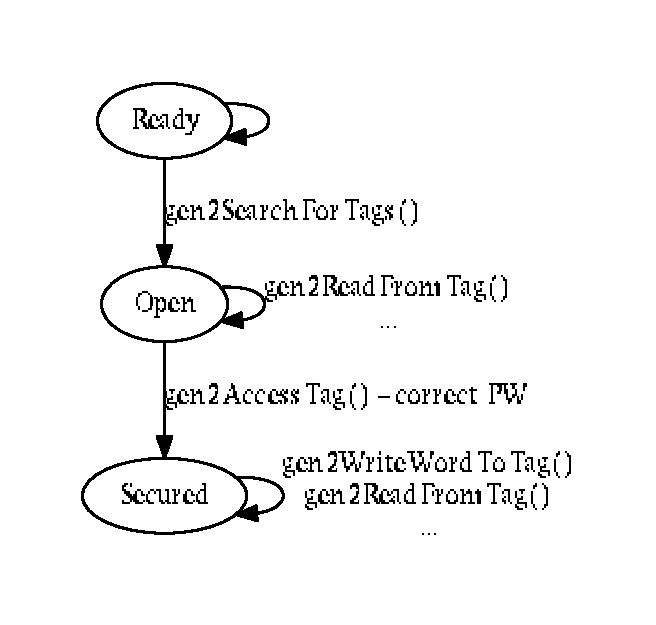
\includegraphics[width=\textwidth,height=\textheight/2,keepaspectratio=true]{dot_inline_dotgraph_1}}
\end{DoxyImageNoCaption}
\end{center}


If the tag in question does {\bfseries not} have a password set\-: \begin{center}

\begin{DoxyImageNoCaption}
  \mbox{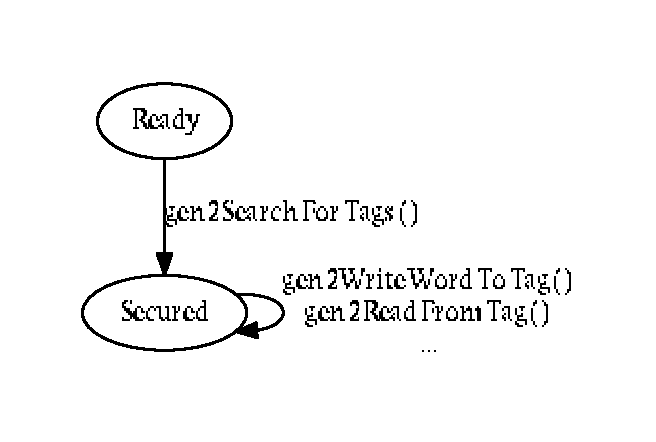
\includegraphics[width=\textwidth,height=\textheight/2,keepaspectratio=true]{dot_inline_dotgraph_2}}
\end{DoxyImageNoCaption}
\end{center}


So a typical use case may look like this\-: 
\begin{DoxyCode}
* Tag tags[16];
* \textcolor{keyword}{struct }gen2Config config = \{GEN2_LF_160, GEN2_COD_MILLER2, GEN2_IINV_S0, 1\};
* \textcolor{keywordtype}{unsigned} n;
* u8 buf[4];
* ...
* as399xInitialize(912000);
*
* gen2Open(&config);
*
* n = gen2SearchForTags(tags,16,0,0,4);
* \textcolor{keywordflow}{if} ( n == 0) \textcolor{keywordflow}{return};
*
* \textcolor{comment}{//Pick one of the tags based on the contents of tags. Here we use the very first tag}
*
* \textcolor{keywordflow}{if} (gen2ReadFromTag(tags+0, MEM_USER, 0, 2, buf))
*     \textcolor{keywordflow}{return};
*
* buf[0] ^= 0xff; buf[1]^= 0x55; \textcolor{comment}{// change the data}
*
* \textcolor{keywordflow}{if} (gen2WriteWordToTag( tags+0, MEM_USER, 0,  buf))
* \{ \textcolor{comment}{// wrote back one of the two read words}
*     gen2Close();
*     \textcolor{keywordflow}{return};
* \}
*
* \textcolor{comment}{//...}
*
* gen2Close();
*
* 
\end{DoxyCode}
 

Definition in file {\bf gen2.\-h}.



\subsection{Macro Definition Documentation}
\index{gen2.\-h@{gen2.\-h}!G\-E\-N2\-\_\-\-C\-O\-D\-\_\-\-F\-M0@{G\-E\-N2\-\_\-\-C\-O\-D\-\_\-\-F\-M0}}
\index{G\-E\-N2\-\_\-\-C\-O\-D\-\_\-\-F\-M0@{G\-E\-N2\-\_\-\-C\-O\-D\-\_\-\-F\-M0}!gen2.h@{gen2.\-h}}
\subsubsection[{G\-E\-N2\-\_\-\-C\-O\-D\-\_\-\-F\-M0}]{\setlength{\rightskip}{0pt plus 5cm}\#define G\-E\-N2\-\_\-\-C\-O\-D\-\_\-\-F\-M0~0}\label{gen2_8h_ace946adf4ab2f106e691c69c33385b05}
Rx coding values F\-M coding for rx 

Definition at line 118 of file gen2.\-h.

\index{gen2.\-h@{gen2.\-h}!G\-E\-N2\-\_\-\-C\-O\-D\-\_\-\-M\-I\-L\-L\-E\-R2@{G\-E\-N2\-\_\-\-C\-O\-D\-\_\-\-M\-I\-L\-L\-E\-R2}}
\index{G\-E\-N2\-\_\-\-C\-O\-D\-\_\-\-M\-I\-L\-L\-E\-R2@{G\-E\-N2\-\_\-\-C\-O\-D\-\_\-\-M\-I\-L\-L\-E\-R2}!gen2.h@{gen2.\-h}}
\subsubsection[{G\-E\-N2\-\_\-\-C\-O\-D\-\_\-\-M\-I\-L\-L\-E\-R2}]{\setlength{\rightskip}{0pt plus 5cm}\#define G\-E\-N2\-\_\-\-C\-O\-D\-\_\-\-M\-I\-L\-L\-E\-R2~1}\label{gen2_8h_ac85f41622cb17da8ceda2bcc31305889}
M\-I\-L\-L\-E\-R2 coding for rx 

Definition at line 119 of file gen2.\-h.

\index{gen2.\-h@{gen2.\-h}!G\-E\-N2\-\_\-\-C\-O\-D\-\_\-\-M\-I\-L\-L\-E\-R4@{G\-E\-N2\-\_\-\-C\-O\-D\-\_\-\-M\-I\-L\-L\-E\-R4}}
\index{G\-E\-N2\-\_\-\-C\-O\-D\-\_\-\-M\-I\-L\-L\-E\-R4@{G\-E\-N2\-\_\-\-C\-O\-D\-\_\-\-M\-I\-L\-L\-E\-R4}!gen2.h@{gen2.\-h}}
\subsubsection[{G\-E\-N2\-\_\-\-C\-O\-D\-\_\-\-M\-I\-L\-L\-E\-R4}]{\setlength{\rightskip}{0pt plus 5cm}\#define G\-E\-N2\-\_\-\-C\-O\-D\-\_\-\-M\-I\-L\-L\-E\-R4~2}\label{gen2_8h_a77c91fd0db1ec277b9f9b4f776d7bd90}
M\-I\-L\-L\-E\-R4 coding for rx 

Definition at line 120 of file gen2.\-h.

\index{gen2.\-h@{gen2.\-h}!G\-E\-N2\-\_\-\-C\-O\-D\-\_\-\-M\-I\-L\-L\-E\-R8@{G\-E\-N2\-\_\-\-C\-O\-D\-\_\-\-M\-I\-L\-L\-E\-R8}}
\index{G\-E\-N2\-\_\-\-C\-O\-D\-\_\-\-M\-I\-L\-L\-E\-R8@{G\-E\-N2\-\_\-\-C\-O\-D\-\_\-\-M\-I\-L\-L\-E\-R8}!gen2.h@{gen2.\-h}}
\subsubsection[{G\-E\-N2\-\_\-\-C\-O\-D\-\_\-\-M\-I\-L\-L\-E\-R8}]{\setlength{\rightskip}{0pt plus 5cm}\#define G\-E\-N2\-\_\-\-C\-O\-D\-\_\-\-M\-I\-L\-L\-E\-R8~3}\label{gen2_8h_a3d75ee65f59165c1d0dd9dd2799d2ee5}
M\-I\-L\-L\-E\-R8 coding for rx 

Definition at line 121 of file gen2.\-h.

\index{gen2.\-h@{gen2.\-h}!G\-E\-N2\-\_\-\-C\-R\-C@{G\-E\-N2\-\_\-\-C\-R\-C}}
\index{G\-E\-N2\-\_\-\-C\-R\-C@{G\-E\-N2\-\_\-\-C\-R\-C}!gen2.h@{gen2.\-h}}
\subsubsection[{G\-E\-N2\-\_\-\-C\-R\-C}]{\setlength{\rightskip}{0pt plus 5cm}\#define G\-E\-N2\-\_\-\-C\-R\-C~11}\label{gen2_8h_acae5e7db36ced48a9acd0a5fe634ac7c}
Error C\-R\-C 

Definition at line 179 of file gen2.\-h.

\index{gen2.\-h@{gen2.\-h}!G\-E\-N2\-\_\-\-E\-R\-R\-\_\-\-A\-C\-C\-E\-S\-S@{G\-E\-N2\-\_\-\-E\-R\-R\-\_\-\-A\-C\-C\-E\-S\-S}}
\index{G\-E\-N2\-\_\-\-E\-R\-R\-\_\-\-A\-C\-C\-E\-S\-S@{G\-E\-N2\-\_\-\-E\-R\-R\-\_\-\-A\-C\-C\-E\-S\-S}!gen2.h@{gen2.\-h}}
\subsubsection[{G\-E\-N2\-\_\-\-E\-R\-R\-\_\-\-A\-C\-C\-E\-S\-S}]{\setlength{\rightskip}{0pt plus 5cm}\#define G\-E\-N2\-\_\-\-E\-R\-R\-\_\-\-A\-C\-C\-E\-S\-S~2}\label{gen2_8h_ad10be1495a3215566ac5d25b31bc99fa}
Error sending Access password 

Definition at line 170 of file gen2.\-h.

\index{gen2.\-h@{gen2.\-h}!G\-E\-N2\-\_\-\-E\-R\-R\-\_\-\-B\-L\-O\-C\-K\-E\-R\-A\-S\-E@{G\-E\-N2\-\_\-\-E\-R\-R\-\_\-\-B\-L\-O\-C\-K\-E\-R\-A\-S\-E}}
\index{G\-E\-N2\-\_\-\-E\-R\-R\-\_\-\-B\-L\-O\-C\-K\-E\-R\-A\-S\-E@{G\-E\-N2\-\_\-\-E\-R\-R\-\_\-\-B\-L\-O\-C\-K\-E\-R\-A\-S\-E}!gen2.h@{gen2.\-h}}
\subsubsection[{G\-E\-N2\-\_\-\-E\-R\-R\-\_\-\-B\-L\-O\-C\-K\-E\-R\-A\-S\-E}]{\setlength{\rightskip}{0pt plus 5cm}\#define G\-E\-N2\-\_\-\-E\-R\-R\-\_\-\-B\-L\-O\-C\-K\-E\-R\-A\-S\-E~7}\label{gen2_8h_ae6671e57548044547444f407d4690415}
Erorr Blockerase 

Definition at line 175 of file gen2.\-h.

\index{gen2.\-h@{gen2.\-h}!G\-E\-N2\-\_\-\-E\-R\-R\-\_\-\-B\-L\-O\-C\-K\-W\-R\-I\-T\-E@{G\-E\-N2\-\_\-\-E\-R\-R\-\_\-\-B\-L\-O\-C\-K\-W\-R\-I\-T\-E}}
\index{G\-E\-N2\-\_\-\-E\-R\-R\-\_\-\-B\-L\-O\-C\-K\-W\-R\-I\-T\-E@{G\-E\-N2\-\_\-\-E\-R\-R\-\_\-\-B\-L\-O\-C\-K\-W\-R\-I\-T\-E}!gen2.h@{gen2.\-h}}
\subsubsection[{G\-E\-N2\-\_\-\-E\-R\-R\-\_\-\-B\-L\-O\-C\-K\-W\-R\-I\-T\-E}]{\setlength{\rightskip}{0pt plus 5cm}\#define G\-E\-N2\-\_\-\-E\-R\-R\-\_\-\-B\-L\-O\-C\-K\-W\-R\-I\-T\-E~6}\label{gen2_8h_a6ba426677897eae0421b6f7585265de8}
Error Blockwrite 

Definition at line 174 of file gen2.\-h.

\index{gen2.\-h@{gen2.\-h}!G\-E\-N2\-\_\-\-E\-R\-R\-\_\-\-C\-H\-A\-N\-N\-E\-L\-\_\-\-T\-I\-M\-E\-O\-U\-T@{G\-E\-N2\-\_\-\-E\-R\-R\-\_\-\-C\-H\-A\-N\-N\-E\-L\-\_\-\-T\-I\-M\-E\-O\-U\-T}}
\index{G\-E\-N2\-\_\-\-E\-R\-R\-\_\-\-C\-H\-A\-N\-N\-E\-L\-\_\-\-T\-I\-M\-E\-O\-U\-T@{G\-E\-N2\-\_\-\-E\-R\-R\-\_\-\-C\-H\-A\-N\-N\-E\-L\-\_\-\-T\-I\-M\-E\-O\-U\-T}!gen2.h@{gen2.\-h}}
\subsubsection[{G\-E\-N2\-\_\-\-E\-R\-R\-\_\-\-C\-H\-A\-N\-N\-E\-L\-\_\-\-T\-I\-M\-E\-O\-U\-T}]{\setlength{\rightskip}{0pt plus 5cm}\#define G\-E\-N2\-\_\-\-E\-R\-R\-\_\-\-C\-H\-A\-N\-N\-E\-L\-\_\-\-T\-I\-M\-E\-O\-U\-T~10}\label{gen2_8h_a40d64d46e53f311dc60f014b4f8956c3}
Error R\-F channel timed out 

Definition at line 178 of file gen2.\-h.

\index{gen2.\-h@{gen2.\-h}!G\-E\-N2\-\_\-\-E\-R\-R\-\_\-\-K\-I\-L\-L@{G\-E\-N2\-\_\-\-E\-R\-R\-\_\-\-K\-I\-L\-L}}
\index{G\-E\-N2\-\_\-\-E\-R\-R\-\_\-\-K\-I\-L\-L@{G\-E\-N2\-\_\-\-E\-R\-R\-\_\-\-K\-I\-L\-L}!gen2.h@{gen2.\-h}}
\subsubsection[{G\-E\-N2\-\_\-\-E\-R\-R\-\_\-\-K\-I\-L\-L}]{\setlength{\rightskip}{0pt plus 5cm}\#define G\-E\-N2\-\_\-\-E\-R\-R\-\_\-\-K\-I\-L\-L~3}\label{gen2_8h_a8f124c1e2f6cc893874faed81eb1cd7e}
Error sending Kill 

Definition at line 171 of file gen2.\-h.

\index{gen2.\-h@{gen2.\-h}!G\-E\-N2\-\_\-\-E\-R\-R\-\_\-\-L\-O\-C\-K@{G\-E\-N2\-\_\-\-E\-R\-R\-\_\-\-L\-O\-C\-K}}
\index{G\-E\-N2\-\_\-\-E\-R\-R\-\_\-\-L\-O\-C\-K@{G\-E\-N2\-\_\-\-E\-R\-R\-\_\-\-L\-O\-C\-K}!gen2.h@{gen2.\-h}}
\subsubsection[{G\-E\-N2\-\_\-\-E\-R\-R\-\_\-\-L\-O\-C\-K}]{\setlength{\rightskip}{0pt plus 5cm}\#define G\-E\-N2\-\_\-\-E\-R\-R\-\_\-\-L\-O\-C\-K~5}\label{gen2_8h_a37f840b78e38f06ab02d5c2922b19404}
Error locking command 

Definition at line 173 of file gen2.\-h.

\index{gen2.\-h@{gen2.\-h}!G\-E\-N2\-\_\-\-E\-R\-R\-\_\-\-N\-O\-R\-E\-P\-L\-Y@{G\-E\-N2\-\_\-\-E\-R\-R\-\_\-\-N\-O\-R\-E\-P\-L\-Y}}
\index{G\-E\-N2\-\_\-\-E\-R\-R\-\_\-\-N\-O\-R\-E\-P\-L\-Y@{G\-E\-N2\-\_\-\-E\-R\-R\-\_\-\-N\-O\-R\-E\-P\-L\-Y}!gen2.h@{gen2.\-h}}
\subsubsection[{G\-E\-N2\-\_\-\-E\-R\-R\-\_\-\-N\-O\-R\-E\-P\-L\-Y}]{\setlength{\rightskip}{0pt plus 5cm}\#define G\-E\-N2\-\_\-\-E\-R\-R\-\_\-\-N\-O\-R\-E\-P\-L\-Y~4}\label{gen2_8h_a4127dbe4357f2c783638d22718b4430a}
Error no reply received 

Definition at line 172 of file gen2.\-h.

\index{gen2.\-h@{gen2.\-h}!G\-E\-N2\-\_\-\-E\-R\-R\-\_\-\-R\-E\-A\-D@{G\-E\-N2\-\_\-\-E\-R\-R\-\_\-\-R\-E\-A\-D}}
\index{G\-E\-N2\-\_\-\-E\-R\-R\-\_\-\-R\-E\-A\-D@{G\-E\-N2\-\_\-\-E\-R\-R\-\_\-\-R\-E\-A\-D}!gen2.h@{gen2.\-h}}
\subsubsection[{G\-E\-N2\-\_\-\-E\-R\-R\-\_\-\-R\-E\-A\-D}]{\setlength{\rightskip}{0pt plus 5cm}\#define G\-E\-N2\-\_\-\-E\-R\-R\-\_\-\-R\-E\-A\-D~8}\label{gen2_8h_a7669ecdfdf2ba1206c1c7436a2e44821}
Error Reading 

Definition at line 176 of file gen2.\-h.

\index{gen2.\-h@{gen2.\-h}!G\-E\-N2\-\_\-\-E\-R\-R\-\_\-\-R\-E\-Q\-R\-N@{G\-E\-N2\-\_\-\-E\-R\-R\-\_\-\-R\-E\-Q\-R\-N}}
\index{G\-E\-N2\-\_\-\-E\-R\-R\-\_\-\-R\-E\-Q\-R\-N@{G\-E\-N2\-\_\-\-E\-R\-R\-\_\-\-R\-E\-Q\-R\-N}!gen2.h@{gen2.\-h}}
\subsubsection[{G\-E\-N2\-\_\-\-E\-R\-R\-\_\-\-R\-E\-Q\-R\-N}]{\setlength{\rightskip}{0pt plus 5cm}\#define G\-E\-N2\-\_\-\-E\-R\-R\-\_\-\-R\-E\-Q\-R\-N~1}\label{gen2_8h_a95bfaf45650135b2c8a38e173167169d}
Error sending Req\-R\-N 

Definition at line 169 of file gen2.\-h.

\index{gen2.\-h@{gen2.\-h}!G\-E\-N2\-\_\-\-E\-R\-R\-\_\-\-S\-E\-L\-E\-C\-T@{G\-E\-N2\-\_\-\-E\-R\-R\-\_\-\-S\-E\-L\-E\-C\-T}}
\index{G\-E\-N2\-\_\-\-E\-R\-R\-\_\-\-S\-E\-L\-E\-C\-T@{G\-E\-N2\-\_\-\-E\-R\-R\-\_\-\-S\-E\-L\-E\-C\-T}!gen2.h@{gen2.\-h}}
\subsubsection[{G\-E\-N2\-\_\-\-E\-R\-R\-\_\-\-S\-E\-L\-E\-C\-T}]{\setlength{\rightskip}{0pt plus 5cm}\#define G\-E\-N2\-\_\-\-E\-R\-R\-\_\-\-S\-E\-L\-E\-C\-T~9}\label{gen2_8h_a96cf4fc05783673da0607b14230bb215}
Error when selecting tag 

Definition at line 177 of file gen2.\-h.

\index{gen2.\-h@{gen2.\-h}!G\-E\-N2\-\_\-\-I\-I\-N\-V\-\_\-\-S0@{G\-E\-N2\-\_\-\-I\-I\-N\-V\-\_\-\-S0}}
\index{G\-E\-N2\-\_\-\-I\-I\-N\-V\-\_\-\-S0@{G\-E\-N2\-\_\-\-I\-I\-N\-V\-\_\-\-S0}!gen2.h@{gen2.\-h}}
\subsubsection[{G\-E\-N2\-\_\-\-I\-I\-N\-V\-\_\-\-S0}]{\setlength{\rightskip}{0pt plus 5cm}\#define G\-E\-N2\-\_\-\-I\-I\-N\-V\-\_\-\-S0~0x00 /$\ast$\-Inventoried (\-S0) $\ast$/}\label{gen2_8h_ac3cad8cdfeb77e51e563a6ef2e064f86}
Definition for inventory\-: Inventoried (S0) 

Definition at line 151 of file gen2.\-h.

\index{gen2.\-h@{gen2.\-h}!G\-E\-N2\-\_\-\-I\-I\-N\-V\-\_\-\-S1@{G\-E\-N2\-\_\-\-I\-I\-N\-V\-\_\-\-S1}}
\index{G\-E\-N2\-\_\-\-I\-I\-N\-V\-\_\-\-S1@{G\-E\-N2\-\_\-\-I\-I\-N\-V\-\_\-\-S1}!gen2.h@{gen2.\-h}}
\subsubsection[{G\-E\-N2\-\_\-\-I\-I\-N\-V\-\_\-\-S1}]{\setlength{\rightskip}{0pt plus 5cm}\#define G\-E\-N2\-\_\-\-I\-I\-N\-V\-\_\-\-S1~0x01 /$\ast$001\-: Inventoried (\-S1) $\ast$/}\label{gen2_8h_aa32184057f6decdb37faa8b90f785358}
Definition for inventory\-: 001\-: Inventoried (S1) 

Definition at line 153 of file gen2.\-h.

\index{gen2.\-h@{gen2.\-h}!G\-E\-N2\-\_\-\-I\-I\-N\-V\-\_\-\-S2@{G\-E\-N2\-\_\-\-I\-I\-N\-V\-\_\-\-S2}}
\index{G\-E\-N2\-\_\-\-I\-I\-N\-V\-\_\-\-S2@{G\-E\-N2\-\_\-\-I\-I\-N\-V\-\_\-\-S2}!gen2.h@{gen2.\-h}}
\subsubsection[{G\-E\-N2\-\_\-\-I\-I\-N\-V\-\_\-\-S2}]{\setlength{\rightskip}{0pt plus 5cm}\#define G\-E\-N2\-\_\-\-I\-I\-N\-V\-\_\-\-S2~0x02 /$\ast$010\-: Inventoried (\-S2) $\ast$/}\label{gen2_8h_afa73ea6c3aa8ac80bdbc68e2a598f598}
Definition for inventory\-: 010\-: Inventoried (S2) 

Definition at line 155 of file gen2.\-h.

\index{gen2.\-h@{gen2.\-h}!G\-E\-N2\-\_\-\-I\-I\-N\-V\-\_\-\-S3@{G\-E\-N2\-\_\-\-I\-I\-N\-V\-\_\-\-S3}}
\index{G\-E\-N2\-\_\-\-I\-I\-N\-V\-\_\-\-S3@{G\-E\-N2\-\_\-\-I\-I\-N\-V\-\_\-\-S3}!gen2.h@{gen2.\-h}}
\subsubsection[{G\-E\-N2\-\_\-\-I\-I\-N\-V\-\_\-\-S3}]{\setlength{\rightskip}{0pt plus 5cm}\#define G\-E\-N2\-\_\-\-I\-I\-N\-V\-\_\-\-S3~0x03 /$\ast$011\-: Inventoried (\-S3) $\ast$/}\label{gen2_8h_add3e5dbcc9f23b021792c28a35e741c2}
Definition for inventory\-: 011\-: Inventoried (S3) 

Definition at line 157 of file gen2.\-h.

\index{gen2.\-h@{gen2.\-h}!G\-E\-N2\-\_\-\-I\-I\-N\-V\-\_\-\-S\-L@{G\-E\-N2\-\_\-\-I\-I\-N\-V\-\_\-\-S\-L}}
\index{G\-E\-N2\-\_\-\-I\-I\-N\-V\-\_\-\-S\-L@{G\-E\-N2\-\_\-\-I\-I\-N\-V\-\_\-\-S\-L}!gen2.h@{gen2.\-h}}
\subsubsection[{G\-E\-N2\-\_\-\-I\-I\-N\-V\-\_\-\-S\-L}]{\setlength{\rightskip}{0pt plus 5cm}\#define G\-E\-N2\-\_\-\-I\-I\-N\-V\-\_\-\-S\-L~0x04 /$\ast$100\-: S\-L $\ast$/}\label{gen2_8h_a662d6a01220e2354752cb965915f6b22}
Definition for inventory\-: 100\-: S\-L 

Definition at line 159 of file gen2.\-h.

\index{gen2.\-h@{gen2.\-h}!G\-E\-N2\-\_\-\-L\-F\-\_\-160@{G\-E\-N2\-\_\-\-L\-F\-\_\-160}}
\index{G\-E\-N2\-\_\-\-L\-F\-\_\-160@{G\-E\-N2\-\_\-\-L\-F\-\_\-160}!gen2.h@{gen2.\-h}}
\subsubsection[{G\-E\-N2\-\_\-\-L\-F\-\_\-160}]{\setlength{\rightskip}{0pt plus 5cm}\#define G\-E\-N2\-\_\-\-L\-F\-\_\-160~6}\label{gen2_8h_abcaca3a157e02fcd7525a12254a83cc6}
link frequency 160 k\-Hz 

Definition at line 111 of file gen2.\-h.

\index{gen2.\-h@{gen2.\-h}!G\-E\-N2\-\_\-\-L\-F\-\_\-213@{G\-E\-N2\-\_\-\-L\-F\-\_\-213}}
\index{G\-E\-N2\-\_\-\-L\-F\-\_\-213@{G\-E\-N2\-\_\-\-L\-F\-\_\-213}!gen2.h@{gen2.\-h}}
\subsubsection[{G\-E\-N2\-\_\-\-L\-F\-\_\-213}]{\setlength{\rightskip}{0pt plus 5cm}\#define G\-E\-N2\-\_\-\-L\-F\-\_\-213~8}\label{gen2_8h_a2aca1df657bed3cf383942b93edd6481}
link frequency 213 k\-Hz 

Definition at line 112 of file gen2.\-h.

\index{gen2.\-h@{gen2.\-h}!G\-E\-N2\-\_\-\-L\-F\-\_\-256@{G\-E\-N2\-\_\-\-L\-F\-\_\-256}}
\index{G\-E\-N2\-\_\-\-L\-F\-\_\-256@{G\-E\-N2\-\_\-\-L\-F\-\_\-256}!gen2.h@{gen2.\-h}}
\subsubsection[{G\-E\-N2\-\_\-\-L\-F\-\_\-256}]{\setlength{\rightskip}{0pt plus 5cm}\#define G\-E\-N2\-\_\-\-L\-F\-\_\-256~9}\label{gen2_8h_af35ffd318208fc1c0173928622b8df03}
link frequency 213 k\-Hz 

Definition at line 113 of file gen2.\-h.

\index{gen2.\-h@{gen2.\-h}!G\-E\-N2\-\_\-\-L\-F\-\_\-320@{G\-E\-N2\-\_\-\-L\-F\-\_\-320}}
\index{G\-E\-N2\-\_\-\-L\-F\-\_\-320@{G\-E\-N2\-\_\-\-L\-F\-\_\-320}!gen2.h@{gen2.\-h}}
\subsubsection[{G\-E\-N2\-\_\-\-L\-F\-\_\-320}]{\setlength{\rightskip}{0pt plus 5cm}\#define G\-E\-N2\-\_\-\-L\-F\-\_\-320~12}\label{gen2_8h_ab93f1d4b1117691572e84bb7c4ed5d09}
link frequency 213 k\-Hz 

Definition at line 114 of file gen2.\-h.

\index{gen2.\-h@{gen2.\-h}!G\-E\-N2\-\_\-\-L\-F\-\_\-40@{G\-E\-N2\-\_\-\-L\-F\-\_\-40}}
\index{G\-E\-N2\-\_\-\-L\-F\-\_\-40@{G\-E\-N2\-\_\-\-L\-F\-\_\-40}!gen2.h@{gen2.\-h}}
\subsubsection[{G\-E\-N2\-\_\-\-L\-F\-\_\-40}]{\setlength{\rightskip}{0pt plus 5cm}\#define G\-E\-N2\-\_\-\-L\-F\-\_\-40~0}\label{gen2_8h_a3e6814a35194e7d169c2a31b0ef1a79c}
link frequency 40 k\-Hz 

Definition at line 107 of file gen2.\-h.

\index{gen2.\-h@{gen2.\-h}!G\-E\-N2\-\_\-\-L\-F\-\_\-640@{G\-E\-N2\-\_\-\-L\-F\-\_\-640}}
\index{G\-E\-N2\-\_\-\-L\-F\-\_\-640@{G\-E\-N2\-\_\-\-L\-F\-\_\-640}!gen2.h@{gen2.\-h}}
\subsubsection[{G\-E\-N2\-\_\-\-L\-F\-\_\-640}]{\setlength{\rightskip}{0pt plus 5cm}\#define G\-E\-N2\-\_\-\-L\-F\-\_\-640~15}\label{gen2_8h_adb272c7cfabadaee950371b9c8d0d7b0}
link frequency 640 k\-Hz 

Definition at line 115 of file gen2.\-h.

\index{gen2.\-h@{gen2.\-h}!G\-E\-N2\-\_\-\-O\-K@{G\-E\-N2\-\_\-\-O\-K}}
\index{G\-E\-N2\-\_\-\-O\-K@{G\-E\-N2\-\_\-\-O\-K}!gen2.h@{gen2.\-h}}
\subsubsection[{G\-E\-N2\-\_\-\-O\-K}]{\setlength{\rightskip}{0pt plus 5cm}\#define G\-E\-N2\-\_\-\-O\-K~0}\label{gen2_8h_a4724a40ebda0e970e52d4cca2b4491f5}
Defines for various return codes No error 

Definition at line 168 of file gen2.\-h.

\index{gen2.\-h@{gen2.\-h}!M\-E\-M\-\_\-\-E\-P\-C@{M\-E\-M\-\_\-\-E\-P\-C}}
\index{M\-E\-M\-\_\-\-E\-P\-C@{M\-E\-M\-\_\-\-E\-P\-C}!gen2.h@{gen2.\-h}}
\subsubsection[{M\-E\-M\-\_\-\-E\-P\-C}]{\setlength{\rightskip}{0pt plus 5cm}\#define M\-E\-M\-\_\-\-E\-P\-C~0x01}\label{gen2_8h_aa56d3b9ae1f5a4f7893e7e4c24abc95b}
Definition for E\-P\-C tag memory bank\-: E\-P\-C memory 

Definition at line 127 of file gen2.\-h.

\index{gen2.\-h@{gen2.\-h}!M\-E\-M\-\_\-\-R\-E\-S@{M\-E\-M\-\_\-\-R\-E\-S}}
\index{M\-E\-M\-\_\-\-R\-E\-S@{M\-E\-M\-\_\-\-R\-E\-S}!gen2.h@{gen2.\-h}}
\subsubsection[{M\-E\-M\-\_\-\-R\-E\-S}]{\setlength{\rightskip}{0pt plus 5cm}\#define M\-E\-M\-\_\-\-R\-E\-S~0x00}\label{gen2_8h_a88a66b76a94385774cfdeae423ef0792}
Definition for E\-P\-C tag memory bank\-: reserved 

Definition at line 125 of file gen2.\-h.

\index{gen2.\-h@{gen2.\-h}!M\-E\-M\-\_\-\-T\-I\-D@{M\-E\-M\-\_\-\-T\-I\-D}}
\index{M\-E\-M\-\_\-\-T\-I\-D@{M\-E\-M\-\_\-\-T\-I\-D}!gen2.h@{gen2.\-h}}
\subsubsection[{M\-E\-M\-\_\-\-T\-I\-D}]{\setlength{\rightskip}{0pt plus 5cm}\#define M\-E\-M\-\_\-\-T\-I\-D~0x02}\label{gen2_8h_a274f23ac2bc4875711bab00f28704a89}
Definition for E\-P\-C tag memory bank\-: T\-I\-D 

Definition at line 129 of file gen2.\-h.

\index{gen2.\-h@{gen2.\-h}!M\-E\-M\-\_\-\-U\-S\-E\-R@{M\-E\-M\-\_\-\-U\-S\-E\-R}}
\index{M\-E\-M\-\_\-\-U\-S\-E\-R@{M\-E\-M\-\_\-\-U\-S\-E\-R}!gen2.h@{gen2.\-h}}
\subsubsection[{M\-E\-M\-\_\-\-U\-S\-E\-R}]{\setlength{\rightskip}{0pt plus 5cm}\#define M\-E\-M\-\_\-\-U\-S\-E\-R~0x03}\label{gen2_8h_a1168f49bb6b4954943fba4baa4a6ea8f}
Definition for E\-P\-C tag memory bank\-: user 

Definition at line 131 of file gen2.\-h.

\index{gen2.\-h@{gen2.\-h}!M\-E\-M\-A\-D\-R\-\_\-\-A\-C\-C\-E\-S\-S\-P\-W\-D@{M\-E\-M\-A\-D\-R\-\_\-\-A\-C\-C\-E\-S\-S\-P\-W\-D}}
\index{M\-E\-M\-A\-D\-R\-\_\-\-A\-C\-C\-E\-S\-S\-P\-W\-D@{M\-E\-M\-A\-D\-R\-\_\-\-A\-C\-C\-E\-S\-S\-P\-W\-D}!gen2.h@{gen2.\-h}}
\subsubsection[{M\-E\-M\-A\-D\-R\-\_\-\-A\-C\-C\-E\-S\-S\-P\-W\-D}]{\setlength{\rightskip}{0pt plus 5cm}\#define M\-E\-M\-A\-D\-R\-\_\-\-A\-C\-C\-E\-S\-S\-P\-W\-D~0x02}\label{gen2_8h_a1a9187c94d0915d913e72718cba08ef0}
Definition for E\-P\-C wordpointer\-: Address for access password value 

Definition at line 144 of file gen2.\-h.

\index{gen2.\-h@{gen2.\-h}!M\-E\-M\-A\-D\-R\-\_\-\-C\-R\-C@{M\-E\-M\-A\-D\-R\-\_\-\-C\-R\-C}}
\index{M\-E\-M\-A\-D\-R\-\_\-\-C\-R\-C@{M\-E\-M\-A\-D\-R\-\_\-\-C\-R\-C}!gen2.h@{gen2.\-h}}
\subsubsection[{M\-E\-M\-A\-D\-R\-\_\-\-C\-R\-C}]{\setlength{\rightskip}{0pt plus 5cm}\#define M\-E\-M\-A\-D\-R\-\_\-\-C\-R\-C~0x00}\label{gen2_8h_aa12d4093b4053058a80d0278f2ce485f}
Definition for E\-P\-C wordpointer\-: Address for C\-R\-C value 

Definition at line 135 of file gen2.\-h.

\index{gen2.\-h@{gen2.\-h}!M\-E\-M\-A\-D\-R\-\_\-\-E\-P\-C@{M\-E\-M\-A\-D\-R\-\_\-\-E\-P\-C}}
\index{M\-E\-M\-A\-D\-R\-\_\-\-E\-P\-C@{M\-E\-M\-A\-D\-R\-\_\-\-E\-P\-C}!gen2.h@{gen2.\-h}}
\subsubsection[{M\-E\-M\-A\-D\-R\-\_\-\-E\-P\-C}]{\setlength{\rightskip}{0pt plus 5cm}\#define M\-E\-M\-A\-D\-R\-\_\-\-E\-P\-C~0x02}\label{gen2_8h_afbb658518070433a3a00f15e7c6342bc}
Definition for E\-P\-C wordpointer\-: Address for E\-P\-C value 

Definition at line 139 of file gen2.\-h.

\index{gen2.\-h@{gen2.\-h}!M\-E\-M\-A\-D\-R\-\_\-\-K\-I\-L\-L\-P\-W\-D@{M\-E\-M\-A\-D\-R\-\_\-\-K\-I\-L\-L\-P\-W\-D}}
\index{M\-E\-M\-A\-D\-R\-\_\-\-K\-I\-L\-L\-P\-W\-D@{M\-E\-M\-A\-D\-R\-\_\-\-K\-I\-L\-L\-P\-W\-D}!gen2.h@{gen2.\-h}}
\subsubsection[{M\-E\-M\-A\-D\-R\-\_\-\-K\-I\-L\-L\-P\-W\-D}]{\setlength{\rightskip}{0pt plus 5cm}\#define M\-E\-M\-A\-D\-R\-\_\-\-K\-I\-L\-L\-P\-W\-D~0x00}\label{gen2_8h_a16160f52091439d8b864d5cac82086b0}
Definition for E\-P\-C wordpointer\-: Address for kill password value 

Definition at line 142 of file gen2.\-h.

\index{gen2.\-h@{gen2.\-h}!M\-E\-M\-A\-D\-R\-\_\-\-P\-C@{M\-E\-M\-A\-D\-R\-\_\-\-P\-C}}
\index{M\-E\-M\-A\-D\-R\-\_\-\-P\-C@{M\-E\-M\-A\-D\-R\-\_\-\-P\-C}!gen2.h@{gen2.\-h}}
\subsubsection[{M\-E\-M\-A\-D\-R\-\_\-\-P\-C}]{\setlength{\rightskip}{0pt plus 5cm}\#define M\-E\-M\-A\-D\-R\-\_\-\-P\-C~0x01}\label{gen2_8h_aa832082f9f3309256f4e3f235c9b6b6c}
Definition for E\-P\-C wordpointer\-: Address for P\-C value Word position 

Definition at line 137 of file gen2.\-h.

\index{gen2.\-h@{gen2.\-h}!M\-E\-M\-A\-D\-R\-\_\-\-T\-I\-D@{M\-E\-M\-A\-D\-R\-\_\-\-T\-I\-D}}
\index{M\-E\-M\-A\-D\-R\-\_\-\-T\-I\-D@{M\-E\-M\-A\-D\-R\-\_\-\-T\-I\-D}!gen2.h@{gen2.\-h}}
\subsubsection[{M\-E\-M\-A\-D\-R\-\_\-\-T\-I\-D}]{\setlength{\rightskip}{0pt plus 5cm}\#define M\-E\-M\-A\-D\-R\-\_\-\-T\-I\-D~0x00}\label{gen2_8h_a7731be4651f241fa77a07e95b503b800}
Definition for E\-P\-C wordpointer\-: Address for T\-I\-D value 

Definition at line 147 of file gen2.\-h.



\subsection{Function Documentation}
\index{gen2.\-h@{gen2.\-h}!gen2\-Access\-Tag@{gen2\-Access\-Tag}}
\index{gen2\-Access\-Tag@{gen2\-Access\-Tag}!gen2.h@{gen2.\-h}}
\subsubsection[{gen2\-Access\-Tag}]{\setlength{\rightskip}{0pt plus 5cm}{\bf u8} gen2\-Access\-Tag (
\begin{DoxyParamCaption}
\item[{{\bf Tag} $\ast$}]{tag, }
\item[{{\bf u8} $\ast$}]{password}
\end{DoxyParamCaption}
)}\label{gen2_8h_a3adf4cc7b53a5bcec846776bd7ef7c4e}
E\-P\-C A\-C\-C\-E\-S\-S command send to the Tag. This function is used to bring a tag with set access password from the Open state to the Secured state.

\begin{DoxyAttention}{Attention}
This command works on the one tag which is currently in the open state, i.\-e. on the last tag found by \doxyref{gen2\-Search\-For\-Tags()}{p.}{gen2_8c_acc4bef39e563061789915a8fefadb080}.
\end{DoxyAttention}

\begin{DoxyParams}{Parameters}
{\em $\ast$tag} & Pointer to the Tag structure. \\
\hline
{\em $\ast$password} & Pointer to first byte of the access password \\
\hline
\end{DoxyParams}
\begin{DoxyReturn}{Returns}
The function returns an errorcode. 0x00 means no Error occoured. Any other value is the backscattered error code from the tag. 
\end{DoxyReturn}


Definition at line 307 of file gen2.\-c.

\index{gen2.\-h@{gen2.\-h}!gen2\-Calibrate@{gen2\-Calibrate}}
\index{gen2\-Calibrate@{gen2\-Calibrate}!gen2.h@{gen2.\-h}}
\subsubsection[{gen2\-Calibrate}]{\setlength{\rightskip}{0pt plus 5cm}{\bf u8} gen2\-Calibrate (
\begin{DoxyParamCaption}
\item[{{\bf Tag} $\ast$}]{tag}
\end{DoxyParamCaption}
)}\label{gen2_8h_a0ea6ea9eee84368ca1da42918f1fa6c4}
This function execute sthe N\-X\-P special command Calibrate

\begin{DoxyAttention}{Attention}
This command works on the one tag which is currently in the open state, i.\-e. on the last tag found by \doxyref{gen2\-Search\-For\-Tags()}{p.}{gen2_8c_acc4bef39e563061789915a8fefadb080}.
\end{DoxyAttention}

\begin{DoxyParams}{Parameters}
{\em $\ast$tag} & Pointer to the Tag structure. \\
\hline
\end{DoxyParams}


Definition at line 1591 of file gen2.\-c.

\index{gen2.\-h@{gen2.\-h}!gen2\-Challenge\-Command@{gen2\-Challenge\-Command}}
\index{gen2\-Challenge\-Command@{gen2\-Challenge\-Command}!gen2.h@{gen2.\-h}}
\subsubsection[{gen2\-Challenge\-Command}]{\setlength{\rightskip}{0pt plus 5cm}{\bf u8} gen2\-Challenge\-Command (
\begin{DoxyParamCaption}
\item[{{\bf u8}}]{command\-Flags, }
\item[{crypto\-Suite\-Id}]{, }
\item[{u16}]{msg\-Bit\-Length, }
\item[{{\bf u8} $\ast$}]{message, }
\item[{{\bf u8} $\ast$}]{output, }
\item[{{\bf u8} $\ast$}]{output\-Length}
\end{DoxyParamCaption}
)}\label{gen2_8h_a6187adc2b1b01276a94b2b1c3314cf59}
This function sends the Challenge Command D4h to all tags in range. The challenge is used to trigger all tags within range to pre-\/calculate the the crypto-\/authentication for later request when tags are selected.


\begin{DoxyParams}{Parameters}
{\em command\-Flags} & bit-\/coded command info (R\-F\-U, Buffer, Inc\-Rep\-Len, immed). \\
\hline
{\em crypto\-Suite\-Id} & Crypto Suite I\-D to define the used crypto algorithm. \\
\hline
{\em msg\-Bit\-Length} & bit length of the message (can be E\-B\-V-\/encoded for proprietary implementations). \\
\hline
{\em $\ast$message} & pointer to message bit stream. \\
\hline
{\em $\ast$output} & pointer to response buffer. \\
\hline
{\em $\ast$output\-Length} & pointer to variable which stores size of valid data in response buffer in bytes. \\
\hline
\end{DoxyParams}


Definition at line 1620 of file gen2.\-c.

\index{gen2.\-h@{gen2.\-h}!gen2\-Change\-E\-A\-S@{gen2\-Change\-E\-A\-S}}
\index{gen2\-Change\-E\-A\-S@{gen2\-Change\-E\-A\-S}!gen2.h@{gen2.\-h}}
\subsubsection[{gen2\-Change\-E\-A\-S}]{\setlength{\rightskip}{0pt plus 5cm}{\bf u8} gen2\-Change\-E\-A\-S (
\begin{DoxyParamCaption}
\item[{{\bf Tag} $\ast$}]{tag, }
\item[{{\bf u8}}]{value}
\end{DoxyParamCaption}
)}\label{gen2_8h_ad2be1d431e4b15649c99d63c628f31bf}
This function executes the N\-X\-P special command Change E\-A\-S

\begin{DoxyAttention}{Attention}
This command works on the one tag which is currently in the open state, i.\-e. on the last tag found by \doxyref{gen2\-Search\-For\-Tags()}{p.}{gen2_8c_acc4bef39e563061789915a8fefadb080}.
\end{DoxyAttention}

\begin{DoxyParams}{Parameters}
{\em $\ast$tag} & Pointer to the Tag structure. \\
\hline
{\em value} & to be set \\
\hline
\end{DoxyParams}


Definition at line 1564 of file gen2.\-c.

\index{gen2.\-h@{gen2.\-h}!gen2\-Close@{gen2\-Close}}
\index{gen2\-Close@{gen2\-Close}!gen2.h@{gen2.\-h}}
\subsubsection[{gen2\-Close}]{\setlength{\rightskip}{0pt plus 5cm}void gen2\-Close (
\begin{DoxyParamCaption}
\item[{void}]{}
\end{DoxyParamCaption}
)}\label{gen2_8h_a3ec10b438f289670b3bcd466df074740}


Close a session. 

Close the session for gen2 protocol 

Definition at line 1968 of file gen2.\-c.

\index{gen2.\-h@{gen2.\-h}!gen2\-Configure@{gen2\-Configure}}
\index{gen2\-Configure@{gen2\-Configure}!gen2.h@{gen2.\-h}}
\subsubsection[{gen2\-Configure}]{\setlength{\rightskip}{0pt plus 5cm}void gen2\-Configure (
\begin{DoxyParamCaption}
\item[{const struct gen2\-Config $\ast$}]{config}
\end{DoxyParamCaption}
)}\label{gen2_8h_ac58e25f69482315c515acce7a682c1c0}


Set the link frequency. 

Set the link frequency and gen2 specific parameters. After calling this function the A\-S3991 is in normal. 

Definition at line 1797 of file gen2.\-c.

\index{gen2.\-h@{gen2.\-h}!gen2\-Generic\-Command@{gen2\-Generic\-Command}}
\index{gen2\-Generic\-Command@{gen2\-Generic\-Command}!gen2.h@{gen2.\-h}}
\subsubsection[{gen2\-Generic\-Command}]{\setlength{\rightskip}{0pt plus 5cm}{\bf u8} gen2\-Generic\-Command (
\begin{DoxyParamCaption}
\item[{{\bf Tag} $\ast$}]{tag, }
\item[{struct gen2\-Generic\-Cmd\-Data $\ast$}]{command\-Data}
\end{DoxyParamCaption}
)}\label{gen2_8h_a35af734c0d114c8ef2c99a4f2ace0d85}
G\-E\-N\-E\-R\-I\-C C\-O\-M\-M\-A\-N\-D send to the Tag.

\begin{DoxyAttention}{Attention}
This command works on the one tag which is currently in the open state, i.\-e. on the last tag found by \doxyref{gen2\-Search\-For\-Tags()}{p.}{gen2_8c_acc4bef39e563061789915a8fefadb080}.
\end{DoxyAttention}

\begin{DoxyParams}{Parameters}
{\em $\ast$tag} & Pointer to the Tag structure. \\
\hline
{\em $\ast$command\-Data} & structure which contains all relevant data for generic command. \\
\hline
\end{DoxyParams}
\begin{DoxyReturn}{Returns}
The function returns an error-\/code. 0x00 means no error occurred. 0x\-F\-F unknown error occurred. Any other value is the backscattered error code from the tag. 
\end{DoxyReturn}


Definition at line 669 of file gen2.\-c.

\index{gen2.\-h@{gen2.\-h}!gen2\-Kill\-Tag@{gen2\-Kill\-Tag}}
\index{gen2\-Kill\-Tag@{gen2\-Kill\-Tag}!gen2.h@{gen2.\-h}}
\subsubsection[{gen2\-Kill\-Tag}]{\setlength{\rightskip}{0pt plus 5cm}{\bf u8} gen2\-Kill\-Tag (
\begin{DoxyParamCaption}
\item[{{\bf Tag} $\ast$}]{tag, }
\item[{{\bf u8} $\ast$}]{password, }
\item[{{\bf u8}}]{rfu}
\end{DoxyParamCaption}
)}\label{gen2_8h_ac69950813dc5a76f5fbedacff2a653ec}
E\-P\-C K\-I\-L\-L command send to the Tag. This function is used to permanently kill a tag. After that the tag will never ever respond again.

\begin{DoxyAttention}{Attention}
This command works on the one tag which is currently in the open state, i.\-e. on the last tag found by \doxyref{gen2\-Search\-For\-Tags()}{p.}{gen2_8c_acc4bef39e563061789915a8fefadb080}.
\end{DoxyAttention}

\begin{DoxyParams}{Parameters}
{\em $\ast$tag} & Pointer to the Tag structure. \\
\hline
{\em $\ast$password} & Pointer to first byte of the kill password \\
\hline
{\em rfu} & Some special configuration bits. \\
\hline
\end{DoxyParams}
\begin{DoxyReturn}{Returns}
The function returns an errorcode. 0x00 means no Error occoured. Any other value is the backscattered error code from the tag. 
\end{DoxyReturn}


Definition at line 421 of file gen2.\-c.

\index{gen2.\-h@{gen2.\-h}!gen2\-Lock\-Tag@{gen2\-Lock\-Tag}}
\index{gen2\-Lock\-Tag@{gen2\-Lock\-Tag}!gen2.h@{gen2.\-h}}
\subsubsection[{gen2\-Lock\-Tag}]{\setlength{\rightskip}{0pt plus 5cm}{\bf u8} gen2\-Lock\-Tag (
\begin{DoxyParamCaption}
\item[{{\bf Tag} $\ast$}]{tag, }
\item[{{\bf u8} $\ast$}]{mask\-\_\-action}
\end{DoxyParamCaption}
)}\label{gen2_8h_a40658b9ae0315c95c670134af22d9393}
E\-P\-C L\-O\-C\-K command send to the Tag. This function is used to lock some data region in the tag.

\begin{DoxyAttention}{Attention}
This command works on the one tag which is currently in the open state, i.\-e. on the last tag found by \doxyref{gen2\-Search\-For\-Tags()}{p.}{gen2_8c_acc4bef39e563061789915a8fefadb080}.
\end{DoxyAttention}

\begin{DoxyParams}{Parameters}
{\em $\ast$tag} & Pointer to the Tag structure. \\
\hline
{\em $\ast$mask\-\_\-action} & Pointer to the first byte of the mask and action array. \\
\hline
\end{DoxyParams}
\begin{DoxyReturn}{Returns}
The function returns an errorcode. 0x00 means no Error occoured. Any other value is the backscattered error code from the tag. 
\end{DoxyReturn}


Definition at line 383 of file gen2.\-c.

\index{gen2.\-h@{gen2.\-h}!gen2\-N\-X\-P\-Change\-Config@{gen2\-N\-X\-P\-Change\-Config}}
\index{gen2\-N\-X\-P\-Change\-Config@{gen2\-N\-X\-P\-Change\-Config}!gen2.h@{gen2.\-h}}
\subsubsection[{gen2\-N\-X\-P\-Change\-Config}]{\setlength{\rightskip}{0pt plus 5cm}{\bf u8} gen2\-N\-X\-P\-Change\-Config (
\begin{DoxyParamCaption}
\item[{{\bf Tag} $\ast$}]{tag, }
\item[{{\bf u8} $\ast$}]{databuf}
\end{DoxyParamCaption}
)}\label{gen2_8h_afb7755e95e2f76ca5afc42a3329917b0}
N\-X\-P Custom command Change\-Config sent to the tag. \begin{DoxyAttention}{Attention}
Before issuing tag needs to be in secured state using non-\/zero password.
\end{DoxyAttention}

\begin{DoxyParams}{Parameters}
{\em $\ast$tag} & Pointer to the Tag structure. \\
\hline
{\em $\ast$databuf} & Pointer to the first byte of the config word array. The config word as in the tags reply is returned within.\\
\hline
\end{DoxyParams}
\begin{DoxyReturn}{Returns}
The function returns an errorcode. 0x00 means no error occoured. 0x\-F\-F unknown error occoured. Any other value is the backscattered error code from the tag. 
\end{DoxyReturn}


Definition at line 526 of file gen2.\-c.

\index{gen2.\-h@{gen2.\-h}!gen2\-Open@{gen2\-Open}}
\index{gen2\-Open@{gen2\-Open}!gen2.h@{gen2.\-h}}
\subsubsection[{gen2\-Open}]{\setlength{\rightskip}{0pt plus 5cm}void gen2\-Open (
\begin{DoxyParamCaption}
\item[{const struct gen2\-Config $\ast$}]{config}
\end{DoxyParamCaption}
)}\label{gen2_8h_a2d8ed4e320888084bb00bdbd8f180596}


Open a session. 


\begin{DoxyParams}{Parameters}
{\em config,\-:} & configuration to use\\
\hline
\end{DoxyParams}
Open a session for gen2 protocol 

Definition at line 1963 of file gen2.\-c.

\index{gen2.\-h@{gen2.\-h}!gen2\-Print\-Tag\-Info@{gen2\-Print\-Tag\-Info}}
\index{gen2\-Print\-Tag\-Info@{gen2\-Print\-Tag\-Info}!gen2.h@{gen2.\-h}}
\subsubsection[{gen2\-Print\-Tag\-Info}]{\setlength{\rightskip}{0pt plus 5cm}void gen2\-Print\-Tag\-Info (
\begin{DoxyParamCaption}
\item[{{\bf Tag} $\ast$}]{tag, }
\item[{{\bf u8}}]{epclen, }
\item[{{\bf u8}}]{tag\-Nr}
\end{DoxyParamCaption}
)}\label{gen2_8h_a58b107323267558d63ec42ff9f485a21}
Prints the tag information out (U\-A\-R\-T). 
\begin{DoxyParams}{Parameters}
{\em $\ast$tag} & Pointer to the Tag structure. \\
\hline
{\em epclen} & Length of the E\-P\-C. \\
\hline
{\em tag\-Nr} & Number of the tag. \\
\hline
\end{DoxyParams}


Definition at line 851 of file gen2.\-c.

\index{gen2.\-h@{gen2.\-h}!gen2\-Read\-From\-Tag@{gen2\-Read\-From\-Tag}}
\index{gen2\-Read\-From\-Tag@{gen2\-Read\-From\-Tag}!gen2.h@{gen2.\-h}}
\subsubsection[{gen2\-Read\-From\-Tag}]{\setlength{\rightskip}{0pt plus 5cm}{\bf u8} gen2\-Read\-From\-Tag (
\begin{DoxyParamCaption}
\item[{{\bf Tag} $\ast$}]{tag, }
\item[{{\bf u8}}]{mem\-Bank, }
\item[{{\bf u8}}]{word\-Ptr, }
\item[{{\bf u8}}]{word\-Count, }
\item[{{\bf u8} $\ast$}]{destbuf}
\end{DoxyParamCaption}
)}\label{gen2_8h_a9895eaaee0f285352647b0ff32c6d340}
E\-P\-C R\-E\-A\-D command send to the Tag.

\begin{DoxyAttention}{Attention}
This command works on the one tag which is currently in the open state, i.\-e. on the last tag found by \doxyref{gen2\-Search\-For\-Tags()}{p.}{gen2_8c_acc4bef39e563061789915a8fefadb080}.
\end{DoxyAttention}

\begin{DoxyParams}{Parameters}
{\em $\ast$tag} & Pointer to the Tag structure. \\
\hline
{\em mem\-Bank} & Memory Bank to which the data should be written. \\
\hline
{\em word\-Ptr} & Word Pointer Address to which the data should be written. \\
\hline
{\em word\-Count} & Number of bytes to read from the tag. \\
\hline
{\em $\ast$destbuf} & Pointer to the first byte of the data array. \\
\hline
\end{DoxyParams}
\begin{DoxyReturn}{Returns}
The function returns an errorcode. 0x00 means no error occoured. 0x\-F\-F unknown error occoured. Any other value is the backscattered error code from the tag. 
\end{DoxyReturn}


Definition at line 571 of file gen2.\-c.

\index{gen2.\-h@{gen2.\-h}!gen2\-Re\-Set\-Protect\-Bit@{gen2\-Re\-Set\-Protect\-Bit}}
\index{gen2\-Re\-Set\-Protect\-Bit@{gen2\-Re\-Set\-Protect\-Bit}!gen2.h@{gen2.\-h}}
\subsubsection[{gen2\-Re\-Set\-Protect\-Bit}]{\setlength{\rightskip}{0pt plus 5cm}{\bf u8} gen2\-Re\-Set\-Protect\-Bit (
\begin{DoxyParamCaption}
\item[{{\bf Tag} $\ast$}]{tag, }
\item[{{\bf u8} $\ast$}]{password}
\end{DoxyParamCaption}
)}\label{gen2_8h_a12985678c88d48dc84b4528be4a3352f}
This function executes the N\-X\-P special command Re\-Set protection Bit

\begin{DoxyAttention}{Attention}
This command works on the one tag which is currently in the open state, i.\-e. on the last tag found by \doxyref{gen2\-Search\-For\-Tags()}{p.}{gen2_8c_acc4bef39e563061789915a8fefadb080}.
\end{DoxyAttention}

\begin{DoxyParams}{Parameters}
{\em $\ast$tag} & Pointer to the Tag structure. \\
\hline
{\em $\ast$password} & pointer to the 4 byte passwords to be used \\
\hline
\end{DoxyParams}


Definition at line 1531 of file gen2.\-c.

\index{gen2.\-h@{gen2.\-h}!gen2\-Search\-For\-Tags@{gen2\-Search\-For\-Tags}}
\index{gen2\-Search\-For\-Tags@{gen2\-Search\-For\-Tags}!gen2.h@{gen2.\-h}}
\subsubsection[{gen2\-Search\-For\-Tags}]{\setlength{\rightskip}{0pt plus 5cm}unsigned gen2\-Search\-For\-Tags (
\begin{DoxyParamCaption}
\item[{{\bf Tag} $\ast$}]{tags, }
\item[{{\bf u8}}]{maxtags, }
\item[{{\bf u8} $\ast$}]{mask, }
\item[{{\bf u8}}]{length, }
\item[{{\bf u8}}]{q, }
\item[{{\bf bool}($\ast$)(void)}]{cb\-Continue\-Scanning, }
\item[{{\bf bool}}]{use\-Mask\-To\-Select}
\end{DoxyParamCaption}
)}\label{gen2_8h_aa0102db64ed23fd9ad3be683a97a44d3}
Search for tags (aka do an inventory round). Before calling any other gen2 functions this routine has to be called. It first selects using the given mask a set of tags and then does an inventory round issuing query commands. All tags are stored in then tags array for examination by the user. The last found tag will be kept in the Open/\-Secured state and can subsequently treated using the other gen2 functions. For accessing a specific tag, search\-For\-Tags should be called without a mask. Then a one of the read out epcs should be used as the mask for another inventory round thus isolating this single tag.


\begin{DoxyParams}{Parameters}
{\em $\ast$tags} & an array for the found tags to be stored to \\
\hline
{\em maxtags} & the size of the tags array \\
\hline
{\em $\ast$mask} & mask for selection of specific tags \\
\hline
{\em length} & of the mask \\
\hline
{\em q} & 2$^\wedge$q slots will be done first, additional 2 round with increased or decreased q may be performed thus keeping it in open/secured state \\
\hline
{\em cb\-Continue\-Scanning} & callback is called after each slot to inquire if we should \\
\hline
{\em use\-Mask\-To\-Select} & if set to true the mask will be used for a S\-E\-L\-E\-C\-T command. If false then all tags will be selected, operation stops at first found tag which matches the mask. continue scanning (e.\-g. for allowing a timeout) \\
\hline
\end{DoxyParams}
\begin{DoxyReturn}{Returns}
the number of tags found 
\end{DoxyReturn}


Definition at line 1253 of file gen2.\-c.

\index{gen2.\-h@{gen2.\-h}!gen2\-Search\-For\-Tags\-Fast@{gen2\-Search\-For\-Tags\-Fast}}
\index{gen2\-Search\-For\-Tags\-Fast@{gen2\-Search\-For\-Tags\-Fast}!gen2.h@{gen2.\-h}}
\subsubsection[{gen2\-Search\-For\-Tags\-Fast}]{\setlength{\rightskip}{0pt plus 5cm}unsigned gen2\-Search\-For\-Tags\-Fast (
\begin{DoxyParamCaption}
\item[{{\bf Tag} $\ast$}]{tags\-\_\-, }
\item[{{\bf u8}}]{maxtags, }
\item[{{\bf u8} $\ast$}]{mask, }
\item[{{\bf u8}}]{length, }
\item[{{\bf u8}}]{q, }
\item[{{\bf bool}($\ast$)(void)}]{cb\-Continue\-Scanning, }
\item[{{\bf u8}}]{start\-Cycle}
\end{DoxyParamCaption}
)}\label{gen2_8h_a638771cacf5e3743581dec6595203e13}
For reference see \doxyref{gen2\-Search\-For\-Tags()}{p.}{gen2_8c_acc4bef39e563061789915a8fefadb080}. The main difference is that it does not put any tags into open/secured state. Thus this function is a bit faster. 

Definition at line 1409 of file gen2.\-c.

\index{gen2.\-h@{gen2.\-h}!gen2\-Set\-Protect\-Bit@{gen2\-Set\-Protect\-Bit}}
\index{gen2\-Set\-Protect\-Bit@{gen2\-Set\-Protect\-Bit}!gen2.h@{gen2.\-h}}
\subsubsection[{gen2\-Set\-Protect\-Bit}]{\setlength{\rightskip}{0pt plus 5cm}{\bf u8} gen2\-Set\-Protect\-Bit (
\begin{DoxyParamCaption}
\item[{{\bf Tag} $\ast$}]{tag}
\end{DoxyParamCaption}
)}\label{gen2_8h_a669536fc3360c854a5032bcf439f1a76}
This function executes the N\-X\-P special command Set protection Bit

\begin{DoxyAttention}{Attention}
This command works on the one tag which is currently in the open state, i.\-e. on the last tag found by \doxyref{gen2\-Search\-For\-Tags()}{p.}{gen2_8c_acc4bef39e563061789915a8fefadb080}.
\end{DoxyAttention}

\begin{DoxyParams}{Parameters}
{\em $\ast$tag} & Pointer to the Tag structure. \\
\hline
\end{DoxyParams}


Definition at line 1502 of file gen2.\-c.

\index{gen2.\-h@{gen2.\-h}!gen2\-Write\-Word\-To\-Tag@{gen2\-Write\-Word\-To\-Tag}}
\index{gen2\-Write\-Word\-To\-Tag@{gen2\-Write\-Word\-To\-Tag}!gen2.h@{gen2.\-h}}
\subsubsection[{gen2\-Write\-Word\-To\-Tag}]{\setlength{\rightskip}{0pt plus 5cm}{\bf u8} gen2\-Write\-Word\-To\-Tag (
\begin{DoxyParamCaption}
\item[{{\bf Tag} $\ast$}]{tag, }
\item[{{\bf u8}}]{mem\-Bank, }
\item[{{\bf u8}}]{word\-Ptr, }
\item[{{\bf u8} $\ast$}]{databuf}
\end{DoxyParamCaption}
)}\label{gen2_8h_abcd0b2ab779a3f34602494830ff8573e}
E\-P\-C W\-R\-I\-T\-E command send to the Tag. This function writes one word (16 bit) to the tag. It first requests a new handle. The handle is then exored with the data.

\begin{DoxyAttention}{Attention}
This command works on the one tag which is currently in the open state, i.\-e. on the last tag found by \doxyref{gen2\-Search\-For\-Tags()}{p.}{gen2_8c_acc4bef39e563061789915a8fefadb080}.
\end{DoxyAttention}

\begin{DoxyParams}{Parameters}
{\em $\ast$tag} & Pointer to the Tag structure. \\
\hline
{\em mem\-Bank} & Memory Bank to which the data should be written. \\
\hline
{\em word\-Ptr} & Word Pointer Address to which the data should be written. \\
\hline
{\em $\ast$databuf} & Pointer to the first byte of the data array. The data buffer has to be 2 bytes long. \\
\hline
\end{DoxyParams}
\begin{DoxyReturn}{Returns}
The function returns an errorcode. 0x00 means no error occoured. 0x\-F\-F unknown error occoured. Any other value is the backscattered error code from the tag. 
\end{DoxyReturn}


Definition at line 466 of file gen2.\-c.


\section{global.\-c File Reference}
\label{global_8c}\index{global.\-c@{global.\-c}}
{\ttfamily \#include \char`\"{}c8051\-F340.\-h\char`\"{}}\\*
{\ttfamily \#include \char`\"{}as399x\-\_\-config.\-h\char`\"{}}\\*
{\ttfamily \#include \char`\"{}global.\-h\char`\"{}}\\*
{\ttfamily \#include $<$string.\-h$>$}\\*
\subsection*{Functions}
\begin{DoxyCompactItemize}
\item 
void {\bf bin2\-Hex} (char value, {\bf u8} $\ast$destbuf)
\item 
void {\bf bin2\-Chars} (int value, {\bf u8} $\ast$destbuf)
\end{DoxyCompactItemize}


\subsection{Detailed Description}
This file includes some useful functions. \begin{DoxyAuthor}{Author}
Ulrich Herrmann 
\end{DoxyAuthor}


Definition in file {\bf global.\-c}.



\subsection{Function Documentation}
\index{global.\-c@{global.\-c}!bin2\-Chars@{bin2\-Chars}}
\index{bin2\-Chars@{bin2\-Chars}!global.c@{global.\-c}}
\subsubsection[{bin2\-Chars}]{\setlength{\rightskip}{0pt plus 5cm}void bin2\-Chars (
\begin{DoxyParamCaption}
\item[{int}]{value, }
\item[{{\bf u8} $\ast$}]{destbuf}
\end{DoxyParamCaption}
)}\label{global_8c_a04cc442263255ee8fef2f37657a74d7c}
This function is used to convert a 8bit value to a Char string. \par

\begin{DoxyParams}{Parameters}
{\em value} & Databyte which should be converted \\
\hline
{\em $\ast$destbuf} & Destination buffer. The Buffer should be at least 6 bytes long. \\
\hline
\end{DoxyParams}


Definition at line 75 of file global.\-c.

\index{global.\-c@{global.\-c}!bin2\-Hex@{bin2\-Hex}}
\index{bin2\-Hex@{bin2\-Hex}!global.c@{global.\-c}}
\subsubsection[{bin2\-Hex}]{\setlength{\rightskip}{0pt plus 5cm}void bin2\-Hex (
\begin{DoxyParamCaption}
\item[{char}]{value, }
\item[{{\bf u8} $\ast$}]{destbuf}
\end{DoxyParamCaption}
)}\label{global_8c_a485e48dfe8d151e6c9557c4a9bacbdd3}
This function is used to convert a 8bit value to a Hexstring. \par

\begin{DoxyParams}{Parameters}
{\em value} & Databyte which should be converted \\
\hline
{\em $\ast$destbuf} & Destination buffer. The Buffer should be at least 5 bytes long. The first byte is always a 0 and the second a x. \\
\hline
\end{DoxyParams}


Definition at line 39 of file global.\-c.


\section{global.\-h File Reference}
\label{global_8h}\index{global.\-h@{global.\-h}}
{\ttfamily \#include \char`\"{}as399x\-\_\-config.\-h\char`\"{}}\\*
\subsection*{Macros}
\begin{DoxyCompactItemize}
\item 
\#define {\bf C\-L\-K}~48000000
\item 
\#define {\bf N\-O\-P}()~\-\_\-nop\-\_\- ()
\item 
\#define {\bf H\-I\-G\-H}~1
\item 
\#define {\bf L\-O\-W}~0
\item 
\#define {\bf E\-P\-C\-L\-E\-N\-G\-T\-H}~32  /$\ast$ number of bytes for E\-P\-C, standard allows up to 62 bytes $\ast$/
\item 
\#define {\bf P\-C\-L\-E\-N\-G\-T\-H}~2
\item 
\#define {\bf C\-R\-C\-L\-E\-N\-G\-T\-H}~2
\item 
\#define {\bf C\-R\-Y\-P\-T\-O\-L\-E\-N\-G\-T\-H}~20
\item 
\#define {\bf M\-A\-X\-F\-R\-E\-Q}~53
\item 
\#define {\bf M\-A\-X\-T\-U\-N\-E}~40
\item 
\#define {\bf M\-A\-X\-T\-A\-G}~45
\end{DoxyCompactItemize}
\subsection*{Functions}
\begin{DoxyCompactItemize}
\item 
void {\bf bin2\-Chars} (int value, unsigned char $\ast$destbuf)
\item 
void {\bf bin2\-Hex} (char value, unsigned char $\ast$destbuf)
\end{DoxyCompactItemize}


\subsection{Detailed Description}
This file provides declarations for global helper functions. \begin{DoxyAuthor}{Author}
Ulrich Herrmann 
\end{DoxyAuthor}


Definition in file {\bf global.\-h}.



\subsection{Macro Definition Documentation}
\index{global.\-h@{global.\-h}!C\-L\-K@{C\-L\-K}}
\index{C\-L\-K@{C\-L\-K}!global.h@{global.\-h}}
\subsubsection[{C\-L\-K}]{\setlength{\rightskip}{0pt plus 5cm}\#define C\-L\-K~48000000}\label{global_8h_a4b355291fe6b8ba8e167ab0faa862e45}
Defines u\-C used clock frequency 

Definition at line 32 of file global.\-h.

\index{global.\-h@{global.\-h}!C\-R\-C\-L\-E\-N\-G\-T\-H@{C\-R\-C\-L\-E\-N\-G\-T\-H}}
\index{C\-R\-C\-L\-E\-N\-G\-T\-H@{C\-R\-C\-L\-E\-N\-G\-T\-H}!global.h@{global.\-h}}
\subsubsection[{C\-R\-C\-L\-E\-N\-G\-T\-H}]{\setlength{\rightskip}{0pt plus 5cm}\#define C\-R\-C\-L\-E\-N\-G\-T\-H~2}\label{global_8h_ad197f7891e6d4ba60f795bb3c32df2ab}
Definition for the C\-R\-C length 

Definition at line 67 of file global.\-h.

\index{global.\-h@{global.\-h}!C\-R\-Y\-P\-T\-O\-L\-E\-N\-G\-T\-H@{C\-R\-Y\-P\-T\-O\-L\-E\-N\-G\-T\-H}}
\index{C\-R\-Y\-P\-T\-O\-L\-E\-N\-G\-T\-H@{C\-R\-Y\-P\-T\-O\-L\-E\-N\-G\-T\-H}!global.h@{global.\-h}}
\subsubsection[{C\-R\-Y\-P\-T\-O\-L\-E\-N\-G\-T\-H}]{\setlength{\rightskip}{0pt plus 5cm}\#define C\-R\-Y\-P\-T\-O\-L\-E\-N\-G\-T\-H~20}\label{global_8h_a97acaf577020010560fee3e0c94574a8}
Additional size for crypto commands (E\-C\-C) not yet implemented 

Definition at line 69 of file global.\-h.

\index{global.\-h@{global.\-h}!E\-P\-C\-L\-E\-N\-G\-T\-H@{E\-P\-C\-L\-E\-N\-G\-T\-H}}
\index{E\-P\-C\-L\-E\-N\-G\-T\-H@{E\-P\-C\-L\-E\-N\-G\-T\-H}!global.h@{global.\-h}}
\subsubsection[{E\-P\-C\-L\-E\-N\-G\-T\-H}]{\setlength{\rightskip}{0pt plus 5cm}\#define E\-P\-C\-L\-E\-N\-G\-T\-H~32  /$\ast$ number of bytes for E\-P\-C, standard allows up to 62 bytes $\ast$/}\label{global_8h_a81cf63c63ff9c5236c24a0ceea9e90fd}
Definition for the maximal E\-P\-C length 

Definition at line 63 of file global.\-h.

\index{global.\-h@{global.\-h}!H\-I\-G\-H@{H\-I\-G\-H}}
\index{H\-I\-G\-H@{H\-I\-G\-H}!global.h@{global.\-h}}
\subsubsection[{H\-I\-G\-H}]{\setlength{\rightskip}{0pt plus 5cm}\#define H\-I\-G\-H~1}\label{global_8h_a5bb885982ff66a2e0a0a45a8ee9c35e2}
Definition high 

Definition at line 40 of file global.\-h.

\index{global.\-h@{global.\-h}!L\-O\-W@{L\-O\-W}}
\index{L\-O\-W@{L\-O\-W}!global.h@{global.\-h}}
\subsubsection[{L\-O\-W}]{\setlength{\rightskip}{0pt plus 5cm}\#define L\-O\-W~0}\label{global_8h_ab811d8c6ff3a505312d3276590444289}
Definition all bits low 

Definition at line 43 of file global.\-h.

\index{global.\-h@{global.\-h}!M\-A\-X\-F\-R\-E\-Q@{M\-A\-X\-F\-R\-E\-Q}}
\index{M\-A\-X\-F\-R\-E\-Q@{M\-A\-X\-F\-R\-E\-Q}!global.h@{global.\-h}}
\subsubsection[{M\-A\-X\-F\-R\-E\-Q}]{\setlength{\rightskip}{0pt plus 5cm}\#define M\-A\-X\-F\-R\-E\-Q~53}\label{global_8h_af8269d8159f700256b8bd0fb67b5a882}
Definition of the maximum frequencies for the hopping 

Definition at line 71 of file global.\-h.

\index{global.\-h@{global.\-h}!M\-A\-X\-T\-A\-G@{M\-A\-X\-T\-A\-G}}
\index{M\-A\-X\-T\-A\-G@{M\-A\-X\-T\-A\-G}!global.h@{global.\-h}}
\subsubsection[{M\-A\-X\-T\-A\-G}]{\setlength{\rightskip}{0pt plus 5cm}\#define M\-A\-X\-T\-A\-G~45}\label{global_8h_adf4e7d5cd456c172af91b499031d5649}
Definition of the maximum number of tags, which can be read in 1 round 

Definition at line 75 of file global.\-h.

\index{global.\-h@{global.\-h}!M\-A\-X\-T\-U\-N\-E@{M\-A\-X\-T\-U\-N\-E}}
\index{M\-A\-X\-T\-U\-N\-E@{M\-A\-X\-T\-U\-N\-E}!global.h@{global.\-h}}
\subsubsection[{M\-A\-X\-T\-U\-N\-E}]{\setlength{\rightskip}{0pt plus 5cm}\#define M\-A\-X\-T\-U\-N\-E~40}\label{global_8h_a3ff541d7a43b2487255ecaafeb9544b9}
Definition of the maximum tune entries in tuning table 

Definition at line 73 of file global.\-h.

\index{global.\-h@{global.\-h}!N\-O\-P@{N\-O\-P}}
\index{N\-O\-P@{N\-O\-P}!global.h@{global.\-h}}
\subsubsection[{N\-O\-P}]{\setlength{\rightskip}{0pt plus 5cm}\#define N\-O\-P(
\begin{DoxyParamCaption}
{}
\end{DoxyParamCaption}
)~\-\_\-nop\-\_\- ()}\label{global_8h_ad99fda6bb7696991797c925f968234b9}
Macro for a assembler no operation command 

Definition at line 37 of file global.\-h.

\index{global.\-h@{global.\-h}!P\-C\-L\-E\-N\-G\-T\-H@{P\-C\-L\-E\-N\-G\-T\-H}}
\index{P\-C\-L\-E\-N\-G\-T\-H@{P\-C\-L\-E\-N\-G\-T\-H}!global.h@{global.\-h}}
\subsubsection[{P\-C\-L\-E\-N\-G\-T\-H}]{\setlength{\rightskip}{0pt plus 5cm}\#define P\-C\-L\-E\-N\-G\-T\-H~2}\label{global_8h_a13be43607b79e9e1762177fcb83734cd}
Definition for the P\-C length 

Definition at line 65 of file global.\-h.



\subsection{Function Documentation}
\index{global.\-h@{global.\-h}!bin2\-Chars@{bin2\-Chars}}
\index{bin2\-Chars@{bin2\-Chars}!global.h@{global.\-h}}
\subsubsection[{bin2\-Chars}]{\setlength{\rightskip}{0pt plus 5cm}void bin2\-Chars (
\begin{DoxyParamCaption}
\item[{int}]{value, }
\item[{{\bf u8} $\ast$}]{destbuf}
\end{DoxyParamCaption}
)}\label{global_8h_a9c5a20962dee1931b0ebc8b5a9b4421c}
This function is used to convert a 8bit value to a Char string. \par

\begin{DoxyParams}{Parameters}
{\em value} & Databyte which should be converted \\
\hline
{\em $\ast$destbuf} & Destination buffer. The Buffer should be at least 6 bytes long. \\
\hline
\end{DoxyParams}


Definition at line 75 of file global.\-c.

\index{global.\-h@{global.\-h}!bin2\-Hex@{bin2\-Hex}}
\index{bin2\-Hex@{bin2\-Hex}!global.h@{global.\-h}}
\subsubsection[{bin2\-Hex}]{\setlength{\rightskip}{0pt plus 5cm}void bin2\-Hex (
\begin{DoxyParamCaption}
\item[{char}]{value, }
\item[{{\bf u8} $\ast$}]{destbuf}
\end{DoxyParamCaption}
)}\label{global_8h_a7a75e6f1e1a2b34285e2974f0f2c54b5}
This function is used to convert a 8bit value to a Hexstring. \par

\begin{DoxyParams}{Parameters}
{\em value} & Databyte which should be converted \\
\hline
{\em $\ast$destbuf} & Destination buffer. The Buffer should be at least 5 bytes long. The first byte is always a 0 and the second a x. \\
\hline
\end{DoxyParams}


Definition at line 39 of file global.\-c.


\section{iso6b.\-c File Reference}
\label{iso6b_8c}\index{iso6b.\-c@{iso6b.\-c}}
{\ttfamily \#include \char`\"{}c8051\-F340.\-h\char`\"{}}\\*
{\ttfamily \#include \char`\"{}as399x\-\_\-config.\-h\char`\"{}}\\*
{\ttfamily \#include \char`\"{}global.\-h\char`\"{}}\\*
{\ttfamily \#include \char`\"{}uart.\-h\char`\"{}}\\*
{\ttfamily \#include \char`\"{}timer.\-h\char`\"{}}\\*
{\ttfamily \#include \char`\"{}bitbang.\-h\char`\"{}}\\*
{\ttfamily \#include \char`\"{}as399x.\-h\char`\"{}}\\*
{\ttfamily \#include \char`\"{}iso6b.\-h\char`\"{}}\\*
{\ttfamily \#include \char`\"{}crc16.\-h\char`\"{}}\\*
\subsection*{Macros}
\begin{DoxyCompactItemize}
\item 
\#define {\bf I\-S\-O6\-B\-\_\-\-D\-E\-B\-U\-G}~0
\item 
\#define {\bf I\-S06\-B\-\_\-\-B\-A\-C\-K\-S\-C\-A\-T\-T\-E\-R\-\_\-\-T\-I\-M\-E\-O\-U\-T}~4
\item 
\#define {\bf I\-S06\-B\-\_\-\-W\-R\-I\-T\-E\-\_\-\-W\-A\-I\-T}~15
\end{DoxyCompactItemize}
\subsection*{Typedefs}
\begin{DoxyCompactItemize}
\item 
typedef void($\ast$ {\bf iso6b\-Cmd} )(void)
\end{DoxyCompactItemize}


\subsection{Detailed Description}
Implementation of I\-S\-O18000-\/6b protocol. \begin{DoxyAuthor}{Author}
C. Eisendle 

T. Luecker (Substitute)
\end{DoxyAuthor}
Implementation of I\-S\-O18000-\/6b protocol. 

Definition in file {\bf iso6b.\-c}.



\subsection{Macro Definition Documentation}
\index{iso6b.\-c@{iso6b.\-c}!I\-S06\-B\-\_\-\-B\-A\-C\-K\-S\-C\-A\-T\-T\-E\-R\-\_\-\-T\-I\-M\-E\-O\-U\-T@{I\-S06\-B\-\_\-\-B\-A\-C\-K\-S\-C\-A\-T\-T\-E\-R\-\_\-\-T\-I\-M\-E\-O\-U\-T}}
\index{I\-S06\-B\-\_\-\-B\-A\-C\-K\-S\-C\-A\-T\-T\-E\-R\-\_\-\-T\-I\-M\-E\-O\-U\-T@{I\-S06\-B\-\_\-\-B\-A\-C\-K\-S\-C\-A\-T\-T\-E\-R\-\_\-\-T\-I\-M\-E\-O\-U\-T}!iso6b.c@{iso6b.\-c}}
\subsubsection[{I\-S06\-B\-\_\-\-B\-A\-C\-K\-S\-C\-A\-T\-T\-E\-R\-\_\-\-T\-I\-M\-E\-O\-U\-T}]{\setlength{\rightskip}{0pt plus 5cm}\#define I\-S06\-B\-\_\-\-B\-A\-C\-K\-S\-C\-A\-T\-T\-E\-R\-\_\-\-T\-I\-M\-E\-O\-U\-T~4}\label{iso6b_8c_a53597734860419b74ff4cc00fa3098a1}
backscatter -\/ the time needed by the tag to answer 

Definition at line 57 of file iso6b.\-c.

\index{iso6b.\-c@{iso6b.\-c}!I\-S06\-B\-\_\-\-W\-R\-I\-T\-E\-\_\-\-W\-A\-I\-T@{I\-S06\-B\-\_\-\-W\-R\-I\-T\-E\-\_\-\-W\-A\-I\-T}}
\index{I\-S06\-B\-\_\-\-W\-R\-I\-T\-E\-\_\-\-W\-A\-I\-T@{I\-S06\-B\-\_\-\-W\-R\-I\-T\-E\-\_\-\-W\-A\-I\-T}!iso6b.c@{iso6b.\-c}}
\subsubsection[{I\-S06\-B\-\_\-\-W\-R\-I\-T\-E\-\_\-\-W\-A\-I\-T}]{\setlength{\rightskip}{0pt plus 5cm}\#define I\-S06\-B\-\_\-\-W\-R\-I\-T\-E\-\_\-\-W\-A\-I\-T~15}\label{iso6b_8c_a42bc65b7c3626d6391004295227f1d88}
according to iso6b the interrogator has to wait 15ms after issueing a write 

Definition at line 58 of file iso6b.\-c.

\index{iso6b.\-c@{iso6b.\-c}!I\-S\-O6\-B\-\_\-\-D\-E\-B\-U\-G@{I\-S\-O6\-B\-\_\-\-D\-E\-B\-U\-G}}
\index{I\-S\-O6\-B\-\_\-\-D\-E\-B\-U\-G@{I\-S\-O6\-B\-\_\-\-D\-E\-B\-U\-G}!iso6b.c@{iso6b.\-c}}
\subsubsection[{I\-S\-O6\-B\-\_\-\-D\-E\-B\-U\-G}]{\setlength{\rightskip}{0pt plus 5cm}\#define I\-S\-O6\-B\-\_\-\-D\-E\-B\-U\-G~0}\label{iso6b_8c_a66f9a31eaa29eecc2bd7cfe47b4503b2}
enable debug information via the serial interface 

Definition at line 49 of file iso6b.\-c.



\subsection{Typedef Documentation}
\index{iso6b.\-c@{iso6b.\-c}!iso6b\-Cmd@{iso6b\-Cmd}}
\index{iso6b\-Cmd@{iso6b\-Cmd}!iso6b.c@{iso6b.\-c}}
\subsubsection[{iso6b\-Cmd}]{\setlength{\rightskip}{0pt plus 5cm}typedef void($\ast$ iso6b\-Cmd)(void)}\label{iso6b_8c_a8d8a33233d8c4c9c7b3998aadb427360}
function pointer indicating the function to be used in the next collision arbitration iteration 

Definition at line 82 of file iso6b.\-c.


\section{iso6b.\-h File Reference}
\label{iso6b_8h}\index{iso6b.\-h@{iso6b.\-h}}
{\ttfamily \#include \char`\"{}as399x\-\_\-public.\-h\char`\"{}}\\*


\subsection{Detailed Description}
I\-S\-O6\-B protocol header file. \begin{DoxyAuthor}{Author}
C. Eisendle 

T. Luecker (Substitute)
\end{DoxyAuthor}
Before calling any of the functions herein the A\-S399\-X chip needs to be initialized using \doxyref{as399x\-Initialize()}{p.}{as399x_8c_a3bfe6fab3c61cffe7329b050c4523fc5}. Thereafter the function iso6b\-Open() needs to be called for opening a session.

The following graph shows several states of an I\-S\-O 6\-B tag as well as their transitions based on iso6b$\ast$ commands.

\begin{center}

\begin{DoxyImageNoCaption}
  \mbox{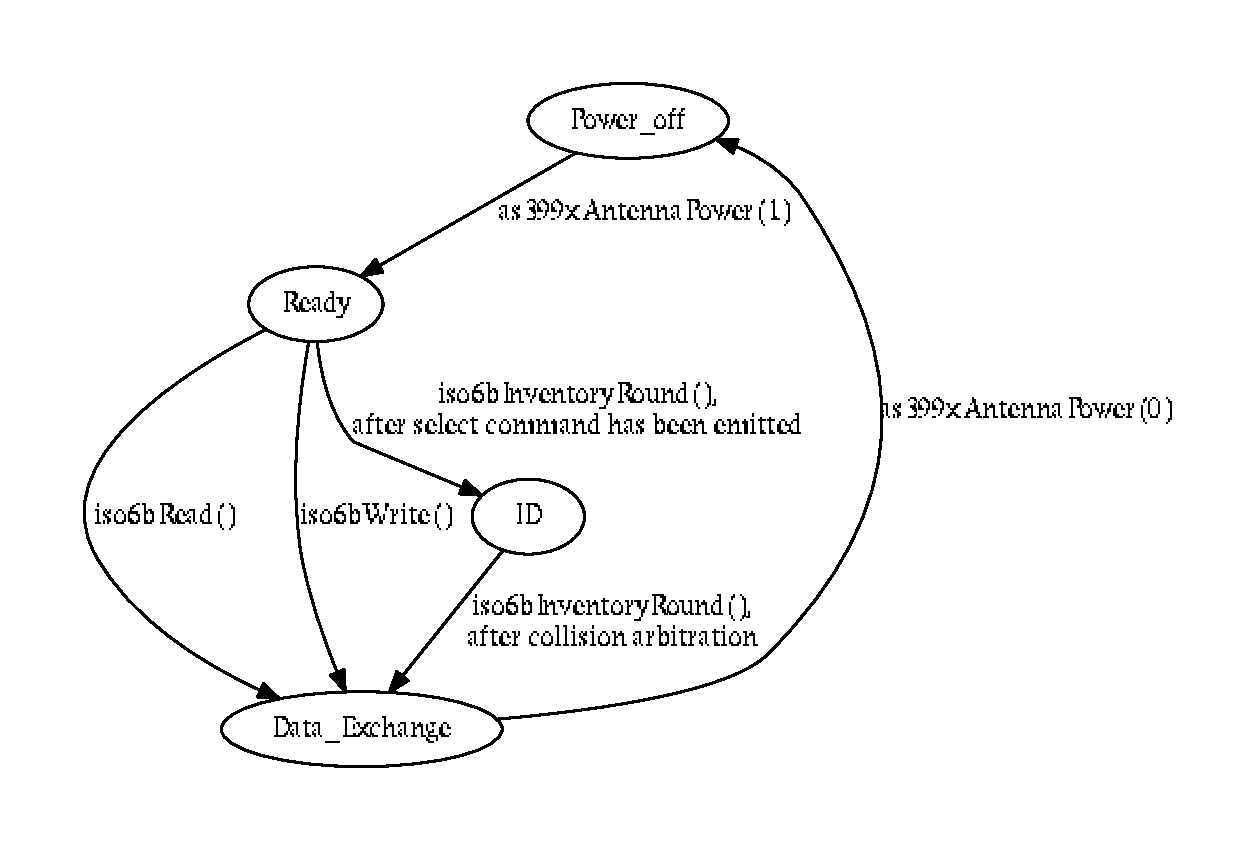
\includegraphics[width=\textwidth,height=\textheight/2,keepaspectratio=true]{dot_inline_dotgraph_3}}
\end{DoxyImageNoCaption}
\end{center}


It can be seen that iso6b\-Read() and iso6b\-Write() can be called without a prior inventory round. Both commands, however, do need the U\-I\-D of the tag which can only be determined by calling iso6b\-Inventory\-Round(). 

Definition in file {\bf iso6b.\-h}.


\section{main.\-c File Reference}
\label{main_8c}\index{main.\-c@{main.\-c}}
{\ttfamily \#include \char`\"{}as399x\-\_\-config.\-h\char`\"{}}\\*
{\ttfamily \#include \char`\"{}platform.\-h\char`\"{}}\\*
{\ttfamily \#include \char`\"{}c8051\-F340.\-h\char`\"{}}\\*
{\ttfamily \#include \char`\"{}uart.\-h\char`\"{}}\\*
{\ttfamily \#include \char`\"{}as399x\-\_\-public.\-h\char`\"{}}\\*
{\ttfamily \#include \char`\"{}as399x.\-h\char`\"{}}\\*
{\ttfamily \#include \char`\"{}as399x\-\_\-com.\-h\char`\"{}}\\*
{\ttfamily \#include \char`\"{}gen2.\-h\char`\"{}}\\*
{\ttfamily \#include \char`\"{}global.\-h\char`\"{}}\\*
{\ttfamily \#include \char`\"{}iso6b.\-h\char`\"{}}\\*
{\ttfamily \#include \char`\"{}tuner.\-h\char`\"{}}\\*
{\ttfamily \#include \char`\"{}timer.\-h\char`\"{}}\\*
{\ttfamily \#include \char`\"{}usb\-\_\-commands.\-h\char`\"{}}\\*
{\ttfamily \#include \char`\"{}F340\-\_\-\-Flash\-Primitives.\-h\char`\"{}}\\*
{\ttfamily \#include \char`\"{}F3xx\-\_\-\-U\-S\-B0\-\_\-\-Register.\-h\char`\"{}}\\*
{\ttfamily \#include \char`\"{}F3xx\-\_\-\-Blink\-\_\-\-Control.\-h\char`\"{}}\\*
{\ttfamily \#include \char`\"{}F3xx\-\_\-\-U\-S\-B0\-\_\-\-Interrupt\-Service\-Routine.\-h\char`\"{}}\\*
{\ttfamily \#include \char`\"{}F3xx\-\_\-\-U\-S\-B0\-\_\-\-Descriptor.\-h\char`\"{}}\\*
{\ttfamily \#include $<$math.\-h$>$}\\*
\subsection*{Functions}
\begin{DoxyCompactItemize}
\item 
int {\bf main} (void)
\end{DoxyCompactItemize}
\subsection*{Variables}
\begin{DoxyCompactItemize}
\item 
{\bf Tag} {\bf tags\-\_\-} [{\bf M\-A\-X\-T\-A\-G}]
\end{DoxyCompactItemize}


\subsection{Detailed Description}
System initialization and main loop. \begin{DoxyAuthor}{Author}
Ulrich Herrmann 
\end{DoxyAuthor}


Definition in file {\bf main.\-c}.



\subsection{Function Documentation}
\index{main.\-c@{main.\-c}!main@{main}}
\index{main@{main}!main.c@{main.\-c}}
\subsubsection[{main}]{\setlength{\rightskip}{0pt plus 5cm}int main (
\begin{DoxyParamCaption}
\item[{void}]{}
\end{DoxyParamCaption}
)}\label{main_8c_a840291bc02cba5474a4cb46a9b9566fe}
main function Initializes u\-Controller (System\-\_\-\-Init()) and A\-S399x (\doxyref{as399x\-Initialize()}{p.}{as399x_8c_a3bfe6fab3c61cffe7329b050c4523fc5}). Afterwards it enters main loop in which the commands received via U\-S\-B or U\-A\-R\-T are processed. 

Definition at line 199 of file main.\-c.



\subsection{Variable Documentation}
\index{main.\-c@{main.\-c}!tags\-\_\-@{tags\-\_\-}}
\index{tags\-\_\-@{tags\-\_\-}!main.c@{main.\-c}}
\subsubsection[{tags\-\_\-}]{\setlength{\rightskip}{0pt plus 5cm}{\bf Tag} tags\-\_\-[{\bf M\-A\-X\-T\-A\-G}]}\label{main_8c_a40526df6061b70feeef6f034db364b6e}
Array of Structures which stores all necessary Information about the Tags. 

Definition at line 82 of file usb\-\_\-commands.\-c.


\section{parallelinterface.\-c File Reference}
\label{parallelinterface_8c}\index{parallelinterface.\-c@{parallelinterface.\-c}}
{\ttfamily \#include \char`\"{}c8051\-F340.\-h\char`\"{}}\\*
{\ttfamily \#include \char`\"{}as399x\-\_\-config.\-h\char`\"{}}\\*
{\ttfamily \#include \char`\"{}platform.\-h\char`\"{}}\\*
{\ttfamily \#include \char`\"{}global.\-h\char`\"{}}\\*
{\ttfamily \#include \char`\"{}uart.\-h\char`\"{}}\\*
{\ttfamily \#include \char`\"{}timer.\-h\char`\"{}}\\*
{\ttfamily \#include \char`\"{}as399x\-\_\-com.\-h\char`\"{}}\\*
\subsection*{Macros}
\begin{DoxyCompactItemize}
\item 
\#define {\bf C\-L\-O\-C\-K}(x)~{\bf C\-L\-K\-P\-I\-N}=(x)
\item 
\#define {\bf D\-P\-O\-R\-T\-D\-I\-R\-W\-R}()~\{{\bf D\-P\-O\-R\-T\-D\-I\-R}(0x\-F\-F);\}
\item 
\#define {\bf D\-P\-O\-R\-T\-D\-I\-R\-R\-D}()~\{{\bf D\-P\-O\-R\-T\-D\-I\-R}(0x00); S\-E\-T\-O\-U\-T\-P\-O\-R\-T(0xff);\}
\item 
\#define {\bf G\-E\-T\-P\-O\-R\-T}()~{\bf D\-A\-T\-A\-I\-N\-P\-O\-R\-T}
\item 
\#define {\bf S\-T\-A\-R\-T\-C\-O\-N\-D\-I\-T\-I\-O\-N}()
\item 
\#define {\bf S\-T\-O\-P\-S\-G\-L}()
\item 
\#define {\bf S\-T\-O\-P\-C\-O\-N\-T}()
\item 
\#define {\bf S\-T\-O\-P\-D\-I\-R}()
\end{DoxyCompactItemize}
\subsection*{Functions}
\begin{DoxyCompactItemize}
\item 
void {\bf init\-Interface} (void)
\item 
void {\bf write\-Read\-A\-S399x} (const {\bf u8} $\ast$wbuf, {\bf u8} wlen, {\bf u8} $\ast$rbuf, {\bf u8} rlen, {\bf u8} stop\-Mode, {\bf u8} do\-Start)
\item 
void {\bf write\-Read\-A\-S399x\-Isr} (const {\bf u8} wbuf, {\bf u8} $\ast$rbuf)
\item 
void {\bf set\-Port\-Direct} ()
\item 
void {\bf set\-Port\-Normal} ()
\end{DoxyCompactItemize}


\subsection{Detailed Description}
Implementation of parallel interface communication with A\-S399x. The file provides functions to initialize the u\-Controller and the board for communication via the parallel interface with A\-S399x. The function \doxyref{write\-Read\-A\-S399x()}{p.}{as399x__com_8h_a66eee56b32bf33a739f1b0c3e7a57262} provides communication functionality. The function \doxyref{write\-Read\-A\-S399x\-Isr()}{p.}{as399x__com_8h_a35abe30a55f52f77670b663d2aef3d61} does the same, but is only called from the I\-S\-R. On the Si\-Labs u\-Controller a dedicated function for the I\-S\-R improves runtime performance (no reentrant function necessary). \par
For porting to another u\-Controller/board the functions in this file have to be adapted.

\begin{DoxyAuthor}{Author}
Ulrich Herrmann 

Bernhard Breinbauer 
\end{DoxyAuthor}


Definition in file {\bf parallelinterface.\-c}.



\subsection{Macro Definition Documentation}
\index{parallelinterface.\-c@{parallelinterface.\-c}!C\-L\-O\-C\-K@{C\-L\-O\-C\-K}}
\index{C\-L\-O\-C\-K@{C\-L\-O\-C\-K}!parallelinterface.c@{parallelinterface.\-c}}
\subsubsection[{C\-L\-O\-C\-K}]{\setlength{\rightskip}{0pt plus 5cm}\#define C\-L\-O\-C\-K(
\begin{DoxyParamCaption}
\item[{}]{x}
\end{DoxyParamCaption}
)~{\bf C\-L\-K\-P\-I\-N}=(x)}\label{parallelinterface_8c_a249b8376719383e8b8139e135101f1c4}
Macro for setting C\-L\-K pin 

Definition at line 49 of file parallelinterface.\-c.

\index{parallelinterface.\-c@{parallelinterface.\-c}!D\-P\-O\-R\-T\-D\-I\-R\-R\-D@{D\-P\-O\-R\-T\-D\-I\-R\-R\-D}}
\index{D\-P\-O\-R\-T\-D\-I\-R\-R\-D@{D\-P\-O\-R\-T\-D\-I\-R\-R\-D}!parallelinterface.c@{parallelinterface.\-c}}
\subsubsection[{D\-P\-O\-R\-T\-D\-I\-R\-R\-D}]{\setlength{\rightskip}{0pt plus 5cm}\#define D\-P\-O\-R\-T\-D\-I\-R\-R\-D(
\begin{DoxyParamCaption}
{}
\end{DoxyParamCaption}
)~\{{\bf D\-P\-O\-R\-T\-D\-I\-R}(0x00); S\-E\-T\-O\-U\-T\-P\-O\-R\-T(0xff);\}}\label{parallelinterface_8c_a7ef1777be40309789e715e367e1de577}
Macro change port direction to read 

Definition at line 55 of file parallelinterface.\-c.

\index{parallelinterface.\-c@{parallelinterface.\-c}!D\-P\-O\-R\-T\-D\-I\-R\-W\-R@{D\-P\-O\-R\-T\-D\-I\-R\-W\-R}}
\index{D\-P\-O\-R\-T\-D\-I\-R\-W\-R@{D\-P\-O\-R\-T\-D\-I\-R\-W\-R}!parallelinterface.c@{parallelinterface.\-c}}
\subsubsection[{D\-P\-O\-R\-T\-D\-I\-R\-W\-R}]{\setlength{\rightskip}{0pt plus 5cm}\#define D\-P\-O\-R\-T\-D\-I\-R\-W\-R(
\begin{DoxyParamCaption}
{}
\end{DoxyParamCaption}
)~\{{\bf D\-P\-O\-R\-T\-D\-I\-R}(0x\-F\-F);\}}\label{parallelinterface_8c_af7756551f319194bd0c597b1071cb8ac}
Macro change port direction to write 

Definition at line 52 of file parallelinterface.\-c.

\index{parallelinterface.\-c@{parallelinterface.\-c}!G\-E\-T\-P\-O\-R\-T@{G\-E\-T\-P\-O\-R\-T}}
\index{G\-E\-T\-P\-O\-R\-T@{G\-E\-T\-P\-O\-R\-T}!parallelinterface.c@{parallelinterface.\-c}}
\subsubsection[{G\-E\-T\-P\-O\-R\-T}]{\setlength{\rightskip}{0pt plus 5cm}\#define G\-E\-T\-P\-O\-R\-T(
\begin{DoxyParamCaption}
{}
\end{DoxyParamCaption}
)~{\bf D\-A\-T\-A\-I\-N\-P\-O\-R\-T}}\label{parallelinterface_8c_ae59a8ae0ad9dd1abe6d5bce9f579c672}
Macro read from data input port 

Definition at line 58 of file parallelinterface.\-c.

\index{parallelinterface.\-c@{parallelinterface.\-c}!S\-T\-A\-R\-T\-C\-O\-N\-D\-I\-T\-I\-O\-N@{S\-T\-A\-R\-T\-C\-O\-N\-D\-I\-T\-I\-O\-N}}
\index{S\-T\-A\-R\-T\-C\-O\-N\-D\-I\-T\-I\-O\-N@{S\-T\-A\-R\-T\-C\-O\-N\-D\-I\-T\-I\-O\-N}!parallelinterface.c@{parallelinterface.\-c}}
\subsubsection[{S\-T\-A\-R\-T\-C\-O\-N\-D\-I\-T\-I\-O\-N}]{\setlength{\rightskip}{0pt plus 5cm}\#define S\-T\-A\-R\-T\-C\-O\-N\-D\-I\-T\-I\-O\-N(
\begin{DoxyParamCaption}
{}
\end{DoxyParamCaption}
)}\label{parallelinterface_8c_a28297506ea74d55d37d04f6aea258096}
{\bfseries Value\-:}
\begin{DoxyCode}
\{CLOCK(LOW); SETOUTPORT(LOW); CLOCK(HIGH);\
                                   SETOUTPORT(0x80); NOP(); NOP(); CLOCK(LOW);\}
\end{DoxyCode}
Macro for protocol start condition 

Definition at line 61 of file parallelinterface.\-c.

\index{parallelinterface.\-c@{parallelinterface.\-c}!S\-T\-O\-P\-C\-O\-N\-T@{S\-T\-O\-P\-C\-O\-N\-T}}
\index{S\-T\-O\-P\-C\-O\-N\-T@{S\-T\-O\-P\-C\-O\-N\-T}!parallelinterface.c@{parallelinterface.\-c}}
\subsubsection[{S\-T\-O\-P\-C\-O\-N\-T}]{\setlength{\rightskip}{0pt plus 5cm}\#define S\-T\-O\-P\-C\-O\-N\-T(
\begin{DoxyParamCaption}
{}
\end{DoxyParamCaption}
)}\label{parallelinterface_8c_abdfdfa5aff3f112d5c020ba9ebe36358}
{\bfseries Value\-:}
\begin{DoxyCode}
\{CLOCK(LOW); SETOUTPORT(LOW); NOP(); SETOUTPORT(0x80);\
                                   NOP(); NOP(); SETOUTPORT(LOW);\}
\end{DoxyCode}
Macro for protocol continous stop condition 

Definition at line 67 of file parallelinterface.\-c.

\index{parallelinterface.\-c@{parallelinterface.\-c}!S\-T\-O\-P\-D\-I\-R@{S\-T\-O\-P\-D\-I\-R}}
\index{S\-T\-O\-P\-D\-I\-R@{S\-T\-O\-P\-D\-I\-R}!parallelinterface.c@{parallelinterface.\-c}}
\subsubsection[{S\-T\-O\-P\-D\-I\-R}]{\setlength{\rightskip}{0pt plus 5cm}\#define S\-T\-O\-P\-D\-I\-R(
\begin{DoxyParamCaption}
{}
\end{DoxyParamCaption}
)}\label{parallelinterface_8c_a896aa3bc9cfe4c9928d7716e8d018e51}
{\bfseries Value\-:}
\begin{DoxyCode}
\{SETOUTPORT(0x80); NOP(); NOP();\
                                   CLOCK(HIGH); NOP(); SETOUTPORT(LOW); NOP(); 
      CLOCK(LOW);\}
\end{DoxyCode}
Macro for ending the Direct mode 

Definition at line 70 of file parallelinterface.\-c.

\index{parallelinterface.\-c@{parallelinterface.\-c}!S\-T\-O\-P\-S\-G\-L@{S\-T\-O\-P\-S\-G\-L}}
\index{S\-T\-O\-P\-S\-G\-L@{S\-T\-O\-P\-S\-G\-L}!parallelinterface.c@{parallelinterface.\-c}}
\subsubsection[{S\-T\-O\-P\-S\-G\-L}]{\setlength{\rightskip}{0pt plus 5cm}\#define S\-T\-O\-P\-S\-G\-L(
\begin{DoxyParamCaption}
{}
\end{DoxyParamCaption}
)}\label{parallelinterface_8c_ab9dcc47b3f46dca4933d233a240bfcb9}
{\bfseries Value\-:}
\begin{DoxyCode}
\{SETOUTPORT(0x80); NOP();\
                                   CLOCK(HIGH); SETOUTPORT(LOW); CLOCK(LOW);\}
\end{DoxyCode}
Macro for protocol simple or single stop condition 

Definition at line 64 of file parallelinterface.\-c.



\subsection{Function Documentation}
\index{parallelinterface.\-c@{parallelinterface.\-c}!init\-Interface@{init\-Interface}}
\index{init\-Interface@{init\-Interface}!parallelinterface.c@{parallelinterface.\-c}}
\subsubsection[{init\-Interface}]{\setlength{\rightskip}{0pt plus 5cm}void init\-Interface (
\begin{DoxyParamCaption}
\item[{void}]{}
\end{DoxyParamCaption}
)}\label{parallelinterface_8c_a6305d3b6e2bbab54bca14afc97db3c5c}
This function initializes u\-Controller/board for comunication with the A\-S399x.

This function does not take or return a parameter. 

Definition at line 113 of file parallelinterface.\-c.

\index{parallelinterface.\-c@{parallelinterface.\-c}!set\-Port\-Direct@{set\-Port\-Direct}}
\index{set\-Port\-Direct@{set\-Port\-Direct}!parallelinterface.c@{parallelinterface.\-c}}
\subsubsection[{set\-Port\-Direct}]{\setlength{\rightskip}{0pt plus 5cm}void set\-Port\-Direct (
\begin{DoxyParamCaption}
{}
\end{DoxyParamCaption}
)}\label{parallelinterface_8c_aeeadd66a92ac517951a886b62eb1fb75}
This function sets the interface to the A\-S399\-X for accessing it via direct mode. \doxyref{I\-O3()}{p.}{platform_8h_adc9689bf9fd884c1d840a3aa947a0a39} macro needs to be used to generate T\-X signals 

Definition at line 203 of file parallelinterface.\-c.

\index{parallelinterface.\-c@{parallelinterface.\-c}!set\-Port\-Normal@{set\-Port\-Normal}}
\index{set\-Port\-Normal@{set\-Port\-Normal}!parallelinterface.c@{parallelinterface.\-c}}
\subsubsection[{set\-Port\-Normal}]{\setlength{\rightskip}{0pt plus 5cm}void set\-Port\-Normal (
\begin{DoxyParamCaption}
{}
\end{DoxyParamCaption}
)}\label{parallelinterface_8c_a48f08cfa3d7253dcd2520cad24e18e41}
This function sets the interface to the A\-S399\-X for accessing it via normal (parallel) mode using \doxyref{write\-Read\-A\-S399x()}{p.}{as399x__com_8h_a66eee56b32bf33a739f1b0c3e7a57262} 

Definition at line 210 of file parallelinterface.\-c.

\index{parallelinterface.\-c@{parallelinterface.\-c}!write\-Read\-A\-S399x@{write\-Read\-A\-S399x}}
\index{write\-Read\-A\-S399x@{write\-Read\-A\-S399x}!parallelinterface.c@{parallelinterface.\-c}}
\subsubsection[{write\-Read\-A\-S399x}]{\setlength{\rightskip}{0pt plus 5cm}void write\-Read\-A\-S399x (
\begin{DoxyParamCaption}
\item[{const {\bf u8} $\ast$}]{wbuf, }
\item[{{\bf u8}}]{wlen, }
\item[{{\bf u8} $\ast$}]{rbuf, }
\item[{{\bf u8}}]{rlen, }
\item[{{\bf u8}}]{stop\-Mode, }
\item[{{\bf u8}}]{do\-Start}
\end{DoxyParamCaption}
)}\label{parallelinterface_8c_a66eee56b32bf33a739f1b0c3e7a57262}
This function talks with the A\-S399x chip. 

Definition at line 129 of file parallelinterface.\-c.

\index{parallelinterface.\-c@{parallelinterface.\-c}!write\-Read\-A\-S399x\-Isr@{write\-Read\-A\-S399x\-Isr}}
\index{write\-Read\-A\-S399x\-Isr@{write\-Read\-A\-S399x\-Isr}!parallelinterface.c@{parallelinterface.\-c}}
\subsubsection[{write\-Read\-A\-S399x\-Isr}]{\setlength{\rightskip}{0pt plus 5cm}void write\-Read\-A\-S399x\-Isr (
\begin{DoxyParamCaption}
\item[{const {\bf u8}}]{wbuf, }
\item[{{\bf u8} $\ast$}]{rbuf}
\end{DoxyParamCaption}
)}\label{parallelinterface_8c_a35abe30a55f52f77670b663d2aef3d61}
This function talks with the A\-S399x chip from I\-S\-R. 

Definition at line 166 of file parallelinterface.\-c.


\section{platform.\-h File Reference}
\label{platform_8h}\index{platform.\-h@{platform.\-h}}
{\ttfamily \#include \char`\"{}c8051\-F340.\-h\char`\"{}}\\*
{\ttfamily \#include $<$intrins.\-h$>$}\\*
{\ttfamily \#include \char`\"{}global.\-h\char`\"{}}\\*
{\ttfamily \#include \char`\"{}as399x\-\_\-config.\-h\char`\"{}}\\*
\subsection*{Macros}
\begin{DoxyCompactItemize}
\item 
\#define {\bf E\-N\-E\-X\-T\-I\-R\-Q}()~\{E\-X0 = 1;\}
\item 
\#define {\bf D\-I\-S\-E\-X\-T\-I\-R\-Q}()~E\-X0 = 0
\item 
\#define {\bf S\-E\-T\-O\-U\-T\-P\-O\-R\-T}(x)~{\bf D\-A\-T\-A\-O\-U\-T\-P\-O\-R\-T}=(x)
\item 
\#define {\bf D\-P\-O\-R\-T\-D\-I\-R}(x)~P1\-M\-D\-O\-U\-T=(x);
\item 
\#define {\bf E\-N}(x)~{\bf E\-N\-A\-B\-L\-E}=(x)
\item 
\#define {\bf E\-N\-\_\-\-L\-D\-O\-\_\-\-A\-S399x}(x)~;
\item 
\#define {\bf D\-C\-D\-C}(x)~{\bf D\-C\-D\-C\-P\-I\-N}=(x)
\item 
\#define {\bf E\-N\-\_\-\-P\-A}(x)~{\bf E\-N\-\_\-\-P\-A\-P\-I\-N}=(x)
\item 
\#define {\bf I\-O2}(x)~{\bf I\-O2\-P\-I\-N}=(x)
\item 
\#define {\bf I\-O3}(x)~{\bf I\-O3\-P\-I\-N}=(x)
\item 
\#define {\bf I\-O4}(x)~P1\-\_\-4=(x)
\item 
\#define {\bf I\-R\-Q\-P\-I\-N}~P0\-\_\-3
\item 
\#define {\bf L\-E\-D1\-P\-I\-N}~P2\-\_\-2
\item 
\#define {\bf E\-N\-A\-B\-L\-E}~P2\-\_\-1
\item 
\#define {\bf D\-C\-D\-C\-P\-I\-N}~P0\-\_\-2
\item 
\#define {\bf E\-N\-\_\-\-P\-A\-P\-I\-N}~P3\-\_\-0
\item 
\#define {\bf I\-O3\-P\-I\-N}~P1\-\_\-3
\item 
\#define {\bf I\-O2\-P\-I\-N}~P1\-\_\-2
\item 
\#define {\bf I\-O5\-P\-I\-N}~P1\-\_\-5
\item 
\#define {\bf I\-O6\-P\-I\-N}~P1\-\_\-6
\item 
\#define {\bf D\-A\-T\-A\-O\-U\-T\-P\-O\-R\-T}~P1
\item 
\#define {\bf D\-A\-T\-A\-I\-N\-P\-O\-R\-T}~P1
\item 
\#define {\bf C\-L\-K\-P\-I\-N}~P2\-\_\-0
\item 
\#define {\bf S\-Y\-S\-C\-L\-K\-I\-N}~P0\-\_\-7
\end{DoxyCompactItemize}


\subsection{Detailed Description}
This file provides platform (board) specific macros and declarations. \begin{DoxyAuthor}{Author}
B. Breinbauer
\end{DoxyAuthor}
Contains configuration macros which are used throughout the code base, to enable/disable board specific features. 

Definition in file {\bf platform.\-h}.



\subsection{Macro Definition Documentation}
\index{platform.\-h@{platform.\-h}!C\-L\-K\-P\-I\-N@{C\-L\-K\-P\-I\-N}}
\index{C\-L\-K\-P\-I\-N@{C\-L\-K\-P\-I\-N}!platform.h@{platform.\-h}}
\subsubsection[{C\-L\-K\-P\-I\-N}]{\setlength{\rightskip}{0pt plus 5cm}\#define C\-L\-K\-P\-I\-N~P2\-\_\-0}\label{platform_8h_a377f8bedbca96a219ff5a78bf54f8e1e}
Definition for the clk pin of the for the parallel interface 

Definition at line 175 of file platform.\-h.

\index{platform.\-h@{platform.\-h}!D\-A\-T\-A\-I\-N\-P\-O\-R\-T@{D\-A\-T\-A\-I\-N\-P\-O\-R\-T}}
\index{D\-A\-T\-A\-I\-N\-P\-O\-R\-T@{D\-A\-T\-A\-I\-N\-P\-O\-R\-T}!platform.h@{platform.\-h}}
\subsubsection[{D\-A\-T\-A\-I\-N\-P\-O\-R\-T}]{\setlength{\rightskip}{0pt plus 5cm}\#define D\-A\-T\-A\-I\-N\-P\-O\-R\-T~P1}\label{platform_8h_a2c3ecf3627d7fc3f40926e983ee16b2a}
Definition for the 8 bit (parallel) data input port 

Definition at line 173 of file platform.\-h.

\index{platform.\-h@{platform.\-h}!D\-A\-T\-A\-O\-U\-T\-P\-O\-R\-T@{D\-A\-T\-A\-O\-U\-T\-P\-O\-R\-T}}
\index{D\-A\-T\-A\-O\-U\-T\-P\-O\-R\-T@{D\-A\-T\-A\-O\-U\-T\-P\-O\-R\-T}!platform.h@{platform.\-h}}
\subsubsection[{D\-A\-T\-A\-O\-U\-T\-P\-O\-R\-T}]{\setlength{\rightskip}{0pt plus 5cm}\#define D\-A\-T\-A\-O\-U\-T\-P\-O\-R\-T~P1}\label{platform_8h_ad8c9bdaf4b39e7a77066c55b7a25a5a5}
Definition for the 8 bit (parallel) data outport 

Definition at line 171 of file platform.\-h.

\index{platform.\-h@{platform.\-h}!D\-C\-D\-C@{D\-C\-D\-C}}
\index{D\-C\-D\-C@{D\-C\-D\-C}!platform.h@{platform.\-h}}
\subsubsection[{D\-C\-D\-C}]{\setlength{\rightskip}{0pt plus 5cm}\#define D\-C\-D\-C(
\begin{DoxyParamCaption}
\item[{}]{x}
\end{DoxyParamCaption}
)~{\bf D\-C\-D\-C\-P\-I\-N}=(x)}\label{platform_8h_a53843008bd133c33da96bea584ff61d2}
Macro for setting D\-C\-D\-C on/off 

Definition at line 68 of file platform.\-h.

\index{platform.\-h@{platform.\-h}!D\-C\-D\-C\-P\-I\-N@{D\-C\-D\-C\-P\-I\-N}}
\index{D\-C\-D\-C\-P\-I\-N@{D\-C\-D\-C\-P\-I\-N}!platform.h@{platform.\-h}}
\subsubsection[{D\-C\-D\-C\-P\-I\-N}]{\setlength{\rightskip}{0pt plus 5cm}\#define D\-C\-D\-C\-P\-I\-N~P0\-\_\-2}\label{platform_8h_ae83f57c95654d7adf6e7abdd350436d3}
Definition for the D\-C\-D\-C enable pin 

Definition at line 147 of file platform.\-h.

\index{platform.\-h@{platform.\-h}!D\-I\-S\-E\-X\-T\-I\-R\-Q@{D\-I\-S\-E\-X\-T\-I\-R\-Q}}
\index{D\-I\-S\-E\-X\-T\-I\-R\-Q@{D\-I\-S\-E\-X\-T\-I\-R\-Q}!platform.h@{platform.\-h}}
\subsubsection[{D\-I\-S\-E\-X\-T\-I\-R\-Q}]{\setlength{\rightskip}{0pt plus 5cm}\#define D\-I\-S\-E\-X\-T\-I\-R\-Q(
\begin{DoxyParamCaption}
{}
\end{DoxyParamCaption}
)~E\-X0 = 0}\label{platform_8h_a2ecf545f9456911955f2b3bcc2884ff1}
Macro for disable external I\-R\-Q 

Definition at line 44 of file platform.\-h.

\index{platform.\-h@{platform.\-h}!D\-P\-O\-R\-T\-D\-I\-R@{D\-P\-O\-R\-T\-D\-I\-R}}
\index{D\-P\-O\-R\-T\-D\-I\-R@{D\-P\-O\-R\-T\-D\-I\-R}!platform.h@{platform.\-h}}
\subsubsection[{D\-P\-O\-R\-T\-D\-I\-R}]{\setlength{\rightskip}{0pt plus 5cm}\#define D\-P\-O\-R\-T\-D\-I\-R(
\begin{DoxyParamCaption}
\item[{}]{x}
\end{DoxyParamCaption}
)~P1\-M\-D\-O\-U\-T=(x);}\label{platform_8h_ae61be8bdbf5eb42a84a29929e2793d62}
Macro change port direction 

Definition at line 50 of file platform.\-h.

\index{platform.\-h@{platform.\-h}!E\-N@{E\-N}}
\index{E\-N@{E\-N}!platform.h@{platform.\-h}}
\subsubsection[{E\-N}]{\setlength{\rightskip}{0pt plus 5cm}\#define E\-N(
\begin{DoxyParamCaption}
\item[{}]{x}
\end{DoxyParamCaption}
)~{\bf E\-N\-A\-B\-L\-E}=(x)}\label{platform_8h_aa28a3e21fdb1bf90626afd179b26756b}
Macro for setting enable pin 

Definition at line 57 of file platform.\-h.

\index{platform.\-h@{platform.\-h}!E\-N\-\_\-\-L\-D\-O\-\_\-\-A\-S399x@{E\-N\-\_\-\-L\-D\-O\-\_\-\-A\-S399x}}
\index{E\-N\-\_\-\-L\-D\-O\-\_\-\-A\-S399x@{E\-N\-\_\-\-L\-D\-O\-\_\-\-A\-S399x}!platform.h@{platform.\-h}}
\subsubsection[{E\-N\-\_\-\-L\-D\-O\-\_\-\-A\-S399x}]{\setlength{\rightskip}{0pt plus 5cm}\#define E\-N\-\_\-\-L\-D\-O\-\_\-\-A\-S399x(
\begin{DoxyParamCaption}
\item[{}]{x}
\end{DoxyParamCaption}
)~;}\label{platform_8h_a3b7b6224a9fdb6fbb664799a7e63a558}
Macro for enabling L\-D\-O which powers A\-S399x (not available on all boards) 

Definition at line 64 of file platform.\-h.

\index{platform.\-h@{platform.\-h}!E\-N\-\_\-\-P\-A@{E\-N\-\_\-\-P\-A}}
\index{E\-N\-\_\-\-P\-A@{E\-N\-\_\-\-P\-A}!platform.h@{platform.\-h}}
\subsubsection[{E\-N\-\_\-\-P\-A}]{\setlength{\rightskip}{0pt plus 5cm}\#define E\-N\-\_\-\-P\-A(
\begin{DoxyParamCaption}
\item[{}]{x}
\end{DoxyParamCaption}
)~{\bf E\-N\-\_\-\-P\-A\-P\-I\-N}=(x)}\label{platform_8h_aa539ee5694a63294bddca2c47cfa0234}
Macro for setting P\-A on/off 

Definition at line 71 of file platform.\-h.

\index{platform.\-h@{platform.\-h}!E\-N\-\_\-\-P\-A\-P\-I\-N@{E\-N\-\_\-\-P\-A\-P\-I\-N}}
\index{E\-N\-\_\-\-P\-A\-P\-I\-N@{E\-N\-\_\-\-P\-A\-P\-I\-N}!platform.h@{platform.\-h}}
\subsubsection[{E\-N\-\_\-\-P\-A\-P\-I\-N}]{\setlength{\rightskip}{0pt plus 5cm}\#define E\-N\-\_\-\-P\-A\-P\-I\-N~P3\-\_\-0}\label{platform_8h_ab6942a2866ad6f01ed8c9ce1e493d27a}
Definition for the P\-A enable Pin 

Definition at line 149 of file platform.\-h.

\index{platform.\-h@{platform.\-h}!E\-N\-A\-B\-L\-E@{E\-N\-A\-B\-L\-E}}
\index{E\-N\-A\-B\-L\-E@{E\-N\-A\-B\-L\-E}!platform.h@{platform.\-h}}
\subsubsection[{E\-N\-A\-B\-L\-E}]{\setlength{\rightskip}{0pt plus 5cm}\#define E\-N\-A\-B\-L\-E~P2\-\_\-1}\label{platform_8h_a514ad415fb6125ba296793df7d1a468a}
Definition for the enable pin 

Definition at line 145 of file platform.\-h.

\index{platform.\-h@{platform.\-h}!E\-N\-E\-X\-T\-I\-R\-Q@{E\-N\-E\-X\-T\-I\-R\-Q}}
\index{E\-N\-E\-X\-T\-I\-R\-Q@{E\-N\-E\-X\-T\-I\-R\-Q}!platform.h@{platform.\-h}}
\subsubsection[{E\-N\-E\-X\-T\-I\-R\-Q}]{\setlength{\rightskip}{0pt plus 5cm}\#define E\-N\-E\-X\-T\-I\-R\-Q(
\begin{DoxyParamCaption}
{}
\end{DoxyParamCaption}
)~\{E\-X0 = 1;\}}\label{platform_8h_a034e8f1d1358c558a547b73703363c42}
Macro for enable external I\-R\-Q 

Definition at line 41 of file platform.\-h.

\index{platform.\-h@{platform.\-h}!I\-O2@{I\-O2}}
\index{I\-O2@{I\-O2}!platform.h@{platform.\-h}}
\subsubsection[{I\-O2}]{\setlength{\rightskip}{0pt plus 5cm}\#define I\-O2(
\begin{DoxyParamCaption}
\item[{}]{x}
\end{DoxyParamCaption}
)~{\bf I\-O2\-P\-I\-N}=(x)}\label{platform_8h_a20ce1e804f77640c9fcde159e7e5fb9d}
Macro for setting I\-O2 pin, for direct mode 

Definition at line 74 of file platform.\-h.

\index{platform.\-h@{platform.\-h}!I\-O2\-P\-I\-N@{I\-O2\-P\-I\-N}}
\index{I\-O2\-P\-I\-N@{I\-O2\-P\-I\-N}!platform.h@{platform.\-h}}
\subsubsection[{I\-O2\-P\-I\-N}]{\setlength{\rightskip}{0pt plus 5cm}\#define I\-O2\-P\-I\-N~P1\-\_\-2}\label{platform_8h_a0e4ec8f0c54b4c290bd14d4fbce60967}
Definition for the Direct data mode Pin 

Definition at line 153 of file platform.\-h.

\index{platform.\-h@{platform.\-h}!I\-O3@{I\-O3}}
\index{I\-O3@{I\-O3}!platform.h@{platform.\-h}}
\subsubsection[{I\-O3}]{\setlength{\rightskip}{0pt plus 5cm}\#define I\-O3(
\begin{DoxyParamCaption}
\item[{}]{x}
\end{DoxyParamCaption}
)~{\bf I\-O3\-P\-I\-N}=(x)}\label{platform_8h_adc9689bf9fd884c1d840a3aa947a0a39}
Macro for setting I\-O3 pin, for direct mode 

Definition at line 77 of file platform.\-h.

\index{platform.\-h@{platform.\-h}!I\-O3\-P\-I\-N@{I\-O3\-P\-I\-N}}
\index{I\-O3\-P\-I\-N@{I\-O3\-P\-I\-N}!platform.h@{platform.\-h}}
\subsubsection[{I\-O3\-P\-I\-N}]{\setlength{\rightskip}{0pt plus 5cm}\#define I\-O3\-P\-I\-N~P1\-\_\-3}\label{platform_8h_a589bdd59b3b6aea7eeed055b149c063c}
Definition for the Direct data mode Pin 

Definition at line 151 of file platform.\-h.

\index{platform.\-h@{platform.\-h}!I\-O4@{I\-O4}}
\index{I\-O4@{I\-O4}!platform.h@{platform.\-h}}
\subsubsection[{I\-O4}]{\setlength{\rightskip}{0pt plus 5cm}\#define I\-O4(
\begin{DoxyParamCaption}
\item[{}]{x}
\end{DoxyParamCaption}
)~P1\-\_\-4=(x)}\label{platform_8h_a3abd90ec4a4016ea37edb6d67d6daf31}
Macro for setting I\-O4 pin, serial enable line 

Definition at line 85 of file platform.\-h.

\index{platform.\-h@{platform.\-h}!I\-O5\-P\-I\-N@{I\-O5\-P\-I\-N}}
\index{I\-O5\-P\-I\-N@{I\-O5\-P\-I\-N}!platform.h@{platform.\-h}}
\subsubsection[{I\-O5\-P\-I\-N}]{\setlength{\rightskip}{0pt plus 5cm}\#define I\-O5\-P\-I\-N~P1\-\_\-5}\label{platform_8h_af2584caa41b0a6851dba98169a6edaa6}
Definition for the Direct mode data bitclock Pin 

Definition at line 155 of file platform.\-h.

\index{platform.\-h@{platform.\-h}!I\-O6\-P\-I\-N@{I\-O6\-P\-I\-N}}
\index{I\-O6\-P\-I\-N@{I\-O6\-P\-I\-N}!platform.h@{platform.\-h}}
\subsubsection[{I\-O6\-P\-I\-N}]{\setlength{\rightskip}{0pt plus 5cm}\#define I\-O6\-P\-I\-N~P1\-\_\-6}\label{platform_8h_a6a776b13fcdfe2b027cd9d84f180a791}
Definition for the Direct mode data Pin 

Definition at line 160 of file platform.\-h.

\index{platform.\-h@{platform.\-h}!I\-R\-Q\-P\-I\-N@{I\-R\-Q\-P\-I\-N}}
\index{I\-R\-Q\-P\-I\-N@{I\-R\-Q\-P\-I\-N}!platform.h@{platform.\-h}}
\subsubsection[{I\-R\-Q\-P\-I\-N}]{\setlength{\rightskip}{0pt plus 5cm}\#define I\-R\-Q\-P\-I\-N~P0\-\_\-3}\label{platform_8h_a02b244499426b898fdc751e44f688f19}
Definition for the external I\-R\-Q pin 

Definition at line 91 of file platform.\-h.

\index{platform.\-h@{platform.\-h}!L\-E\-D1\-P\-I\-N@{L\-E\-D1\-P\-I\-N}}
\index{L\-E\-D1\-P\-I\-N@{L\-E\-D1\-P\-I\-N}!platform.h@{platform.\-h}}
\subsubsection[{L\-E\-D1\-P\-I\-N}]{\setlength{\rightskip}{0pt plus 5cm}\#define L\-E\-D1\-P\-I\-N~P2\-\_\-2}\label{platform_8h_a04d7aaffbb7b5afaf49acf8a3a39e33a}
Definition for the L\-E\-D 1 (L\-E\-O) 

Definition at line 98 of file platform.\-h.

\index{platform.\-h@{platform.\-h}!S\-E\-T\-O\-U\-T\-P\-O\-R\-T@{S\-E\-T\-O\-U\-T\-P\-O\-R\-T}}
\index{S\-E\-T\-O\-U\-T\-P\-O\-R\-T@{S\-E\-T\-O\-U\-T\-P\-O\-R\-T}!platform.h@{platform.\-h}}
\subsubsection[{S\-E\-T\-O\-U\-T\-P\-O\-R\-T}]{\setlength{\rightskip}{0pt plus 5cm}\#define S\-E\-T\-O\-U\-T\-P\-O\-R\-T(
\begin{DoxyParamCaption}
\item[{}]{x}
\end{DoxyParamCaption}
)~{\bf D\-A\-T\-A\-O\-U\-T\-P\-O\-R\-T}=(x)}\label{platform_8h_ae6f4781761dd3b6dd1254a1c94fdcc9b}
Macro setting data output port 

Definition at line 47 of file platform.\-h.

\index{platform.\-h@{platform.\-h}!S\-Y\-S\-C\-L\-K\-I\-N@{S\-Y\-S\-C\-L\-K\-I\-N}}
\index{S\-Y\-S\-C\-L\-K\-I\-N@{S\-Y\-S\-C\-L\-K\-I\-N}!platform.h@{platform.\-h}}
\subsubsection[{S\-Y\-S\-C\-L\-K\-I\-N}]{\setlength{\rightskip}{0pt plus 5cm}\#define S\-Y\-S\-C\-L\-K\-I\-N~P0\-\_\-7}\label{platform_8h_ac4612fb169d77d829f4b8ae0dc6a57c1}
Definition for the u\-C C\-L\-K Input pin 

Definition at line 177 of file platform.\-h.


\section{serialinterface.\-c File Reference}
\label{serialinterface_8c}\index{serialinterface.\-c@{serialinterface.\-c}}
{\ttfamily \#include \char`\"{}c8051\-F340.\-h\char`\"{}}\\*
{\ttfamily \#include \char`\"{}as399x\-\_\-config.\-h\char`\"{}}\\*
{\ttfamily \#include \char`\"{}platform.\-h\char`\"{}}\\*
{\ttfamily \#include \char`\"{}global.\-h\char`\"{}}\\*
{\ttfamily \#include \char`\"{}uart.\-h\char`\"{}}\\*
{\ttfamily \#include \char`\"{}timer.\-h\char`\"{}}\\*
{\ttfamily \#include \char`\"{}as399x\-\_\-com.\-h\char`\"{}}\\*
\subsection*{Functions}
\begin{DoxyCompactItemize}
\item 
void {\bf init\-Interface} (void)
\item 
void {\bf write\-Read\-A\-S399x} (const {\bf u8} $\ast$wbuf, {\bf u8} wlen, {\bf u8} $\ast$rbuf, {\bf u8} rlen, {\bf u8} stop\-Mode, {\bf u8} do\-Start)
\item 
void {\bf write\-Read\-A\-S399x\-Isr} (const {\bf u8} wbuf, {\bf u8} $\ast$rbuf)
\item 
void {\bf set\-Port\-Direct} ()
\item 
void {\bf set\-Port\-Normal} ()
\end{DoxyCompactItemize}


\subsection{Detailed Description}
Implementation of serial interface communication with A\-S399x. The file provides functions to initialize the u\-Controller and the board for S\-P\-I communication with A\-S399x. The function \doxyref{write\-Read\-A\-S399x()}{p.}{as399x__com_8h_a66eee56b32bf33a739f1b0c3e7a57262} provides communication functionality. The function \doxyref{write\-Read\-A\-S399x\-Isr()}{p.}{as399x__com_8h_a35abe30a55f52f77670b663d2aef3d61} does the same, but is only called from the I\-S\-R. On the Si\-Labs u\-Controller a dedicated function for the I\-S\-R improves runtime performance (no reentrant function necessary). \par
For porting to another u\-Controller/board the functions in this file have to be adapted. \par
\par
For serial communication on L\-E\-O boards a patch is required. The patch does the following\-: 
\begin{DoxyItemize}
\item P0\-\_\-0(\-S\-P\-I S\-C\-K) -\/ P2\-\_\-0 -\/ \doxyref{C\-L\-K(\-A\-S399\-X)}{p.}{global_8h_a4b355291fe6b8ba8e167ab0faa862e45} 
\item P0\-\_\-1(\-S\-P\-I M\-I\-S\-O) -\/ P1\-\_\-6 -\/ I\-O6(\-A\-S399\-X) 
\item P0\-\_\-2(\-S\-P\-I M\-O\-S\-I) -\/ P1\-\_\-7 -\/ I\-O7(\-A\-S399\-X) 
\end{DoxyItemize}Therefore P1\-\_\-6, P1\-\_\-7, P2\-\_\-0, P0\-\_\-1 need to be configured input (open drain). And P0\-\_\-0 and P0\-\_\-2 need to be configured output (push pull).

\begin{DoxyAuthor}{Author}
Ulrich Herrmann 

Bernhard Breinbauer 
\end{DoxyAuthor}


Definition in file {\bf serialinterface.\-c}.



\subsection{Function Documentation}
\index{serialinterface.\-c@{serialinterface.\-c}!init\-Interface@{init\-Interface}}
\index{init\-Interface@{init\-Interface}!serialinterface.c@{serialinterface.\-c}}
\subsubsection[{init\-Interface}]{\setlength{\rightskip}{0pt plus 5cm}void init\-Interface (
\begin{DoxyParamCaption}
\item[{void}]{}
\end{DoxyParamCaption}
)}\label{serialinterface_8c_a6305d3b6e2bbab54bca14afc97db3c5c}
This function initializes the in/out ports of the controller for communication with A\-S399x via S\-P\-I. \par
This function has to be adapted for new boards/controllers/... 

Definition at line 75 of file serialinterface.\-c.

\index{serialinterface.\-c@{serialinterface.\-c}!set\-Port\-Direct@{set\-Port\-Direct}}
\index{set\-Port\-Direct@{set\-Port\-Direct}!serialinterface.c@{serialinterface.\-c}}
\subsubsection[{set\-Port\-Direct}]{\setlength{\rightskip}{0pt plus 5cm}void set\-Port\-Direct (
\begin{DoxyParamCaption}
{}
\end{DoxyParamCaption}
)}\label{serialinterface_8c_aeeadd66a92ac517951a886b62eb1fb75}
This function sets the interface to the A\-S399\-X for accessing it via direct mode. \doxyref{I\-O3()}{p.}{platform_8h_adc9689bf9fd884c1d840a3aa947a0a39} macro needs to be used to generate T\-X signals 

Definition at line 199 of file serialinterface.\-c.

\index{serialinterface.\-c@{serialinterface.\-c}!set\-Port\-Normal@{set\-Port\-Normal}}
\index{set\-Port\-Normal@{set\-Port\-Normal}!serialinterface.c@{serialinterface.\-c}}
\subsubsection[{set\-Port\-Normal}]{\setlength{\rightskip}{0pt plus 5cm}void set\-Port\-Normal (
\begin{DoxyParamCaption}
{}
\end{DoxyParamCaption}
)}\label{serialinterface_8c_a48f08cfa3d7253dcd2520cad24e18e41}
This function sets the interface to the A\-S399\-X for accessing it via normal (parallel) mode using \doxyref{write\-Read\-A\-S399x()}{p.}{as399x__com_8h_a66eee56b32bf33a739f1b0c3e7a57262} 

Definition at line 204 of file serialinterface.\-c.

\index{serialinterface.\-c@{serialinterface.\-c}!write\-Read\-A\-S399x@{write\-Read\-A\-S399x}}
\index{write\-Read\-A\-S399x@{write\-Read\-A\-S399x}!serialinterface.c@{serialinterface.\-c}}
\subsubsection[{write\-Read\-A\-S399x}]{\setlength{\rightskip}{0pt plus 5cm}void write\-Read\-A\-S399x (
\begin{DoxyParamCaption}
\item[{const {\bf u8} $\ast$}]{wbuf, }
\item[{{\bf u8}}]{wlen, }
\item[{{\bf u8} $\ast$}]{rbuf, }
\item[{{\bf u8}}]{rlen, }
\item[{{\bf u8}}]{stop\-Mode, }
\item[{{\bf u8}}]{do\-Start}
\end{DoxyParamCaption}
)}\label{serialinterface_8c_a66eee56b32bf33a739f1b0c3e7a57262}
This function talks with the A\-S399x chip. 

Definition at line 153 of file serialinterface.\-c.

\index{serialinterface.\-c@{serialinterface.\-c}!write\-Read\-A\-S399x\-Isr@{write\-Read\-A\-S399x\-Isr}}
\index{write\-Read\-A\-S399x\-Isr@{write\-Read\-A\-S399x\-Isr}!serialinterface.c@{serialinterface.\-c}}
\subsubsection[{write\-Read\-A\-S399x\-Isr}]{\setlength{\rightskip}{0pt plus 5cm}void write\-Read\-A\-S399x\-Isr (
\begin{DoxyParamCaption}
\item[{const {\bf u8}}]{wbuf, }
\item[{{\bf u8} $\ast$}]{rbuf}
\end{DoxyParamCaption}
)}\label{serialinterface_8c_a35abe30a55f52f77670b663d2aef3d61}
This function talks with the A\-S399x chip from I\-S\-R. 

Definition at line 180 of file serialinterface.\-c.


\section{timer.\-c File Reference}
\label{timer_8c}\index{timer.\-c@{timer.\-c}}
{\ttfamily \#include \char`\"{}c8051\-F340.\-h\char`\"{}}\\*
{\ttfamily \#include \char`\"{}as399x\-\_\-config.\-h\char`\"{}}\\*
{\ttfamily \#include \char`\"{}timer.\-h\char`\"{}}\\*
{\ttfamily \#include \char`\"{}global.\-h\char`\"{}}\\*
\subsection*{Functions}
\begin{DoxyCompactItemize}
\item 
void {\bf mdelay} (u16 ms)
\item 
void {\bf timer\-Start\-\_\-us} (u16 us)
\item 
void {\bf udelay} (u16 us)
\item 
void {\bf timer\-Start\-Measure} ()
\item 
u16 {\bf timer\-Measure\-\_\-slow\-Ticks} ()
\end{DoxyCompactItemize}


\subsection{Detailed Description}
This file includes all functionality to use some hardware timers. \begin{DoxyAuthor}{Author}
Ulrich Herrmann 
\end{DoxyAuthor}


Definition in file {\bf timer.\-c}.



\subsection{Function Documentation}
\index{timer.\-c@{timer.\-c}!mdelay@{mdelay}}
\index{mdelay@{mdelay}!timer.c@{timer.\-c}}
\subsubsection[{mdelay}]{\setlength{\rightskip}{0pt plus 5cm}void mdelay (
\begin{DoxyParamCaption}
\item[{u16}]{ms}
\end{DoxyParamCaption}
)}\label{timer_8c_ac2e3e0e7d1926e152a2a41cf67dbb6ab}
Delay execution for ms milliseconds.


\begin{DoxyParams}{Parameters}
{\em ms} & \-: milliseconds till return. Works only up to $\sim$4 seconds. \\
\hline
\end{DoxyParams}


Definition at line 44 of file timer.\-c.

\index{timer.\-c@{timer.\-c}!timer\-Measure\-\_\-slow\-Ticks@{timer\-Measure\-\_\-slow\-Ticks}}
\index{timer\-Measure\-\_\-slow\-Ticks@{timer\-Measure\-\_\-slow\-Ticks}!timer.c@{timer.\-c}}
\subsubsection[{timer\-Measure\-\_\-slow\-Ticks}]{\setlength{\rightskip}{0pt plus 5cm}u16 timer\-Measure\-\_\-slow\-Ticks (
\begin{DoxyParamCaption}
{}
\end{DoxyParamCaption}
)}\label{timer_8c_a53339b719427e3007e5ff4721c1d2c7e}
Measure time passed since last call of \doxyref{timer\-Start\-Measure()}{p.}{timer_8c_ad64908ef7a6902ba83bbbdf9e6e75675}. Resolution is below 1 ms. Value returned is in slow ticks. Use S\-L\-O\-W\-T\-I\-C\-K\-S\-\_\-2\-\_\-\-M\-S() and M\-S\-\_\-2\-\_\-\-S\-L\-O\-W\-T\-I\-C\-K\-S() to convert. 

Definition at line 93 of file timer.\-c.

\index{timer.\-c@{timer.\-c}!timer\-Start\-\_\-us@{timer\-Start\-\_\-us}}
\index{timer\-Start\-\_\-us@{timer\-Start\-\_\-us}!timer.c@{timer.\-c}}
\subsubsection[{timer\-Start\-\_\-us}]{\setlength{\rightskip}{0pt plus 5cm}void timer\-Start\-\_\-us (
\begin{DoxyParamCaption}
\item[{u16}]{us}
\end{DoxyParamCaption}
)}\label{timer_8c_a3a9c300f1a3b05ea523593e4989bd4b8}
Start a timer which generates an interrupt after us microseconds. Use \doxyref{T\-I\-M\-E\-R\-\_\-\-I\-S\-\_\-\-D\-O\-N\-E()}{p.}{timer_8h_afe4e488c13624b628dc31a997806c3f8} to poll expiration. No interrupt is being used, make sure no I\-S\-R clears the interrupt bit.


\begin{DoxyParams}{Parameters}
{\em us} & \-: microseconds until expiration. \\
\hline
\end{DoxyParams}


Definition at line 52 of file timer.\-c.

\index{timer.\-c@{timer.\-c}!timer\-Start\-Measure@{timer\-Start\-Measure}}
\index{timer\-Start\-Measure@{timer\-Start\-Measure}!timer.c@{timer.\-c}}
\subsubsection[{timer\-Start\-Measure}]{\setlength{\rightskip}{0pt plus 5cm}void timer\-Start\-Measure (
\begin{DoxyParamCaption}
{}
\end{DoxyParamCaption}
)}\label{timer_8c_ad64908ef7a6902ba83bbbdf9e6e75675}
Start measurement using timer0 and P\-C\-A 

Definition at line 75 of file timer.\-c.

\index{timer.\-c@{timer.\-c}!udelay@{udelay}}
\index{udelay@{udelay}!timer.c@{timer.\-c}}
\subsubsection[{udelay}]{\setlength{\rightskip}{0pt plus 5cm}void udelay (
\begin{DoxyParamCaption}
\item[{u16}]{us}
\end{DoxyParamCaption}
)}\label{timer_8c_af511ee11bedd05bfa03ac6f24194eba7}
Delay execution for us microseconds.


\begin{DoxyParams}{Parameters}
{\em us} & \-: microseconds till return. \\
\hline
\end{DoxyParams}


Definition at line 69 of file timer.\-c.


\section{timer.\-h File Reference}
\label{timer_8h}\index{timer.\-h@{timer.\-h}}
{\ttfamily \#include \char`\"{}global.\-h\char`\"{}}\\*
\subsection*{Macros}
\begin{DoxyCompactItemize}
\item 
\#define {\bf T\-I\-M\-E\-R\-\_\-\-I\-S\-\_\-\-D\-O\-N\-E}()~(T\-M\-R3\-C\-N \& 0x80)
\end{DoxyCompactItemize}
\subsection*{Functions}
\begin{DoxyCompactItemize}
\item 
void {\bf mdelay} (u16 ms)
\item 
void {\bf timer\-Start\-\_\-us} (u16 us)
\item 
void {\bf udelay} (u16 us)
\item 
void {\bf timer\-Start\-Measure} ()
\item 
u16 {\bf timer\-Measure\-\_\-slow\-Ticks} ()
\end{DoxyCompactItemize}


\subsection{Detailed Description}
This file is the include file for the \doxyref{timer.\-c}{p.}{timer_8c} file. \begin{DoxyAuthor}{Author}
Ulrich Herrmann 
\end{DoxyAuthor}


Definition in file {\bf timer.\-h}.



\subsection{Macro Definition Documentation}
\index{timer.\-h@{timer.\-h}!T\-I\-M\-E\-R\-\_\-\-I\-S\-\_\-\-D\-O\-N\-E@{T\-I\-M\-E\-R\-\_\-\-I\-S\-\_\-\-D\-O\-N\-E}}
\index{T\-I\-M\-E\-R\-\_\-\-I\-S\-\_\-\-D\-O\-N\-E@{T\-I\-M\-E\-R\-\_\-\-I\-S\-\_\-\-D\-O\-N\-E}!timer.h@{timer.\-h}}
\subsubsection[{T\-I\-M\-E\-R\-\_\-\-I\-S\-\_\-\-D\-O\-N\-E}]{\setlength{\rightskip}{0pt plus 5cm}\#define T\-I\-M\-E\-R\-\_\-\-I\-S\-\_\-\-D\-O\-N\-E(
\begin{DoxyParamCaption}
{}
\end{DoxyParamCaption}
)~(T\-M\-R3\-C\-N \& 0x80)}\label{timer_8h_afe4e488c13624b628dc31a997806c3f8}
Poll for timer hit. Use in conjunction with \doxyref{timer\-Start\-\_\-us()}{p.}{timer_8c_a3a9c300f1a3b05ea523593e4989bd4b8}. 

Definition at line 35 of file timer.\-h.



\subsection{Function Documentation}
\index{timer.\-h@{timer.\-h}!mdelay@{mdelay}}
\index{mdelay@{mdelay}!timer.h@{timer.\-h}}
\subsubsection[{mdelay}]{\setlength{\rightskip}{0pt plus 5cm}void mdelay (
\begin{DoxyParamCaption}
\item[{u16}]{ms}
\end{DoxyParamCaption}
)}\label{timer_8h_ac2e3e0e7d1926e152a2a41cf67dbb6ab}
Delay execution for ms milliseconds.


\begin{DoxyParams}{Parameters}
{\em ms} & \-: milliseconds till return. Works only up to $\sim$4 seconds. \\
\hline
\end{DoxyParams}


Definition at line 44 of file timer.\-c.

\index{timer.\-h@{timer.\-h}!timer\-Measure\-\_\-slow\-Ticks@{timer\-Measure\-\_\-slow\-Ticks}}
\index{timer\-Measure\-\_\-slow\-Ticks@{timer\-Measure\-\_\-slow\-Ticks}!timer.h@{timer.\-h}}
\subsubsection[{timer\-Measure\-\_\-slow\-Ticks}]{\setlength{\rightskip}{0pt plus 5cm}u16 timer\-Measure\-\_\-slow\-Ticks (
\begin{DoxyParamCaption}
{}
\end{DoxyParamCaption}
)}\label{timer_8h_a53339b719427e3007e5ff4721c1d2c7e}
Measure time passed since last call of \doxyref{timer\-Start\-Measure()}{p.}{timer_8c_ad64908ef7a6902ba83bbbdf9e6e75675}. Resolution is below 1 ms. Value returned is in slow ticks. Use S\-L\-O\-W\-T\-I\-C\-K\-S\-\_\-2\-\_\-\-M\-S() and M\-S\-\_\-2\-\_\-\-S\-L\-O\-W\-T\-I\-C\-K\-S() to convert. 

Definition at line 93 of file timer.\-c.

\index{timer.\-h@{timer.\-h}!timer\-Start\-\_\-us@{timer\-Start\-\_\-us}}
\index{timer\-Start\-\_\-us@{timer\-Start\-\_\-us}!timer.h@{timer.\-h}}
\subsubsection[{timer\-Start\-\_\-us}]{\setlength{\rightskip}{0pt plus 5cm}void timer\-Start\-\_\-us (
\begin{DoxyParamCaption}
\item[{u16}]{us}
\end{DoxyParamCaption}
)}\label{timer_8h_a3a9c300f1a3b05ea523593e4989bd4b8}
Start a timer which generates an interrupt after us microseconds. Use \doxyref{T\-I\-M\-E\-R\-\_\-\-I\-S\-\_\-\-D\-O\-N\-E()}{p.}{timer_8h_afe4e488c13624b628dc31a997806c3f8} to poll expiration. No interrupt is being used, make sure no I\-S\-R clears the interrupt bit.


\begin{DoxyParams}{Parameters}
{\em us} & \-: microseconds until expiration. \\
\hline
\end{DoxyParams}


Definition at line 52 of file timer.\-c.

\index{timer.\-h@{timer.\-h}!timer\-Start\-Measure@{timer\-Start\-Measure}}
\index{timer\-Start\-Measure@{timer\-Start\-Measure}!timer.h@{timer.\-h}}
\subsubsection[{timer\-Start\-Measure}]{\setlength{\rightskip}{0pt plus 5cm}void timer\-Start\-Measure (
\begin{DoxyParamCaption}
{}
\end{DoxyParamCaption}
)}\label{timer_8h_ad64908ef7a6902ba83bbbdf9e6e75675}
Start measurement using timer0 and P\-C\-A 

Definition at line 75 of file timer.\-c.

\index{timer.\-h@{timer.\-h}!udelay@{udelay}}
\index{udelay@{udelay}!timer.h@{timer.\-h}}
\subsubsection[{udelay}]{\setlength{\rightskip}{0pt plus 5cm}void udelay (
\begin{DoxyParamCaption}
\item[{u16}]{us}
\end{DoxyParamCaption}
)}\label{timer_8h_af511ee11bedd05bfa03ac6f24194eba7}
Delay execution for us microseconds.


\begin{DoxyParams}{Parameters}
{\em us} & \-: microseconds till return. \\
\hline
\end{DoxyParams}


Definition at line 69 of file timer.\-c.


\section{tuner.\-c File Reference}
\label{tuner_8c}\index{tuner.\-c@{tuner.\-c}}
{\ttfamily \#include \char`\"{}c8051\-F340.\-h\char`\"{}}\\*
{\ttfamily \#include \char`\"{}as399x\-\_\-config.\-h\char`\"{}}\\*
{\ttfamily \#include \char`\"{}global.\-h\char`\"{}}\\*
{\ttfamily \#include \char`\"{}uart.\-h\char`\"{}}\\*
{\ttfamily \#include \char`\"{}tuner.\-h\char`\"{}}\\*
{\ttfamily \#include \char`\"{}as399x\-\_\-public.\-h\char`\"{}}\\*
{\ttfamily \#include \char`\"{}platform.\-h\char`\"{}}\\*
{\ttfamily \#include $<$math.\-h$>$}\\*


\subsection{Detailed Description}
Implementation of tuner functionality. This file includes the whole functionality to adjust the P\-I tuner network on tuner enabled boards. The communication pins for the tuner network are defined in \doxyref{platform.\-h}{p.}{platform_8h}. The tuner network consists of 3 variable capacitors\-: Cin, Clen and Cout and looks like this\-: 
\begin{DoxyCode}
                       .--- L ---.
                       |         |
in ----.----.----- L --.--C\_len--.--.-----.-----.----- out
       |    |                       |     |     |
      C\_in  L                     C\_out   L     R
       |    |                       |     |     |
      \_\_\_  \_\_\_                     \_\_\_   \_\_\_   \_\_\_
       -    -                       -     -     -
       \textcolor{stringliteral}{'    '}                       \textcolor{stringliteral}{'     '}     \textcolor{stringliteral}{'}
\end{DoxyCode}


\begin{DoxyAuthor}{Author}
Ulrich Herrmann 

Bernhard Breinbauer 
\end{DoxyAuthor}


Definition in file {\bf tuner.\-c}.


\section{tuner.\-h File Reference}
\label{tuner_8h}\index{tuner.\-h@{tuner.\-h}}
{\ttfamily \#include \char`\"{}global.\-h\char`\"{}}\\*
\subsection*{Data Structures}
\begin{DoxyCompactItemize}
\item 
struct {\bf tuner\-Params}
\end{DoxyCompactItemize}
\subsection*{Macros}
\begin{DoxyCompactItemize}
\item 
\#define {\bf T\-U\-N\-E\-R\-\_\-\-Cin}~1
\item 
\#define {\bf T\-U\-N\-E\-R\-\_\-\-Clen}~2
\item 
\#define {\bf T\-U\-N\-E\-R\-\_\-\-Cout}~3
\end{DoxyCompactItemize}
\subsection*{Functions}
\begin{DoxyCompactItemize}
\item 
void {\bf tuner\-Init} (void)
\item 
void {\bf tuner\-Set\-Cap} ({\bf u8} component, {\bf u8} val)
\item 
void {\bf tuner\-One\-Hill\-Climb} (struct {\bf tuner\-Params} $\ast$p, u16 max\-Steps)
\item 
void {\bf tuner\-Multi\-Hill\-Climb} (struct {\bf tuner\-Params} $\ast$res)
\item 
void {\bf tuner\-Traversal} (struct {\bf tuner\-Params} $\ast$res)
\item 
void {\bf tuner\-Set\-Tuning} ({\bf u8} cin, {\bf u8} clen, {\bf u8} cout)
\item 
u16 {\bf tuner\-Get\-Reflected} (void)
\end{DoxyCompactItemize}


\subsection{Detailed Description}
This file provides declarations for tuner related functions. \begin{DoxyAuthor}{Author}
Ulrich Herrmann 

Bernhard Breinbauer 
\end{DoxyAuthor}


Definition in file {\bf tuner.\-h}.



\subsection{Macro Definition Documentation}
\index{tuner.\-h@{tuner.\-h}!T\-U\-N\-E\-R\-\_\-\-Cin@{T\-U\-N\-E\-R\-\_\-\-Cin}}
\index{T\-U\-N\-E\-R\-\_\-\-Cin@{T\-U\-N\-E\-R\-\_\-\-Cin}!tuner.h@{tuner.\-h}}
\subsubsection[{T\-U\-N\-E\-R\-\_\-\-Cin}]{\setlength{\rightskip}{0pt plus 5cm}\#define T\-U\-N\-E\-R\-\_\-\-Cin~1}\label{tuner_8h_a2568b99271c70a2c527818a47c7f823f}
used in \doxyref{tuner\-Set\-Cap()}{p.}{tuner_8h_abbd4f2dcdf57dd2ba8fc073200cf34d3} to select the tuner network component. 

Definition at line 36 of file tuner.\-h.

\index{tuner.\-h@{tuner.\-h}!T\-U\-N\-E\-R\-\_\-\-Clen@{T\-U\-N\-E\-R\-\_\-\-Clen}}
\index{T\-U\-N\-E\-R\-\_\-\-Clen@{T\-U\-N\-E\-R\-\_\-\-Clen}!tuner.h@{tuner.\-h}}
\subsubsection[{T\-U\-N\-E\-R\-\_\-\-Clen}]{\setlength{\rightskip}{0pt plus 5cm}\#define T\-U\-N\-E\-R\-\_\-\-Clen~2}\label{tuner_8h_a2abd138bec3417d80739b575d90eff19}
used in \doxyref{tuner\-Set\-Cap()}{p.}{tuner_8h_abbd4f2dcdf57dd2ba8fc073200cf34d3} to select the tuner network component. 

Definition at line 38 of file tuner.\-h.

\index{tuner.\-h@{tuner.\-h}!T\-U\-N\-E\-R\-\_\-\-Cout@{T\-U\-N\-E\-R\-\_\-\-Cout}}
\index{T\-U\-N\-E\-R\-\_\-\-Cout@{T\-U\-N\-E\-R\-\_\-\-Cout}!tuner.h@{tuner.\-h}}
\subsubsection[{T\-U\-N\-E\-R\-\_\-\-Cout}]{\setlength{\rightskip}{0pt plus 5cm}\#define T\-U\-N\-E\-R\-\_\-\-Cout~3}\label{tuner_8h_ab0094bd0761c4275f71c9958bd31368f}
used in \doxyref{tuner\-Set\-Cap()}{p.}{tuner_8h_abbd4f2dcdf57dd2ba8fc073200cf34d3} to select the tuner network component. 

Definition at line 40 of file tuner.\-h.



\subsection{Function Documentation}
\index{tuner.\-h@{tuner.\-h}!tuner\-Get\-Reflected@{tuner\-Get\-Reflected}}
\index{tuner\-Get\-Reflected@{tuner\-Get\-Reflected}!tuner.h@{tuner.\-h}}
\subsubsection[{tuner\-Get\-Reflected}]{\setlength{\rightskip}{0pt plus 5cm}u16 tuner\-Get\-Reflected (
\begin{DoxyParamCaption}
\item[{void}]{}
\end{DoxyParamCaption}
)}\label{tuner_8h_a1a77d7d9a80aa54986f808758e06f4fd}
Measures the reflected power by utilizing \doxyref{as399x\-Get\-Reflected\-Power()}{p.}{as399x_8c_a068783ac66684d83d08fbcbace1b4276} and \doxyref{as399x\-Get\-Reflected\-Power\-Noise\-Level()}{p.}{as399x_8c_af6dd4bda420c70ccbb64b355bf6bb9fb}. This function is used by the automatic tuning algorithms to find the tuner setting with the lowest reflected power. \begin{DoxyReturn}{Returns}
Reflected power measured with the current tuner settings. 
\end{DoxyReturn}
\index{tuner.\-h@{tuner.\-h}!tuner\-Init@{tuner\-Init}}
\index{tuner\-Init@{tuner\-Init}!tuner.h@{tuner.\-h}}
\subsubsection[{tuner\-Init}]{\setlength{\rightskip}{0pt plus 5cm}void tuner\-Init (
\begin{DoxyParamCaption}
\item[{void}]{}
\end{DoxyParamCaption}
)}\label{tuner_8h_ac20492a254d42440a672d0f3402bbf54}
Initializes the tuner caps to value 0. This function requires an already set-\/up S\-P\-I communication (see \doxyref{init\-Interface()}{p.}{as399x__com_8h_a6305d3b6e2bbab54bca14afc97db3c5c} in \doxyref{serialinterface.\-c}{p.}{serialinterface_8c}). \index{tuner.\-h@{tuner.\-h}!tuner\-Multi\-Hill\-Climb@{tuner\-Multi\-Hill\-Climb}}
\index{tuner\-Multi\-Hill\-Climb@{tuner\-Multi\-Hill\-Climb}!tuner.h@{tuner.\-h}}
\subsubsection[{tuner\-Multi\-Hill\-Climb}]{\setlength{\rightskip}{0pt plus 5cm}void tuner\-Multi\-Hill\-Climb (
\begin{DoxyParamCaption}
\item[{struct {\bf tuner\-Params} $\ast$}]{res}
\end{DoxyParamCaption}
)}\label{tuner_8h_a362ee9bfe4c4619f7c8818a5ffc8becc}
Sophisticated automatic tuning function. This function tries to find an optimized tuner setting (minimal reflected power). The function splits the 3-\/dimensional tuner-\/setting-\/space (axis are Cin, Clen and Cout) into segments and searches in each segment (by using \doxyref{tuner\-One\-Hill\-Climb()}{p.}{tuner_8h_aa68ef96d81ae9dd3015e847be5c05d3c}) for its local minimum of reflected power. The tuner setting (point in tuner-\/setting-\/space) which has the lowest reflected power is returned in parameter res. This function has a much higher probability to find the tuner setting with the lowest reflected power than \doxyref{tuner\-One\-Hill\-Climb()}{p.}{tuner_8h_aa68ef96d81ae9dd3015e847be5c05d3c} but on the other hand takes much longer. 
\begin{DoxyParams}{Parameters}
{\em res} & Struct which contains the found tuning optimum. \\
\hline
\end{DoxyParams}
\index{tuner.\-h@{tuner.\-h}!tuner\-One\-Hill\-Climb@{tuner\-One\-Hill\-Climb}}
\index{tuner\-One\-Hill\-Climb@{tuner\-One\-Hill\-Climb}!tuner.h@{tuner.\-h}}
\subsubsection[{tuner\-One\-Hill\-Climb}]{\setlength{\rightskip}{0pt plus 5cm}void tuner\-One\-Hill\-Climb (
\begin{DoxyParamCaption}
\item[{struct {\bf tuner\-Params} $\ast$}]{p, }
\item[{u16}]{max\-Steps}
\end{DoxyParamCaption}
)}\label{tuner_8h_aa68ef96d81ae9dd3015e847be5c05d3c}
Simple automatic tuning function. This function tries to find an optimized tuner setting (minimal reflected power). The function starts at the current tuner setting and modifies the tuner caps until a setting with a minimum of reflected power is found. When changing the tuner further leads to an increase of reflected power the algorithm stops. Note that, although the algorithm has been optimized to not immediately stop at local minima of reflected power, it still might not find the tuner setting with the lowest reflected power. The algorithm of \doxyref{tuner\-One\-Hill\-Climb()}{p.}{tuner_8h_aa68ef96d81ae9dd3015e847be5c05d3c} is probably producing better results, but it is slower. 
\begin{DoxyParams}{Parameters}
{\em p} & Struct which contains the found tuning optimum. \\
\hline
{\em max\-Steps} & Number of maximum steps which should be performed when searching for tuning optimum. \\
\hline
\end{DoxyParams}
\index{tuner.\-h@{tuner.\-h}!tuner\-Set\-Cap@{tuner\-Set\-Cap}}
\index{tuner\-Set\-Cap@{tuner\-Set\-Cap}!tuner.h@{tuner.\-h}}
\subsubsection[{tuner\-Set\-Cap}]{\setlength{\rightskip}{0pt plus 5cm}void tuner\-Set\-Cap (
\begin{DoxyParamCaption}
\item[{{\bf u8}}]{component, }
\item[{{\bf u8}}]{val}
\end{DoxyParamCaption}
)}\label{tuner_8h_abbd4f2dcdf57dd2ba8fc073200cf34d3}
Sets the tuner cap associated with component to the value val. The value val is the register value of the tuner cap (not a real Farad value). The maximum value of val depends on the used component on the board. For the P\-E64904 the maximum value is 31. 
\begin{DoxyParams}{Parameters}
{\em component} & The tuner cap which should be changed. Allowed values are\-: \doxyref{T\-U\-N\-E\-R\-\_\-\-Cin}{p.}{tuner_8h_a2568b99271c70a2c527818a47c7f823f}, \doxyref{T\-U\-N\-E\-R\-\_\-\-Clen}{p.}{tuner_8h_a2abd138bec3417d80739b575d90eff19}, \doxyref{T\-U\-N\-E\-R\-\_\-\-Cout}{p.}{tuner_8h_ab0094bd0761c4275f71c9958bd31368f}. \\
\hline
{\em val} & The register value which will be written to the selected tuner cap. \\
\hline
\end{DoxyParams}
\index{tuner.\-h@{tuner.\-h}!tuner\-Set\-Tuning@{tuner\-Set\-Tuning}}
\index{tuner\-Set\-Tuning@{tuner\-Set\-Tuning}!tuner.h@{tuner.\-h}}
\subsubsection[{tuner\-Set\-Tuning}]{\setlength{\rightskip}{0pt plus 5cm}void tuner\-Set\-Tuning (
\begin{DoxyParamCaption}
\item[{{\bf u8}}]{cin, }
\item[{{\bf u8}}]{clen, }
\item[{{\bf u8}}]{cout}
\end{DoxyParamCaption}
)}\label{tuner_8h_af86ab841063530c01fb8325b52def6e0}
Applies the values cin, clen and cout to the tuner network. The parameter values are register values of the associated components not values in Farad. The maximum value of val depends on the used component on the board. For the P\-E64904 the maximum value is 31. 
\begin{DoxyParams}{Parameters}
{\em cin} & Value which is applied to cap Cin of the tuner network. \\
\hline
{\em clen} & Value which is applied to cap Clen of the tuner network. \\
\hline
{\em cout} & Value which is applied to cap Cout of the tuner network. \\
\hline
\end{DoxyParams}
\index{tuner.\-h@{tuner.\-h}!tuner\-Traversal@{tuner\-Traversal}}
\index{tuner\-Traversal@{tuner\-Traversal}!tuner.h@{tuner.\-h}}
\subsubsection[{tuner\-Traversal}]{\setlength{\rightskip}{0pt plus 5cm}void tuner\-Traversal (
\begin{DoxyParamCaption}
\item[{struct {\bf tuner\-Params} $\ast$}]{res}
\end{DoxyParamCaption}
)}\label{tuner_8h_a5f0a7275bf7e9ac89011e7709a00d0ff}
Exhaustive automatic tuning function. This function tries to find an optimized tuner setting (minimal reflected power). The function applies each and every possible tuner setting and returns the setting with the lowest value of reflected power in parameter res. This algorithm ensures that the optimum tuner setting is found but takes a very long time. 
\begin{DoxyParams}{Parameters}
{\em res} & Struct which contains the found tuning optimum. \\
\hline
\end{DoxyParams}

\section{uart.\-c File Reference}
\label{uart_8c}\index{uart.\-c@{uart.\-c}}
{\ttfamily \#include \char`\"{}c8051\-F340.\-h\char`\"{}}\\*
{\ttfamily \#include \char`\"{}as399x\-\_\-config.\-h\char`\"{}}\\*
{\ttfamily \#include \char`\"{}uart.\-h\char`\"{}}\\*
{\ttfamily \#include \char`\"{}stdarg.\-h\char`\"{}}\\*
{\ttfamily \#include \char`\"{}global.\-h\char`\"{}}\\*
{\ttfamily \#include \char`\"{}string.\-h\char`\"{}}\\*
\subsection*{Macros}
\begin{DoxyCompactItemize}
\item 
\#define {\bf A\-L\-P\-H\-A\-\_\-\-L\-C\-\_\-\-T\-O\-\_\-\-I\-N\-T\-E\-G\-E\-R}~87
\item 
\#define {\bf A\-L\-P\-H\-A\-\_\-\-U\-C\-\_\-\-T\-O\-\_\-\-I\-N\-T\-E\-G\-E\-R}~55
\end{DoxyCompactItemize}
\subsection*{Functions}
\begin{DoxyCompactItemize}
\item 
void {\bf uart\-Int} (void)
\item 
void {\bf init\-U\-A\-R\-T} (void)
\item 
void {\bf send\-Array\-N} (char $\ast$dat, {\bf u8} n)
\item 
void {\bf send\-Array} (char $\ast$dat)
\item 
void {\bf send\-Byte} ({\bf u8} value)
\end{DoxyCompactItemize}
\subsection*{Variables}
\begin{DoxyCompactItemize}
\item 
{\bf I\-D\-A\-T\-A} volatile {\bf u8} {\bf receive\-\_\-} = 0
\item 
{\bf I\-D\-A\-T\-A} volatile s8 {\bf check\-\_\-receive\-\_\-} = {\bf R\-E\-C\-E\-I\-V\-E\-\_\-\-R\-E\-S\-E\-T}
\item 
{\bf I\-D\-A\-T\-A} volatile s8 {\bf check\-\_\-transmitted\-\_\-} = {\bf A\-S399\-X\-\_\-\-C\-M\-D\-\_\-\-T\-R\-A\-N\-S\-M\-I\-T\-\_\-\-R\-E\-S\-E\-T}
\end{DoxyCompactItemize}


\subsection{Detailed Description}
Implementation of U\-A\-R\-T functionality. This file provides the whole functionality to send/receive data with the U\-A\-R\-T.

\begin{DoxyAuthor}{Author}
Ulrich Herrmann 
\end{DoxyAuthor}


Definition in file {\bf uart.\-c}.



\subsection{Macro Definition Documentation}
\index{uart.\-c@{uart.\-c}!A\-L\-P\-H\-A\-\_\-\-L\-C\-\_\-\-T\-O\-\_\-\-I\-N\-T\-E\-G\-E\-R@{A\-L\-P\-H\-A\-\_\-\-L\-C\-\_\-\-T\-O\-\_\-\-I\-N\-T\-E\-G\-E\-R}}
\index{A\-L\-P\-H\-A\-\_\-\-L\-C\-\_\-\-T\-O\-\_\-\-I\-N\-T\-E\-G\-E\-R@{A\-L\-P\-H\-A\-\_\-\-L\-C\-\_\-\-T\-O\-\_\-\-I\-N\-T\-E\-G\-E\-R}!uart.c@{uart.\-c}}
\subsubsection[{A\-L\-P\-H\-A\-\_\-\-L\-C\-\_\-\-T\-O\-\_\-\-I\-N\-T\-E\-G\-E\-R}]{\setlength{\rightskip}{0pt plus 5cm}\#define A\-L\-P\-H\-A\-\_\-\-L\-C\-\_\-\-T\-O\-\_\-\-I\-N\-T\-E\-G\-E\-R~87}\label{uart_8c_aaa0cd2727535b2a91d39b6cfa0d499e4}
small case conversion value 

Definition at line 223 of file uart.\-c.

\index{uart.\-c@{uart.\-c}!A\-L\-P\-H\-A\-\_\-\-U\-C\-\_\-\-T\-O\-\_\-\-I\-N\-T\-E\-G\-E\-R@{A\-L\-P\-H\-A\-\_\-\-U\-C\-\_\-\-T\-O\-\_\-\-I\-N\-T\-E\-G\-E\-R}}
\index{A\-L\-P\-H\-A\-\_\-\-U\-C\-\_\-\-T\-O\-\_\-\-I\-N\-T\-E\-G\-E\-R@{A\-L\-P\-H\-A\-\_\-\-U\-C\-\_\-\-T\-O\-\_\-\-I\-N\-T\-E\-G\-E\-R}!uart.c@{uart.\-c}}
\subsubsection[{A\-L\-P\-H\-A\-\_\-\-U\-C\-\_\-\-T\-O\-\_\-\-I\-N\-T\-E\-G\-E\-R}]{\setlength{\rightskip}{0pt plus 5cm}\#define A\-L\-P\-H\-A\-\_\-\-U\-C\-\_\-\-T\-O\-\_\-\-I\-N\-T\-E\-G\-E\-R~55}\label{uart_8c_a70c4bfefd3251ea8ca151b6c45247ced}
upper case conversion value 

Definition at line 224 of file uart.\-c.



\subsection{Function Documentation}
\index{uart.\-c@{uart.\-c}!init\-U\-A\-R\-T@{init\-U\-A\-R\-T}}
\index{init\-U\-A\-R\-T@{init\-U\-A\-R\-T}!uart.c@{uart.\-c}}
\subsubsection[{init\-U\-A\-R\-T}]{\setlength{\rightskip}{0pt plus 5cm}void init\-U\-A\-R\-T (
\begin{DoxyParamCaption}
\item[{void}]{}
\end{DoxyParamCaption}
)}\label{uart_8c_a52324117efdddb08bf0078d965a0f865}
Initialsing the U\-A\-R\-T and all other registers to get the U\-A\-R\-T working Baudrate\-: 115200 This function does not take or return a parameter 

Definition at line 83 of file uart.\-c.

\index{uart.\-c@{uart.\-c}!send\-Array@{send\-Array}}
\index{send\-Array@{send\-Array}!uart.c@{uart.\-c}}
\subsubsection[{send\-Array}]{\setlength{\rightskip}{0pt plus 5cm}void send\-Array (
\begin{DoxyParamCaption}
\item[{char $\ast$}]{dat}
\end{DoxyParamCaption}
)}\label{uart_8c_ac5b46b370968949581b2b3b294c493c6}
Sends a s8 Array The last byte has to be 0 
\begin{DoxyParams}{Parameters}
{\em $\ast$dat} & Pointer to the first byte of the Array \\
\hline
\end{DoxyParams}


Definition at line 147 of file uart.\-c.

\index{uart.\-c@{uart.\-c}!send\-Array\-N@{send\-Array\-N}}
\index{send\-Array\-N@{send\-Array\-N}!uart.c@{uart.\-c}}
\subsubsection[{send\-Array\-N}]{\setlength{\rightskip}{0pt plus 5cm}void send\-Array\-N (
\begin{DoxyParamCaption}
\item[{char $\ast$}]{dat, }
\item[{{\bf u8}}]{n}
\end{DoxyParamCaption}
)}\label{uart_8c_a65bba072991caa7693e5f97b484706c8}
Sends a s8 Array


\begin{DoxyParams}{Parameters}
{\em $\ast$dat} & Pointer to the first byte of the Array \\
\hline
{\em n} & the size of the array to be transmitted \\
\hline
\end{DoxyParams}


Definition at line 130 of file uart.\-c.

\index{uart.\-c@{uart.\-c}!send\-Byte@{send\-Byte}}
\index{send\-Byte@{send\-Byte}!uart.c@{uart.\-c}}
\subsubsection[{send\-Byte}]{\setlength{\rightskip}{0pt plus 5cm}void send\-Byte (
\begin{DoxyParamCaption}
\item[{{\bf u8}}]{value}
\end{DoxyParamCaption}
)}\label{uart_8c_a654fc483b2706d043a170727b6c796a0}
Sends one byte 
\begin{DoxyParams}{Parameters}
{\em value} & value to send \\
\hline
\end{DoxyParams}


Definition at line 156 of file uart.\-c.

\index{uart.\-c@{uart.\-c}!uart\-Int@{uart\-Int}}
\index{uart\-Int@{uart\-Int}!uart.c@{uart.\-c}}
\subsubsection[{uart\-Int}]{\setlength{\rightskip}{0pt plus 5cm}void uart\-Int (
\begin{DoxyParamCaption}
\item[{void}]{}
\end{DoxyParamCaption}
)}\label{uart_8c_a943084cad0298ddb893c26c859658aaf}
Transmit Interrupt Function sets the transmit flag\-: check\-\_\-transmitted\-\_\- clears the transmit interrupt flag manually This function can not take or return a parameter 

Definition at line 60 of file uart.\-c.



\subsection{Variable Documentation}
\index{uart.\-c@{uart.\-c}!check\-\_\-receive\-\_\-@{check\-\_\-receive\-\_\-}}
\index{check\-\_\-receive\-\_\-@{check\-\_\-receive\-\_\-}!uart.c@{uart.\-c}}
\subsubsection[{check\-\_\-receive\-\_\-}]{\setlength{\rightskip}{0pt plus 5cm}{\bf I\-D\-A\-T\-A} volatile s8 check\-\_\-receive\-\_\- = {\bf R\-E\-C\-E\-I\-V\-E\-\_\-\-R\-E\-S\-E\-T}}\label{uart_8c_a3c7058189ae15d7f8b8d73ed09180363}
receive flag 

Definition at line 41 of file uart.\-c.

\index{uart.\-c@{uart.\-c}!check\-\_\-transmitted\-\_\-@{check\-\_\-transmitted\-\_\-}}
\index{check\-\_\-transmitted\-\_\-@{check\-\_\-transmitted\-\_\-}!uart.c@{uart.\-c}}
\subsubsection[{check\-\_\-transmitted\-\_\-}]{\setlength{\rightskip}{0pt plus 5cm}{\bf I\-D\-A\-T\-A} volatile s8 check\-\_\-transmitted\-\_\- = {\bf A\-S399\-X\-\_\-\-C\-M\-D\-\_\-\-T\-R\-A\-N\-S\-M\-I\-T\-\_\-\-R\-E\-S\-E\-T}}\label{uart_8c_a11b2698eee8a06f17b373678640bd795}
transmit flag 

Definition at line 44 of file uart.\-c.

\index{uart.\-c@{uart.\-c}!receive\-\_\-@{receive\-\_\-}}
\index{receive\-\_\-@{receive\-\_\-}!uart.c@{uart.\-c}}
\subsubsection[{receive\-\_\-}]{\setlength{\rightskip}{0pt plus 5cm}{\bf I\-D\-A\-T\-A} volatile {\bf u8} receive\-\_\- = 0}\label{uart_8c_af54a9ad4318cd80f69c0e39667b3e070}
received databyte 

Definition at line 38 of file uart.\-c.


\section{uart.\-h File Reference}
\label{uart_8h}\index{uart.\-h@{uart.\-h}}
\subsection*{Macros}
\begin{DoxyCompactItemize}
\item 
\#define {\bf B\-A\-U\-D}~56000
\item 
\#define {\bf C\-L\-K\-D\-I\-V\-I\-D\-E\-R}~4
\item 
\#define {\bf T1\-C\-L\-K}~{\bf C\-L\-K}/{\bf C\-L\-K\-D\-I\-V\-I\-D\-E\-R}
\item 
\#define {\bf T1\-H}~256-\/{\bf T1\-C\-L\-K}/(2$\ast${\bf B\-A\-U\-D})
\item 
\#define {\bf R\-E\-C\-E\-I\-V\-E\-D}~0x00
\item 
\#define {\bf R\-E\-C\-E\-I\-V\-E\-\_\-\-R\-E\-S\-E\-T}~0x00
\item 
\#define {\bf A\-S399\-X\-\_\-\-C\-M\-D\-\_\-\-T\-R\-A\-N\-S\-M\-I\-T\-T\-E\-D}~0x00
\item 
\#define {\bf A\-S399\-X\-\_\-\-C\-M\-D\-\_\-\-T\-R\-A\-N\-S\-M\-I\-T\-\_\-\-R\-E\-S\-E\-T}~0x01
\item 
\#define {\bf U\-A\-R\-T\-\_\-\-D\-A\-T\-A\-\_\-\-O\-U\-T}~S\-B\-U\-F0
\item 
\#define {\bf U\-A\-R\-T\-\_\-\-D\-A\-T\-A\-\_\-\-I\-N}~S\-B\-U\-F0
\item 
\#define {\bf C\-L\-E\-A\-R\-I\-N\-T}(x)~x=0
\item 
\#define {\bf W\-R\-I\-T\-E\-D\-A\-T\-A}(x)~{\bf U\-A\-R\-T\-\_\-\-D\-A\-T\-A\-\_\-\-O\-U\-T}=x
\item 
\#define {\bf G\-A\-T\-E1}~128
\item 
\#define {\bf C\-T1}~64
\item 
\#define {\bf T1\-M1}~32
\item 
\#define {\bf T1\-M0}~16
\item 
\#define {\bf G\-A\-T\-E0}~8
\item 
\#define {\bf C\-T0}~4
\item 
\#define {\bf T0\-M1}~2
\item 
\#define {\bf T0\-M0}~1
\end{DoxyCompactItemize}
\subsection*{Functions}
\begin{DoxyCompactItemize}
\item 
void {\bf init\-U\-A\-R\-T} (void)
\item 
void {\bf send\-Array} (char $\ast$dat)
\item 
void {\bf send\-Byte} (unsigned char value)
\end{DoxyCompactItemize}


\subsection{Detailed Description}
This file is the include file for the \doxyref{uart.\-c}{p.}{uart_8c} file. \begin{DoxyAuthor}{Author}
Ulrich Herrmann 
\end{DoxyAuthor}


Definition in file {\bf uart.\-h}.



\subsection{Macro Definition Documentation}
\index{uart.\-h@{uart.\-h}!A\-S399\-X\-\_\-\-C\-M\-D\-\_\-\-T\-R\-A\-N\-S\-M\-I\-T\-\_\-\-R\-E\-S\-E\-T@{A\-S399\-X\-\_\-\-C\-M\-D\-\_\-\-T\-R\-A\-N\-S\-M\-I\-T\-\_\-\-R\-E\-S\-E\-T}}
\index{A\-S399\-X\-\_\-\-C\-M\-D\-\_\-\-T\-R\-A\-N\-S\-M\-I\-T\-\_\-\-R\-E\-S\-E\-T@{A\-S399\-X\-\_\-\-C\-M\-D\-\_\-\-T\-R\-A\-N\-S\-M\-I\-T\-\_\-\-R\-E\-S\-E\-T}!uart.h@{uart.\-h}}
\subsubsection[{A\-S399\-X\-\_\-\-C\-M\-D\-\_\-\-T\-R\-A\-N\-S\-M\-I\-T\-\_\-\-R\-E\-S\-E\-T}]{\setlength{\rightskip}{0pt plus 5cm}\#define A\-S399\-X\-\_\-\-C\-M\-D\-\_\-\-T\-R\-A\-N\-S\-M\-I\-T\-\_\-\-R\-E\-S\-E\-T~0x01}\label{uart_8h_a706cb48a474c0002245374a0f9c053b7}
Definition for transmittion not comlpete 

Definition at line 67 of file uart.\-h.

\index{uart.\-h@{uart.\-h}!A\-S399\-X\-\_\-\-C\-M\-D\-\_\-\-T\-R\-A\-N\-S\-M\-I\-T\-T\-E\-D@{A\-S399\-X\-\_\-\-C\-M\-D\-\_\-\-T\-R\-A\-N\-S\-M\-I\-T\-T\-E\-D}}
\index{A\-S399\-X\-\_\-\-C\-M\-D\-\_\-\-T\-R\-A\-N\-S\-M\-I\-T\-T\-E\-D@{A\-S399\-X\-\_\-\-C\-M\-D\-\_\-\-T\-R\-A\-N\-S\-M\-I\-T\-T\-E\-D}!uart.h@{uart.\-h}}
\subsubsection[{A\-S399\-X\-\_\-\-C\-M\-D\-\_\-\-T\-R\-A\-N\-S\-M\-I\-T\-T\-E\-D}]{\setlength{\rightskip}{0pt plus 5cm}\#define A\-S399\-X\-\_\-\-C\-M\-D\-\_\-\-T\-R\-A\-N\-S\-M\-I\-T\-T\-E\-D~0x00}\label{uart_8h_a40b7ec4dc545e039c85bb0ada104baf2}
Definition for transmittion comlpete 

Definition at line 65 of file uart.\-h.

\index{uart.\-h@{uart.\-h}!B\-A\-U\-D@{B\-A\-U\-D}}
\index{B\-A\-U\-D@{B\-A\-U\-D}!uart.h@{uart.\-h}}
\subsubsection[{B\-A\-U\-D}]{\setlength{\rightskip}{0pt plus 5cm}\#define B\-A\-U\-D~56000}\label{uart_8h_a62634036639f88eece6fbf226b45f84b}
Definition for the baudrate 

Definition at line 50 of file uart.\-h.

\index{uart.\-h@{uart.\-h}!C\-L\-E\-A\-R\-I\-N\-T@{C\-L\-E\-A\-R\-I\-N\-T}}
\index{C\-L\-E\-A\-R\-I\-N\-T@{C\-L\-E\-A\-R\-I\-N\-T}!uart.h@{uart.\-h}}
\subsubsection[{C\-L\-E\-A\-R\-I\-N\-T}]{\setlength{\rightskip}{0pt plus 5cm}\#define C\-L\-E\-A\-R\-I\-N\-T(
\begin{DoxyParamCaption}
\item[{}]{x}
\end{DoxyParamCaption}
)~x=0}\label{uart_8h_a6bb2fa48bca860a5d6920d5117533815}
Macro clear interrupt 

Definition at line 75 of file uart.\-h.

\index{uart.\-h@{uart.\-h}!C\-L\-K\-D\-I\-V\-I\-D\-E\-R@{C\-L\-K\-D\-I\-V\-I\-D\-E\-R}}
\index{C\-L\-K\-D\-I\-V\-I\-D\-E\-R@{C\-L\-K\-D\-I\-V\-I\-D\-E\-R}!uart.h@{uart.\-h}}
\subsubsection[{C\-L\-K\-D\-I\-V\-I\-D\-E\-R}]{\setlength{\rightskip}{0pt plus 5cm}\#define C\-L\-K\-D\-I\-V\-I\-D\-E\-R~4}\label{uart_8h_ae562cc1468991bda11027ce4746b28a9}
Definition for the clk divider 

Definition at line 53 of file uart.\-h.

\index{uart.\-h@{uart.\-h}!C\-T0@{C\-T0}}
\index{C\-T0@{C\-T0}!uart.h@{uart.\-h}}
\subsubsection[{C\-T0}]{\setlength{\rightskip}{0pt plus 5cm}\#define C\-T0~4}\label{uart_8h_a5424db9df7f3732c19373421f88e7670}
T\-M\-O\-D Register -\/ Bit 2 -\/ C\-T0\-: Ninth Receive Bit 

Definition at line 96 of file uart.\-h.

\index{uart.\-h@{uart.\-h}!C\-T1@{C\-T1}}
\index{C\-T1@{C\-T1}!uart.h@{uart.\-h}}
\subsubsection[{C\-T1}]{\setlength{\rightskip}{0pt plus 5cm}\#define C\-T1~64}\label{uart_8h_a1f0ef57deaf4eaa26149fcb72d55435d}
T\-M\-O\-D Register -\/ Bit 6 -\/ C/\-T1\-: Counter/\-Timer 1 Select 

Definition at line 84 of file uart.\-h.

\index{uart.\-h@{uart.\-h}!G\-A\-T\-E0@{G\-A\-T\-E0}}
\index{G\-A\-T\-E0@{G\-A\-T\-E0}!uart.h@{uart.\-h}}
\subsubsection[{G\-A\-T\-E0}]{\setlength{\rightskip}{0pt plus 5cm}\#define G\-A\-T\-E0~8}\label{uart_8h_a735532e820935d87be397dda6e59572e}
T\-M\-O\-D Register -\/ Bit 3 -\/ G\-A\-T\-E0\-: Ninth Transmission Bit 

Definition at line 93 of file uart.\-h.

\index{uart.\-h@{uart.\-h}!G\-A\-T\-E1@{G\-A\-T\-E1}}
\index{G\-A\-T\-E1@{G\-A\-T\-E1}!uart.h@{uart.\-h}}
\subsubsection[{G\-A\-T\-E1}]{\setlength{\rightskip}{0pt plus 5cm}\#define G\-A\-T\-E1~128}\label{uart_8h_a625f880d1f00ba24db39d346065bd360}
T\-M\-O\-D Register -\/ Bit 7 -\/ G\-A\-T\-E1\-: Serial Port 0 Operation Mode 

Definition at line 81 of file uart.\-h.

\index{uart.\-h@{uart.\-h}!R\-E\-C\-E\-I\-V\-E\-\_\-\-R\-E\-S\-E\-T@{R\-E\-C\-E\-I\-V\-E\-\_\-\-R\-E\-S\-E\-T}}
\index{R\-E\-C\-E\-I\-V\-E\-\_\-\-R\-E\-S\-E\-T@{R\-E\-C\-E\-I\-V\-E\-\_\-\-R\-E\-S\-E\-T}!uart.h@{uart.\-h}}
\subsubsection[{R\-E\-C\-E\-I\-V\-E\-\_\-\-R\-E\-S\-E\-T}]{\setlength{\rightskip}{0pt plus 5cm}\#define R\-E\-C\-E\-I\-V\-E\-\_\-\-R\-E\-S\-E\-T~0x00}\label{uart_8h_af59acd487c8aa232272b9e3aae9a9ffe}
Definition for a received byte 

Definition at line 62 of file uart.\-h.

\index{uart.\-h@{uart.\-h}!R\-E\-C\-E\-I\-V\-E\-D@{R\-E\-C\-E\-I\-V\-E\-D}}
\index{R\-E\-C\-E\-I\-V\-E\-D@{R\-E\-C\-E\-I\-V\-E\-D}!uart.h@{uart.\-h}}
\subsubsection[{R\-E\-C\-E\-I\-V\-E\-D}]{\setlength{\rightskip}{0pt plus 5cm}\#define R\-E\-C\-E\-I\-V\-E\-D~0x00}\label{uart_8h_a90ca767ddb3c52ec640e7ed8a09dd5d8}
Definition for a received byte 

Definition at line 60 of file uart.\-h.

\index{uart.\-h@{uart.\-h}!T0\-M0@{T0\-M0}}
\index{T0\-M0@{T0\-M0}!uart.h@{uart.\-h}}
\subsubsection[{T0\-M0}]{\setlength{\rightskip}{0pt plus 5cm}\#define T0\-M0~1}\label{uart_8h_a1fc5056e1672c0b9dbdcec93d040c7db}
T\-M\-O\-D Register -\/ Bit 0 -\/ T0\-M0\-: Receive Interrupt Flag 

Definition at line 102 of file uart.\-h.

\index{uart.\-h@{uart.\-h}!T0\-M1@{T0\-M1}}
\index{T0\-M1@{T0\-M1}!uart.h@{uart.\-h}}
\subsubsection[{T0\-M1}]{\setlength{\rightskip}{0pt plus 5cm}\#define T0\-M1~2}\label{uart_8h_abab564a7a71aa9cd9cb34d17fe512fa1}
T\-M\-O\-D Register -\/ Bit 1 -\/ T0\-M1\-: Transmit Interrupt Flag 

Definition at line 99 of file uart.\-h.

\index{uart.\-h@{uart.\-h}!T1\-C\-L\-K@{T1\-C\-L\-K}}
\index{T1\-C\-L\-K@{T1\-C\-L\-K}!uart.h@{uart.\-h}}
\subsubsection[{T1\-C\-L\-K}]{\setlength{\rightskip}{0pt plus 5cm}\#define T1\-C\-L\-K~{\bf C\-L\-K}/{\bf C\-L\-K\-D\-I\-V\-I\-D\-E\-R}}\label{uart_8h_a21f4dd6eb8ac9079cc22c46b1b52ca0d}
Definition for T1 clock 

Definition at line 55 of file uart.\-h.

\index{uart.\-h@{uart.\-h}!T1\-H@{T1\-H}}
\index{T1\-H@{T1\-H}!uart.h@{uart.\-h}}
\subsubsection[{T1\-H}]{\setlength{\rightskip}{0pt plus 5cm}\#define T1\-H~256-\/{\bf T1\-C\-L\-K}/(2$\ast${\bf B\-A\-U\-D})}\label{uart_8h_ae0de4e06e642a9dfa3d6f273a5c8e23b}
Definition for T1\-H 

Definition at line 57 of file uart.\-h.

\index{uart.\-h@{uart.\-h}!T1\-M0@{T1\-M0}}
\index{T1\-M0@{T1\-M0}!uart.h@{uart.\-h}}
\subsubsection[{T1\-M0}]{\setlength{\rightskip}{0pt plus 5cm}\#define T1\-M0~16}\label{uart_8h_afc031cb8070e57ce6ebddc8595b854fb}
T\-M\-O\-D Register -\/ Bit 4 -\/ T1\-M0\-: Receive Enable 

Definition at line 90 of file uart.\-h.

\index{uart.\-h@{uart.\-h}!T1\-M1@{T1\-M1}}
\index{T1\-M1@{T1\-M1}!uart.h@{uart.\-h}}
\subsubsection[{T1\-M1}]{\setlength{\rightskip}{0pt plus 5cm}\#define T1\-M1~32}\label{uart_8h_ad68e57e8f3663e44d029cac1e952f64a}
T\-M\-O\-D Register -\/ Bit 5 -\/ T1\-M1\-: Multiprocessor Communication Enable 

Definition at line 87 of file uart.\-h.

\index{uart.\-h@{uart.\-h}!U\-A\-R\-T\-\_\-\-D\-A\-T\-A\-\_\-\-I\-N@{U\-A\-R\-T\-\_\-\-D\-A\-T\-A\-\_\-\-I\-N}}
\index{U\-A\-R\-T\-\_\-\-D\-A\-T\-A\-\_\-\-I\-N@{U\-A\-R\-T\-\_\-\-D\-A\-T\-A\-\_\-\-I\-N}!uart.h@{uart.\-h}}
\subsubsection[{U\-A\-R\-T\-\_\-\-D\-A\-T\-A\-\_\-\-I\-N}]{\setlength{\rightskip}{0pt plus 5cm}\#define U\-A\-R\-T\-\_\-\-D\-A\-T\-A\-\_\-\-I\-N~S\-B\-U\-F0}\label{uart_8h_ab93018788ad1987d8def83c910d5602d}
Definition for D\-A\-T\-A I\-N register 

Definition at line 72 of file uart.\-h.

\index{uart.\-h@{uart.\-h}!U\-A\-R\-T\-\_\-\-D\-A\-T\-A\-\_\-\-O\-U\-T@{U\-A\-R\-T\-\_\-\-D\-A\-T\-A\-\_\-\-O\-U\-T}}
\index{U\-A\-R\-T\-\_\-\-D\-A\-T\-A\-\_\-\-O\-U\-T@{U\-A\-R\-T\-\_\-\-D\-A\-T\-A\-\_\-\-O\-U\-T}!uart.h@{uart.\-h}}
\subsubsection[{U\-A\-R\-T\-\_\-\-D\-A\-T\-A\-\_\-\-O\-U\-T}]{\setlength{\rightskip}{0pt plus 5cm}\#define U\-A\-R\-T\-\_\-\-D\-A\-T\-A\-\_\-\-O\-U\-T~S\-B\-U\-F0}\label{uart_8h_aa44919fe1122e76bf80773160c5588cf}
Definition for D\-A\-T\-A O\-U\-T register 

Definition at line 70 of file uart.\-h.

\index{uart.\-h@{uart.\-h}!W\-R\-I\-T\-E\-D\-A\-T\-A@{W\-R\-I\-T\-E\-D\-A\-T\-A}}
\index{W\-R\-I\-T\-E\-D\-A\-T\-A@{W\-R\-I\-T\-E\-D\-A\-T\-A}!uart.h@{uart.\-h}}
\subsubsection[{W\-R\-I\-T\-E\-D\-A\-T\-A}]{\setlength{\rightskip}{0pt plus 5cm}\#define W\-R\-I\-T\-E\-D\-A\-T\-A(
\begin{DoxyParamCaption}
\item[{}]{x}
\end{DoxyParamCaption}
)~{\bf U\-A\-R\-T\-\_\-\-D\-A\-T\-A\-\_\-\-O\-U\-T}=x}\label{uart_8h_ab240bb685967786ff2083ba5e13860e1}
Macro write data to buffer 

Definition at line 77 of file uart.\-h.



\subsection{Function Documentation}
\index{uart.\-h@{uart.\-h}!init\-U\-A\-R\-T@{init\-U\-A\-R\-T}}
\index{init\-U\-A\-R\-T@{init\-U\-A\-R\-T}!uart.h@{uart.\-h}}
\subsubsection[{init\-U\-A\-R\-T}]{\setlength{\rightskip}{0pt plus 5cm}void init\-U\-A\-R\-T (
\begin{DoxyParamCaption}
\item[{void}]{}
\end{DoxyParamCaption}
)}\label{uart_8h_a52324117efdddb08bf0078d965a0f865}
Initialsing the U\-A\-R\-T and all other registers to get the U\-A\-R\-T working Baudrate\-: 115200 This function does not take or return a parameter 

Definition at line 83 of file uart.\-c.

\index{uart.\-h@{uart.\-h}!send\-Array@{send\-Array}}
\index{send\-Array@{send\-Array}!uart.h@{uart.\-h}}
\subsubsection[{send\-Array}]{\setlength{\rightskip}{0pt plus 5cm}void send\-Array (
\begin{DoxyParamCaption}
\item[{char $\ast$}]{dat}
\end{DoxyParamCaption}
)}\label{uart_8h_ac5b46b370968949581b2b3b294c493c6}
Sends a s8 Array The last byte has to be 0 
\begin{DoxyParams}{Parameters}
{\em $\ast$dat} & Pointer to the first byte of the Array \\
\hline
\end{DoxyParams}


Definition at line 147 of file uart.\-c.

\index{uart.\-h@{uart.\-h}!send\-Byte@{send\-Byte}}
\index{send\-Byte@{send\-Byte}!uart.h@{uart.\-h}}
\subsubsection[{send\-Byte}]{\setlength{\rightskip}{0pt plus 5cm}void send\-Byte (
\begin{DoxyParamCaption}
\item[{{\bf u8}}]{value}
\end{DoxyParamCaption}
)}\label{uart_8h_a31d05f7d8a52136ec6d363cf3e70edfa}
Sends one byte 
\begin{DoxyParams}{Parameters}
{\em value} & value to send \\
\hline
\end{DoxyParams}


Definition at line 156 of file uart.\-c.


\section{usb\-\_\-commands.\-c File Reference}
\label{usb__commands_8c}\index{usb\-\_\-commands.\-c@{usb\-\_\-commands.\-c}}
{\ttfamily \#include \char`\"{}c8051\-F340.\-h\char`\"{}}\\*
{\ttfamily \#include \char`\"{}as399x\-\_\-config.\-h\char`\"{}}\\*
{\ttfamily \#include \char`\"{}platform.\-h\char`\"{}}\\*
{\ttfamily \#include \char`\"{}as399x.\-h\char`\"{}}\\*
{\ttfamily \#include \char`\"{}global.\-h\char`\"{}}\\*
{\ttfamily \#include \char`\"{}gen2.\-h\char`\"{}}\\*
{\ttfamily \#include \char`\"{}as399x\-\_\-public.\-h\char`\"{}}\\*
{\ttfamily \#include \char`\"{}as399x\-\_\-com.\-h\char`\"{}}\\*
{\ttfamily \#include \char`\"{}F3xx\-\_\-\-Blink\-\_\-\-Control.\-h\char`\"{}}\\*
{\ttfamily \#include \char`\"{}F3xx\-\_\-\-U\-S\-B0\-\_\-\-Report\-Handler.\-h\char`\"{}}\\*
{\ttfamily \#include \char`\"{}F3xx\-\_\-\-U\-S\-B0\-\_\-\-Interrupt\-Service\-Routine.\-h\char`\"{}}\\*
{\ttfamily \#include \char`\"{}usb\-\_\-commands.\-h\char`\"{}}\\*
{\ttfamily \#include \char`\"{}uart.\-h\char`\"{}}\\*
{\ttfamily \#include \char`\"{}iso6b.\-h\char`\"{}}\\*
{\ttfamily \#include \char`\"{}timer.\-h\char`\"{}}\\*
{\ttfamily \#include \char`\"{}string.\-h\char`\"{}}\\*
{\ttfamily \#include \char`\"{}F340\-\_\-\-Flash\-Primitives.\-h\char`\"{}}\\*
\subsection*{Functions}
\begin{DoxyCompactItemize}
\item 
void {\bf write\-Register} (void)
\item 
void {\bf write\-To\-Tag6\-B} (void)
\item 
void {\bf read\-From\-Tag6\-B} (void)
\item 
void {\bf generic\-Command} (void)
\item 
void {\bf call\-Send\-Firmware\-Hardware\-I\-D} (void)
\item 
void {\bf call\-Update\-Antenna\-Power} (void)
\item 
void {\bf call\-Antenna\-Power} (void)
\item 
void {\bf call\-Read\-Register} (void)
\item 
void {\bf config\-Gen2} ()
\item 
void {\bf call\-Antenna\-Tune} (void)
\item 
void {\bf call\-Read\-Registers} (void)
\item 
void {\bf call\-Inventory6\-B} (void)
\item 
void {\bf call\-Inventory} (void)
\item 
void {\bf call\-Inventory\-R\-S\-S\-I\-Internal} ({\bf u8} start\-Invent)
\item 
void {\bf call\-Select\-Tag} (void)
\item 
void {\bf call\-Write\-To\-Tag} (void)
\item 
void {\bf call\-Change\-Freq} (void)
\item 
void {\bf call\-Read\-From\-Tag} (void)
\item 
void {\bf call\-Lock\-Unlock} (void)
\item 
void {\bf call\-Kill\-Tag} (void)
\item 
void {\bf call\-N\-X\-P\-Commands} (void)
\item 
void {\bf call\-Enable\-Bootloader} (void)
\item 
void {\bf call\-Start\-Stop} (void)
\end{DoxyCompactItemize}
\subsection*{Variables}
\begin{DoxyCompactItemize}
\item 
{\bf X\-D\-A\-T\-A} {\bf Tag} {\bf tags\-\_\-} [{\bf M\-A\-X\-T\-A\-G}]
\item 
{\bf X\-D\-A\-T\-A} {\bf u8} {\bf mask} [{\bf E\-P\-C\-L\-E\-N\-G\-T\-H}]
\end{DoxyCompactItemize}


\subsection{Detailed Description}
Functions which handle commands received via U\-S\-B(\-H\-I\-D) or U\-A\-R\-T. This file contains all functions for processing commands received via either H\-I\-D or U\-A\-R\-T. It implements the parsing of reports data and sending data back. \par
The frequency hopping is also done in this file before calling protocol/device specific functions.

\begin{DoxyAuthor}{Author}
Ulrich Herrmann 

Bernhard Breinbauer 

Wolfgang Reichart 
\end{DoxyAuthor}


Definition in file {\bf usb\-\_\-commands.\-c}.



\subsection{Function Documentation}
\index{usb\-\_\-commands.\-c@{usb\-\_\-commands.\-c}!call\-Antenna\-Power@{call\-Antenna\-Power}}
\index{call\-Antenna\-Power@{call\-Antenna\-Power}!usb_commands.c@{usb\-\_\-commands.\-c}}
\subsubsection[{call\-Antenna\-Power}]{\setlength{\rightskip}{0pt plus 5cm}void call\-Antenna\-Power (
\begin{DoxyParamCaption}
\item[{void}]{}
\end{DoxyParamCaption}
)}\label{usb__commands_8c_aa0c3c7d6c275324c7abb8d2915ce1f1d}
This function enables/disables the R\-F field. The format of the report from the host is as follows\-: \begin{TabularC}{15}
\hline
\rowcolor{lightgray}{\bf Byte }&{\bf 0 }&{\bf 1 }&{\bf 2 }&{\bf 3 }&{\bf 4 }&{\bf 5 }&{\bf 6 }&{\bf 7 }&{\bf 8 }&{\bf 9 }&{\bf 10 }&{\bf 11 }&{\bf 12 }&{\bf 13  }\\\cline{1-15}
\rowcolor{lightgray}{\bf Content }&0x18(I\-D) &13(length) &set\-\_\-power &0x00\-: power off\newline
0x\-F\-F\-: power on &eval\-\_\-mode &set\-\_\-sensitivity &sensitivity &set\-\_\-port &port id &set\-\_\-level &Transmit Power Level L\-S\-B &Transmit Power Level M\-S\-B &set\-\_\-post\-\_\-pa\-\_\-switch &post\-\_\-pa\-\_\-switch  \\\cline{1-15}
\end{TabularC}
The parameters are only being set if the proper set\-\_\- value is set to 1.\par
If eval\-\_\-mode is set the automatic power regulation will be disabled. eval\-\_\-mode will be only set if set\-\_\-power\-\_\-enable is set to 1.\par
The bytes 6 to 12 are only available on R\-O\-L\-A\-N\-D and A\-R\-N\-I\-E boards.\par
 The device sends back\-: \begin{TabularC}{15}
\hline
\rowcolor{lightgray}{\bf Byte }&{\bf 0 }&{\bf 1 }&{\bf 2 }&{\bf 3 }&{\bf 4 }&{\bf 5 }&{\bf 6 }&{\bf 7 }&{\bf 8 }&{\bf 9 }&{\bf 10 }&{\bf 11 }&{\bf 12 }&{\bf 13  }\\\cline{1-15}
\rowcolor{lightgray}{\bf Content }&0x19(I\-D) &13(length) &reserved(0) &0 on success &reserved(0) &reserved(0) &sensitivity &reserved (0) &antenna id &reserved (0) &desired Transmit Power L\-S\-B &desired Transmit Power M\-S\-B &current Transmit Power L\-S\-B &current Transmit Power M\-S\-B  \\\cline{1-15}
\end{TabularC}


Also in the reply of the device the bytes 4 to 12 are only available on R\-O\-L\-A\-N\-D and A\-R\-N\-I\-E boards.\par
 Values for the different parameters are\-: \begin{TabularC}{2}
\hline
\rowcolor{lightgray}{\bf Name}&{\bf values }\\\cline{1-2}
sensitivity&-\/128 .. 127 (d\-Bm)  \\\cline{1-2}
antenna id&1\-: Antenna port 1\newline
 2\-: Antenna port 2  \\\cline{1-2}
Transmit Power&The desired transmit power which should be set.  \\\cline{1-2}
post\-\_\-pa\-\_\-switch&Switch just after P\-A, switches between normal operation and power detector.  \\\cline{1-2}
\end{TabularC}


Definition at line 537 of file usb\-\_\-commands.\-c.

\index{usb\-\_\-commands.\-c@{usb\-\_\-commands.\-c}!call\-Antenna\-Tune@{call\-Antenna\-Tune}}
\index{call\-Antenna\-Tune@{call\-Antenna\-Tune}!usb_commands.c@{usb\-\_\-commands.\-c}}
\subsubsection[{call\-Antenna\-Tune}]{\setlength{\rightskip}{0pt plus 5cm}void call\-Antenna\-Tune (
\begin{DoxyParamCaption}
\item[{void}]{}
\end{DoxyParamCaption}
)}\label{usb__commands_8c_a2c83f096f7991bfe2e940326ec280427}
This function sets and reads antenna tuner network related values. The network looks like this\-:


\begin{DoxyCode}
                       .--- L ---.
                       |        |
in ----.----.----- L --.--C\_len--.--.-----.-----.----- out
       |    |                      |     |     |
      C\_in  L                     C\_out   L     R
       |    |                      |     |     |
      \_\_\_  \_\_\_                    \_\_\_   \_\_\_   \_\_\_
       -    -                      -     -     -
       \textcolor{stringliteral}{'    '}                      \textcolor{stringliteral}{'     '}     \textcolor{stringliteral}{'}
\end{DoxyCode}
 where 
\begin{DoxyItemize}
\item C\-\_\-$\ast$ = 32 steps from 1.\-3p\-F to 5.\-5p\-F, step size 0.\-131p\-F, +-\/10\%  
\end{DoxyItemize}The format of the report from the host is one of the following\-: 
\begin{DoxyItemize}
\item Get/\-Set current tuner parameters\-: \begin{TabularC}{11}
\hline
\rowcolor{lightgray}{\bf Byte }&{\bf 0 }&{\bf 1 }&{\bf 2 }&{\bf 3 }&{\bf 4 }&{\bf 5 }&{\bf 6 }&{\bf 7 }&{\bf 8 }&{\bf 9  }\\\cline{1-11}
\rowcolor{lightgray}{\bf Content }&0x5b(I\-D) &length &1 &set\-\_\-cin &cin &set\-\_\-clen &clen &set\-\_\-cout &cout &auto\-\_\-tune  \\\cline{1-11}
\end{TabularC}
The values are only being set if the proper set\-\_\- value is set to 1. The device sends back\-: \begin{TabularC}{10}
\hline
\rowcolor{lightgray}{\bf Byte }&{\bf 0 }&{\bf 1 }&{\bf 2 }&{\bf 3 }&{\bf 4 }&{\bf 5 }&{\bf 6 }&{\bf 7 }&{\bf 8  }\\\cline{1-10}
\rowcolor{lightgray}{\bf Content }&0x5c(I\-D) &0x40(length) &1 &status &cin &reserved(0) &clen &reserved(0) &cout  \\\cline{1-10}
\end{TabularC}
Values for c$\ast$ paramaters range from 0 to 31, c=1.\-3p\-F + val$\ast$0.131p\-F.\par
  
\item Delete current tuning table\-: \begin{TabularC}{4}
\hline
\rowcolor{lightgray}{\bf Byte }&{\bf 0 }&{\bf 1 }&{\bf 2  }\\\cline{1-4}
\rowcolor{lightgray}{\bf Content }&0x5b(I\-D) &length &2  \\\cline{1-4}
\end{TabularC}
The device sends back\-: \begin{TabularC}{6}
\hline
\rowcolor{lightgray}{\bf Byte }&{\bf 0 }&{\bf 1 }&{\bf 2 }&{\bf 3 }&{\bf 4  }\\\cline{1-6}
\rowcolor{lightgray}{\bf Content }&0x5c(I\-D) &0x40(length) &2 &0x\-F\-F on success &maximum tuning table size this device supports  \\\cline{1-6}
\end{TabularC}

\item Add new entry in tuning table\-: \begin{TabularC}{15}
\hline
\rowcolor{lightgray}{\bf Byte }&{\bf 0 }&{\bf 1 }&{\bf 2 }&{\bf 3..5 }&{\bf 6 }&{\bf 7 }&{\bf 8 }&{\bf 9 }&{\bf 10..11 }&{\bf 12 }&{\bf 13 }&{\bf 14 }&{\bf 15 }&{\bf 16..17  }\\\cline{1-15}
\rowcolor{lightgray}{\bf Content }&0x5b(I\-D) &length &3 &frequency &Ant1\-: tune enable &Ant1\-: cin &Ant1\-: clen &Ant1\-: cout &Ant1\-: I+\-Q &Ant2\-: tune enable &Ant2\-: cin &Ant2\-: clen &Ant2\-: cout &Ant2\-: I+\-Q  \\\cline{1-15}
\end{TabularC}
Adds the data to the internal tuning table. The first set of data is for antenna 1 the second set for antenna 2. \par
The device responds\-: \begin{TabularC}{5}
\hline
\rowcolor{lightgray}{\bf Byte }&{\bf 0 }&{\bf 1 }&{\bf 2 }&{\bf 3  }\\\cline{1-5}
\rowcolor{lightgray}{\bf Content }&0x5c(I\-D) &0x40(length) &3 &0x\-F\-F on success  \\\cline{1-5}
\end{TabularC}

\item If the device does not support antenna tuning, the device always sends back\-: \begin{TabularC}{4}
\hline
\rowcolor{lightgray}{\bf Byte }&{\bf 0 }&{\bf 1 }&{\bf 2  }\\\cline{1-4}
\rowcolor{lightgray}{\bf Content }&0x5c(I\-D) &0x40(length) &0  \\\cline{1-4}
\end{TabularC}

\end{DoxyItemize}

Definition at line 1115 of file usb\-\_\-commands.\-c.

\index{usb\-\_\-commands.\-c@{usb\-\_\-commands.\-c}!call\-Change\-Freq@{call\-Change\-Freq}}
\index{call\-Change\-Freq@{call\-Change\-Freq}!usb_commands.c@{usb\-\_\-commands.\-c}}
\subsubsection[{call\-Change\-Freq}]{\setlength{\rightskip}{0pt plus 5cm}void call\-Change\-Freq (
\begin{DoxyParamCaption}
\item[{void}]{}
\end{DoxyParamCaption}
)}\label{usb__commands_8c_aedfb9442ef8ad6a06ce1113820bd41e6}
This sets/adds/measures frequency related stuff\-: The format of the report from the host is one of the following 
\begin{DoxyItemize}
\item Get R\-S\-S\-I level \begin{TabularC}{5}
\hline
\rowcolor{lightgray}{\bf Byte}&{\bf 0}&{\bf 1}&{\bf 2}&{\bf 3 .. 5 }\\\cline{1-5}
\rowcolor{lightgray}{\bf Content}&0x41(I\-D)&length&1&freq  \\\cline{1-5}
\end{TabularC}
to which the reader replies with this\-: \begin{TabularC}{6}
\hline
\rowcolor{lightgray}{\bf Byte}&{\bf 0}&{\bf 1}&{\bf 2}&{\bf 3}&{\bf 4 }\\\cline{1-6}
\rowcolor{lightgray}{\bf Content}&0x42(I\-D)&64(length)&I-\/channel&Q-\/channel&d\-Bm \\\cline{1-6}
\end{TabularC}

\item Get Reflected Power level \begin{TabularC}{6}
\hline
\rowcolor{lightgray}{\bf Byte}&{\bf 0}&{\bf 1}&{\bf 2}&{\bf 3 .. 5}&{\bf 6 }\\\cline{1-6}
\rowcolor{lightgray}{\bf Content}&0x41(I\-D)&length&2&freq &set\-\_\-tune \\\cline{1-6}
\end{TabularC}
If set\-\_\-tune is set the corresponding tuning table value for this frequency will be set before measuring the reflected power.\par
The reader replies with this\-: \begin{TabularC}{6}
\hline
\rowcolor{lightgray}{\bf Byte}&{\bf 0}&{\bf 1}&{\bf 2}&{\bf 3}&{\bf 4 }\\\cline{1-6}
\rowcolor{lightgray}{\bf Content}&0x42(I\-D)&64(length)&I-\/channel&Q-\/channel&d\-Bm \\\cline{1-6}
\end{TabularC}

\item Add frequency to frequency list used for hopping \begin{TabularC}{16}
\hline
\rowcolor{lightgray}{\bf Byte}&{\bf 0}&{\bf 1}&{\bf 2}&{\bf 3 .. 5}&{\bf 6}&{\bf 7 }&{\bf 8 }&{\bf 9 }&{\bf 10 }&{\bf 11 }&{\bf 12 }&{\bf 13 }&{\bf 14 }&{\bf 15 }&{\bf 16  }\\\cline{1-16}
\rowcolor{lightgray}{\bf Content}&0x41(I\-D)&length&4&freq &rssi\-\_\-threshhold(d\-Bm)&profile\-\_\-id&set\-Tune&tune\-Enable1&Cin1&Clen1&Cout1&tune\-Enable2&Cin2&Clen2&Cout2 \\\cline{1-16}
\end{TabularC}
which adds the freq to list used for frequency hopping. If set\-Tune is not 0 the tuning parameters for antenna 1 and 2 will be set. tune\-Enable\-X enables the tune parameters for antenna X. Cin\-X, Clen\-X and Cout\-X are the tuning parameters of antenna X. The reader replies with this\-: \begin{TabularC}{5}
\hline
\rowcolor{lightgray}{\bf Byte}&{\bf 0}&{\bf 1}&{\bf 2 }&{\bf 3 }\\\cline{1-5}
\rowcolor{lightgray}{\bf Content}&0x42(I\-D)&64(length)&0xfc on success&0xff on success \\\cline{1-5}
\end{TabularC}

\item Clear frequency list used for hopping and add the first frequency as described in the report above. \begin{TabularC}{16}
\hline
\rowcolor{lightgray}{\bf Byte}&{\bf 0}&{\bf 1}&{\bf 2}&{\bf 3 .. 5}&{\bf 6}&{\bf 7 }&{\bf 8 }&{\bf 9 }&{\bf 10 }&{\bf 11 }&{\bf 12 }&{\bf 13 }&{\bf 14 }&{\bf 15 }&{\bf 16  }\\\cline{1-16}
\rowcolor{lightgray}{\bf Content}&0x41(I\-D)&length&4&freq &rssi\-\_\-threshhold(d\-Bm)&profile\-\_\-id&set\-Tune&tune\-Enable1&Cin1&Clen1&Cout1&tune\-Enable2&Cin2&Clen2&Cout2 \\\cline{1-16}
\end{TabularC}
The reader replies with this\-: \begin{TabularC}{5}
\hline
\rowcolor{lightgray}{\bf Byte}&{\bf 0}&{\bf 1}&{\bf 2 }&{\bf 3 }\\\cline{1-5}
\rowcolor{lightgray}{\bf Content}&0x42(I\-D)&64(length)&0xfe on success&0xff on success \\\cline{1-5}
\end{TabularC}

\item Set frequency hopping related parameters \begin{TabularC}{7}
\hline
\rowcolor{lightgray}{\bf Byte}&{\bf 0}&{\bf 1}&{\bf 2}&{\bf 3 .. 4 }&{\bf 5 .. 6 }&{\bf 7 .. 8  }\\\cline{1-7}
\rowcolor{lightgray}{\bf Content}&0x41(I\-D)&length&16&listening\-Time&max\-Sending\-Time&idle\-Time \\\cline{1-7}
\end{TabularC}
The reader replies with this\-: \begin{TabularC}{5}
\hline
\rowcolor{lightgray}{\bf Byte}&{\bf 0}&{\bf 1}&{\bf 2 }&{\bf 3 }\\\cline{1-5}
\rowcolor{lightgray}{\bf Content}&0x42(I\-D)&64(length)&0xfe on success&0xff on success \\\cline{1-5}
\end{TabularC}

\item Get frequency hopping related parameters \begin{TabularC}{4}
\hline
\rowcolor{lightgray}{\bf Byte}&{\bf 0}&{\bf 1}&{\bf 2 }\\\cline{1-4}
\rowcolor{lightgray}{\bf Content}&0x41(I\-D)&length&17 \\\cline{1-4}
\end{TabularC}
The reader replies with this\-: \begin{TabularC}{14}
\hline
\rowcolor{lightgray}{\bf Byte}&{\bf 0}&{\bf 1}&{\bf 2}&{\bf 3}&{\bf 4 }&{\bf 5 .. 6 }&{\bf 7 .. 8 }&{\bf 9 .. 10 }&{\bf 11 .. 13 }&{\bf 14 .. 16 }&{\bf 17 }&{\bf 18}&{\bf 19 }\\\cline{1-14}
\rowcolor{lightgray}{\bf Content}&0x42(I\-D)&64(length)&0xfe&0xff&profile\-\_\-id&listening\-\_\-time&max\-\_\-sending\-\_\-time&idle\-\_\-time&gui\-\_\-min\-\_\-freq&gui\-\_\-max\-\_\-freq&gui\-\_\-num\-\_\-freqs&rssi\-\_\-threshold&act\-\_\-num\-\_\-freqs \\\cline{1-14}
\end{TabularC}

\item Continuous modulation test \begin{TabularC}{6}
\hline
\rowcolor{lightgray}{\bf Byte}&{\bf 0}&{\bf 1}&{\bf 2}&{\bf 3 .. 5}&{\bf 6 .. 7 }\\\cline{1-6}
\rowcolor{lightgray}{\bf Content}&0x41(I\-D)&length&32&don't care&duration in ms \\\cline{1-6}
\end{TabularC}
causes continuous modulation of the R\-F field for given duration. If duration is 0 it runs until next command received from G\-U\-I. The reader replies with this\-: \begin{TabularC}{5}
\hline
\rowcolor{lightgray}{\bf Byte}&{\bf 0}&{\bf 1}&{\bf 2}&{\bf 3 }\\\cline{1-5}
\rowcolor{lightgray}{\bf Content}&0x42(I\-D)&64(length)&0xfe&0xff \\\cline{1-5}
\end{TabularC}

\end{DoxyItemize}

Definition at line 2007 of file usb\-\_\-commands.\-c.

\index{usb\-\_\-commands.\-c@{usb\-\_\-commands.\-c}!call\-Enable\-Bootloader@{call\-Enable\-Bootloader}}
\index{call\-Enable\-Bootloader@{call\-Enable\-Bootloader}!usb_commands.c@{usb\-\_\-commands.\-c}}
\subsubsection[{call\-Enable\-Bootloader}]{\setlength{\rightskip}{0pt plus 5cm}void call\-Enable\-Bootloader (
\begin{DoxyParamCaption}
\item[{void}]{}
\end{DoxyParamCaption}
)}\label{usb__commands_8c_a0bf612f7a9aff82086a51aab0863a649}
This function disables current application and enables bootloader. Device needs to be reprogrammed afterwards. The format of the report from the host is as follows\-: \begin{TabularC}{5}
\hline
\rowcolor{lightgray}{\bf Byte}&{\bf 0}&{\bf 1}&{\bf 2 }&{\bf 3  }\\\cline{1-5}
\rowcolor{lightgray}{\bf Content}&0x55(I\-D)&4(length)&dont\-\_\-care&dont\-\_\-care \\\cline{1-5}
\end{TabularC}
The device sends back\-: \begin{TabularC}{4}
\hline
\rowcolor{lightgray}{\bf Byte}&{\bf 0}&{\bf 1}&{\bf 2 }\\\cline{1-4}
\rowcolor{lightgray}{\bf Content}&0x56(I\-D)&3(length)&1 on success \\\cline{1-4}
\end{TabularC}


Definition at line 2570 of file usb\-\_\-commands.\-c.

\index{usb\-\_\-commands.\-c@{usb\-\_\-commands.\-c}!call\-Inventory@{call\-Inventory}}
\index{call\-Inventory@{call\-Inventory}!usb_commands.c@{usb\-\_\-commands.\-c}}
\subsubsection[{call\-Inventory}]{\setlength{\rightskip}{0pt plus 5cm}void call\-Inventory (
\begin{DoxyParamCaption}
\item[{void}]{}
\end{DoxyParamCaption}
)}\label{usb__commands_8c_adfa43c7d6ee4232592efb290888fb847}
This function performs a gen2 protocol inventory round according to parameters given by \doxyref{config\-Gen2()}{p.}{usb__commands_8c_a4bb268c52ce1fb531876c6d8408e4afa}. The format of the report from the host is as follows\-: \begin{TabularC}{4}
\hline
\rowcolor{lightgray}{\bf Byte}&{\bf 0}&{\bf 1}&{\bf 2  }\\\cline{1-4}
\rowcolor{lightgray}{\bf Content}&0x31(I\-D)&3(length)&start \\\cline{1-4}
\end{TabularC}
where 
\begin{DoxyItemize}
\item start\-: 1 -\/$>$ start a new round, 2 -\/$>$ deliver next tag  
\end{DoxyItemize}The device sends back in a burst mode all the tags using the following report\-: \begin{TabularC}{8}
\hline
\rowcolor{lightgray}{\bf Byte}&{\bf 0}&{\bf 1}&{\bf 2}&{\bf 3}&{\bf 4 }&{\bf 5 }&{\bf 6 .. 6 + epclen }\\\cline{1-8}
\rowcolor{lightgray}{\bf Content}&0x32(I\-D)&length&tags\-\_\-left&epclen+pclen&pc[0]&pc[1]&epc \\\cline{1-8}
\end{TabularC}


Definition at line 1544 of file usb\-\_\-commands.\-c.

\index{usb\-\_\-commands.\-c@{usb\-\_\-commands.\-c}!call\-Inventory6\-B@{call\-Inventory6\-B}}
\index{call\-Inventory6\-B@{call\-Inventory6\-B}!usb_commands.c@{usb\-\_\-commands.\-c}}
\subsubsection[{call\-Inventory6\-B}]{\setlength{\rightskip}{0pt plus 5cm}void call\-Inventory6\-B (
\begin{DoxyParamCaption}
\item[{void}]{}
\end{DoxyParamCaption}
)}\label{usb__commands_8c_aa0084a821c065f158145ea30fbfb1c7a}
This function performs one inventory round using I\-S\-O18000-\/6b protocol. The format of the report from the host is as follows\-: \begin{TabularC}{7}
\hline
\rowcolor{lightgray}{\bf Byte}&{\bf 0}&{\bf 1}&{\bf 2}&{\bf 3}&{\bf 4 .. 11 }&{\bf 12 }\\\cline{1-7}
\rowcolor{lightgray}{\bf Content}&0x3f(I\-D)&12(length)&start&mask&word\-\_\-data &start\-\_\-address \\\cline{1-7}
\end{TabularC}
where 
\begin{DoxyItemize}
\item start\-: 1 -\/$>$ start a new round, 2 -\/$>$ deliver next tag  
\item mask\-: the mask value for G\-R\-O\-U\-P\-\_\-\-S\-E\-L\-E\-C\-T\-\_\-\-E\-Q command, 0 will select all tags 
\item start\-\_\-address\-: address where data will be compared 
\item word\-\_\-data\-: data which will be compared 
\end{DoxyItemize}The device sends back\-: \begin{TabularC}{8}
\hline
\rowcolor{lightgray}{\bf Byte}&{\bf 0}&{\bf 1}&{\bf 2}&{\bf 3}&{\bf 4}&{\bf 5 .. 12}&{\bf 13 .. 15  }\\\cline{1-8}
\rowcolor{lightgray}{\bf Content}&0x40(I\-D)&13(length)&tags\-\_\-left&rssi(planned)&8(epclen)&uid&used freq \\\cline{1-8}
\end{TabularC}


Definition at line 1363 of file usb\-\_\-commands.\-c.

\index{usb\-\_\-commands.\-c@{usb\-\_\-commands.\-c}!call\-Inventory\-R\-S\-S\-I\-Internal@{call\-Inventory\-R\-S\-S\-I\-Internal}}
\index{call\-Inventory\-R\-S\-S\-I\-Internal@{call\-Inventory\-R\-S\-S\-I\-Internal}!usb_commands.c@{usb\-\_\-commands.\-c}}
\subsubsection[{call\-Inventory\-R\-S\-S\-I\-Internal}]{\setlength{\rightskip}{0pt plus 5cm}void call\-Inventory\-R\-S\-S\-I\-Internal (
\begin{DoxyParamCaption}
\item[{{\bf u8}}]{start\-Invent}
\end{DoxyParamCaption}
)}\label{usb__commands_8c_aafc4e4a9a043305cdd5d3d547112fae7}
This function performs a gen2 protocol inventory round according to parameters given by \doxyref{config\-Gen2()}{p.}{usb__commands_8c_a4bb268c52ce1fb531876c6d8408e4afa}. The format of the report from the host is as follows\-: \begin{TabularC}{4}
\hline
\rowcolor{lightgray}{\bf Byte}&{\bf 0}&{\bf 1}&{\bf 2  }\\\cline{1-4}
\rowcolor{lightgray}{\bf Content}&0x43(I\-D)&3(length)&start \\\cline{1-4}
\end{TabularC}
where 
\begin{DoxyItemize}
\item start\-: 1 -\/$>$ start a new round, 2 -\/$>$ deliver next tag  
\end{DoxyItemize}The device sends back in a burst mode all the tags using the following report\-: \begin{TabularC}{10}
\hline
\rowcolor{lightgray}{\bf Byte}&{\bf 0}&{\bf 1}&{\bf 2}&{\bf 3}&{\bf 4 .. 6 }&{\bf 7}&{\bf 8 }&{\bf 9 }&{\bf 10 .. 10 + epclen }\\\cline{1-10}
\rowcolor{lightgray}{\bf Content}&0x44(I\-D)&length&tags\-\_\-left&R\-S\-S\-I\-\_\-value&base\-\_\-freq&epclen+pclen&pc[0]&pc[1]&epc \\\cline{1-10}
\end{TabularC}
where 
\begin{DoxyItemize}
\item R\-S\-S\-I\-\_\-value\-: upper 4 bits I channel, lower 4 bits Q channel  
\item base\-\_\-freq\-: base frequency at which the tag was found.  
\end{DoxyItemize}

Definition at line 1624 of file usb\-\_\-commands.\-c.

\index{usb\-\_\-commands.\-c@{usb\-\_\-commands.\-c}!call\-Kill\-Tag@{call\-Kill\-Tag}}
\index{call\-Kill\-Tag@{call\-Kill\-Tag}!usb_commands.c@{usb\-\_\-commands.\-c}}
\subsubsection[{call\-Kill\-Tag}]{\setlength{\rightskip}{0pt plus 5cm}void call\-Kill\-Tag (
\begin{DoxyParamCaption}
\item[{void}]{}
\end{DoxyParamCaption}
)}\label{usb__commands_8c_a6d55f0bf20c6e53f25602cf3f15ee3a8}
This function kills a gen2 tag. The format of the report from the host is as follows\-: \begin{TabularC}{5}
\hline
\rowcolor{lightgray}{\bf Byte}&{\bf 0}&{\bf 1}&{\bf 2 .. 5 }&{\bf 6  }\\\cline{1-5}
\rowcolor{lightgray}{\bf Content}&0x3d(I\-D)&7(length)&kill password&recom \\\cline{1-5}
\end{TabularC}
where\-: 
\begin{DoxyItemize}
\item recom\-: see G\-E\-N2 standard\-: table on \char`\"{}\-X\-P\-C\-\_\-\-W1 L\-S\-Bs and a Tag's recomissioned status\char`\"{}  
\end{DoxyItemize}The device sends back the following report\-: \begin{TabularC}{4}
\hline
\rowcolor{lightgray}{\bf Byte}&{\bf 0}&{\bf 1}&{\bf 2 }\\\cline{1-4}
\rowcolor{lightgray}{\bf Content}&0x3e(I\-D)&3(length)&status \\\cline{1-4}
\end{TabularC}


Definition at line 2423 of file usb\-\_\-commands.\-c.

\index{usb\-\_\-commands.\-c@{usb\-\_\-commands.\-c}!call\-Lock\-Unlock@{call\-Lock\-Unlock}}
\index{call\-Lock\-Unlock@{call\-Lock\-Unlock}!usb_commands.c@{usb\-\_\-commands.\-c}}
\subsubsection[{call\-Lock\-Unlock}]{\setlength{\rightskip}{0pt plus 5cm}void call\-Lock\-Unlock (
\begin{DoxyParamCaption}
\item[{void}]{}
\end{DoxyParamCaption}
)}\label{usb__commands_8c_abc34cc08db5c6dc3443c48ce4625e916}
This function locks a gen2 tag. The format of the report from the host is as follows\-: \begin{TabularC}{6}
\hline
\rowcolor{lightgray}{\bf Byte}&{\bf 0}&{\bf 1}&{\bf 2 }&{\bf 3 }&{\bf 4 .. 7 }\\\cline{1-6}
\rowcolor{lightgray}{\bf Content}&0x3b(I\-D)&8(length)&lock\-\_\-unlock&memory\-\_\-space&access password \\\cline{1-6}
\end{TabularC}
where\-: 
\begin{DoxyItemize}
\item lock\-\_\-unlock\-: \begin{TabularC}{2}
\hline
0&Unlock \\\cline{1-2}
1&Lock \\\cline{1-2}
2&Permalock \\\cline{1-2}
3&Lock \& Permalock \\\cline{1-2}
\end{TabularC}

\item memory\-\_\-space\-: \begin{TabularC}{2}
\hline
0&Kill password \\\cline{1-2}
1&Access password \\\cline{1-2}
2&E\-P\-C \\\cline{1-2}
3&T\-I\-D \\\cline{1-2}
\end{TabularC}

\end{DoxyItemize}The device sends back the following report\-: \begin{TabularC}{4}
\hline
\rowcolor{lightgray}{\bf Byte}&{\bf 0}&{\bf 1}&{\bf 2 }\\\cline{1-4}
\rowcolor{lightgray}{\bf Content}&0x3c(I\-D)&3(length)&status \\\cline{1-4}
\end{TabularC}


Definition at line 2325 of file usb\-\_\-commands.\-c.

\index{usb\-\_\-commands.\-c@{usb\-\_\-commands.\-c}!call\-N\-X\-P\-Commands@{call\-N\-X\-P\-Commands}}
\index{call\-N\-X\-P\-Commands@{call\-N\-X\-P\-Commands}!usb_commands.c@{usb\-\_\-commands.\-c}}
\subsubsection[{call\-N\-X\-P\-Commands}]{\setlength{\rightskip}{0pt plus 5cm}void call\-N\-X\-P\-Commands (
\begin{DoxyParamCaption}
\item[{void}]{}
\end{DoxyParamCaption}
)}\label{usb__commands_8c_a9d980864087ec271634f7d835433ccd4}
This function sends special N\-X\-P command to N\-X\-P gen2 tags. The format of the report from the host is one of the following 
\begin{DoxyItemize}
\item E\-A\-S command \begin{TabularC}{6}
\hline
\rowcolor{lightgray}{\bf Byte}&{\bf 0}&{\bf 1}&{\bf 2}&{\bf 3 }&{\bf 4 .. 7 }\\\cline{1-6}
\rowcolor{lightgray}{\bf Content}&0x45(I\-D)&10(length)&1&eas\-\_\-on&access pw \\\cline{1-6}
\end{TabularC}

\item Set/\-Reset protect \begin{TabularC}{6}
\hline
\rowcolor{lightgray}{\bf Byte}&{\bf 0}&{\bf 1}&{\bf 2}&{\bf 3 }&{\bf 4 .. 7 }\\\cline{1-6}
\rowcolor{lightgray}{\bf Content}&0x45(I\-D)&10(length)&2&set\-\_\-protect&access pw \\\cline{1-6}
\end{TabularC}

\item Calibrate \begin{TabularC}{6}
\hline
\rowcolor{lightgray}{\bf Byte}&{\bf 0}&{\bf 1}&{\bf 2}&{\bf 3 }&{\bf 4 .. 7 }\\\cline{1-6}
\rowcolor{lightgray}{\bf Content}&0x45(I\-D)&10(length)&8&not\-\_\-used&access pw \\\cline{1-6}
\end{TabularC}

\item Change Config \begin{TabularC}{7}
\hline
\rowcolor{lightgray}{\bf Byte}&{\bf 0}&{\bf 1}&{\bf 2}&{\bf 3 }&{\bf 4 .. 7 }&{\bf 8..9  }\\\cline{1-7}
\rowcolor{lightgray}{\bf Content}&0x45(I\-D)&10(length)&9&not\-\_\-used&access pw&config \\\cline{1-7}
\end{TabularC}
where config is a mask of bit which should be flipped inside config word (X\-O\-Red).  
\end{DoxyItemize}To all the reader replies with this\-: \begin{TabularC}{5}
\hline
\rowcolor{lightgray}{\bf Byte}&{\bf 0}&{\bf 1}&{\bf 2}&{\bf 3 .. 4 }\\\cline{1-5}
\rowcolor{lightgray}{\bf Content}&0x46(I\-D)&5(length)&status&config word (only change config) \\\cline{1-5}
\end{TabularC}


Definition at line 2488 of file usb\-\_\-commands.\-c.

\index{usb\-\_\-commands.\-c@{usb\-\_\-commands.\-c}!call\-Read\-From\-Tag@{call\-Read\-From\-Tag}}
\index{call\-Read\-From\-Tag@{call\-Read\-From\-Tag}!usb_commands.c@{usb\-\_\-commands.\-c}}
\subsubsection[{call\-Read\-From\-Tag}]{\setlength{\rightskip}{0pt plus 5cm}void call\-Read\-From\-Tag (
\begin{DoxyParamCaption}
\item[{void}]{}
\end{DoxyParamCaption}
)}\label{usb__commands_8c_a1e8235cc0b2cb1df5b04a0847f0a0765}
This function reads from a previously selected gen2 tag. The format of the report from the host is as follows\-: \begin{TabularC}{6}
\hline
\rowcolor{lightgray}{\bf Byte}&{\bf 0}&{\bf 1}&{\bf 2}&{\bf 3}&{\bf 4 }\\\cline{1-6}
\rowcolor{lightgray}{\bf Content}&0x37(I\-D)&length&mem\-\_\-type&address&data\-\_\-len \\\cline{1-6}
\end{TabularC}
where 
\begin{DoxyItemize}
\item mem\-\_\-type\-:
\begin{DoxyItemize}
\item 0\-:reserved membank
\item 1\-:E\-P\-C membank
\item 2\-:T\-I\-D membank
\item 3\-:U\-S\-E\-R membank
\end{DoxyItemize}
\item data\-\_\-len\-: data length to read in 16-\/bit words 
\end{DoxyItemize}The device sends back the following report\-: \begin{TabularC}{5}
\hline
\rowcolor{lightgray}{\bf Byte}&{\bf 0}&{\bf 1}&{\bf 2}&{\bf 3 }\\\cline{1-5}
\rowcolor{lightgray}{\bf Content}&0x38(I\-D)&length&status&num\-\_\-words\-\_\-read \\\cline{1-5}
\end{TabularC}


Definition at line 2244 of file usb\-\_\-commands.\-c.

\index{usb\-\_\-commands.\-c@{usb\-\_\-commands.\-c}!call\-Read\-Register@{call\-Read\-Register}}
\index{call\-Read\-Register@{call\-Read\-Register}!usb_commands.c@{usb\-\_\-commands.\-c}}
\subsubsection[{call\-Read\-Register}]{\setlength{\rightskip}{0pt plus 5cm}void call\-Read\-Register (
\begin{DoxyParamCaption}
\item[{void}]{}
\end{DoxyParamCaption}
)}\label{usb__commands_8c_a210112a5bcbefccae266f10a543f5b0b}
This function reads one register from the A\-S399x. The format of the report from the host is as follows\-: \begin{TabularC}{4}
\hline
\rowcolor{lightgray}{\bf Byte}&{\bf 0}&{\bf 1}&{\bf 2 }\\\cline{1-4}
\rowcolor{lightgray}{\bf Content}&0x1c(I\-D)&2(length)&reg\-\_\-number \\\cline{1-4}
\end{TabularC}
The device sends back\-: \begin{TabularC}{7}
\hline
\rowcolor{lightgray}{\bf Byte}&{\bf 0}&{\bf 1}&{\bf 2}&{\bf 3}&{\bf 4}&{\bf 5 }\\\cline{1-7}
\rowcolor{lightgray}{\bf Content}&0x1d(I\-D)&6(length)&0 on success&val0&val1&val2 \\\cline{1-7}
\end{TabularC}
val1 and val2 only contain values if reg\-\_\-number is a deep register (0x12,0x14 .. 0x17). 

Definition at line 685 of file usb\-\_\-commands.\-c.

\index{usb\-\_\-commands.\-c@{usb\-\_\-commands.\-c}!call\-Read\-Registers@{call\-Read\-Registers}}
\index{call\-Read\-Registers@{call\-Read\-Registers}!usb_commands.c@{usb\-\_\-commands.\-c}}
\subsubsection[{call\-Read\-Registers}]{\setlength{\rightskip}{0pt plus 5cm}void call\-Read\-Registers (
\begin{DoxyParamCaption}
\item[{void}]{}
\end{DoxyParamCaption}
)}\label{usb__commands_8c_a8f9f23c6aa727b21a4a93c9db9e886d2}
This function reads all register in one bulk from A\-S399x. The format of the report from the host is as follows\-: \begin{TabularC}{3}
\hline
\rowcolor{lightgray}{\bf Byte}&{\bf 0 }&{\bf 1  }\\\cline{1-3}
Content&0x57(I\-D)&1(length) \\\cline{1-3}
\end{TabularC}
\begin{TabularC}{25}
\hline
\rowcolor{lightgray}{\bf Byte }&{\bf 0 }&{\bf 1 }&{\bf 2 }&{\bf .. }&{\bf 19 }&{\bf 20 }&{\bf 21 }&{\bf 22 }&{\bf 23 }&{\bf 24 }&{\bf 25 }&{\bf 26 }&{\bf 27 }&{\bf 28 }&{\bf 29 }&{\bf 30 }&{\bf 31 }&{\bf 32 }&{\bf 33 }&{\bf 34 }&{\bf 35 }&{\bf 36 }&{\bf .. }&{\bf 44  }\\\cline{1-25}
\rowcolor{lightgray}{\bf Content }&0x57(I\-D) &45(length) &reg 0x00 &.. &reg 0x11 &reg 0x12-\/1 &reg 0x12-\/2 &reg 0x12-\/3 &reg 0x13 &reg 0x14-\/1 &reg 0x14-\/2 &reg 0x14-\/3 &reg 0x15-\/1 &reg 0x15-\/2 &reg 0x15-\/3 &reg 0x16-\/1 &reg 0x16-\/2 &reg 0x16-\/3 &reg 0x17-\/1 &reg 0x17-\/2 &reg 0x17-\/3 &reg 0x18 &.. &reg 0x1f  \\\cline{1-25}
\end{TabularC}


Definition at line 1290 of file usb\-\_\-commands.\-c.

\index{usb\-\_\-commands.\-c@{usb\-\_\-commands.\-c}!call\-Select\-Tag@{call\-Select\-Tag}}
\index{call\-Select\-Tag@{call\-Select\-Tag}!usb_commands.c@{usb\-\_\-commands.\-c}}
\subsubsection[{call\-Select\-Tag}]{\setlength{\rightskip}{0pt plus 5cm}void call\-Select\-Tag (
\begin{DoxyParamCaption}
\item[{void}]{}
\end{DoxyParamCaption}
)}\label{usb__commands_8c_a34b95e06e77ecac99ce20894c4767f99}
This function singulates a gen2 tag using the given mask for subsequent operations like read/write The format of the report from the host is as follows\-: \begin{TabularC}{5}
\hline
\rowcolor{lightgray}{\bf Byte}&{\bf 0}&{\bf 1}&{\bf 2 }&{\bf 3 .. 3 + mask\-\_\-length }\\\cline{1-5}
\rowcolor{lightgray}{\bf Content}&0x33(I\-D)&length&mask\-\_\-length&mask \\\cline{1-5}
\end{TabularC}
The device sends back the following report\-: \begin{TabularC}{4}
\hline
\rowcolor{lightgray}{\bf Byte}&{\bf 0}&{\bf 1}&{\bf 2 }\\\cline{1-4}
\rowcolor{lightgray}{\bf Content}&0x34(I\-D)&3(length)&status \\\cline{1-4}
\end{TabularC}


Definition at line 1707 of file usb\-\_\-commands.\-c.

\index{usb\-\_\-commands.\-c@{usb\-\_\-commands.\-c}!call\-Send\-Firmware\-Hardware\-I\-D@{call\-Send\-Firmware\-Hardware\-I\-D}}
\index{call\-Send\-Firmware\-Hardware\-I\-D@{call\-Send\-Firmware\-Hardware\-I\-D}!usb_commands.c@{usb\-\_\-commands.\-c}}
\subsubsection[{call\-Send\-Firmware\-Hardware\-I\-D}]{\setlength{\rightskip}{0pt plus 5cm}void call\-Send\-Firmware\-Hardware\-I\-D (
\begin{DoxyParamCaption}
\item[{void}]{}
\end{DoxyParamCaption}
)}\label{usb__commands_8c_ad6a025a7f083c3f69b3c8cefad179f9e}
This function sends the firmware/hardware I\-D to the host. The format of the report from the host is as follows\-: \begin{TabularC}{4}
\hline
\rowcolor{lightgray}{\bf Byte}&{\bf 0}&{\bf 1}&{\bf 2 }\\\cline{1-4}
\rowcolor{lightgray}{\bf Content}&0x10(I\-D)&3(length)&0 for firmware\newline
1 for hardware \\\cline{1-4}
\end{TabularC}
The device sends back\-: \begin{TabularC}{4}
\hline
\rowcolor{lightgray}{\bf Byte}&{\bf 0}&{\bf 1}&{\bf 2 .. 47 }\\\cline{1-4}
\rowcolor{lightgray}{\bf Content}&0x11(I\-D)&length&Zero terminated string \\\cline{1-4}
\end{TabularC}


Definition at line 256 of file usb\-\_\-commands.\-c.

\index{usb\-\_\-commands.\-c@{usb\-\_\-commands.\-c}!call\-Start\-Stop@{call\-Start\-Stop}}
\index{call\-Start\-Stop@{call\-Start\-Stop}!usb_commands.c@{usb\-\_\-commands.\-c}}
\subsubsection[{call\-Start\-Stop}]{\setlength{\rightskip}{0pt plus 5cm}void call\-Start\-Stop (
\begin{DoxyParamCaption}
\item[{void}]{}
\end{DoxyParamCaption}
)}\label{usb__commands_8c_a6958165c8330ea8d526edf669d0cb5e3}
This function starts/stops the automatic scanning procedure. The format of the report from the host is as follows\-: \begin{TabularC}{5}
\hline
\rowcolor{lightgray}{\bf Byte}&{\bf 0}&{\bf 1}&{\bf 2}&{\bf 3 }\\\cline{1-5}
\rowcolor{lightgray}{\bf Content}&0x5d(I\-D)&4(length)&update&start \\\cline{1-5}
\end{TabularC}
To start inventory rounds update has to be set to 1 and start has to be set to 1. To stop inventory rounds update has to be set to 1 and start has to be set to 0. If update is set to 0 no change of the current settings will be done. The device sends back\-: \begin{TabularC}{4}
\hline
\rowcolor{lightgray}{\bf Byte}&{\bf 0}&{\bf 1}&{\bf 2 }\\\cline{1-4}
\rowcolor{lightgray}{\bf Content}&0x5e(I\-D)&3(length)&current start value

Subsequently \doxyref{call\-Inventory\-R\-S\-S\-I\-Internal()}{p.}{usb__commands_8c_aafc4e4a9a043305cdd5d3d547112fae7} result packages are returned in a dense continuous loop. See there for description. \\\cline{1-4}
\end{TabularC}


Definition at line 2611 of file usb\-\_\-commands.\-c.

\index{usb\-\_\-commands.\-c@{usb\-\_\-commands.\-c}!call\-Update\-Antenna\-Power@{call\-Update\-Antenna\-Power}}
\index{call\-Update\-Antenna\-Power@{call\-Update\-Antenna\-Power}!usb_commands.c@{usb\-\_\-commands.\-c}}
\subsubsection[{call\-Update\-Antenna\-Power}]{\setlength{\rightskip}{0pt plus 5cm}void call\-Update\-Antenna\-Power (
\begin{DoxyParamCaption}
\item[{void}]{}
\end{DoxyParamCaption}
)}\label{usb__commands_8c_a2ce0eb2bd02ab534a95f522442fda919}
This function updates the antenna output power table (d\-Bm2\-Setting). The format of the report from the host is as follows\-: \begin{TabularC}{9}
\hline
\rowcolor{lightgray}{\bf Byte}&{\bf 0}&{\bf 1}&{\bf 2}&{\bf 3}&{\bf 4 }&{\bf 5 }&{\bf 6 }&{\bf 7  }\\\cline{1-9}
\rowcolor{lightgray}{\bf Content}&0x14(I\-D)&number of bytes in report&x d\-Bm&Reg15 &m\-V L\-S\-B &m\-V M\-S\-B &x d\-Bm&{\bf ...  }\\\cline{1-9}
\end{TabularC}
One power table entry consists of 4 Bytes\-:\par
x d\-Bm\-: applying the following values will set this output power level.\par
Reg15\-: value for the T\-X output level bits (4\-:0) in register 0x15 to get the x d\-Bm output level.\par
m\-V\-: 16bit value which defines the voltage the D\-A\-C should be regulated to, to get the x d\-Bm output level.\par
For updating the whole antenna output power table (31 table entries) 3 reports have to be sent. Each report contains the entry of the table which should be modified (x d\-Bm) and the new values (Reg15, m\-V).\par
The device sends back\-: \begin{TabularC}{4}
\hline
\rowcolor{lightgray}{\bf Byte}&{\bf 0}&{\bf 1}&{\bf 2 }\\\cline{1-4}
\rowcolor{lightgray}{\bf Content}&0x15(I\-D)&3(length)&0 on success \\\cline{1-4}
\end{TabularC}


Definition at line 402 of file usb\-\_\-commands.\-c.

\index{usb\-\_\-commands.\-c@{usb\-\_\-commands.\-c}!call\-Write\-To\-Tag@{call\-Write\-To\-Tag}}
\index{call\-Write\-To\-Tag@{call\-Write\-To\-Tag}!usb_commands.c@{usb\-\_\-commands.\-c}}
\subsubsection[{call\-Write\-To\-Tag}]{\setlength{\rightskip}{0pt plus 5cm}void call\-Write\-To\-Tag (
\begin{DoxyParamCaption}
\item[{void}]{}
\end{DoxyParamCaption}
)}\label{usb__commands_8c_a6b5124948787e4620bba229d08ea33ff}
This function writes to a previously selected gen2 tag. The format of the report from the host is as follows\-: \begin{TabularC}{8}
\hline
\rowcolor{lightgray}{\bf Byte}&{\bf 0}&{\bf 1}&{\bf 2}&{\bf 3}&{\bf 4 .. 7}&{\bf 8}&{\bf 9 .. 9 + 2 $\ast$ data\-\_\-len }\\\cline{1-8}
\rowcolor{lightgray}{\bf Content}&0x35(I\-D)&length&mem\-\_\-type&address&acces\-\_\-pw&data\-\_\-len&data  \\\cline{1-8}
\end{TabularC}
where 
\begin{DoxyItemize}
\item access\-\_\-pw\-: if access password is nonzero the tag will be accessed first 
\item mem\-\_\-type\-:
\begin{DoxyItemize}
\item 0\-:reserved membank
\item 1\-:E\-P\-C membank
\item 2\-:T\-I\-D membank
\item 3\-:U\-S\-E\-R membank
\end{DoxyItemize}
\item data\-\_\-len\-: data length in 16-\/bit words 
\end{DoxyItemize}The device sends back the following report\-: \begin{TabularC}{5}
\hline
\rowcolor{lightgray}{\bf Byte}&{\bf 0}&{\bf 1}&{\bf 2}&{\bf 3 }\\\cline{1-5}
\rowcolor{lightgray}{\bf Content}&0x36(I\-D)&3(length)&status&num\-\_\-words\-\_\-written \\\cline{1-5}
\end{TabularC}


Definition at line 1777 of file usb\-\_\-commands.\-c.

\index{usb\-\_\-commands.\-c@{usb\-\_\-commands.\-c}!config\-Gen2@{config\-Gen2}}
\index{config\-Gen2@{config\-Gen2}!usb_commands.c@{usb\-\_\-commands.\-c}}
\subsubsection[{config\-Gen2}]{\setlength{\rightskip}{0pt plus 5cm}void config\-Gen2 (
\begin{DoxyParamCaption}
{}
\end{DoxyParamCaption}
)}\label{usb__commands_8c_a4bb268c52ce1fb531876c6d8408e4afa}
This function sets and reads various gen2 related settings. The format of the report from the host is as follows\-: \begin{TabularC}{15}
\hline
\rowcolor{lightgray}{\bf Byte }&{\bf 0 }&{\bf 1 }&{\bf 2 }&{\bf 3 }&{\bf 4 }&{\bf 5 }&{\bf 6 }&{\bf 7 }&{\bf 8 }&{\bf 9 }&{\bf 10 }&{\bf 11 }&{\bf 12 }&{\bf 13  }\\\cline{1-15}
\rowcolor{lightgray}{\bf Content }&0x59(I\-D) &length &set\-\_\-lf &lf &set\-\_\-coding &coding &set\-\_\-session &session &set\-\_\-trext &trext &set\-\_\-tari &tari &set\-\_\-qbegin &qbegin  \\\cline{1-15}
\end{TabularC}
The values are only being set if the proper set\-\_\- value is set to 1.\par
 The device sends back\-: \begin{TabularC}{15}
\hline
\rowcolor{lightgray}{\bf Byte }&{\bf 0 }&{\bf 1 }&{\bf 2 }&{\bf 3 }&{\bf 4 }&{\bf 5 }&{\bf 6 }&{\bf 7 }&{\bf 8 }&{\bf 9 }&{\bf 10 }&{\bf 11 }&{\bf 12 }&{\bf 13  }\\\cline{1-15}
\rowcolor{lightgray}{\bf Content }&0x5a(I\-D) &0x40(length) &reserved(0) &lf &reserved(0) &coding &reserved(0) &session &reserved(0) &trext &reserved(0) &tari &reserved(0) &qbegin  \\\cline{1-15}
\end{TabularC}
Values for the different parameters are\-: \begin{TabularC}{2}
\hline
\rowcolor{lightgray}{\bf Name}&{\bf values }\\\cline{1-2}
lf&0 = 40 k\-Hz,\newline
 3 = 80 k\-Hz not A\-S3992,\newline
 6 = 160 k\-Hz,\newline
 8 = 213 k\-Hz,\newline
 9 = 256 k\-Hz,\newline
 12 = 320 k\-Hz,\newline
 15 = 640 k\-Hz  \\\cline{1-2}
coding&0 = F\-M0,\newline
 1 = Miller2,\newline
 2 = Miller4,\newline
 3 = Miller8  \\\cline{1-2}
session&0 = S0,\newline
 1 = S1,\newline
 2 = S2,\newline
 3 = S\-L  \\\cline{1-2}
trext&0 = short preamble, pilot tone,\newline
 1 = long preamble, pilot tone  \\\cline{1-2}
tari&0 = 6.\-25 us,\newline
 1 = 12.\-5 us,\newline
 2 = 25 us  \\\cline{1-2}
qbegin&0 .. 15. Initial gen2 round is 2$^\wedge$qbegin long. Please be careful with higher values.  \\\cline{1-2}
\end{TabularC}


Definition at line 829 of file usb\-\_\-commands.\-c.

\index{usb\-\_\-commands.\-c@{usb\-\_\-commands.\-c}!generic\-Command@{generic\-Command}}
\index{generic\-Command@{generic\-Command}!usb_commands.c@{usb\-\_\-commands.\-c}}
\subsubsection[{generic\-Command}]{\setlength{\rightskip}{0pt plus 5cm}void generic\-Command (
\begin{DoxyParamCaption}
\item[{void}]{}
\end{DoxyParamCaption}
)}\label{usb__commands_8c_a4d0e7a549e38dc3fa3400c2ac7d6a6b9}
This function sends generic command to gen2 tags. T\-O\-D\-O\-: document format 

Definition at line 2735 of file usb\-\_\-commands.\-c.

\index{usb\-\_\-commands.\-c@{usb\-\_\-commands.\-c}!read\-From\-Tag6\-B@{read\-From\-Tag6\-B}}
\index{read\-From\-Tag6\-B@{read\-From\-Tag6\-B}!usb_commands.c@{usb\-\_\-commands.\-c}}
\subsubsection[{read\-From\-Tag6\-B}]{\setlength{\rightskip}{0pt plus 5cm}void read\-From\-Tag6\-B (
\begin{DoxyParamCaption}
\item[{void}]{}
\end{DoxyParamCaption}
)}\label{usb__commands_8c_acd7fc5d51767a9bc6e0eb5b7c74c1920}
This function reads from a tag using I\-S\-O18000-\/6b protocol command R\-E\-A\-D\-\_\-\-V\-A\-R\-I\-A\-B\-L\-E. The format of the report from the host is as follows\-: \begin{TabularC}{6}
\hline
\rowcolor{lightgray}{\bf Byte}&{\bf 0}&{\bf 1}&{\bf 2 .. 9}&{\bf 10}&{\bf 11 }\\\cline{1-6}
\rowcolor{lightgray}{\bf Content}&0x49(I\-D)&12(length)&uid&addr&length\-\_\-to\-\_\-read \\\cline{1-6}
\end{TabularC}
where The device sends back\-: \begin{TabularC}{6}
\hline
\rowcolor{lightgray}{\bf Byte}&{\bf 0}&{\bf 1}&{\bf 2}&{\bf 3}&{\bf 4 .. 4+length\-\_\-to\-\_\-read }\\\cline{1-6}
\rowcolor{lightgray}{\bf Content}&0x50(I\-D)&64(length)&0 for success&length of data&data \\\cline{1-6}
\end{TabularC}


Definition at line 1443 of file usb\-\_\-commands.\-c.

\index{usb\-\_\-commands.\-c@{usb\-\_\-commands.\-c}!write\-Register@{write\-Register}}
\index{write\-Register@{write\-Register}!usb_commands.c@{usb\-\_\-commands.\-c}}
\subsubsection[{write\-Register}]{\setlength{\rightskip}{0pt plus 5cm}void write\-Register (
\begin{DoxyParamCaption}
\item[{void}]{}
\end{DoxyParamCaption}
)}\label{usb__commands_8c_a7ec784645e8f3c1d79cbdddc7286da5d}
This function writes one register on the A\-S399x. The format of the report from the host is as follows\-: \begin{TabularC}{7}
\hline
\rowcolor{lightgray}{\bf Byte}&{\bf 0}&{\bf 1}&{\bf 2}&{\bf 3}&{\bf 4}&{\bf 5 }\\\cline{1-7}
\rowcolor{lightgray}{\bf Content}&0x1a(I\-D)&6(length)&reg\-\_\-number&val0&val1&val2 \\\cline{1-7}
\end{TabularC}
val1 and val2 are only used if reg\-\_\-number is a deep register (0x12,0x14 .. 0x17) if reg\-\_\-number $>$ 0x80, then an immediate command is executed. The device sends back\-: \begin{TabularC}{4}
\hline
\rowcolor{lightgray}{\bf Byte}&{\bf 0}&{\bf 1}&{\bf 2 }\\\cline{1-4}
\rowcolor{lightgray}{\bf Content}&0x1b(I\-D)&3(length)&0 on success \\\cline{1-4}
\end{TabularC}


Definition at line 644 of file usb\-\_\-commands.\-c.

\index{usb\-\_\-commands.\-c@{usb\-\_\-commands.\-c}!write\-To\-Tag6\-B@{write\-To\-Tag6\-B}}
\index{write\-To\-Tag6\-B@{write\-To\-Tag6\-B}!usb_commands.c@{usb\-\_\-commands.\-c}}
\subsubsection[{write\-To\-Tag6\-B}]{\setlength{\rightskip}{0pt plus 5cm}void write\-To\-Tag6\-B (
\begin{DoxyParamCaption}
\item[{void}]{}
\end{DoxyParamCaption}
)}\label{usb__commands_8c_af8d6976460a3b73111e2a912d3d90832}
This function writes to a tag using I\-S\-O18000-\/6b protocol command W\-R\-I\-T\-E. The format of the report from the host is as follows\-: \begin{TabularC}{7}
\hline
\rowcolor{lightgray}{\bf Byte}&{\bf 0}&{\bf 1}&{\bf 2 .. 9}&{\bf 10}&{\bf 11}&{\bf 12 .. 12+length\-\_\-to\-\_\-write }\\\cline{1-7}
\rowcolor{lightgray}{\bf Content}&0x47(I\-D)&length&uid&addr&length\-\_\-to\-\_\-write&data \\\cline{1-7}
\end{TabularC}
where The device sends back\-: \begin{TabularC}{6}
\hline
\rowcolor{lightgray}{\bf Byte}&{\bf 0}&{\bf 1}&{\bf 2}&{\bf 3}&{\bf 4 .. 4+length\-\_\-to\-\_\-read }\\\cline{1-6}
\rowcolor{lightgray}{\bf Content}&0x48(I\-D)&3(length)&0 for success \\\cline{1-6}
\end{TabularC}


Definition at line 1494 of file usb\-\_\-commands.\-c.



\subsection{Variable Documentation}
\index{usb\-\_\-commands.\-c@{usb\-\_\-commands.\-c}!mask@{mask}}
\index{mask@{mask}!usb_commands.c@{usb\-\_\-commands.\-c}}
\subsubsection[{mask}]{\setlength{\rightskip}{0pt plus 5cm}{\bf X\-D\-A\-T\-A} {\bf u8} mask[{\bf E\-P\-C\-L\-E\-N\-G\-T\-H}]}\label{usb__commands_8c_a5c2b775bf7bbfb38b6ce8188078754cd}
Mask for the read and write command 

Definition at line 85 of file usb\-\_\-commands.\-c.

\index{usb\-\_\-commands.\-c@{usb\-\_\-commands.\-c}!tags\-\_\-@{tags\-\_\-}}
\index{tags\-\_\-@{tags\-\_\-}!usb_commands.c@{usb\-\_\-commands.\-c}}
\subsubsection[{tags\-\_\-}]{\setlength{\rightskip}{0pt plus 5cm}{\bf X\-D\-A\-T\-A} {\bf Tag} tags\-\_\-[{\bf M\-A\-X\-T\-A\-G}]}\label{usb__commands_8c_ace606c7581d4f55458cb084cd08f108f}
Array of Structures which stores all necessary Information about the Tags. 

Definition at line 82 of file usb\-\_\-commands.\-c.


\section{usb\-\_\-commands.\-h File Reference}
\label{usb__commands_8h}\index{usb\-\_\-commands.\-h@{usb\-\_\-commands.\-h}}
{\ttfamily \#include \char`\"{}global.\-h\char`\"{}}\\*
\subsection*{Variables}
\begin{DoxyCompactItemize}
\item 
{\bf C\-O\-D\-E} void($\ast$const {\bf call\-\_\-fkt\-\_\-} [256])(void)
\end{DoxyCompactItemize}


\subsection{Detailed Description}
This file is the include file for the \doxyref{usb\-\_\-commands.\-c}{p.}{usb__commands_8c} file. \begin{DoxyAuthor}{Author}
Ulrich Herrmann 

Bernhard Breinbauer 

Wolfgang Reichart 
\end{DoxyAuthor}


Definition in file {\bf usb\-\_\-commands.\-h}.



\subsection{Variable Documentation}
\index{usb\-\_\-commands.\-h@{usb\-\_\-commands.\-h}!call\-\_\-fkt\-\_\-@{call\-\_\-fkt\-\_\-}}
\index{call\-\_\-fkt\-\_\-@{call\-\_\-fkt\-\_\-}!usb_commands.h@{usb\-\_\-commands.\-h}}
\subsubsection[{call\-\_\-fkt\-\_\-}]{\setlength{\rightskip}{0pt plus 5cm}{\bf C\-O\-D\-E} void($\ast$ const call\-\_\-fkt\-\_\-[256])(void)}\label{usb__commands_8h_ac1b48982fbf29b719d1134a3804a19b0}
Table of function pointers. The offset in the table matches the command identifier. When a command is received the corresponding function will be called via this table. 

Definition at line 71 of file usb\-\_\-commands\-\_\-table.\-c.


\section{usb\-\_\-commands\-\_\-table.\-c File Reference}
\label{usb__commands__table_8c}\index{usb\-\_\-commands\-\_\-table.\-c@{usb\-\_\-commands\-\_\-table.\-c}}
{\ttfamily \#include \char`\"{}as399x\-\_\-config.\-h\char`\"{}}\\*
{\ttfamily \#include \char`\"{}as399x.\-h\char`\"{}}\\*
{\ttfamily \#include \char`\"{}global.\-h\char`\"{}}\\*
\subsection*{Functions}
\begin{DoxyCompactItemize}
\item 
void {\bf call\-Send\-Firmware\-Hardware\-I\-D} (void)
\item 
void {\bf call\-Antenna\-Power} (void)
\item 
void {\bf call\-Read\-Register} (void)
\item 
void {\bf call\-Read\-Registers} (void)
\item 
void {\bf call\-Antenna\-Tune} (void)
\item 
void {\bf call\-Inventory6\-B} (void)
\item 
void {\bf call\-Inventory} (void)
\item 
void {\bf call\-Select\-Tag} (void)
\item 
void {\bf call\-Write\-To\-Tag} (void)
\item 
void {\bf call\-Change\-Freq} (void)
\item 
void {\bf call\-Read\-From\-Tag} (void)
\item 
void {\bf call\-Lock\-Unlock} (void)
\item 
void {\bf call\-Kill\-Tag} (void)
\item 
void {\bf call\-N\-X\-P\-Commands} (void)
\item 
void {\bf call\-Enable\-Bootloader} (void)
\item 
void {\bf call\-Start\-Stop} (void)
\item 
void {\bf call\-Update\-Antenna\-Power} (void)
\end{DoxyCompactItemize}
\subsection*{Variables}
\begin{DoxyCompactItemize}
\item 
{\bf C\-O\-D\-E} void($\ast$const {\bf call\-\_\-fkt\-\_\-} [256])(void)
\end{DoxyCompactItemize}


\subsection{Detailed Description}
Table to branch into the functions associated with a specific command. This file provides a table (\doxyref{call\-\_\-fkt\-\_\-()}{p.}{usb__commands_8h_ac1b48982fbf29b719d1134a3804a19b0}) which allows to branch into functions depending on which command has been received. Each command has an 8bit identifier. This identifier is also used as offset in the table, to branch into the corresponding function.

\begin{DoxyAuthor}{Author}
Ulrich Herrmann 

Bernhard Breinbauer 

Wolfgang Reichart 
\end{DoxyAuthor}


Definition in file {\bf usb\-\_\-commands\-\_\-table.\-c}.



\subsection{Function Documentation}
\index{usb\-\_\-commands\-\_\-table.\-c@{usb\-\_\-commands\-\_\-table.\-c}!call\-Antenna\-Power@{call\-Antenna\-Power}}
\index{call\-Antenna\-Power@{call\-Antenna\-Power}!usb_commands_table.c@{usb\-\_\-commands\-\_\-table.\-c}}
\subsubsection[{call\-Antenna\-Power}]{\setlength{\rightskip}{0pt plus 5cm}void call\-Antenna\-Power (
\begin{DoxyParamCaption}
\item[{void}]{}
\end{DoxyParamCaption}
)}\label{usb__commands__table_8c_aa0c3c7d6c275324c7abb8d2915ce1f1d}
This function enables/disables the R\-F field. The format of the report from the host is as follows\-: \begin{TabularC}{15}
\hline
\rowcolor{lightgray}{\bf Byte }&{\bf 0 }&{\bf 1 }&{\bf 2 }&{\bf 3 }&{\bf 4 }&{\bf 5 }&{\bf 6 }&{\bf 7 }&{\bf 8 }&{\bf 9 }&{\bf 10 }&{\bf 11 }&{\bf 12 }&{\bf 13  }\\\cline{1-15}
\rowcolor{lightgray}{\bf Content }&0x18(I\-D) &13(length) &set\-\_\-power &0x00\-: power off\newline
0x\-F\-F\-: power on &eval\-\_\-mode &set\-\_\-sensitivity &sensitivity &set\-\_\-port &port id &set\-\_\-level &Transmit Power Level L\-S\-B &Transmit Power Level M\-S\-B &set\-\_\-post\-\_\-pa\-\_\-switch &post\-\_\-pa\-\_\-switch  \\\cline{1-15}
\end{TabularC}
The parameters are only being set if the proper set\-\_\- value is set to 1.\par
If eval\-\_\-mode is set the automatic power regulation will be disabled. eval\-\_\-mode will be only set if set\-\_\-power\-\_\-enable is set to 1.\par
The bytes 6 to 12 are only available on R\-O\-L\-A\-N\-D and A\-R\-N\-I\-E boards.\par
 The device sends back\-: \begin{TabularC}{15}
\hline
\rowcolor{lightgray}{\bf Byte }&{\bf 0 }&{\bf 1 }&{\bf 2 }&{\bf 3 }&{\bf 4 }&{\bf 5 }&{\bf 6 }&{\bf 7 }&{\bf 8 }&{\bf 9 }&{\bf 10 }&{\bf 11 }&{\bf 12 }&{\bf 13  }\\\cline{1-15}
\rowcolor{lightgray}{\bf Content }&0x19(I\-D) &13(length) &reserved(0) &0 on success &reserved(0) &reserved(0) &sensitivity &reserved (0) &antenna id &reserved (0) &desired Transmit Power L\-S\-B &desired Transmit Power M\-S\-B &current Transmit Power L\-S\-B &current Transmit Power M\-S\-B  \\\cline{1-15}
\end{TabularC}


Also in the reply of the device the bytes 4 to 12 are only available on R\-O\-L\-A\-N\-D and A\-R\-N\-I\-E boards.\par
 Values for the different parameters are\-: \begin{TabularC}{2}
\hline
\rowcolor{lightgray}{\bf Name}&{\bf values }\\\cline{1-2}
sensitivity&-\/128 .. 127 (d\-Bm)  \\\cline{1-2}
antenna id&1\-: Antenna port 1\newline
 2\-: Antenna port 2  \\\cline{1-2}
Transmit Power&The desired transmit power which should be set.  \\\cline{1-2}
post\-\_\-pa\-\_\-switch&Switch just after P\-A, switches between normal operation and power detector.  \\\cline{1-2}
\end{TabularC}


Definition at line 537 of file usb\-\_\-commands.\-c.

\index{usb\-\_\-commands\-\_\-table.\-c@{usb\-\_\-commands\-\_\-table.\-c}!call\-Antenna\-Tune@{call\-Antenna\-Tune}}
\index{call\-Antenna\-Tune@{call\-Antenna\-Tune}!usb_commands_table.c@{usb\-\_\-commands\-\_\-table.\-c}}
\subsubsection[{call\-Antenna\-Tune}]{\setlength{\rightskip}{0pt plus 5cm}void call\-Antenna\-Tune (
\begin{DoxyParamCaption}
\item[{void}]{}
\end{DoxyParamCaption}
)}\label{usb__commands__table_8c_a2c83f096f7991bfe2e940326ec280427}
This function sets and reads antenna tuner network related values. The network looks like this\-:


\begin{DoxyCode}
                       .--- L ---.
                       |        |
in ----.----.----- L --.--C\_len--.--.-----.-----.----- out
       |    |                      |     |     |
      C\_in  L                     C\_out   L     R
       |    |                      |     |     |
      \_\_\_  \_\_\_                    \_\_\_   \_\_\_   \_\_\_
       -    -                      -     -     -
       \textcolor{stringliteral}{'    '}                      \textcolor{stringliteral}{'     '}     \textcolor{stringliteral}{'}
\end{DoxyCode}
 where 
\begin{DoxyItemize}
\item C\-\_\-$\ast$ = 32 steps from 1.\-3p\-F to 5.\-5p\-F, step size 0.\-131p\-F, +-\/10\%  
\end{DoxyItemize}The format of the report from the host is one of the following\-: 
\begin{DoxyItemize}
\item Get/\-Set current tuner parameters\-: \begin{TabularC}{11}
\hline
\rowcolor{lightgray}{\bf Byte }&{\bf 0 }&{\bf 1 }&{\bf 2 }&{\bf 3 }&{\bf 4 }&{\bf 5 }&{\bf 6 }&{\bf 7 }&{\bf 8 }&{\bf 9  }\\\cline{1-11}
\rowcolor{lightgray}{\bf Content }&0x5b(I\-D) &length &1 &set\-\_\-cin &cin &set\-\_\-clen &clen &set\-\_\-cout &cout &auto\-\_\-tune  \\\cline{1-11}
\end{TabularC}
The values are only being set if the proper set\-\_\- value is set to 1. The device sends back\-: \begin{TabularC}{10}
\hline
\rowcolor{lightgray}{\bf Byte }&{\bf 0 }&{\bf 1 }&{\bf 2 }&{\bf 3 }&{\bf 4 }&{\bf 5 }&{\bf 6 }&{\bf 7 }&{\bf 8  }\\\cline{1-10}
\rowcolor{lightgray}{\bf Content }&0x5c(I\-D) &0x40(length) &1 &status &cin &reserved(0) &clen &reserved(0) &cout  \\\cline{1-10}
\end{TabularC}
Values for c$\ast$ paramaters range from 0 to 31, c=1.\-3p\-F + val$\ast$0.131p\-F.\par
  
\item Delete current tuning table\-: \begin{TabularC}{4}
\hline
\rowcolor{lightgray}{\bf Byte }&{\bf 0 }&{\bf 1 }&{\bf 2  }\\\cline{1-4}
\rowcolor{lightgray}{\bf Content }&0x5b(I\-D) &length &2  \\\cline{1-4}
\end{TabularC}
The device sends back\-: \begin{TabularC}{6}
\hline
\rowcolor{lightgray}{\bf Byte }&{\bf 0 }&{\bf 1 }&{\bf 2 }&{\bf 3 }&{\bf 4  }\\\cline{1-6}
\rowcolor{lightgray}{\bf Content }&0x5c(I\-D) &0x40(length) &2 &0x\-F\-F on success &maximum tuning table size this device supports  \\\cline{1-6}
\end{TabularC}

\item Add new entry in tuning table\-: \begin{TabularC}{15}
\hline
\rowcolor{lightgray}{\bf Byte }&{\bf 0 }&{\bf 1 }&{\bf 2 }&{\bf 3..5 }&{\bf 6 }&{\bf 7 }&{\bf 8 }&{\bf 9 }&{\bf 10..11 }&{\bf 12 }&{\bf 13 }&{\bf 14 }&{\bf 15 }&{\bf 16..17  }\\\cline{1-15}
\rowcolor{lightgray}{\bf Content }&0x5b(I\-D) &length &3 &frequency &Ant1\-: tune enable &Ant1\-: cin &Ant1\-: clen &Ant1\-: cout &Ant1\-: I+\-Q &Ant2\-: tune enable &Ant2\-: cin &Ant2\-: clen &Ant2\-: cout &Ant2\-: I+\-Q  \\\cline{1-15}
\end{TabularC}
Adds the data to the internal tuning table. The first set of data is for antenna 1 the second set for antenna 2. \par
The device responds\-: \begin{TabularC}{5}
\hline
\rowcolor{lightgray}{\bf Byte }&{\bf 0 }&{\bf 1 }&{\bf 2 }&{\bf 3  }\\\cline{1-5}
\rowcolor{lightgray}{\bf Content }&0x5c(I\-D) &0x40(length) &3 &0x\-F\-F on success  \\\cline{1-5}
\end{TabularC}

\item If the device does not support antenna tuning, the device always sends back\-: \begin{TabularC}{4}
\hline
\rowcolor{lightgray}{\bf Byte }&{\bf 0 }&{\bf 1 }&{\bf 2  }\\\cline{1-4}
\rowcolor{lightgray}{\bf Content }&0x5c(I\-D) &0x40(length) &0  \\\cline{1-4}
\end{TabularC}

\end{DoxyItemize}

Definition at line 1115 of file usb\-\_\-commands.\-c.

\index{usb\-\_\-commands\-\_\-table.\-c@{usb\-\_\-commands\-\_\-table.\-c}!call\-Change\-Freq@{call\-Change\-Freq}}
\index{call\-Change\-Freq@{call\-Change\-Freq}!usb_commands_table.c@{usb\-\_\-commands\-\_\-table.\-c}}
\subsubsection[{call\-Change\-Freq}]{\setlength{\rightskip}{0pt plus 5cm}void call\-Change\-Freq (
\begin{DoxyParamCaption}
\item[{void}]{}
\end{DoxyParamCaption}
)}\label{usb__commands__table_8c_aedfb9442ef8ad6a06ce1113820bd41e6}
This sets/adds/measures frequency related stuff\-: The format of the report from the host is one of the following 
\begin{DoxyItemize}
\item Get R\-S\-S\-I level \begin{TabularC}{5}
\hline
\rowcolor{lightgray}{\bf Byte}&{\bf 0}&{\bf 1}&{\bf 2}&{\bf 3 .. 5 }\\\cline{1-5}
\rowcolor{lightgray}{\bf Content}&0x41(I\-D)&length&1&freq  \\\cline{1-5}
\end{TabularC}
to which the reader replies with this\-: \begin{TabularC}{6}
\hline
\rowcolor{lightgray}{\bf Byte}&{\bf 0}&{\bf 1}&{\bf 2}&{\bf 3}&{\bf 4 }\\\cline{1-6}
\rowcolor{lightgray}{\bf Content}&0x42(I\-D)&64(length)&I-\/channel&Q-\/channel&d\-Bm \\\cline{1-6}
\end{TabularC}

\item Get Reflected Power level \begin{TabularC}{6}
\hline
\rowcolor{lightgray}{\bf Byte}&{\bf 0}&{\bf 1}&{\bf 2}&{\bf 3 .. 5}&{\bf 6 }\\\cline{1-6}
\rowcolor{lightgray}{\bf Content}&0x41(I\-D)&length&2&freq &set\-\_\-tune \\\cline{1-6}
\end{TabularC}
If set\-\_\-tune is set the corresponding tuning table value for this frequency will be set before measuring the reflected power.\par
The reader replies with this\-: \begin{TabularC}{6}
\hline
\rowcolor{lightgray}{\bf Byte}&{\bf 0}&{\bf 1}&{\bf 2}&{\bf 3}&{\bf 4 }\\\cline{1-6}
\rowcolor{lightgray}{\bf Content}&0x42(I\-D)&64(length)&I-\/channel&Q-\/channel&d\-Bm \\\cline{1-6}
\end{TabularC}

\item Add frequency to frequency list used for hopping \begin{TabularC}{16}
\hline
\rowcolor{lightgray}{\bf Byte}&{\bf 0}&{\bf 1}&{\bf 2}&{\bf 3 .. 5}&{\bf 6}&{\bf 7 }&{\bf 8 }&{\bf 9 }&{\bf 10 }&{\bf 11 }&{\bf 12 }&{\bf 13 }&{\bf 14 }&{\bf 15 }&{\bf 16  }\\\cline{1-16}
\rowcolor{lightgray}{\bf Content}&0x41(I\-D)&length&4&freq &rssi\-\_\-threshhold(d\-Bm)&profile\-\_\-id&set\-Tune&tune\-Enable1&Cin1&Clen1&Cout1&tune\-Enable2&Cin2&Clen2&Cout2 \\\cline{1-16}
\end{TabularC}
which adds the freq to list used for frequency hopping. If set\-Tune is not 0 the tuning parameters for antenna 1 and 2 will be set. tune\-Enable\-X enables the tune parameters for antenna X. Cin\-X, Clen\-X and Cout\-X are the tuning parameters of antenna X. The reader replies with this\-: \begin{TabularC}{5}
\hline
\rowcolor{lightgray}{\bf Byte}&{\bf 0}&{\bf 1}&{\bf 2 }&{\bf 3 }\\\cline{1-5}
\rowcolor{lightgray}{\bf Content}&0x42(I\-D)&64(length)&0xfc on success&0xff on success \\\cline{1-5}
\end{TabularC}

\item Clear frequency list used for hopping and add the first frequency as described in the report above. \begin{TabularC}{16}
\hline
\rowcolor{lightgray}{\bf Byte}&{\bf 0}&{\bf 1}&{\bf 2}&{\bf 3 .. 5}&{\bf 6}&{\bf 7 }&{\bf 8 }&{\bf 9 }&{\bf 10 }&{\bf 11 }&{\bf 12 }&{\bf 13 }&{\bf 14 }&{\bf 15 }&{\bf 16  }\\\cline{1-16}
\rowcolor{lightgray}{\bf Content}&0x41(I\-D)&length&4&freq &rssi\-\_\-threshhold(d\-Bm)&profile\-\_\-id&set\-Tune&tune\-Enable1&Cin1&Clen1&Cout1&tune\-Enable2&Cin2&Clen2&Cout2 \\\cline{1-16}
\end{TabularC}
The reader replies with this\-: \begin{TabularC}{5}
\hline
\rowcolor{lightgray}{\bf Byte}&{\bf 0}&{\bf 1}&{\bf 2 }&{\bf 3 }\\\cline{1-5}
\rowcolor{lightgray}{\bf Content}&0x42(I\-D)&64(length)&0xfe on success&0xff on success \\\cline{1-5}
\end{TabularC}

\item Set frequency hopping related parameters \begin{TabularC}{7}
\hline
\rowcolor{lightgray}{\bf Byte}&{\bf 0}&{\bf 1}&{\bf 2}&{\bf 3 .. 4 }&{\bf 5 .. 6 }&{\bf 7 .. 8  }\\\cline{1-7}
\rowcolor{lightgray}{\bf Content}&0x41(I\-D)&length&16&listening\-Time&max\-Sending\-Time&idle\-Time \\\cline{1-7}
\end{TabularC}
The reader replies with this\-: \begin{TabularC}{5}
\hline
\rowcolor{lightgray}{\bf Byte}&{\bf 0}&{\bf 1}&{\bf 2 }&{\bf 3 }\\\cline{1-5}
\rowcolor{lightgray}{\bf Content}&0x42(I\-D)&64(length)&0xfe on success&0xff on success \\\cline{1-5}
\end{TabularC}

\item Get frequency hopping related parameters \begin{TabularC}{4}
\hline
\rowcolor{lightgray}{\bf Byte}&{\bf 0}&{\bf 1}&{\bf 2 }\\\cline{1-4}
\rowcolor{lightgray}{\bf Content}&0x41(I\-D)&length&17 \\\cline{1-4}
\end{TabularC}
The reader replies with this\-: \begin{TabularC}{14}
\hline
\rowcolor{lightgray}{\bf Byte}&{\bf 0}&{\bf 1}&{\bf 2}&{\bf 3}&{\bf 4 }&{\bf 5 .. 6 }&{\bf 7 .. 8 }&{\bf 9 .. 10 }&{\bf 11 .. 13 }&{\bf 14 .. 16 }&{\bf 17 }&{\bf 18}&{\bf 19 }\\\cline{1-14}
\rowcolor{lightgray}{\bf Content}&0x42(I\-D)&64(length)&0xfe&0xff&profile\-\_\-id&listening\-\_\-time&max\-\_\-sending\-\_\-time&idle\-\_\-time&gui\-\_\-min\-\_\-freq&gui\-\_\-max\-\_\-freq&gui\-\_\-num\-\_\-freqs&rssi\-\_\-threshold&act\-\_\-num\-\_\-freqs \\\cline{1-14}
\end{TabularC}

\item Continuous modulation test \begin{TabularC}{6}
\hline
\rowcolor{lightgray}{\bf Byte}&{\bf 0}&{\bf 1}&{\bf 2}&{\bf 3 .. 5}&{\bf 6 .. 7 }\\\cline{1-6}
\rowcolor{lightgray}{\bf Content}&0x41(I\-D)&length&32&don't care&duration in ms \\\cline{1-6}
\end{TabularC}
causes continuous modulation of the R\-F field for given duration. If duration is 0 it runs until next command received from G\-U\-I. The reader replies with this\-: \begin{TabularC}{5}
\hline
\rowcolor{lightgray}{\bf Byte}&{\bf 0}&{\bf 1}&{\bf 2}&{\bf 3 }\\\cline{1-5}
\rowcolor{lightgray}{\bf Content}&0x42(I\-D)&64(length)&0xfe&0xff \\\cline{1-5}
\end{TabularC}

\end{DoxyItemize}

Definition at line 2007 of file usb\-\_\-commands.\-c.

\index{usb\-\_\-commands\-\_\-table.\-c@{usb\-\_\-commands\-\_\-table.\-c}!call\-Enable\-Bootloader@{call\-Enable\-Bootloader}}
\index{call\-Enable\-Bootloader@{call\-Enable\-Bootloader}!usb_commands_table.c@{usb\-\_\-commands\-\_\-table.\-c}}
\subsubsection[{call\-Enable\-Bootloader}]{\setlength{\rightskip}{0pt plus 5cm}void call\-Enable\-Bootloader (
\begin{DoxyParamCaption}
\item[{void}]{}
\end{DoxyParamCaption}
)}\label{usb__commands__table_8c_a0bf612f7a9aff82086a51aab0863a649}
This function disables current application and enables bootloader. Device needs to be reprogrammed afterwards. The format of the report from the host is as follows\-: \begin{TabularC}{5}
\hline
\rowcolor{lightgray}{\bf Byte}&{\bf 0}&{\bf 1}&{\bf 2 }&{\bf 3  }\\\cline{1-5}
\rowcolor{lightgray}{\bf Content}&0x55(I\-D)&4(length)&dont\-\_\-care&dont\-\_\-care \\\cline{1-5}
\end{TabularC}
The device sends back\-: \begin{TabularC}{4}
\hline
\rowcolor{lightgray}{\bf Byte}&{\bf 0}&{\bf 1}&{\bf 2 }\\\cline{1-4}
\rowcolor{lightgray}{\bf Content}&0x56(I\-D)&3(length)&1 on success \\\cline{1-4}
\end{TabularC}


Definition at line 2570 of file usb\-\_\-commands.\-c.

\index{usb\-\_\-commands\-\_\-table.\-c@{usb\-\_\-commands\-\_\-table.\-c}!call\-Inventory@{call\-Inventory}}
\index{call\-Inventory@{call\-Inventory}!usb_commands_table.c@{usb\-\_\-commands\-\_\-table.\-c}}
\subsubsection[{call\-Inventory}]{\setlength{\rightskip}{0pt plus 5cm}void call\-Inventory (
\begin{DoxyParamCaption}
\item[{void}]{}
\end{DoxyParamCaption}
)}\label{usb__commands__table_8c_adfa43c7d6ee4232592efb290888fb847}
This function performs a gen2 protocol inventory round according to parameters given by \doxyref{config\-Gen2()}{p.}{usb__commands_8c_a4bb268c52ce1fb531876c6d8408e4afa}. The format of the report from the host is as follows\-: \begin{TabularC}{4}
\hline
\rowcolor{lightgray}{\bf Byte}&{\bf 0}&{\bf 1}&{\bf 2  }\\\cline{1-4}
\rowcolor{lightgray}{\bf Content}&0x31(I\-D)&3(length)&start \\\cline{1-4}
\end{TabularC}
where 
\begin{DoxyItemize}
\item start\-: 1 -\/$>$ start a new round, 2 -\/$>$ deliver next tag  
\end{DoxyItemize}The device sends back in a burst mode all the tags using the following report\-: \begin{TabularC}{8}
\hline
\rowcolor{lightgray}{\bf Byte}&{\bf 0}&{\bf 1}&{\bf 2}&{\bf 3}&{\bf 4 }&{\bf 5 }&{\bf 6 .. 6 + epclen }\\\cline{1-8}
\rowcolor{lightgray}{\bf Content}&0x32(I\-D)&length&tags\-\_\-left&epclen+pclen&pc[0]&pc[1]&epc \\\cline{1-8}
\end{TabularC}


Definition at line 1544 of file usb\-\_\-commands.\-c.

\index{usb\-\_\-commands\-\_\-table.\-c@{usb\-\_\-commands\-\_\-table.\-c}!call\-Inventory6\-B@{call\-Inventory6\-B}}
\index{call\-Inventory6\-B@{call\-Inventory6\-B}!usb_commands_table.c@{usb\-\_\-commands\-\_\-table.\-c}}
\subsubsection[{call\-Inventory6\-B}]{\setlength{\rightskip}{0pt plus 5cm}void call\-Inventory6\-B (
\begin{DoxyParamCaption}
\item[{void}]{}
\end{DoxyParamCaption}
)}\label{usb__commands__table_8c_aa0084a821c065f158145ea30fbfb1c7a}
This function performs one inventory round using I\-S\-O18000-\/6b protocol. The format of the report from the host is as follows\-: \begin{TabularC}{7}
\hline
\rowcolor{lightgray}{\bf Byte}&{\bf 0}&{\bf 1}&{\bf 2}&{\bf 3}&{\bf 4 .. 11 }&{\bf 12 }\\\cline{1-7}
\rowcolor{lightgray}{\bf Content}&0x3f(I\-D)&12(length)&start&mask&word\-\_\-data &start\-\_\-address \\\cline{1-7}
\end{TabularC}
where 
\begin{DoxyItemize}
\item start\-: 1 -\/$>$ start a new round, 2 -\/$>$ deliver next tag  
\item mask\-: the mask value for G\-R\-O\-U\-P\-\_\-\-S\-E\-L\-E\-C\-T\-\_\-\-E\-Q command, 0 will select all tags 
\item start\-\_\-address\-: address where data will be compared 
\item word\-\_\-data\-: data which will be compared 
\end{DoxyItemize}The device sends back\-: \begin{TabularC}{8}
\hline
\rowcolor{lightgray}{\bf Byte}&{\bf 0}&{\bf 1}&{\bf 2}&{\bf 3}&{\bf 4}&{\bf 5 .. 12}&{\bf 13 .. 15  }\\\cline{1-8}
\rowcolor{lightgray}{\bf Content}&0x40(I\-D)&13(length)&tags\-\_\-left&rssi(planned)&8(epclen)&uid&used freq \\\cline{1-8}
\end{TabularC}


Definition at line 1363 of file usb\-\_\-commands.\-c.

\index{usb\-\_\-commands\-\_\-table.\-c@{usb\-\_\-commands\-\_\-table.\-c}!call\-Kill\-Tag@{call\-Kill\-Tag}}
\index{call\-Kill\-Tag@{call\-Kill\-Tag}!usb_commands_table.c@{usb\-\_\-commands\-\_\-table.\-c}}
\subsubsection[{call\-Kill\-Tag}]{\setlength{\rightskip}{0pt plus 5cm}void call\-Kill\-Tag (
\begin{DoxyParamCaption}
\item[{void}]{}
\end{DoxyParamCaption}
)}\label{usb__commands__table_8c_a6d55f0bf20c6e53f25602cf3f15ee3a8}
This function kills a gen2 tag. The format of the report from the host is as follows\-: \begin{TabularC}{5}
\hline
\rowcolor{lightgray}{\bf Byte}&{\bf 0}&{\bf 1}&{\bf 2 .. 5 }&{\bf 6  }\\\cline{1-5}
\rowcolor{lightgray}{\bf Content}&0x3d(I\-D)&7(length)&kill password&recom \\\cline{1-5}
\end{TabularC}
where\-: 
\begin{DoxyItemize}
\item recom\-: see G\-E\-N2 standard\-: table on \char`\"{}\-X\-P\-C\-\_\-\-W1 L\-S\-Bs and a Tag's recomissioned status\char`\"{}  
\end{DoxyItemize}The device sends back the following report\-: \begin{TabularC}{4}
\hline
\rowcolor{lightgray}{\bf Byte}&{\bf 0}&{\bf 1}&{\bf 2 }\\\cline{1-4}
\rowcolor{lightgray}{\bf Content}&0x3e(I\-D)&3(length)&status \\\cline{1-4}
\end{TabularC}


Definition at line 2423 of file usb\-\_\-commands.\-c.

\index{usb\-\_\-commands\-\_\-table.\-c@{usb\-\_\-commands\-\_\-table.\-c}!call\-Lock\-Unlock@{call\-Lock\-Unlock}}
\index{call\-Lock\-Unlock@{call\-Lock\-Unlock}!usb_commands_table.c@{usb\-\_\-commands\-\_\-table.\-c}}
\subsubsection[{call\-Lock\-Unlock}]{\setlength{\rightskip}{0pt plus 5cm}void call\-Lock\-Unlock (
\begin{DoxyParamCaption}
\item[{void}]{}
\end{DoxyParamCaption}
)}\label{usb__commands__table_8c_abc34cc08db5c6dc3443c48ce4625e916}
This function locks a gen2 tag. The format of the report from the host is as follows\-: \begin{TabularC}{6}
\hline
\rowcolor{lightgray}{\bf Byte}&{\bf 0}&{\bf 1}&{\bf 2 }&{\bf 3 }&{\bf 4 .. 7 }\\\cline{1-6}
\rowcolor{lightgray}{\bf Content}&0x3b(I\-D)&8(length)&lock\-\_\-unlock&memory\-\_\-space&access password \\\cline{1-6}
\end{TabularC}
where\-: 
\begin{DoxyItemize}
\item lock\-\_\-unlock\-: \begin{TabularC}{2}
\hline
0&Unlock \\\cline{1-2}
1&Lock \\\cline{1-2}
2&Permalock \\\cline{1-2}
3&Lock \& Permalock \\\cline{1-2}
\end{TabularC}

\item memory\-\_\-space\-: \begin{TabularC}{2}
\hline
0&Kill password \\\cline{1-2}
1&Access password \\\cline{1-2}
2&E\-P\-C \\\cline{1-2}
3&T\-I\-D \\\cline{1-2}
\end{TabularC}

\end{DoxyItemize}The device sends back the following report\-: \begin{TabularC}{4}
\hline
\rowcolor{lightgray}{\bf Byte}&{\bf 0}&{\bf 1}&{\bf 2 }\\\cline{1-4}
\rowcolor{lightgray}{\bf Content}&0x3c(I\-D)&3(length)&status \\\cline{1-4}
\end{TabularC}


Definition at line 2325 of file usb\-\_\-commands.\-c.

\index{usb\-\_\-commands\-\_\-table.\-c@{usb\-\_\-commands\-\_\-table.\-c}!call\-N\-X\-P\-Commands@{call\-N\-X\-P\-Commands}}
\index{call\-N\-X\-P\-Commands@{call\-N\-X\-P\-Commands}!usb_commands_table.c@{usb\-\_\-commands\-\_\-table.\-c}}
\subsubsection[{call\-N\-X\-P\-Commands}]{\setlength{\rightskip}{0pt plus 5cm}void call\-N\-X\-P\-Commands (
\begin{DoxyParamCaption}
\item[{void}]{}
\end{DoxyParamCaption}
)}\label{usb__commands__table_8c_a9d980864087ec271634f7d835433ccd4}
This function sends special N\-X\-P command to N\-X\-P gen2 tags. The format of the report from the host is one of the following 
\begin{DoxyItemize}
\item E\-A\-S command \begin{TabularC}{6}
\hline
\rowcolor{lightgray}{\bf Byte}&{\bf 0}&{\bf 1}&{\bf 2}&{\bf 3 }&{\bf 4 .. 7 }\\\cline{1-6}
\rowcolor{lightgray}{\bf Content}&0x45(I\-D)&10(length)&1&eas\-\_\-on&access pw \\\cline{1-6}
\end{TabularC}

\item Set/\-Reset protect \begin{TabularC}{6}
\hline
\rowcolor{lightgray}{\bf Byte}&{\bf 0}&{\bf 1}&{\bf 2}&{\bf 3 }&{\bf 4 .. 7 }\\\cline{1-6}
\rowcolor{lightgray}{\bf Content}&0x45(I\-D)&10(length)&2&set\-\_\-protect&access pw \\\cline{1-6}
\end{TabularC}

\item Calibrate \begin{TabularC}{6}
\hline
\rowcolor{lightgray}{\bf Byte}&{\bf 0}&{\bf 1}&{\bf 2}&{\bf 3 }&{\bf 4 .. 7 }\\\cline{1-6}
\rowcolor{lightgray}{\bf Content}&0x45(I\-D)&10(length)&8&not\-\_\-used&access pw \\\cline{1-6}
\end{TabularC}

\item Change Config \begin{TabularC}{7}
\hline
\rowcolor{lightgray}{\bf Byte}&{\bf 0}&{\bf 1}&{\bf 2}&{\bf 3 }&{\bf 4 .. 7 }&{\bf 8..9  }\\\cline{1-7}
\rowcolor{lightgray}{\bf Content}&0x45(I\-D)&10(length)&9&not\-\_\-used&access pw&config \\\cline{1-7}
\end{TabularC}
where config is a mask of bit which should be flipped inside config word (X\-O\-Red).  
\end{DoxyItemize}To all the reader replies with this\-: \begin{TabularC}{5}
\hline
\rowcolor{lightgray}{\bf Byte}&{\bf 0}&{\bf 1}&{\bf 2}&{\bf 3 .. 4 }\\\cline{1-5}
\rowcolor{lightgray}{\bf Content}&0x46(I\-D)&5(length)&status&config word (only change config) \\\cline{1-5}
\end{TabularC}


Definition at line 2488 of file usb\-\_\-commands.\-c.

\index{usb\-\_\-commands\-\_\-table.\-c@{usb\-\_\-commands\-\_\-table.\-c}!call\-Read\-From\-Tag@{call\-Read\-From\-Tag}}
\index{call\-Read\-From\-Tag@{call\-Read\-From\-Tag}!usb_commands_table.c@{usb\-\_\-commands\-\_\-table.\-c}}
\subsubsection[{call\-Read\-From\-Tag}]{\setlength{\rightskip}{0pt plus 5cm}void call\-Read\-From\-Tag (
\begin{DoxyParamCaption}
\item[{void}]{}
\end{DoxyParamCaption}
)}\label{usb__commands__table_8c_a1e8235cc0b2cb1df5b04a0847f0a0765}
This function reads from a previously selected gen2 tag. The format of the report from the host is as follows\-: \begin{TabularC}{6}
\hline
\rowcolor{lightgray}{\bf Byte}&{\bf 0}&{\bf 1}&{\bf 2}&{\bf 3}&{\bf 4 }\\\cline{1-6}
\rowcolor{lightgray}{\bf Content}&0x37(I\-D)&length&mem\-\_\-type&address&data\-\_\-len \\\cline{1-6}
\end{TabularC}
where 
\begin{DoxyItemize}
\item mem\-\_\-type\-:
\begin{DoxyItemize}
\item 0\-:reserved membank
\item 1\-:E\-P\-C membank
\item 2\-:T\-I\-D membank
\item 3\-:U\-S\-E\-R membank
\end{DoxyItemize}
\item data\-\_\-len\-: data length to read in 16-\/bit words 
\end{DoxyItemize}The device sends back the following report\-: \begin{TabularC}{5}
\hline
\rowcolor{lightgray}{\bf Byte}&{\bf 0}&{\bf 1}&{\bf 2}&{\bf 3 }\\\cline{1-5}
\rowcolor{lightgray}{\bf Content}&0x38(I\-D)&length&status&num\-\_\-words\-\_\-read \\\cline{1-5}
\end{TabularC}


Definition at line 2244 of file usb\-\_\-commands.\-c.

\index{usb\-\_\-commands\-\_\-table.\-c@{usb\-\_\-commands\-\_\-table.\-c}!call\-Read\-Register@{call\-Read\-Register}}
\index{call\-Read\-Register@{call\-Read\-Register}!usb_commands_table.c@{usb\-\_\-commands\-\_\-table.\-c}}
\subsubsection[{call\-Read\-Register}]{\setlength{\rightskip}{0pt plus 5cm}void call\-Read\-Register (
\begin{DoxyParamCaption}
\item[{void}]{}
\end{DoxyParamCaption}
)}\label{usb__commands__table_8c_a210112a5bcbefccae266f10a543f5b0b}
This function reads one register from the A\-S399x. The format of the report from the host is as follows\-: \begin{TabularC}{4}
\hline
\rowcolor{lightgray}{\bf Byte}&{\bf 0}&{\bf 1}&{\bf 2 }\\\cline{1-4}
\rowcolor{lightgray}{\bf Content}&0x1c(I\-D)&2(length)&reg\-\_\-number \\\cline{1-4}
\end{TabularC}
The device sends back\-: \begin{TabularC}{7}
\hline
\rowcolor{lightgray}{\bf Byte}&{\bf 0}&{\bf 1}&{\bf 2}&{\bf 3}&{\bf 4}&{\bf 5 }\\\cline{1-7}
\rowcolor{lightgray}{\bf Content}&0x1d(I\-D)&6(length)&0 on success&val0&val1&val2 \\\cline{1-7}
\end{TabularC}
val1 and val2 only contain values if reg\-\_\-number is a deep register (0x12,0x14 .. 0x17). 

Definition at line 685 of file usb\-\_\-commands.\-c.

\index{usb\-\_\-commands\-\_\-table.\-c@{usb\-\_\-commands\-\_\-table.\-c}!call\-Read\-Registers@{call\-Read\-Registers}}
\index{call\-Read\-Registers@{call\-Read\-Registers}!usb_commands_table.c@{usb\-\_\-commands\-\_\-table.\-c}}
\subsubsection[{call\-Read\-Registers}]{\setlength{\rightskip}{0pt plus 5cm}void call\-Read\-Registers (
\begin{DoxyParamCaption}
\item[{void}]{}
\end{DoxyParamCaption}
)}\label{usb__commands__table_8c_a8f9f23c6aa727b21a4a93c9db9e886d2}
This function reads all register in one bulk from A\-S399x. The format of the report from the host is as follows\-: \begin{TabularC}{3}
\hline
\rowcolor{lightgray}{\bf Byte}&{\bf 0 }&{\bf 1  }\\\cline{1-3}
Content&0x57(I\-D)&1(length) \\\cline{1-3}
\end{TabularC}
\begin{TabularC}{25}
\hline
\rowcolor{lightgray}{\bf Byte }&{\bf 0 }&{\bf 1 }&{\bf 2 }&{\bf .. }&{\bf 19 }&{\bf 20 }&{\bf 21 }&{\bf 22 }&{\bf 23 }&{\bf 24 }&{\bf 25 }&{\bf 26 }&{\bf 27 }&{\bf 28 }&{\bf 29 }&{\bf 30 }&{\bf 31 }&{\bf 32 }&{\bf 33 }&{\bf 34 }&{\bf 35 }&{\bf 36 }&{\bf .. }&{\bf 44  }\\\cline{1-25}
\rowcolor{lightgray}{\bf Content }&0x57(I\-D) &45(length) &reg 0x00 &.. &reg 0x11 &reg 0x12-\/1 &reg 0x12-\/2 &reg 0x12-\/3 &reg 0x13 &reg 0x14-\/1 &reg 0x14-\/2 &reg 0x14-\/3 &reg 0x15-\/1 &reg 0x15-\/2 &reg 0x15-\/3 &reg 0x16-\/1 &reg 0x16-\/2 &reg 0x16-\/3 &reg 0x17-\/1 &reg 0x17-\/2 &reg 0x17-\/3 &reg 0x18 &.. &reg 0x1f  \\\cline{1-25}
\end{TabularC}


Definition at line 1290 of file usb\-\_\-commands.\-c.

\index{usb\-\_\-commands\-\_\-table.\-c@{usb\-\_\-commands\-\_\-table.\-c}!call\-Select\-Tag@{call\-Select\-Tag}}
\index{call\-Select\-Tag@{call\-Select\-Tag}!usb_commands_table.c@{usb\-\_\-commands\-\_\-table.\-c}}
\subsubsection[{call\-Select\-Tag}]{\setlength{\rightskip}{0pt plus 5cm}void call\-Select\-Tag (
\begin{DoxyParamCaption}
\item[{void}]{}
\end{DoxyParamCaption}
)}\label{usb__commands__table_8c_a34b95e06e77ecac99ce20894c4767f99}
This function singulates a gen2 tag using the given mask for subsequent operations like read/write The format of the report from the host is as follows\-: \begin{TabularC}{5}
\hline
\rowcolor{lightgray}{\bf Byte}&{\bf 0}&{\bf 1}&{\bf 2 }&{\bf 3 .. 3 + mask\-\_\-length }\\\cline{1-5}
\rowcolor{lightgray}{\bf Content}&0x33(I\-D)&length&mask\-\_\-length&mask \\\cline{1-5}
\end{TabularC}
The device sends back the following report\-: \begin{TabularC}{4}
\hline
\rowcolor{lightgray}{\bf Byte}&{\bf 0}&{\bf 1}&{\bf 2 }\\\cline{1-4}
\rowcolor{lightgray}{\bf Content}&0x34(I\-D)&3(length)&status \\\cline{1-4}
\end{TabularC}


Definition at line 1707 of file usb\-\_\-commands.\-c.

\index{usb\-\_\-commands\-\_\-table.\-c@{usb\-\_\-commands\-\_\-table.\-c}!call\-Send\-Firmware\-Hardware\-I\-D@{call\-Send\-Firmware\-Hardware\-I\-D}}
\index{call\-Send\-Firmware\-Hardware\-I\-D@{call\-Send\-Firmware\-Hardware\-I\-D}!usb_commands_table.c@{usb\-\_\-commands\-\_\-table.\-c}}
\subsubsection[{call\-Send\-Firmware\-Hardware\-I\-D}]{\setlength{\rightskip}{0pt plus 5cm}void call\-Send\-Firmware\-Hardware\-I\-D (
\begin{DoxyParamCaption}
\item[{void}]{}
\end{DoxyParamCaption}
)}\label{usb__commands__table_8c_ad6a025a7f083c3f69b3c8cefad179f9e}
This function sends the firmware/hardware I\-D to the host. The format of the report from the host is as follows\-: \begin{TabularC}{4}
\hline
\rowcolor{lightgray}{\bf Byte}&{\bf 0}&{\bf 1}&{\bf 2 }\\\cline{1-4}
\rowcolor{lightgray}{\bf Content}&0x10(I\-D)&3(length)&0 for firmware\newline
1 for hardware \\\cline{1-4}
\end{TabularC}
The device sends back\-: \begin{TabularC}{4}
\hline
\rowcolor{lightgray}{\bf Byte}&{\bf 0}&{\bf 1}&{\bf 2 .. 47 }\\\cline{1-4}
\rowcolor{lightgray}{\bf Content}&0x11(I\-D)&length&Zero terminated string \\\cline{1-4}
\end{TabularC}


Definition at line 256 of file usb\-\_\-commands.\-c.

\index{usb\-\_\-commands\-\_\-table.\-c@{usb\-\_\-commands\-\_\-table.\-c}!call\-Start\-Stop@{call\-Start\-Stop}}
\index{call\-Start\-Stop@{call\-Start\-Stop}!usb_commands_table.c@{usb\-\_\-commands\-\_\-table.\-c}}
\subsubsection[{call\-Start\-Stop}]{\setlength{\rightskip}{0pt plus 5cm}void call\-Start\-Stop (
\begin{DoxyParamCaption}
\item[{void}]{}
\end{DoxyParamCaption}
)}\label{usb__commands__table_8c_a6958165c8330ea8d526edf669d0cb5e3}
This function starts/stops the automatic scanning procedure. The format of the report from the host is as follows\-: \begin{TabularC}{5}
\hline
\rowcolor{lightgray}{\bf Byte}&{\bf 0}&{\bf 1}&{\bf 2}&{\bf 3 }\\\cline{1-5}
\rowcolor{lightgray}{\bf Content}&0x5d(I\-D)&4(length)&update&start \\\cline{1-5}
\end{TabularC}
To start inventory rounds update has to be set to 1 and start has to be set to 1. To stop inventory rounds update has to be set to 1 and start has to be set to 0. If update is set to 0 no change of the current settings will be done. The device sends back\-: \begin{TabularC}{4}
\hline
\rowcolor{lightgray}{\bf Byte}&{\bf 0}&{\bf 1}&{\bf 2 }\\\cline{1-4}
\rowcolor{lightgray}{\bf Content}&0x5e(I\-D)&3(length)&current start value

Subsequently \doxyref{call\-Inventory\-R\-S\-S\-I\-Internal()}{p.}{usb__commands_8c_aafc4e4a9a043305cdd5d3d547112fae7} result packages are returned in a dense continuous loop. See there for description. \\\cline{1-4}
\end{TabularC}


Definition at line 2611 of file usb\-\_\-commands.\-c.

\index{usb\-\_\-commands\-\_\-table.\-c@{usb\-\_\-commands\-\_\-table.\-c}!call\-Update\-Antenna\-Power@{call\-Update\-Antenna\-Power}}
\index{call\-Update\-Antenna\-Power@{call\-Update\-Antenna\-Power}!usb_commands_table.c@{usb\-\_\-commands\-\_\-table.\-c}}
\subsubsection[{call\-Update\-Antenna\-Power}]{\setlength{\rightskip}{0pt plus 5cm}void call\-Update\-Antenna\-Power (
\begin{DoxyParamCaption}
\item[{void}]{}
\end{DoxyParamCaption}
)}\label{usb__commands__table_8c_a2ce0eb2bd02ab534a95f522442fda919}
This function updates the antenna output power table (d\-Bm2\-Setting). The format of the report from the host is as follows\-: \begin{TabularC}{9}
\hline
\rowcolor{lightgray}{\bf Byte}&{\bf 0}&{\bf 1}&{\bf 2}&{\bf 3}&{\bf 4 }&{\bf 5 }&{\bf 6 }&{\bf 7  }\\\cline{1-9}
\rowcolor{lightgray}{\bf Content}&0x14(I\-D)&number of bytes in report&x d\-Bm&Reg15 &m\-V L\-S\-B &m\-V M\-S\-B &x d\-Bm&{\bf ...  }\\\cline{1-9}
\end{TabularC}
One power table entry consists of 4 Bytes\-:\par
x d\-Bm\-: applying the following values will set this output power level.\par
Reg15\-: value for the T\-X output level bits (4\-:0) in register 0x15 to get the x d\-Bm output level.\par
m\-V\-: 16bit value which defines the voltage the D\-A\-C should be regulated to, to get the x d\-Bm output level.\par
For updating the whole antenna output power table (31 table entries) 3 reports have to be sent. Each report contains the entry of the table which should be modified (x d\-Bm) and the new values (Reg15, m\-V).\par
The device sends back\-: \begin{TabularC}{4}
\hline
\rowcolor{lightgray}{\bf Byte}&{\bf 0}&{\bf 1}&{\bf 2 }\\\cline{1-4}
\rowcolor{lightgray}{\bf Content}&0x15(I\-D)&3(length)&0 on success \\\cline{1-4}
\end{TabularC}


Definition at line 402 of file usb\-\_\-commands.\-c.

\index{usb\-\_\-commands\-\_\-table.\-c@{usb\-\_\-commands\-\_\-table.\-c}!call\-Write\-To\-Tag@{call\-Write\-To\-Tag}}
\index{call\-Write\-To\-Tag@{call\-Write\-To\-Tag}!usb_commands_table.c@{usb\-\_\-commands\-\_\-table.\-c}}
\subsubsection[{call\-Write\-To\-Tag}]{\setlength{\rightskip}{0pt plus 5cm}void call\-Write\-To\-Tag (
\begin{DoxyParamCaption}
\item[{void}]{}
\end{DoxyParamCaption}
)}\label{usb__commands__table_8c_a6b5124948787e4620bba229d08ea33ff}
This function writes to a previously selected gen2 tag. The format of the report from the host is as follows\-: \begin{TabularC}{8}
\hline
\rowcolor{lightgray}{\bf Byte}&{\bf 0}&{\bf 1}&{\bf 2}&{\bf 3}&{\bf 4 .. 7}&{\bf 8}&{\bf 9 .. 9 + 2 $\ast$ data\-\_\-len }\\\cline{1-8}
\rowcolor{lightgray}{\bf Content}&0x35(I\-D)&length&mem\-\_\-type&address&acces\-\_\-pw&data\-\_\-len&data  \\\cline{1-8}
\end{TabularC}
where 
\begin{DoxyItemize}
\item access\-\_\-pw\-: if access password is nonzero the tag will be accessed first 
\item mem\-\_\-type\-:
\begin{DoxyItemize}
\item 0\-:reserved membank
\item 1\-:E\-P\-C membank
\item 2\-:T\-I\-D membank
\item 3\-:U\-S\-E\-R membank
\end{DoxyItemize}
\item data\-\_\-len\-: data length in 16-\/bit words 
\end{DoxyItemize}The device sends back the following report\-: \begin{TabularC}{5}
\hline
\rowcolor{lightgray}{\bf Byte}&{\bf 0}&{\bf 1}&{\bf 2}&{\bf 3 }\\\cline{1-5}
\rowcolor{lightgray}{\bf Content}&0x36(I\-D)&3(length)&status&num\-\_\-words\-\_\-written \\\cline{1-5}
\end{TabularC}


Definition at line 1777 of file usb\-\_\-commands.\-c.



\subsection{Variable Documentation}
\index{usb\-\_\-commands\-\_\-table.\-c@{usb\-\_\-commands\-\_\-table.\-c}!call\-\_\-fkt\-\_\-@{call\-\_\-fkt\-\_\-}}
\index{call\-\_\-fkt\-\_\-@{call\-\_\-fkt\-\_\-}!usb_commands_table.c@{usb\-\_\-commands\-\_\-table.\-c}}
\subsubsection[{call\-\_\-fkt\-\_\-}]{\setlength{\rightskip}{0pt plus 5cm}{\bf C\-O\-D\-E} void($\ast$const call\-\_\-fkt\-\_\-[256])(void)}\label{usb__commands__table_8c_a6034909af7b99d8ccc33e3a87c396f55}
Table of function pointers. The offset in the table matches the command identifier. When a command is received the corresponding function will be called via this table. 

Definition at line 71 of file usb\-\_\-commands\-\_\-table.\-c.


%--- End generated contents ---

% Index
\newpage
\phantomsection
\addcontentsline{toc}{part}{Index}
\printindex

\end{document}
